%%%%%%%%%%%%%%%%%%%%%%%%%%%%%%%%%%%%%%%%%
% Masters/Doctoral Thesis 
% LaTeX Template
% Version 1.41 (9/9/13)
%
% This template has been downloaded from:
% http://www.latextemplates.com
%
% Original authors:
% Steven Gunn 
% http://users.ecs.soton.ac.uk/srg/softwaretools/document/templates/
% and
% Sunil Patel
% http://www.sunilpatel.co.uk/thesis-template/
%
% License:
% CC BY-NC-SA 3.0 (http://creativecommons.org/licenses/by-nc-sa/3.0/)
%
% Note:
% Make sure to edit document variables in the Thesis.cls file
%
%%%%%%%%%%%%%%%%%%%%%%%%%%%%%%%%%%%%%%%%%

%---------------------------------------------------------------------------------------
%	PACKAGES AND OTHER DOCUMENT CONFIGURATIONS
%---------------------------------------------------------------------------------------

\documentclass[11pt, a4paper, oneside]{Thesis} % Paper size, default font size and one-sided paper

\graphicspath{{Pictures/}} % Specifies the directory where pictures are stored

\usepackage[round, comma, sort&compress]{natbib} % Use the natbib reference package - read up on this to edit the reference style; if you want text (e.g. Smith et al., 2012) for the in-text references (instead of numbers), remove 'numbers' 
\hypersetup{urlcolor=blue, colorlinks=true} % Colors hyperlinks in blue - change to black if annoying
\title{\ttitle} % Defines the thesis title - don't touch this

\begin{document}

\frontmatter % Use roman page numbering style (i, ii, iii, iv...) for the pre-content pages

\setstretch{1.3} % Line spacing of 1.3

% Define the page headers using the FancyHdr package and set up for one-sided printing
\fancyhead{} % Clears all page headers and footers
\rhead{\thepage} % Sets the right side header to show the page number
\lhead{} % Clears the left side page header

\pagestyle{fancy} % Finally, use the "fancy" page style to implement the FancyHdr headers

\newcommand{\HRule}{\rule{\linewidth}{0.5mm}} % New command to make the lines in the title page

% PDF meta-data
\hypersetup{pdftitle={\ttitle}}
\hypersetup{pdfsubject=\subjectname}
\hypersetup{pdfauthor=\authornames}
\hypersetup{pdfkeywords=\keywordnames}

%----------------------------------------------------------------------------------------
%	TITLE PAGE
%----------------------------------------------------------------------------------------

\begin{titlepage}
\begin{center}
\includegraphics[width=2in]{Pictures/transparent_round_logo2.png}
%\textsc{\LARGE University of Cape Town}\\[1.5cm] % University name
%\textsc{\Large Masters Dissertation}\\[0.5cm] % Thesis type

\HRule \\[0.4cm] % Horizontal line
{\huge \bfseries An Investigation into Functional Linear Regression Modeling}\\[0.4cm] % Thesis title
\HRule \\[1.5cm] % Horizontal line
 
\begin{minipage}{0.4\textwidth}
\begin{flushleft} \large
\textit{\textbf{Author:}}\\
%\href{http://www.johnsmith.com}
{Rene Franck ESSOMBA} % Author name - remove the \href bracket to remove the link
\end{flushleft}
\end{minipage}
\begin{minipage}{0.4\textwidth}
\begin{flushright} \large
\textit{\textbf{Supervisor:}} \\
%\href{http://www.jamessmith.com}
{Assoc. Prof. Sugnet LUBBE} % Supervisor name - remove the \href bracket to remove the link  
\end{flushright}
\end{minipage}\\[2cm]
 
\large \textit{Submitted to the Department of Statistical Sciences in fulfilment of\\ the requirements for the degree of\\ Masters of Science in Mathematical Statistics}\\[0.3cm] % University requirement text
\textit{at the}\\[0.4cm]
UNIVERSITY OF CAPE TOWN\\[1cm] % Research group name and department name
 
{\large \today}\\[3cm] % Date
%\includegraphics{Logo} % University/department logo - uncomment to place it
 
%\vfill
\vspace*{-2cm}
I hereby grant the University of Cape Town permission to reproduce and distribute copies of this dissertation in whole or part in any format the University deems fit.
\end{center}

\end{titlepage}

%----------------------------------------------------------------------------------------
%	DECLARATION PAGE
%	Your institution may give you a different text to place here
%----------------------------------------------------------------------------------------

\Declaration{

\addtocontents{toc}{\vspace{1em}} % Add a gap in the Contents, for aesthetics

I, \authornames, declare that this thesis titled, '\ttitle' and the work presented in it are my own. I confirm that:

\begin{itemize} 
\item[\tiny{$\blacksquare$}] This work was done wholly or mainly while in candidature for a research degree at this University.
\item[\tiny{$\blacksquare$}] Where any part of this thesis has previously been submitted for a degree or any other qualification at this University or any other institution, this has been clearly stated.
\item[\tiny{$\blacksquare$}] Where I have consulted the published work of others, this is always clearly attributed.
\item[\tiny{$\blacksquare$}] Where I have quoted from the work of others, the source is always given. With the exception of such quotations, this thesis is entirely my own work.
\item[\tiny{$\blacksquare$}] I have acknowledged all main sources of help.
\item[\tiny{$\blacksquare$}] Where the thesis is based on work done by myself jointly with others, I have made clear exactly what was done by others and what I have contributed myself.\\
\end{itemize}
 
Signed:\\
\rule[1em]{25em}{0.5pt} % This prints a line for the signature
 
Date:\\
\rule[1em]{25em}{0.5pt} % This prints a line to write the date
}

\clearpage % Start a new page

%----------------------------------------------------------------------------------------
%	QUOTATION PAGE
%----------------------------------------------------------------------------------------

\pagestyle{empty} % No headers or footers for the following pages

\null\vfill % Add some space to move the quote down the page a bit

\large \textit{\textbf{``A man who has never gone to school may steal from a freight car; but if he has a university education, he may steal the whole railroad."}}

\begin{flushright}
\textbf{Theodore Roosevelt}
\end{flushright}

\vfill\vfill\vfill\vfill\vfill\vfill\null % Add some space at the bottom to position the quote just right

\clearpage % Start a new page

%----------------------------------------------------------------------------------------
%	ABSTRACT PAGE
%----------------------------------------------------------------------------------------

\addtotoc{Abstract} % Add the "Abstract" page entry to the Contents

\abstract{\addtocontents{toc}{\vspace{1em}} % Add a gap in the Contents, for aesthetics

Functional data analysis, commonly known as ``FDA", refers to the analysis of information on curves of functions. Key aspects of FDA include the choice of smoothing techniques, data reduction, model evaluation, functional linear modelling and forecasting methods. FDA is applicable in numerous applications such as Bioscience, Geology, Psychology, Sports Science, Econometrics, Meteorology, etc. \\
This dissertation main objective is to focus more specifically on Functional Linear Regression Modeling (FLRM), which is an extension of Multivariate Linear Regression Modeling. The problem of constructing a Functional Linear Regression modeling with functional predictors and functional response variable is considered in great details. Discretely observed data for each variable involved in the modeling are expressed as smooth functions using: \textit{Fourier Basis}, \textit{B-Splines Basis} and \textit{Gaussian Basis}. The Functional Linear Regression Model is estimated by the \textit{Least Square} method, \textit{Maximum Likelihood} method and more thoroughly by \textit{Penalized Maximum Likelihood} method. A central issue when modeling Functional Regression models is the choice of a suitable model criterion as well as the number of basis functions and an appropriate smoothing parameter. Four different types of model criteria are reviewed: the \textit{Generalized Cross-Validation}, the \textit{Generalized Information Criterion}, the \textit{modified Akaike Information Criterion} and \textit{Generalized Bayesian Information Criterion}. Each of these aforementioned methods are applied to a dataset and contrasted based on their respective results.\\

\textbf{Keywords:}\\
Functional Data Analysis, Basis Expansion, Functional Regression, Smoothing Techniques.
}

\clearpage % Start a new page

%----------------------------------------------------------------------------------------
%	ACKNOWLEDGEMENTS
%----------------------------------------------------------------------------------------

\setstretch{1.3} % Reset the line-spacing to 1.3 for body text (if it has changed)

\acknowledgements{\addtocontents{toc}{\vspace{1em}} % Add a gap in the Contents, for aesthetics

The success of this study required the help of various individuals. Without them, I would never have been able to finish my dissertation.\\ \\
I would like to express my deepest gratitude to my supervisor, Associate Professor Sugnet LUBBE for her guidance, care and patience as well as for providing me with an excellent atmosphere for doing research. I would like to thank Professor Anestis ANTONIADIS, who introduced me with some very fruitful insights in my research. I am would like to express my gratitude to Dr. Shuichi KAWANO who assisted me with some source codes. Some of the computations were performed using facilities provided by the University of Cape Town's ICTS High Performance Computing team: \href{http://hpc.uct.ac.za/}{http://hpc.uct.ac.za/}.\\ \\
I would like to thank my little family: my mother Ernestine ESSOMBA, my brother Olivier ESSOMBA and Vivienne MUTEMBWA for the constant support and unstoppable messages of encouragements.\\ \\
Finally, I would to thank Jesus Christ, our Lord and Savior, for giving me the wisdom, strenght, inspiration in exploring things and for giving determination to pursue my studies and to make this study possible.
}
\clearpage % Start a new page

%----------------------------------------------------------------------------------------
%	LIST OF CONTENTS/FIGURES/TABLES PAGES
%----------------------------------------------------------------------------------------

\pagestyle{fancy} % The page style headers have been "empty" all this time, now use the "fancy" headers as defined before to bring them back

\lhead{\emph{Contents}} % Set the left side page header to "Contents"
\tableofcontents % Write out the Table of Contents

\lhead{\emph{List of Figures}} % Set the left side page header to "List of Figures"
\listoffigures % Write out the List of Figures

\lhead{\emph{List of Tables}} % Set the left side page header to "List of Tables"
\listoftables % Write out the List of Tables

%----------------------------------------------------------------------------------------
%	ABBREVIATIONS
%----------------------------------------------------------------------------------------

\clearpage % Start a new page

%\setstretch{1.5} % Set the line spacing to 1.5, this makes the following tables easier to read
%
%\lhead{\emph{Abbreviations}} % Set the left side page header to "Abbreviations"
%\listofsymbols{ll} % Include a list of Abbreviations (a table of two columns)
%{
%%\textbf{LAH} & \textbf{L}ist \textbf{A}bbreviations \textbf{H}ere \\
%F.D.A. & \textbf{F}unctional \textbf{D}ata \textbf{A}nalysis \\
%f.r.v & \textbf{f}unctional \textbf{r}andom \textbf{v}ariable \\
%$X$ & generic random real variable \\
%$x$ & generic (unrandom) real number \\
%$X_{i},i=1,\dots,n$ & sample of random real variable \\
%$x_{i},i=1,\dots,n$ & statistical observations of the random real variable $X_{i}$ \\
%\textbf{X} & generic multivariate random variable \\
%\textbf{x} & generic (unrandom) multivariate vector $\mathbf{X_{i}}$ \\
%$\mathbb{R}$, $\mathbb{R_{*}}$ & set of real numbers with (respectively without) 0 \\
%$\mathbb{R^{+}}$, $\mathbb{R_{*}^{+}}$ & set of positive real numbers with (respectively without) 0 \\
%\textit{r.v.} & \textbf{r}andom \textbf{v}ariable \\
%$\mathbb{Z}$, $\mathbb{Z_{*}}$ & set of integers with (respectively without) 0 \\
%$\mathbb{N}$, $\mathbb{N_{*}}$ & set of integers with (respectively without) 0 \\
%$\mathbb{E}(Y)$ or $\mathbb{E}Y$ & expectation for some random variable \\
%$\mathbb{E}(Y|\mathcal{X}=\chi)$ & conditional expectation of some r.v. Y given the f.r.v. $\mathcal{X}$ \\
%\textit{f} & marginal density of the f.r.v. $\mathcal{X}$ \\
%$\mathbbm{1}_{\mathcal{I}(.)}$ & indicator function on some set $\mathcal{I}$\\
%$(\Omega,\mathcal{A},P)$ & probability space on which all the r.v. are defined \\
%$\mathcal{H}$ & Hilbert space \\
%$\mathcal{X}$ & generic functional random variable \\
%$\chi$ & generic (unrandom) functional element \\
%$\mathcal{X}_{i},i=1,\dots,n$ & sample of f.r.v. \\
%$\chi_{i},i=1,\dots,n$ & statistical observation of the f.r.v. $\mathcal{X}_{i}$ \\
%
%
%\textbf{Acronym} & \textbf{W}hat (it) \textbf{S}tands \textbf{F}or \\
%}

%%----------------------------------------------------------------------------------------
%%	PHYSICAL CONSTANTS/OTHER DEFINITIONS
%%----------------------------------------------------------------------------------------
%
%\clearpage % Start a new page
%
%\lhead{\emph{Physical Constants}} % Set the left side page header to "Physical Constants"
%
%\listofconstants{lrcl} % Include a list of Physical Constants (a four column table)
%{
%Speed of Light & $c$ & $=$ & $2.997\ 924\ 58\times10^{8}\ \mbox{ms}^{-\mbox{s}}$ (exact)\\
%% Constant Name & Symbol & = & Constant Value (with units) \\
%}

%%----------------------------------------------------------------------------------------
%%	SYMBOLS
%%----------------------------------------------------------------------------------------
%
%\clearpage % Start a new page
%
%\lhead{\emph{Symbols}} % Set the left side page header to "Symbols"
%
%\listofnomenclature{lll} % Include a list of Symbols (a three column table)
%{
%$a$ & distance & m \\
%$P$ & power & W (Js$^{-1}$) \\
%% Symbol & Name & Unit \\
%
%& & \\ % Gap to separate the Roman symbols from the Greek
%
%$\omega$ & angular frequency & rads$^{-1}$ \\
%% Symbol & Name & Unit \\
%}

%%----------------------------------------------------------------------------------------
%%	DEDICATION
%%----------------------------------------------------------------------------------------
%
%\setstretch{1.3} % Return the line spacing back to 1.3
%
%\pagestyle{empty} % Page style needs to be empty for this page
%
%\dedicatory{Dedicated To my \textit{Dearest Mother}} % Dedication text
%
%\addtocontents{toc}{\vspace{2em}} % Add a gap in the Contents, for aesthetics
%
%----------------------------------------------------------------------------------------
%	THESIS CONTENT - CHAPTERS
%----------------------------------------------------------------------------------------

\mainmatter % Begin numeric (1,2,3...) page numbering

\pagestyle{fancy} % Return the page headers back to the "fancy" style

% Include the chapters of the thesis as separate files from the Chapters folder
% Uncomment the lines as you write the chapters

% Chapter 1

\chapter{Introduction} % Main chapter title

\label{Chapter1} % For referencing the chapter elsewhere, use \ref{Chapter1} 

\lhead{Chapter 1. \emph{INTRODUCTION}} % This is for the header on each page - perhaps a shortened title

%----------------------------------------------------------------------------------------

\section{Overview}
Data in many fields come to us through a process naturally described as functional. Functional data analysis (FDA) has been widely used across many disciplines and Statisticians have shown a great interest in this area of study. The very beginning of its development can be extended at least back to the attempts of Gauss and Legendre were to model and estimate the pathway of a comet \citep{legendre,gauss}. Since then, the usage of the term Functional Data Analysis was first developed by \cite{Reference1}, and it evolved with a new approach which represented the results mostly through graphical visualization. Many of the methods used in classical Statistics have their counterparts in the concept of Functional Data Analysis. Some methods are simply the extension of existing techniques in conventional Statistics while others need more than exchanging the summation, used in discrete observation, to an integration (which is a continuum). Some of the exploratory data analysis techniques adapted for Functional Data are introduced, and the variability within and between curves using those tools are explored.
\\
Functional Data Analysis provides useful tools for analyzing datasets that have points observed continuously. Functional Linear Regression Modeling, which is the functional form of Multivariate Linear Regression Modeling, is the central issue that is studied in this dissertation. Various procedures for modeling Functional Linear Regression models have been considered.  For a functional covariate and a scalar response, a principal components regression model were proposed \citep{fda.usc}. Neural network models and the use of derivatives were proposed for Functional Data. In many studies, Functional Data have mainly been expressed by \textit{Fourier Basis} or \textit{Splines Basis} and the \textit{Generalized Cross-Validation} criterion has been used to evaluate the model. \citet*{Ando2008} introduced the \textit{Radial Basis} functions which are a class of single hidden layer feedforward networks which can expressed as a linear combination of radially symmetric nonlinear basis functions. The most commonly used function in that context is tbe \textit{Gaussian Basis} function. \\
\cite{Reference1} considered a Functional Regression model where both predictor and response variables are given as functions, and thereafter \cite{olberd:ramsay} considered its modeling strategy. They estimated the model by the \textit{Least Squares} method and then evaluated it by the goodness-of-fit, $R^2$. Unfortunately, the estimated model (using \textit{Least Square} method) yielded unstable estimates. \citet*{Matsui2009} developed different estimation and evaluation methods for Functional Regression models where there is more than one functional predictor and a functional response. They used the \textit{Gaussian Basis} as it can provide a useful instrument for transforming discrete observations into functional form. In order to estimate the model parameters, a Functional Regression model is estimated using \textit{Least Square}, \textit{Maximum Likelihood} and \textit{Penalized Maximum Likelihood}. A crucial issue when modeling Functional Linear Regression Models is the choice of the smoothing parameter involved in the method of regularization. For this specific case, modified model criteria are implemented to accomodate the presence of the regularization parameter, The model criteria are: \textit{Generalized Information Criterion}, \textit{modified Akaike Information Criterion} and \textit{Generalized Bayesian Information Criterion}.     


%----------------------------------------------------------------------------------------

\section{Objectives}

The objectives of this dissertation are entirely related to the modelling of Functional Linear Regression. The objectives are summarized by the following points:

\begin{enumerate}
\item Define Functional Data Analysis and introduce some important basis functions (mainly \textit{Gaussian}, \textit{Fourier} and \textit{B-Splines}) that will help throughout the dissertation with smoothing pointwise data observed over a continuum. 
\item Provide an in-depth understanding of the different model criteria and their computations in the \texttt{R} Programming Language.
\item Cement the mathematical foundations of Functional Data Analysis by providing the relevant definitions and theorems.
\item Thoroughly provide derivations of the all different cases of Functional Linear Regression Models.
\item Simultaneously compare the three main Basis functions and the four model selection criteria through relevant illustrations.  
\end{enumerate}

\section{Scope}

Functional Linear Regression contains a broad number of topics and procedural aspects. The concepts behind many of these components of Functional Linear Regression theory are themselves vast and be considered as research topics on their own. As a result, most of these will not investigated and will be partially reviewed or will be taken as given during the presentation of theoretical concepts. An example of one such aspect which will not be investigated is the implementation of Functional Linear Regression using Functional Principal Components (FPC).\\
The scope, from a computational point of view, is to develop useful pieces of \texttt{R}-functions that may help to ally with much ease the theory of Functional Linear Regression and the practical aspects of it. The basis functions that will be reviewed are: \textit{Gaussian Basis}, \textit{Fourier Basis} and \textit{B-Splines Basis}. The model estimations that will be reviewed: \textit{Least Squares}, \textit{Maximum Likelihood} and \textit{Penalized Maximum Likelihood}. The model criteria that will be reviewed are: \textit{Generalized Information Criterion}, \textit{modified Akaike Information Criterion} and \textit{Generalized Bayesian Information Criterion}.

%----------------------------------------------------------------------------------------

\section{Layout of Document}

The layout of this document aims to provide sufficient information regarding Functional Linear Regression Modeling. The next five Chapters will cover the followings:
\begin{itemize}
\item \textbf{Chapter 2} introduces Functional Data Analysis through smoothing techniques. The different types basis functions are derived as well as their computations. There is a section that explains Model Estimation when converting discretized observations to continuous observations. The next section deals with model selection where the four model criteria that are used in Chapter 4 and Chapter 5. For each scenario, an example is provided for clearer insights. The rest of the Chapter will focus a bit more on the ways to overcome computational challenges when computing functional variables.
\item \textbf{Chapter 3} focuses on the Mathematics of Functional Data Analysis. This Chapter is very mathematical as it touches on \textit{Hilbert Spaces} and $L^2$-space. This Chapter also helps to clarify the reason why a stochastic process evolving over a continuum can be written as a linear combination of basis functions; this is called the \textit{Kahrunen-Loeve} Theorem.
\item \textbf{Chapter 4} introduces the theory of Functional Linear Regression Model. Also, the model estimations and model criteria are defined in the context of Functional Linear Regression models. The derivation of every case is clearly provided.
\item \textbf{Chapter 5} serves as an illustrative Chapter to show the computational side of Chapter 4. Towards the end of the Chapter 5, all different basis functions and the four model criteria are compared based on the \textit{Average Mean Square Error} calculated for each of them.
\item the document ends with \textbf{Chapter 6}, giving the conclusions and recommendations that were accumulated throughout the study of Functional Linear Regression Model. 
\end{itemize}

\section{Notation}

For convenience of the reader, the notation used throughout the document will be summarized here. Each item of the list will be introduced in detail in the text. This section merely provides a means of reference.
\begin{itemize}
\item FDA: \textbf{F}unctional \textbf{D}ata \textbf{A}nalysis;
\item FLRM: \textbf{F}unctional \textbf{L}inear \textbf{R}egression \textbf{M}odeling;
\item RSS: \textbf{R}esidual \textbf{S}um of \textbf{S}quares
\item mAIC: \textbf{M}odified \textbf{A}kaike \textbf{I}nformation \textbf{C}riterion;
\item GIC: \textbf{G}eneralized \textbf{I}nformation \textbf{C}riterion;
\item GBIC: \textbf{G}eneralized \textbf{B}ayesian \textbf{I}nformation \textbf{C}riterion;
\item GCV: \textbf{G}eneralized \textbf{C}ross-\textbf{V}alidation;
\item AMSE: \textbf{A}verage \textbf{M}ean \textbf{S}quared \textbf{E}rror;
\item $N$: number of functional data;
\item $K$: number of basis functions;
\item $H$: a Hilbert space;
\item $t$: one dimensional argument representing time;
\item $\mathcal{T}$ discrete grid of $t$-values;
\item $J$: cardinal of the set $\mathcal{T}$;
\item $c_{ik}$: $k^{th}$ coefficient of the basis expansion for the $i^{th}$ functional datum;
\item $\bm{C}$: matrix of coefficients, with dimensions $N \times K$
\item $\phi_k(t)$: $k^{th}$ basis function;
\item $\bm{\phi}(t)$: vector of basis functions, with length $J$;
\item $\bm{\Phi}$: matrix of basis functions, with dimensions $N \times J$;
\item $\psi_k(t)$: $k^{th}$ basis function for functional response;
\item $\bm{\psi}(t)$: vector of basis functions for functional response, with length $J$;
\item $\bm{\Psi}$: matrix of basis functions for functional response, with dimensions $N \times J$;
\item $\mu_k$: mean of $k^{th}$ value;
\item $\sigma_k$: standard deviation of $k^{th}$ value;
\item $\bm{\Sigma}$: variance covariance matrix, with dimension $K \times K$;
\item $X^T$: the transpose of matrix $X$;
\item $\overline{u}$: conjugate of vector $u$;
\item $\langle \cdot,\cdot \rangle$: inner product on a Hilbert Space;
\item $||\cdot||$: norm of the \textit{inner product};
\item $\mathcal{I}$: identity matrix;
\item $\bm{\big{1}}$: vector of ones;
\item $|\bm{X}|_{+}$: product of non-zero eigenvalues of matrix $\bm{X}$;
\item $\lambda$: smoothing parameter;
\item $\bm{\Lambda}$: matrix of regularization parameters, with dimension $\sum K^x \times \sum K^x$;
\item $\bm{\Delta}_s$: matrix representing the $s^{th}$ difference operator; 
\item $\bm{\Omega}$: penalty matrix;
\item $\odot$: Hadamart product;
\item $\otimes$: Kronecker product;
\item \texttt{R}-codes will be written in a typewriter-style font, e.g. \texttt{\texttt{Pen\_Max\_Likelihood}}
\end{itemize}

%----------------------------------------------------------------------------------------

\section{Hardware \& Software Specifications}
It is known that theory without practice is sterile and practice without theory is blind. Although this dissertation will fairly focus on introducing theory and implementing derivations of the concepts mentioned above, computation of these concepts will be mentioned in the form of examples. Most of the computations are done on the following hardware specifications:
\begin{itemize}
\item \textrm{Intel(R) Core(TM) i7-3610QM CPU 2.30GHz};
\item \textrm{8.00 GB (RAM)};
\item \textrm{Windows 7 Home Premium};
\item \textrm{64-bit Operating System};
\item \textrm{1TB 5400RPM S-ATAII Hard Drive}.
\end{itemize}
The software specifications are:
\begin{itemize}
\item \texttt{R version 3.1.2 (2014-10-31) -- "Pumpkin Helmet"};
\item \texttt{x86\_64-w64-mingw32/x64 (64-bit)};
\texttt{RStudio Version 0.98.1062};
\item all the \texttt{R} Packages are up-to-date.
\end{itemize}
Regarding the clusters specifications of High Performance Computing unit (University of Cape Town), the readers should consult their website \href{http://hex.uct.ac.za/}{http://hex.uct.ac.za/}.
%\subsection{Folders}
%
%This template comes as a single Zip file that expands out to many files and folders. The folder names are mostly self-explanatory:
%
%\textbf{Appendices} -- this is the folder where you put the appendices. Each appendix should go into its own separate `\texttt{.tex}' file. A template is included in the directory.
%
%\textbf{Chapters} -- this is the folder where you put the thesis chapters. A thesis usually has about seven chapters, though there is no hard rule on this. Each chapter should go in its own separate `\texttt{.tex}' file and they usually are split as:
%\begin{itemize}
%\item Chapter 1: Introduction to the thesis topic
%\item Chapter 2: Background information and theory
%\item Chapter 3: (Laboratory) experimental setup
%\item Chapter 4: Details of experiment 1
%\item Chapter 5: Details of experiment 2
%\item Chapter 6: Discussion of the experimental results
%\item Chapter 7: Conclusion and future directions
%\end{itemize}
%This chapter layout is specialised for the experimental sciences.
%
%\textbf{Figures} -- this folder contains all figures for the thesis. These are the final images that will go into the thesis document.
%
%\textbf{Primitives} -- this is the folder that contains scraps, particularly because one final image in the `Figures' folder may be made from many separate images and photos, these source images go here. This keeps the intermediate files separate from the final thesis figures.
%
%\subsection{Files}
%
%Included are also several files, most of them are plain text and you can see their contents in a text editor. Luckily, many of them are auxiliary files created by \LaTeX{} or BibTeX and which you don't need to bother about:
%
%\textbf{Bibliography.bib} -- this is an important file that contains all the bibliographic information and references that you will be citing in the thesis for use with BibTeX. You can write it manually, but there are reference manager programs available that will create and manage it for you. Bibliographies in \LaTeX{} are a large subject and you may need to read about BibTeX before starting with this.
%
%\textbf{Thesis.cls} -- this is an important file. It is the style file that tells \LaTeX{} how to format the thesis. You will also need to open this file in a text editor and fill in your own information (such as name, department, institution). Luckily, this is not too difficult and is explained in section \ref{FillingFile} on page \pageref{FillingFile}.
%
%\textbf{Thesis.pdf} -- this is your beautifully typeset thesis (in the PDF file format) created by \LaTeX{}.
%
%\textbf{Thesis.tex} -- this is an important file. This is the file that you tell \LaTeX{} to compile to produce your thesis as a PDF file. It contains the framework and constructs that tell \LaTeX{} how to layout the thesis. It is heavily commented so you can read exactly what each line of code does and why it is there. After you put your own information into the `\texttt{Thesis.cls}' file, go to this file and begin filling it in -- you have now started your thesis!
%
%\textbf{vector.sty} -- this is a \LaTeX{} package, it tells \LaTeX{} how to typeset mathematical vectors. Using this package is very easy and you can read the documentation on the site (you just need to look at the `\texttt{vector.pdf}' file):\\
%\href{http://www.ctan.org/tex-archive/macros/latex/contrib/vector/}{\texttt{http://www.ctan.org/tex-archive/macros/latex/contrib/vector/}}
%
%\textbf{lstpatch.sty} -- this is a \LaTeX{} package required by this LaTeX template and is included as not all \TeX{} distributions have it installed by default. You do not need to modify this file.
%
%Files that are \emph{not} included, but are created by \LaTeX{} as auxiliary files include:
%
%\textbf{Thesis.aux} -- this is an auxiliary file generated by \LaTeX{}, if it is deleted \LaTeX{} simply regenerates it when you run the main `\texttt{.tex}' file.
%
%\textbf{Thesis.bbl} -- this is an auxiliary file generated by BibTeX, if it is deleted, BibTeX simply regenerates it when you run the main tex file. Whereas the `\texttt{.bib}' file contains all the references you have, this `\texttt{.bbl}' file contains the references you have actually cited in the thesis and is used to build the bibliography section of the thesis.
%
%\textbf{Thesis.blg} -- this is an auxiliary file generated by BibTeX, if it is deleted BibTeX simply regenerates it when you run the main `\texttt{.tex}' file.
%
%\textbf{Thesis.lof} -- this is an auxiliary file generated by \LaTeX{}, if it is deleted \LaTeX{} simply regenerates it when you run the main `\texttt{.tex}' file. It tells \LaTeX{} how to build the `List of Figures' section.
%
%\textbf{Thesis.log} -- this is an auxiliary file generated by \LaTeX{}, if it is deleted \LaTeX{} simply regenerates it when you run the main `\texttt{.tex}' file. It contains messages from \LaTeX{}, if you receive errors and warnings from \LaTeX{}, they will be in this `\texttt{.log}' file.
%
%\textbf{Thesis.lot} -- this is an auxiliary file generated by \LaTeX{}, if it is deleted \LaTeX{} simply regenerates it when you run the main `\texttt{.tex}' file. It tells \LaTeX{} how to build the `List of Tables' section.
%
%\textbf{Thesis.out} -- this is an auxiliary file generated by \LaTeX{}, if it is deleted \LaTeX{} simply regenerates it when you run the main `\texttt{.tex}' file.
%
%
%So from this long list, only the files with the `\texttt{.sty}', `\texttt{.bib}', `\texttt{.cls}' and `\texttt{.tex}' extensions are the most important ones. The other auxiliary files can be ignored or deleted as \LaTeX{} and BibTeX will regenerate them.
%
%%----------------------------------------------------------------------------------------
%
%\section{Filling in the `\texttt{Thesis.cls}' File}\label{FillingFile}
%
%You will need to personalise the thesis template and make it your own by filling in your own information. This is done by editing the `\texttt{Thesis.cls}' file in a text editor.
%
%Open the file and scroll down, past all the `$\backslash$\texttt{newcommand}\ldots' items until you see the entries for `\texttt{University Name}', `\texttt{Department Name}', etc\ldots.
%
%Fill out the information about your group and institution and ensure you keep to block capitals where it asks you to. You can also insert web links, if you do, make sure you use the full URL, including the `\texttt{http://}' for this.
%
%The last item you should need to fill in is the Faculty Name (in block capitals). When you have done this, save the file and recompile `\texttt{Thesis.tex}'. All the information you filled in should now be in the PDF, complete with web links. You can now begin your thesis proper!
%
%%----------------------------------------------------------------------------------------
%
%\section{The `\texttt{Thesis.tex}' File Explained}
%
%The \texttt{Thesis.tex} file contains the structure of the thesis. There are plenty of written comments that explain what pages, sections and formatting the \LaTeX{} code is creating. Initially there seems to be a lot of \LaTeX{} code, but this is all formatting, and it has all been taken care of so you don't have to do it.
%
%Begin by checking that your information on the title page is correct. For the thesis declaration, your institution may insist on something different than the text given. If this is the case, just replace what you see with what is required.
%
%Then comes a page which contains a funny quote. You can put your own, or quote your favourite scientist, author, person, etc\ldots Make sure to put the name of the person who you took the quote from.
%
%Next comes the acknowledgements. On this page, write about all the people who you wish to thank (not forgetting parents, partners and your advisor/supervisor).
%
%The contents pages, list of figures and tables are all taken care of for you and do not need to be manually created or edited. The next set of pages are optional and can be deleted since they are for a more technical thesis: insert a list of abbreviations you have used in the thesis, then a list of the physical constants and numbers you refer to and finally, a list of mathematical symbols used in any formulae. Making the effort to fill these tables means the reader has a one-stop place to refer to instead of searching the internet and references to try and find out what you meant by certain abbreviations or symbols.
%
%The list of symbols is split into the Roman and Greek alphabets. Whereas the abbreviations and symbols ought to be listed in alphabetical order (and this is \emph{not} done automatically for you) the list of physical constants should be grouped into similar themes.
%
%The next page contains a one line dedication. Who will you dedicate your thesis to?
%
%Finally, there is the section where the chapters are included. Uncomment the lines (delete the `\texttt{\%}' character) as you write the chapters. Each chapter should be written in its own file and put into the `Chapters' folder and named `\texttt{Chapter1}', `\texttt{Chapter2}, etc\ldots Similarly for the appendices, uncomment the lines as you need them. Each appendix should go into its own file and placed in the `Appendices' folder.
%
%After the preamble, chapters and appendices finally comes the bibliography. The bibliography style (called `\texttt{unsrtnat}') is used for the bibliography and is a fully featured style that will even include links to where the referenced paper can be found online. Do not under estimate how grateful you reader will be to find that a reference to a paper is just a click away. Of course, this relies on you putting the URL information into the BibTeX file in the first place.
%
%%----------------------------------------------------------------------------------------
%
%\section{Thesis Features and Conventions}\label{ThesisConventions}
%
%To get the best out of this template, there are a few conventions that you may want to follow.
%
%One of the most important (and most difficult) things to keep track of in such a long document as a thesis is consistency. Using certain conventions and ways of doing things (such as using a Todo list) makes the job easier. Of course, all of these are optional and you can adopt your own method.
%
%\subsection{Printing Format}
%
%This thesis template is designed for single sided printing as most theses are printed and bound this way. This means that the left margin is always wider than the right (for binding). Four out of five people will now judge the margins by eye and think, ``I never 
%noticed that before.''.
%
%The headers for the pages contain the page number on the right side (so it is easy to flick through to the page you want) and the chapter name on the left side.
%
%The text is set to 11 point and a line spacing of 1.3. Generally, it is much more readable to have a smaller text size and wider gap between the lines than it is to have a larger text size and smaller gap. Again, you can tune the text size and spacing should you want or need to. The text size can be set in the options for the `$\backslash$\texttt{documentclass}' command at the top of the `\texttt{Thesis.tex}' file and the spacing can be changed by setting a different value in the `$\backslash$\texttt{setstretch}' commands (scattered throughout the `\texttt{Thesis.tex}' file).
%
%\subsection{Using US Letter Paper}
%
%The paper size used in the template is A4, which is a common -- if not standard -- size in Europe. If you are using this thesis template elsewhere and particularly in the United States, then you may have to change the A4 paper size to the US Letter size. Unfortunately, this is not as simple as replacing instances of `\texttt{a4paper}' with `\texttt{letterpaper}'.
%
%This is because the final PDF file is created directly from the \LaTeX{} source using a program called `\texttt{pdfTeX}' and in certain conditions, paper size commands are ignored and all documents are created with the paper size set to the size stated in the configuration file for pdfTeX (called `\texttt{pdftex.cfg}').
%
%What needs to be done is to change the paper size in the configuration file for \texttt{pdfTeX} to reflect the letter size. There is an excellent tutorial on how to do this here: \\
%\href{http://www.physics.wm.edu/~norman/latexhints/pdf_papersize.html}{\texttt{http://www.physics.wm.edu/$\sim$norman/latexhints/pdf\_papersize.html}}
%
%It may be sufficient just to replace the dimensions of the A4 paper size with the US Letter size in the \texttt{pdftex.cfg} file. Due to the differences in the paper size, the resulting margins may be different to what you like or require (as it is common for Institutions to dictate certain margin sizes). If this is the case, then the margin sizes can be tweaked by opening up the \texttt{Thesis.cls} file and searching for the line beginning with, `$\backslash$\texttt{setmarginsrb}' (not very far down from the top), there you will see the margins specified. Simply change those values to what you need (or what looks good) and save. Now your document should be set up for US Letter paper size with suitable margins.
%
%\subsection{References}
%
%The `\texttt{natbib}' package is used to format the bibliography and inserts references such as this one \citep{Reference3}. The options used in the `\texttt{Thesis.tex}' file mean that the references are listed in numerical order as they appear in the text. Multiple references are rearranged in numerical order (e.g. \citep{Reference2, Reference1}) and multiple, sequential references become reformatted to a reference range (e.g. \citep{Reference2, Reference1, Reference3}). This is done automatically for you. To see how you use references, have a look at the `\texttt{Chapter1.tex}' source file. Many reference managers allow you to simply drag the reference into the document as you type.
%
%Scientific references should come \emph{before} the punctuation mark if there is one (such as a comma or period). The same goes for footnotes\footnote{Such as this footnote, here down at the bottom of the page.}. You can change this but the most important thing is to keep the convention consistent throughout the thesis. Footnotes themselves should be full, descriptive sentences (beginning with a capital letter and ending with a full stop).
%
%To see how \LaTeX{} typesets the bibliography, have a look at the very end of this document (or just click on the reference number links).
%
%\subsection{Figures}
%
%There will hopefully be many figures in your thesis (that should be placed in the `Figures' folder). The way to insert figures into your thesis is to use a code template like this:
%\begin{verbatim}
%\begin{figure}[htbp]
%  \centering
%    
\includegraphics{Figures/Electron.pdf}
%    \rule{35em}{0.5pt}
%  \caption[An Electron]{An electron (artist's impression).}
%  \label{fig:Electron}
%\end{figure}
%\end{verbatim}
%Also look in the source file. Putting this code into the source file produces the picture of the electron that you can see in the figure below.
%
%\begin{figure}[htbp]
%	\centering
%		
\includegraphics{Figures/Electron.pdf}
%		\rule{35em}{0.5pt}
%	\caption[An Electron]{An electron (artist's impression).}
%	\label{fig:Electron}
%\end{figure}
%
%Sometimes figures don't always appear where you write them in the source. The placement depends on how much space there is on the page for the figure. Sometimes there is not enough room to fit a figure directly where it should go (in relation to the text) and so \LaTeX{} puts it at the top of the next page. Positioning figures is the job of \LaTeX{} and so you should only worry about making them look good!
%
%Figures usually should have labels just in case you need to refer to them (such as in Figure \ref{fig:Electron}). The `$\backslash$\texttt{caption}' command contains two parts, the first part, inside the square brackets is the title that will appear in the `List of Figures', and so should be short. The second part in the curly brackets should contain the longer and more descriptive caption text.
%
%The `$\backslash$\texttt{rule}' command is optional and simply puts an aesthetic horizontal line below the image. If you do this for one image, do it for all of them.
%
%The \LaTeX{} Thesis Template is able to use figures that are either in the PDF or JPEG file format.
%
%\subsection{Typesetting mathematics}
%
%If your thesis is going to contain heavy mathematical content, be sure that \LaTeX{} will make it look beautiful, even though it won't be able to solve the equations for you.
%
%The ``Not So Short Introduction to \LaTeX{}'' (available \href{http://www.ctan.org/tex-archive/info/lshort/english/lshort.pdf}{here}) should tell you everything you need to know for most cases of typesetting mathematics. If you need more information, a much more thorough mathematical guide is available from the AMS called, ``A Short Math Guide to \LaTeX{}'' and can be downloaded from:\\
%\href{ftp://ftp.ams.org/pub/tex/doc/amsmath/short-math-guide.pdf}{\texttt{ftp://ftp.ams.org/pub/tex/doc/amsmath/short-math-guide.pdf}}
%
%There are many different \LaTeX{} symbols to remember, luckily you can find the most common symbols \href{http://www.sunilpatel.co.uk/latexsymbols.html}{here}. You can use the web page as a quick reference or crib sheet and because the symbols are grouped and rendered as high quality images (each with a downloadable PDF), finding the symbol you need is quick and easy.
%
%You can write an equation, which is automatically given an equation number by \LaTeX{} like this:
%\begin{verbatim}
%\begin{equation}
%E = mc^{2}
%  \label{eqn:Einstein}
%\end{equation}
%\end{verbatim}
%
%This will produce Einstein's famous energy-matter equivalence equation:
%\begin{equation}
%E = mc^{2}
%\label{eqn:Einstein}
%\end{equation}
%
%All equations you write (which are not in the middle of paragraph text) are automatically given equation numbers by \LaTeX{}. If you don't want a particular equation numbered, just put the command, `$\backslash$\texttt{nonumber}' immediately after the equation.
%
%%----------------------------------------------------------------------------------------
%
%\section{Sectioning and Subsectioning}
%
%You should break your thesis up into nice, bite-sized sections and subsections. \LaTeX{} automatically builds a table of Contents by looking at all the `$\backslash$\texttt{chapter}$\{\}$', `$\backslash$\texttt{section}$\{\}$' and `$\backslash$\texttt{subsection}$\{\}$' commands you write in the source.
%
%The table of Contents should only list the sections to three (3) levels. A `$\backslash$\texttt{chapter}$\{\}$' is level one (1). A `$\backslash$\texttt{section}$\{\}$' is level two (2) and so a `$\backslash$\texttt{subsection}$\{\}$' is level three (3). In your thesis it is likely that you will even use a `$\backslash$\texttt{subsubsection}$\{\}$', which is level four (4). Adding all these will create an unnecessarily cluttered table of Contents and so you should use the `$\backslash$\texttt{subsubsection$^{*}\{\}$}' command instead (note the asterisk). The asterisk ($^{*}$) tells \LaTeX{} to omit listing the subsubsection in the Contents, keeping it clean and tidy.
%
%%----------------------------------------------------------------------------------------
%
%\section{In Closing}
%
%You have reached the end of this mini-guide. You can now rename or overwrite this pdf file and begin writing your own `\texttt{Chapter1.tex}' and the rest of your thesis. The easy work of setting up the structure and framework has been taken care of for you. It's now your job to fill it out!
%
%Good luck and have lots of fun!
%
%\begin{flushright}
%Guide written by ---\\
%Sunil Patel: \href{http://www.sunilpatel.co.uk}{www.sunilpatel.co.uk}
%\end{flushright}

% Chapter 2

\chapter{Tools for Functional Data Analysis}\label{chap2} % Main chapter title

\label{Chapter2} % Change X to a consecutive number; for referencing this chapter elsewhere, use \ref{ChapterX}

\lhead{Chapter 2. \emph{Tools for Functional Data Analysis}} % Change X to a consecutive number; this is for the header on each page - perhaps a shortened title

%--------------------------------------------------------------------------------------
%	SECTION 1
%--------------------------------------------------------------------------------------

This chapter will serve to familiarize the reader with the different tools throughout this dissertation to analyse of Functional Data. The emphasis will be on the relevant techniques and methods that are applied throughout this dissertation. Some examples of fitting basis functions will be performed with their respective plots to bring clarity in the transformation of discretized observed data to functional data. A deeper look into the  Mathematics of Functional Data Analysis will be covered in the following chapter \textit{Mathematics of Functional Data Analysis}.\\
This chapter is organized as follows: \textbf{section 2.2} introduces the functional basis expansion techniques; \textbf{section 2.3} focuses on model estimation;  \textbf{section 2.4} introduces the different types of model criteria (\textit{Generalized Cross-Validation}, \textit{Generalized Information Criteria}, \textit{modified Akaike Information Criteria} and \textit{Generalized Bayesian Information Criteria}); \textbf{section 2.5} defines descriptive statistics in Functional Data framework; \textbf{section 2.6} introduces parallel computing using \texttt{R} and \textbf{section 2.7} explains how to use the University of Cape Town high performance computing facilities.


\section{Introduction}\label{intro}

In the Functional Data Analysis context, observed data are regarded as depicting an underlying function at various locations; hence each curve is treated as a single functional entity. Smoothing the Functional Data has a primary role in FDA, as it provides insight in the functional behaviour of the stochastic process.\\
For any data analysis in the FDA context, the very first step is to derive smooth Functional Data; smoothness in the sense of possessing a certain number of derivatives. Let $t$ be a one-dimensional argument sometimes referred as time. Functions of $t$ are observed over a discrete grid $\left\lbrace t_{1},\dots,t_{J} \right\rbrace \in \mathcal{T}$ at sampling values $t_j$, which may or may not be equally spaced. In order to create a functional \textit{datum}, a basis needs to be specified. The chosen basis is a linear combination of functions defining the functional object. A functional observation $X_i$ is defined as follows:
\begin{equation}\label{fda_21}
X_i(t) \approx \sum_{k=1}^{K} c_{ik}\phi_{k}(t),\text{ }\forall t \in \mathcal{T}
\end{equation}
where $\phi_{k}(t)$ (for $k = 1,\dots,K$) is the $k^{th}$ basis function of the expansion and $c_{ik}$ is the corresponding coefficient. Generally, the observerd data are filled with observational errors (or noise) that are superimposed on the underlying signal. In the real world, a typical scenario involves $N$ processes beign observed at the same time. Let $\mathbf{Y}$ be a vector of $N$ Functional Data $\bm{Y} = \left[\bm{Y}^T_{1},\dots,\bm{Y}^T_{N}\right]^T$, where each Functional Data are written as follows:
\begin{equation}\label{fda_22}
Y_{ij} = X_{i}(t_{j}) + \epsilon_{ij},\text{ } 1 \leq j \leq J \text{, } 1 \leq i \leq N.
\end{equation}
$Y_{ij}$ is a noisy observation of the stochastic process $X_{i}(t_j)$ and $\epsilon_{ij}$ is a random error with zero mean and variance function $\sigma^{2}_i$ associated with the $i^{th}$ functional datum. \\
As an illustration consider the \texttt{Aemet} dataset from the \texttt{R}-package \texttt{fda.usc} \citep{fda.usc}. It contains daily measurements of Temperature, Wind Speed and Precipitation from $N = 73$ different weather stations in Spain from 1980 to 2009. In this context, a functional observation consists of 365 pairs $(t_{j},Y_{ij})$ with $t_{1} = 0.5,\dots,t_{365} = 364.5$ ($J = 365$). Figure \ref{fig:FDA1} shows a plot of the raw data for the stations in \texttt{Alicante} and in \texttt{Oviedo}.
\begin{figure}[h]
  \centering
    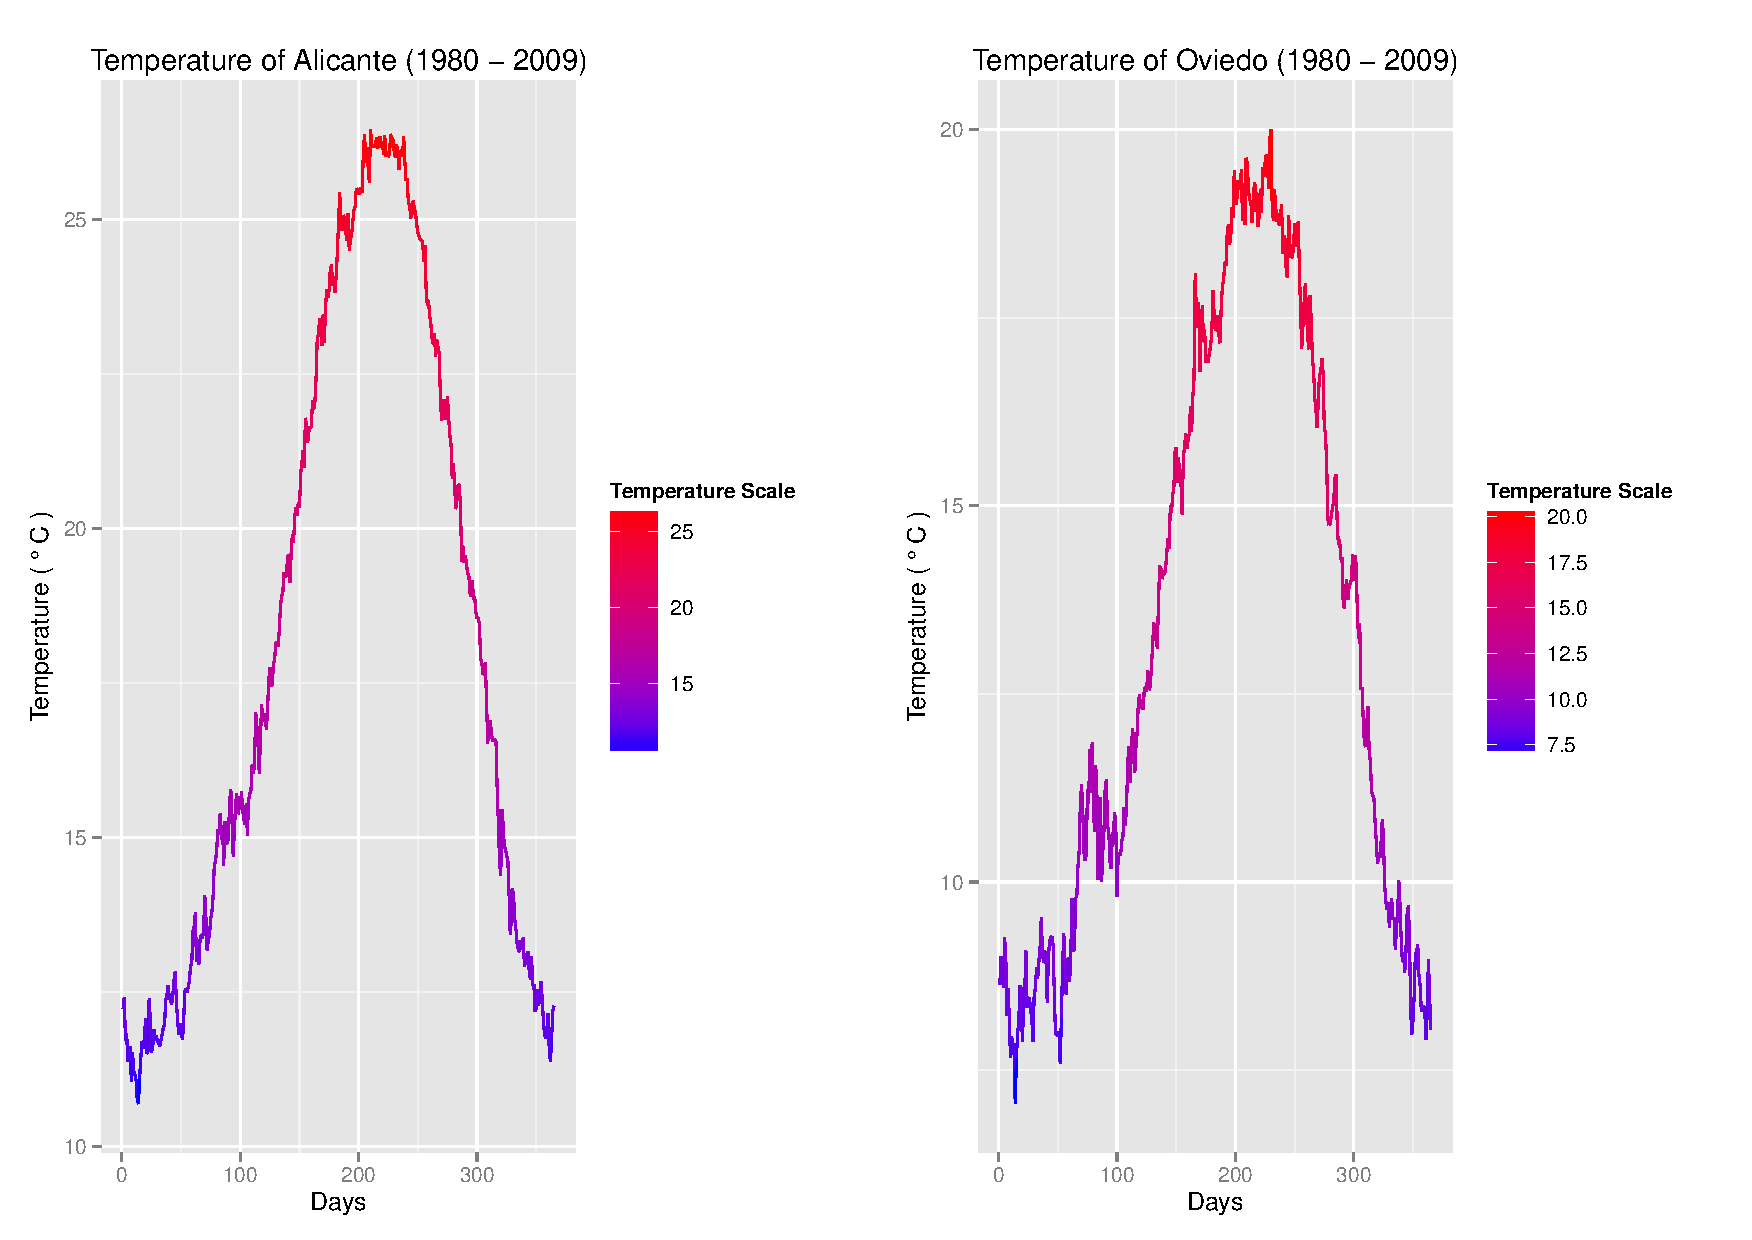
\includegraphics[width=1.1\textwidth]{Figures/temp_plot.pdf}
%    \rule{35em}{0.5pt}
  \caption[Temperature data from \texttt{Alicante} \& \texttt{Oviedo}]{Temperature data from \texttt{Alicante} \& \texttt{Oviedo} stations in Spain (1980 - 2009)}
  \label{fig:FDA1}
\end{figure} 
 In regression problems, it is very likely that the true function $X(t) = \mathbb{E}(Y|t \in \mathcal{T})$ is a nonlinear function of $t$. Representing $X(t)$ by a linear model is usually appropriate, and sometimes a necessary approximation. It is convenient because a linear model is easy to interpret and is the first-order Taylor approximation to $X(t)$ \citep*{hastie_09_elements-of.statistical-learning}. In practice, it is impossible to observe the functional values in continuous time. Smoothing methods using basis expansions are used to trim the erratic pattern of the stochastic process. They provide a good approximation to Functional Data given that the basis functions have the same essential characteristics as the process generating the data, hence minimizing the noise in raw data for calculations and analysis.\\ 
There are several types of basis expansions that can be applied to Functional Data.
\clearpage
%---------------------------------------------------------------------------------------
%	SECTION 2
%---------------------------------------------------------------------------------------

\section{Smoothing Techniques using Basis Expansion}\label{basis_expansion}

As stated in the previous section, the first step in FDA is to reconstruct the functional form of the sample curves from their discrete observations. The sample curves are assumed to be observations of a stochastic process $X = \left\lbrace X(t):t \in \mathcal{T} \right\rbrace$ whose sample functions belong to the Hilbert space $L^{2}(T)$ of square integrable functions with the inner product $\langle X_{1},X_{2} \rangle_{L_{2}} = \int\limits_{\mathcal{T}}X_{1}(t)X_{2}(t)dt,\text{ } \forall X_{1},X_{2} \in L^{2}(\mathcal{T})$. From the previous section, we have seen that any stochastic process can be approximated by taking a weighted sum or \textit{linear combination} of a sufficiently large number \textit{K}. Equation \eqref{fda_21} is written as follows:

\begin{equation}\label{fda_23}
   X_{i}(t) \approx \mathbf{c}^{T}_{i}\boldsymbol\phi(t),\text{ }\forall t \in \mathcal{T},\text{ } i = 1,\dots,N
\end{equation}

where $\mathbf{c}_{i} = \begin{bmatrix}
c_{i1}\\
c_{i2}\\
\vdots\\
c_{iK}
\end{bmatrix}$ and $\bm{\phi}(t) = \begin{bmatrix}
\phi_{1}(t)\\
\phi_{2}(t)\\
\vdots\\
\phi_{K}(t)
\end{bmatrix}$. Equation \eqref{fda_23} can be written in matrix notation as:
\begin{equation}\label{fda_24}
   X_i(\bm{t}_i) \approx \bm{\Phi}(\bm{t}_i) \mathbf{c}_i,\text{ }\forall t \in \mathcal{T}.
\end{equation}

where $\mathbf{\Phi}(\bm{t}_i)=\begin{pmatrix}
\phi_{1}(t_{i1}) & \dots & \phi_{K}(t_{i1})\\
\vdots & \ddots & \vdots\\
\phi_{1}(t_{i1}) & \dots & \phi_{K}(t_{iJ})
\end{pmatrix}$ is a $J \times K$ matrix of basis functions evaluated at each time point $t_j$.\\
Basis functions expansion represent the potentially infinite-dimensional universe of functions within the finite-dimensional framework of vectors like $\mathbf{c}$ \citep{olberd:ramsay}. A great deal depends on how the vector of basis functions $\bm{\phi}(t)$ is chosen.
\clearpage

\subsection{Fourier Basis}
The most appropriate basis for periodic functions defined on an interval $\mathcal{T}$ is the \textit{Fourier Basis} where the $\phi_{k}$'s take the following form:
\begin{equation}\label{fouriereq}
   \phi_{o}(t) = 1/\sqrt{|\mathcal{T}|},\; \phi_{2r-1}(t) = \dfrac{sin(r\omega t)}{\sqrt{|\mathcal{T}|/2}} \; \text{and} \; \phi_{2r}(t) = \dfrac{cos(r\omega t)}{\sqrt{|\mathcal{T}|/2}}
\end{equation}
for $r=1,\dots,\frac{K-1}{2}$, where $K$ is the number of basis functions; notice that the $K$ must be an odd number to compute \textit{Fourier Basis}. The frequency $\omega$ determines the period and the length of the interval $|\mathcal{T}|=2\pi/\omega$. The function vector $\bm{\phi}(t)$ has the form $\bm{\phi}(t) = \left[\phi_{0}(t),\phi_{1}(t),\phi_{2}(t),\dots,\phi_{2r}(t)\right]^T$ evaluated at discrete time points $t_{j}, \text{ }j=1,\dots,J$.\\
The \textit{Fourier Basis} defined above is said to be orthogonal if the values of $t_{j}$ are equally spaced on $J$ and the period is equal to the length of $\mathcal{T}$. Because of the orthogonal property, the cross-product $\mathbf{\Phi^{T}\Phi}$ is diagonal and can be made equal to the identity by dividing the basis function by suitable constants $n^{1/2}$ for $j=0$ and $(n/2)^{1/2}$ for all $j$. This basis is well known partially due to the Fast Fourier Transform (FFT) Algorithm which makes it possible to compute all the coefficients speedily and efficiently. The figures below are plots of the \textit{Fourier Basis} with different $K$-values over the interval $\left[0,365\right]$.

\begin{figure}[h]
  \centering
    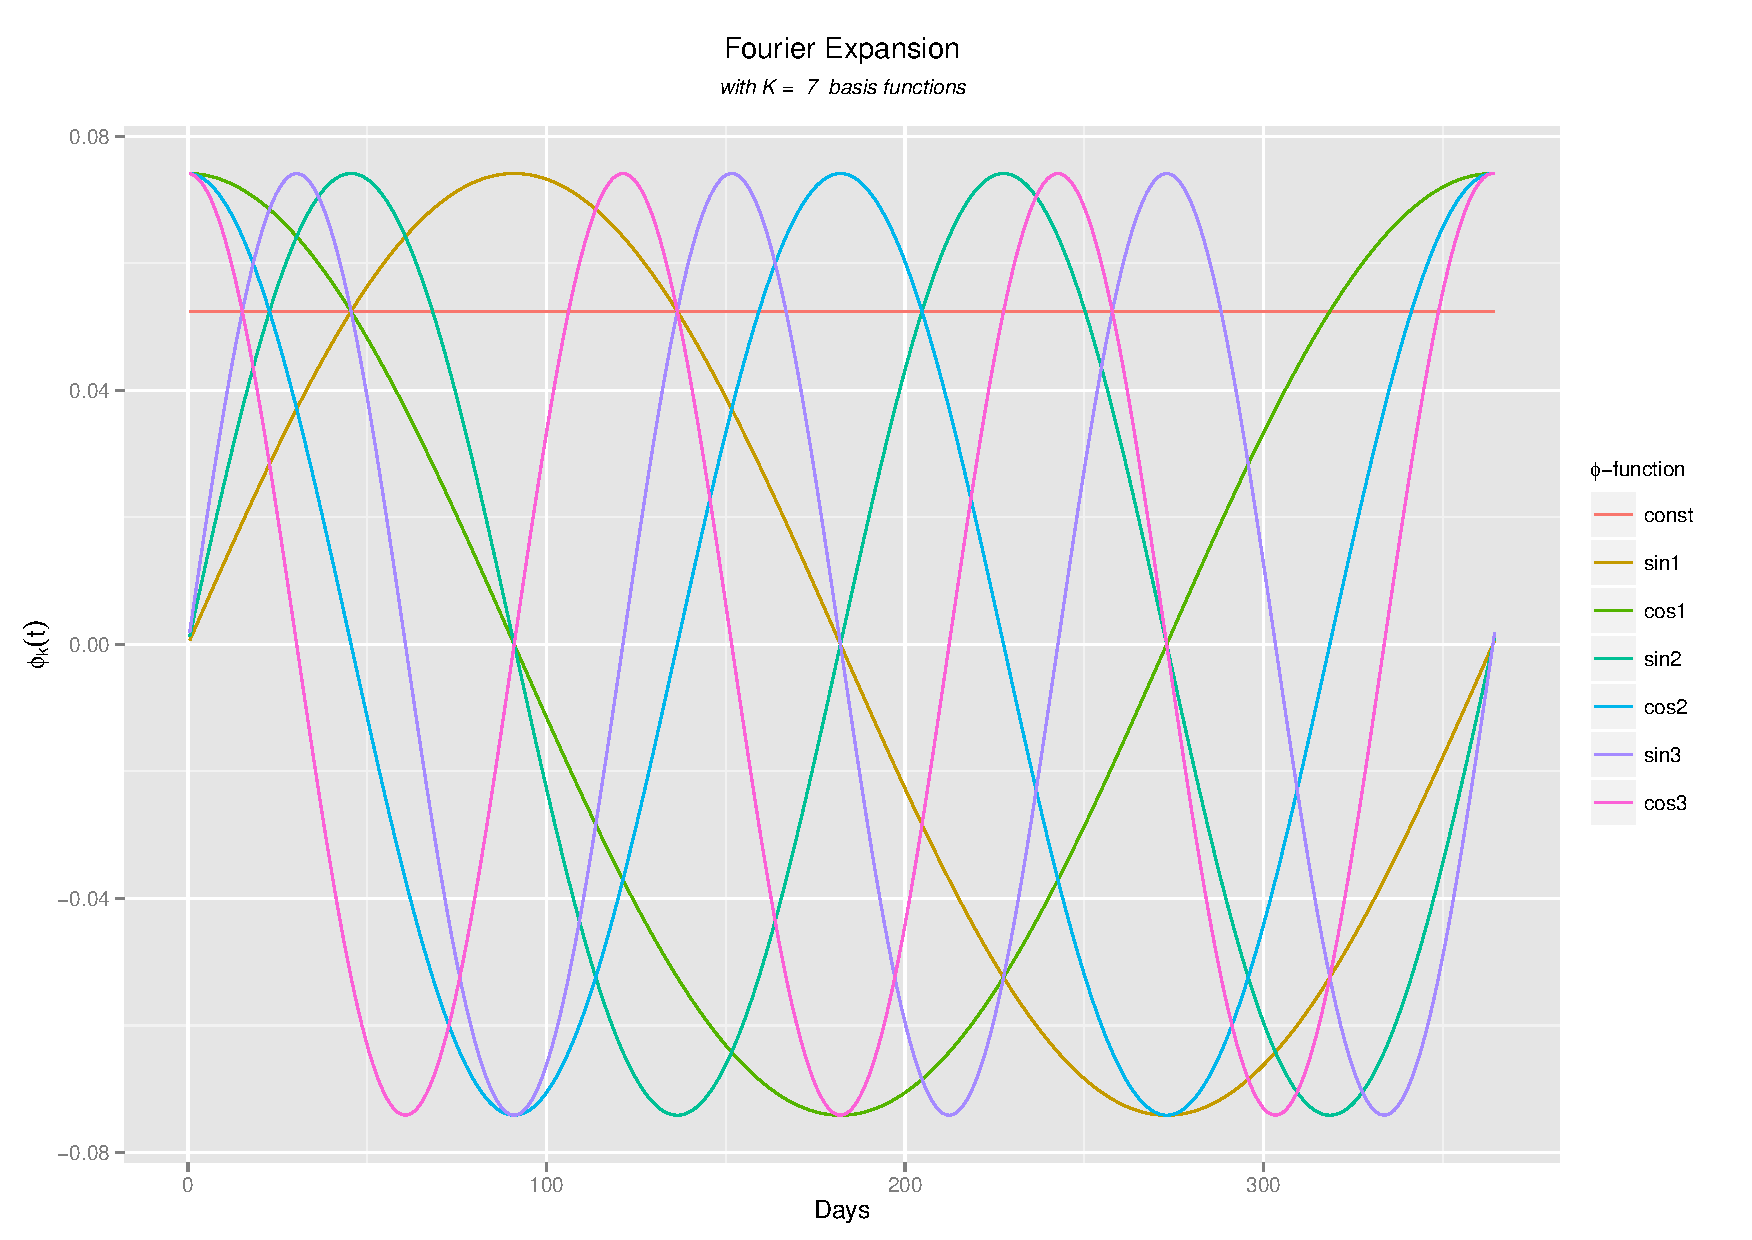
\includegraphics[height=9cm, width=1\textwidth]{Figures/FourierK7.pdf}
%    \rule{35em}{0.5pt}
  \caption[\textit{Fourier Basis} with \textit{K}=7.]{\textit{Fourier Basis} defined over the interval $\left[0,365\right]$.}
  \label{fig:FDA2}
\end{figure}

\begin{figure}[h]
  \centering
    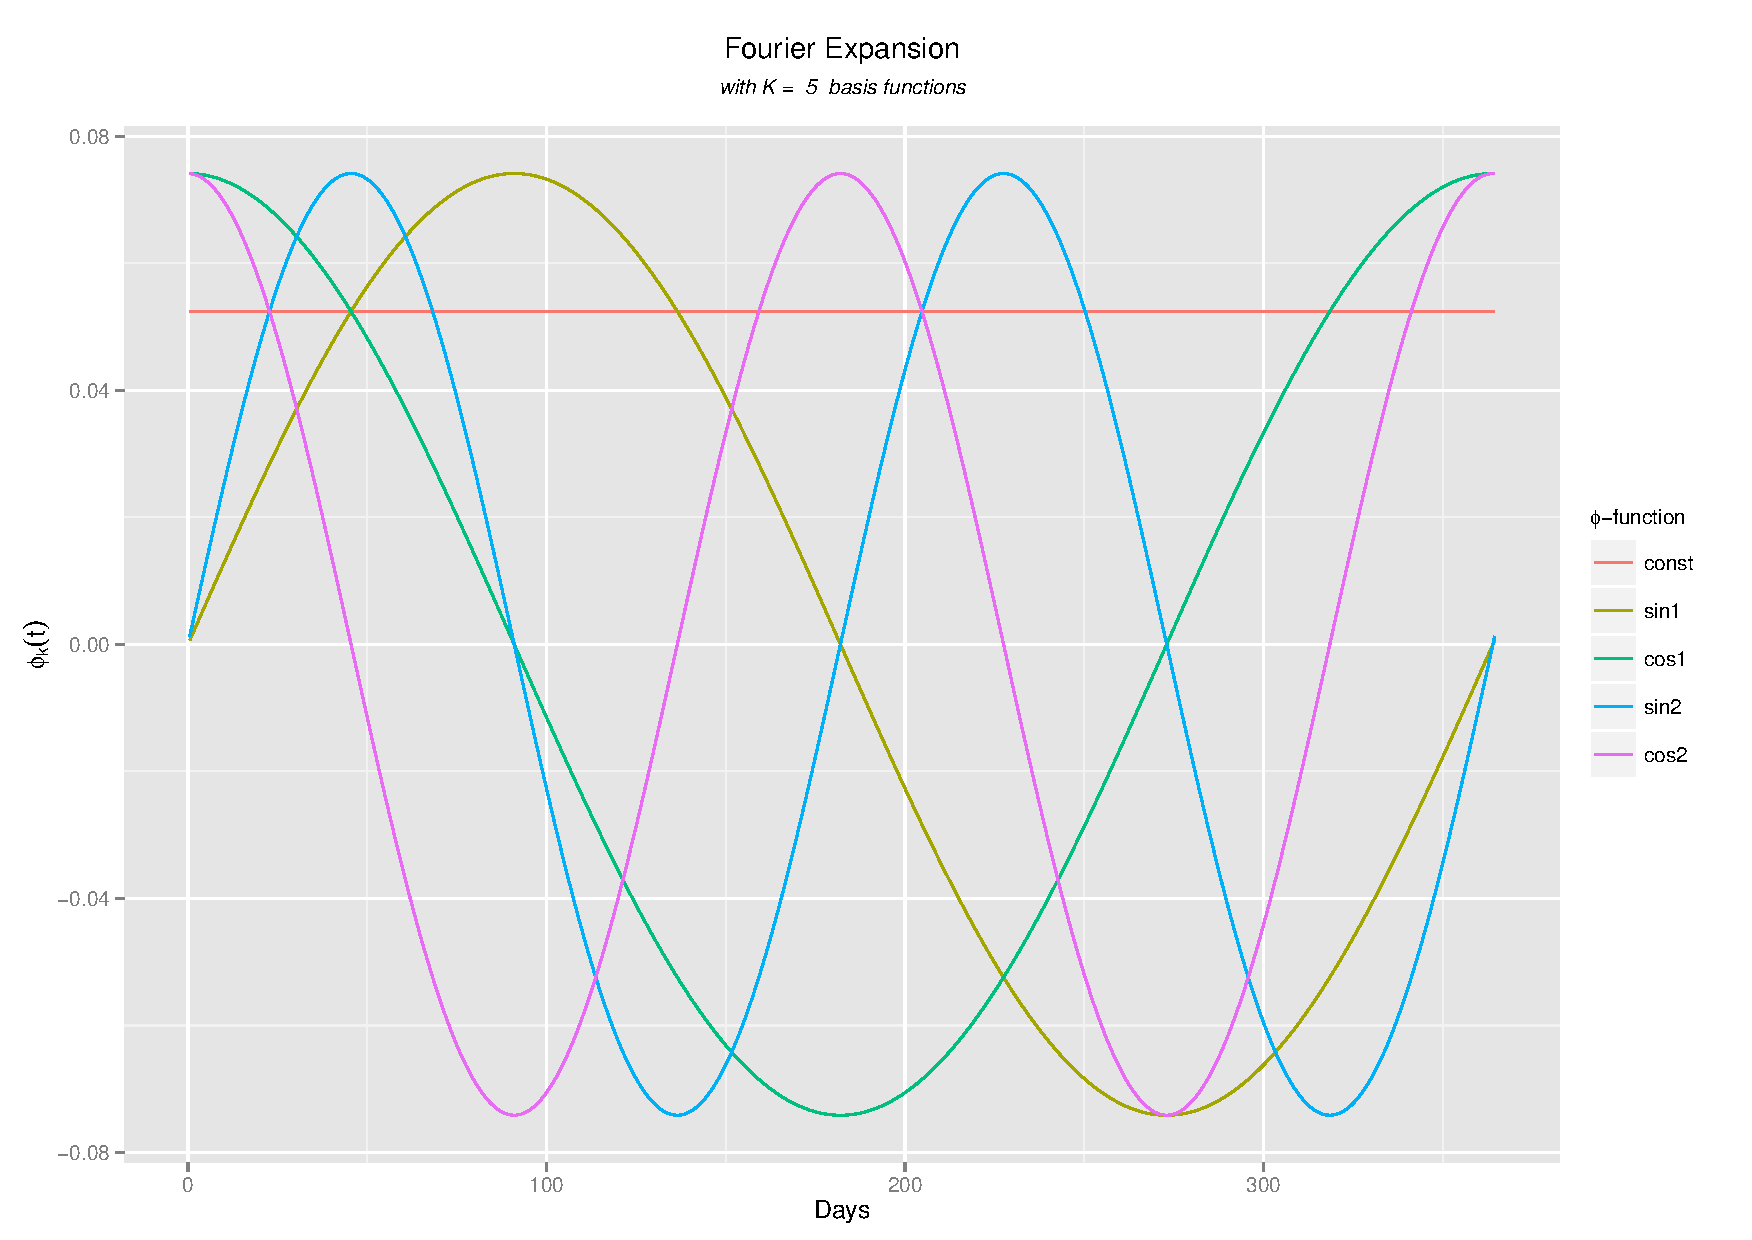
\includegraphics[height=9cm, width=1\textwidth]{Figures/FourierK5.pdf}
%    \rule{35em}{0.5pt}
  \caption[\textit{Fourier Basis} with \textit{K}=5.]{\textit{Fourier Basis} defined over the interval $\left[0,365\right]$.}
  \label{fig:FDA11}
\end{figure}

Figure~\ref{fig:FDA112} illustrates the smoothing of the \textit{Temperature} data in the \texttt{Oviedo} using a \textit{Fourier Basis} with $K = 121$, $K = 51$ and $K = 5$.

\begin{figure}[h]
  \centering
    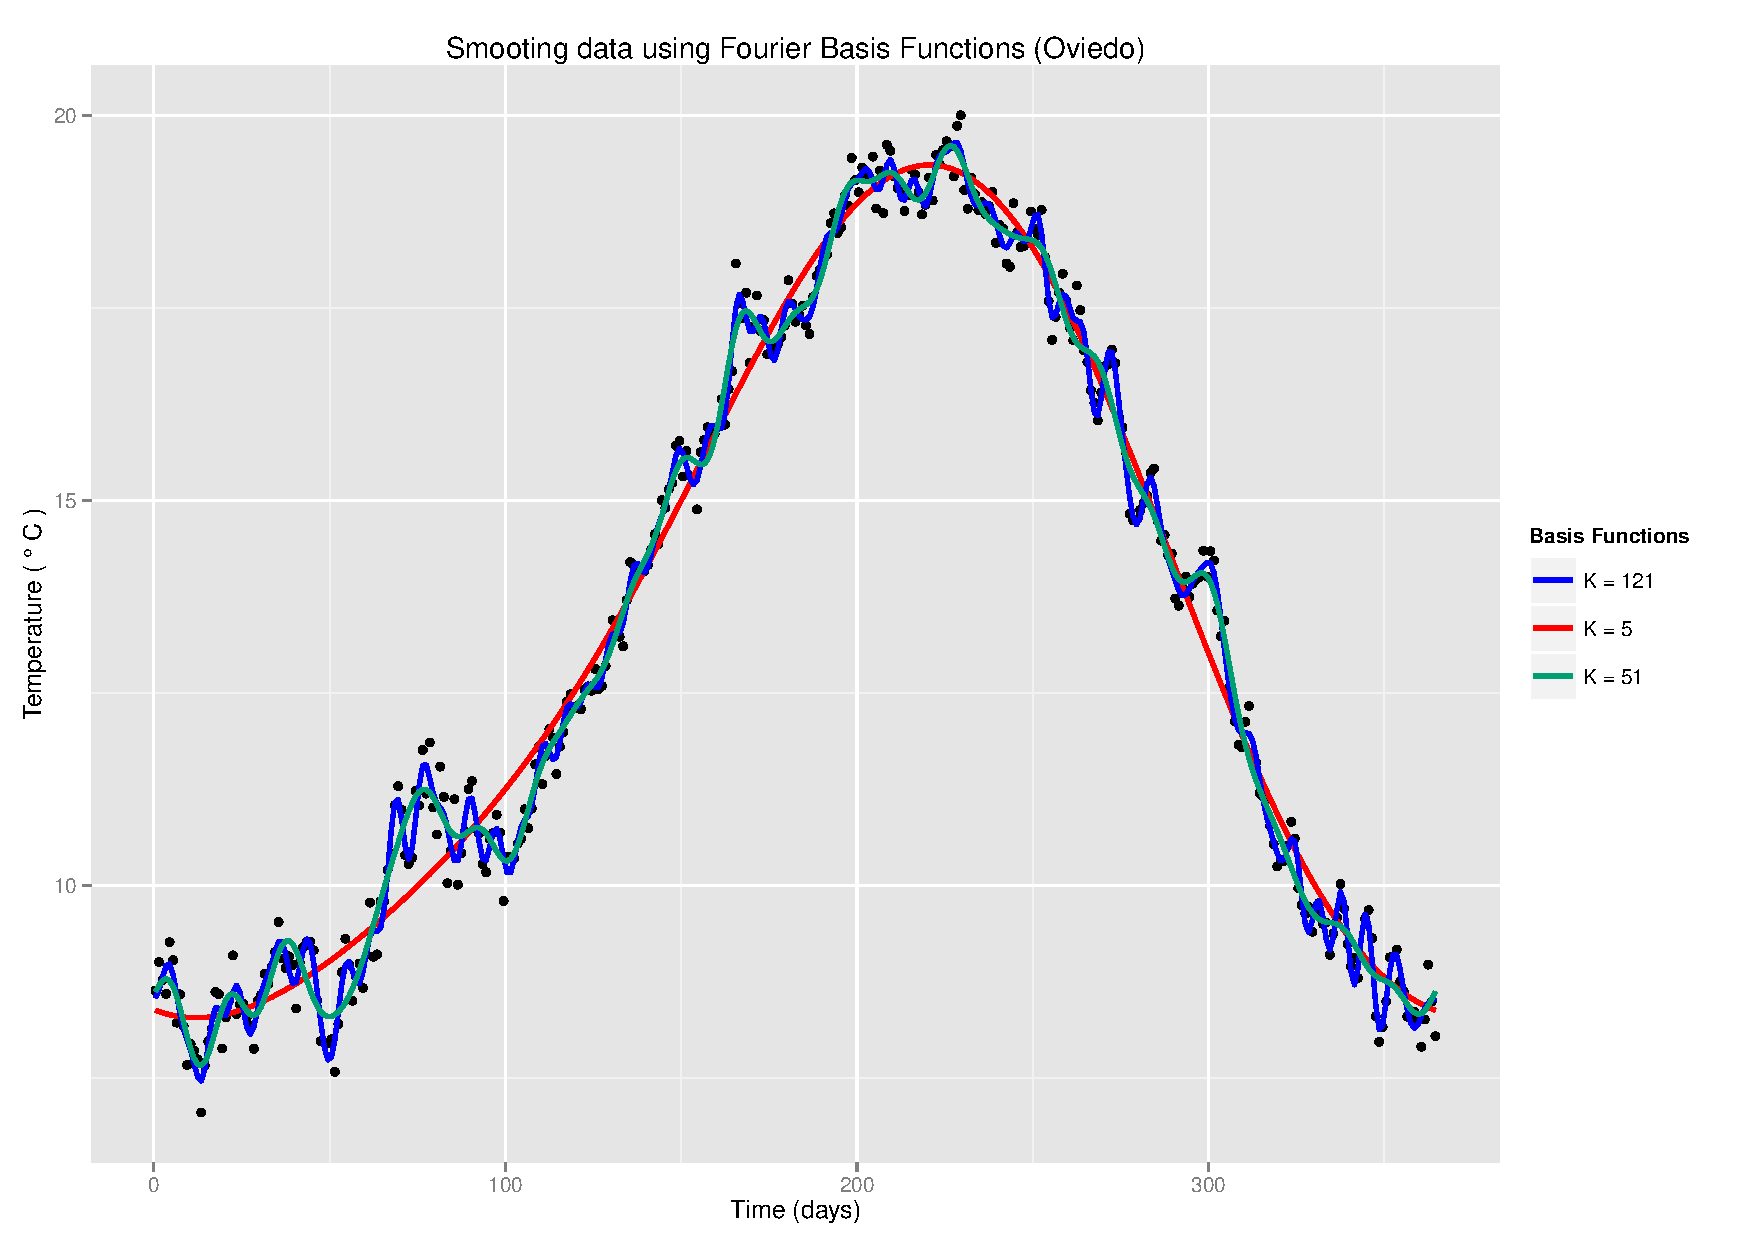
\includegraphics[height=9cm, width=1\textwidth]{Figures/Fourier_Oviedo.pdf}
%    \rule{35em}{0.5pt}
  \caption[\textit{Fourier Basis} applied on Oviedo Temperature data]{\textit{Fourier Basis} applied on Oviedo Temperature data $\left[0,365\right]$.}
  \label{fig:FDA112}
\end{figure}  
\\
\subsection{B-Splines Basis}
Originally derived by \cite{DeBoor2001}, the set of basis splines is a well-known \textit{Functional Basis} for non-periodic data. They are linear combinations of spline functions of specified order over a specified number of breakpoints. A spline is a piecewise polynomial function of order \textit{m} over each interval, which is smoothly connected at breakpoints. More precisely, the interval $\mathcal{T}$ on which the basis is defined is divided into $L$ subintervals separated by values $\tau_{l}, l=0,\dots,L$ called breakpoints or knots. Let $B_{k,m}(t)$ denote the $k$-th \textit{B-Splines Basis} function of order $m$ defined for any value of $t$, for the non-decreasing sequence of knots $\{ \tau_{l} \}_{l=0}^{L}$.
\vskip
\setlength{\parindent} In this case, $\phi_{k}(t)$ is defined as follows:
\begin{equation}
\phi_{k}(t)= B_{k,m}(t),\text{ }\forall t \in \mathcal{T},\text{ } k=1,\dots,m+L-2
\end{equation}

Let $\xi_0 < \xi_1$ and $\xi_K < \xi_{K+1}$ be two boundary knots defining the domain over which the spline is evaluated. The augmented knot sequence $\tau$ is defined as:

\begin{itemize}
\item $\tau_1 \leq \tau_2 \leq \dots \leq \tau_M \leq \xi_0$;
\item $\tau_{j+M} = \xi_j, \text{ }j = 1,\dots,K$;
\item $\xi_{K+1} \leq \tau_{K+M+1} \leq \tau_{K+M+2} \leq \dots \leq \tau_{K+2M}$.
\end{itemize}
Any additional knots beyond the boundary are abitrary, and the usual scenario is to make them all the same an equal to $\xi_0$ and $\xi_{K+1}$.
The set of basis functions $B_{k,m}(t)$ of order $m$ for the knot-sequence $\tau$ (where $m < M$) is derived using a recursion formula as follows:

\begin{eqnarray}
B_{k,1}(t) = \left\{ 
\begin{array}{cc}
1, & \quad \textrm{ } t\in [\tau_{l},\tau_{l+1}]\\
0, & \quad \textrm{otherwise}
\end{array}\right.
\end{eqnarray}
for $k = 1,\dots,K+2M-1$. These functions are called Haar basis functions. 
\begin{equation}
B_{k,m}(t)=\frac{t-\tau_{l}}{\tau_{k+m-1}-\tau_{k}}B_{k,m-1}(t)+\frac{\tau_{k+m}-t}{\tau_{k+m}-\tau_{k+1}}B_{k+1,m-1}(t),\text{ }\forall t \in \mathcal{T},\text{ } m \geq 2 .
\end{equation} for $k = 1,\dots,K+2M-m$.
In this case, the function vector $\bm{\phi}(t)$ defined in equation~\eqref{fda_23} has $K+2M-m$ basis functions evaluated at discrete time points $t_{j}, \text{ where }j=1,\dots,J$. \\In other words, the number of basis functions is defined by its order and its number of knots. The main advantages of the \textit{B-Splines Basis} are its flexibility as well as its fast computation.

\begin{figure}[h]
  \centering
    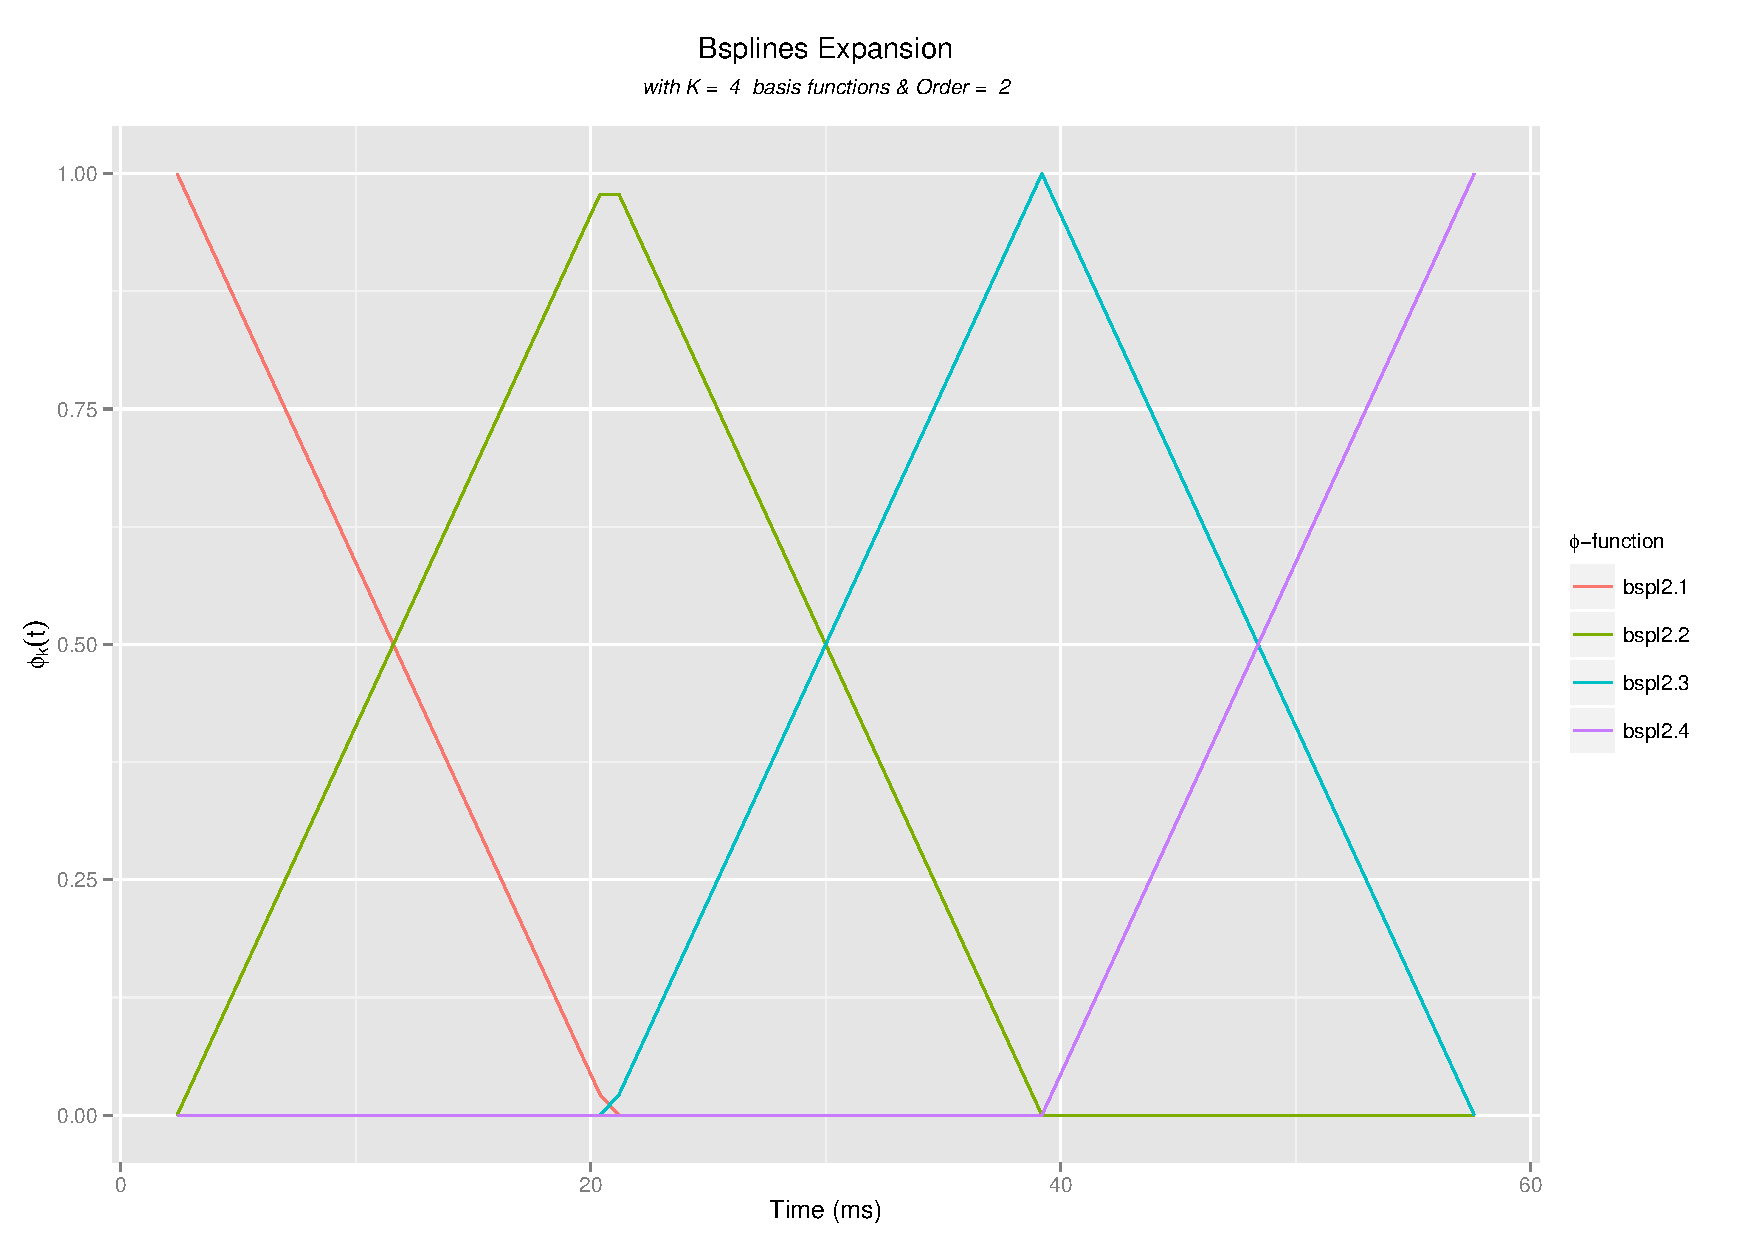
\includegraphics[height=9cm, width=1\textwidth]{Figures/BsplineK4o2.pdf}
%    \rule{35em}{0.5pt}
  \caption[\textit{B-Splines Basis} of order 2 with 4 basis functions]{\textit{B-Splines Basis} of order 2 with 4 basis functions}
  \label{fig:FDA3}
\end{figure}
%\clearpage

\begin{figure}[h]
  \centering
    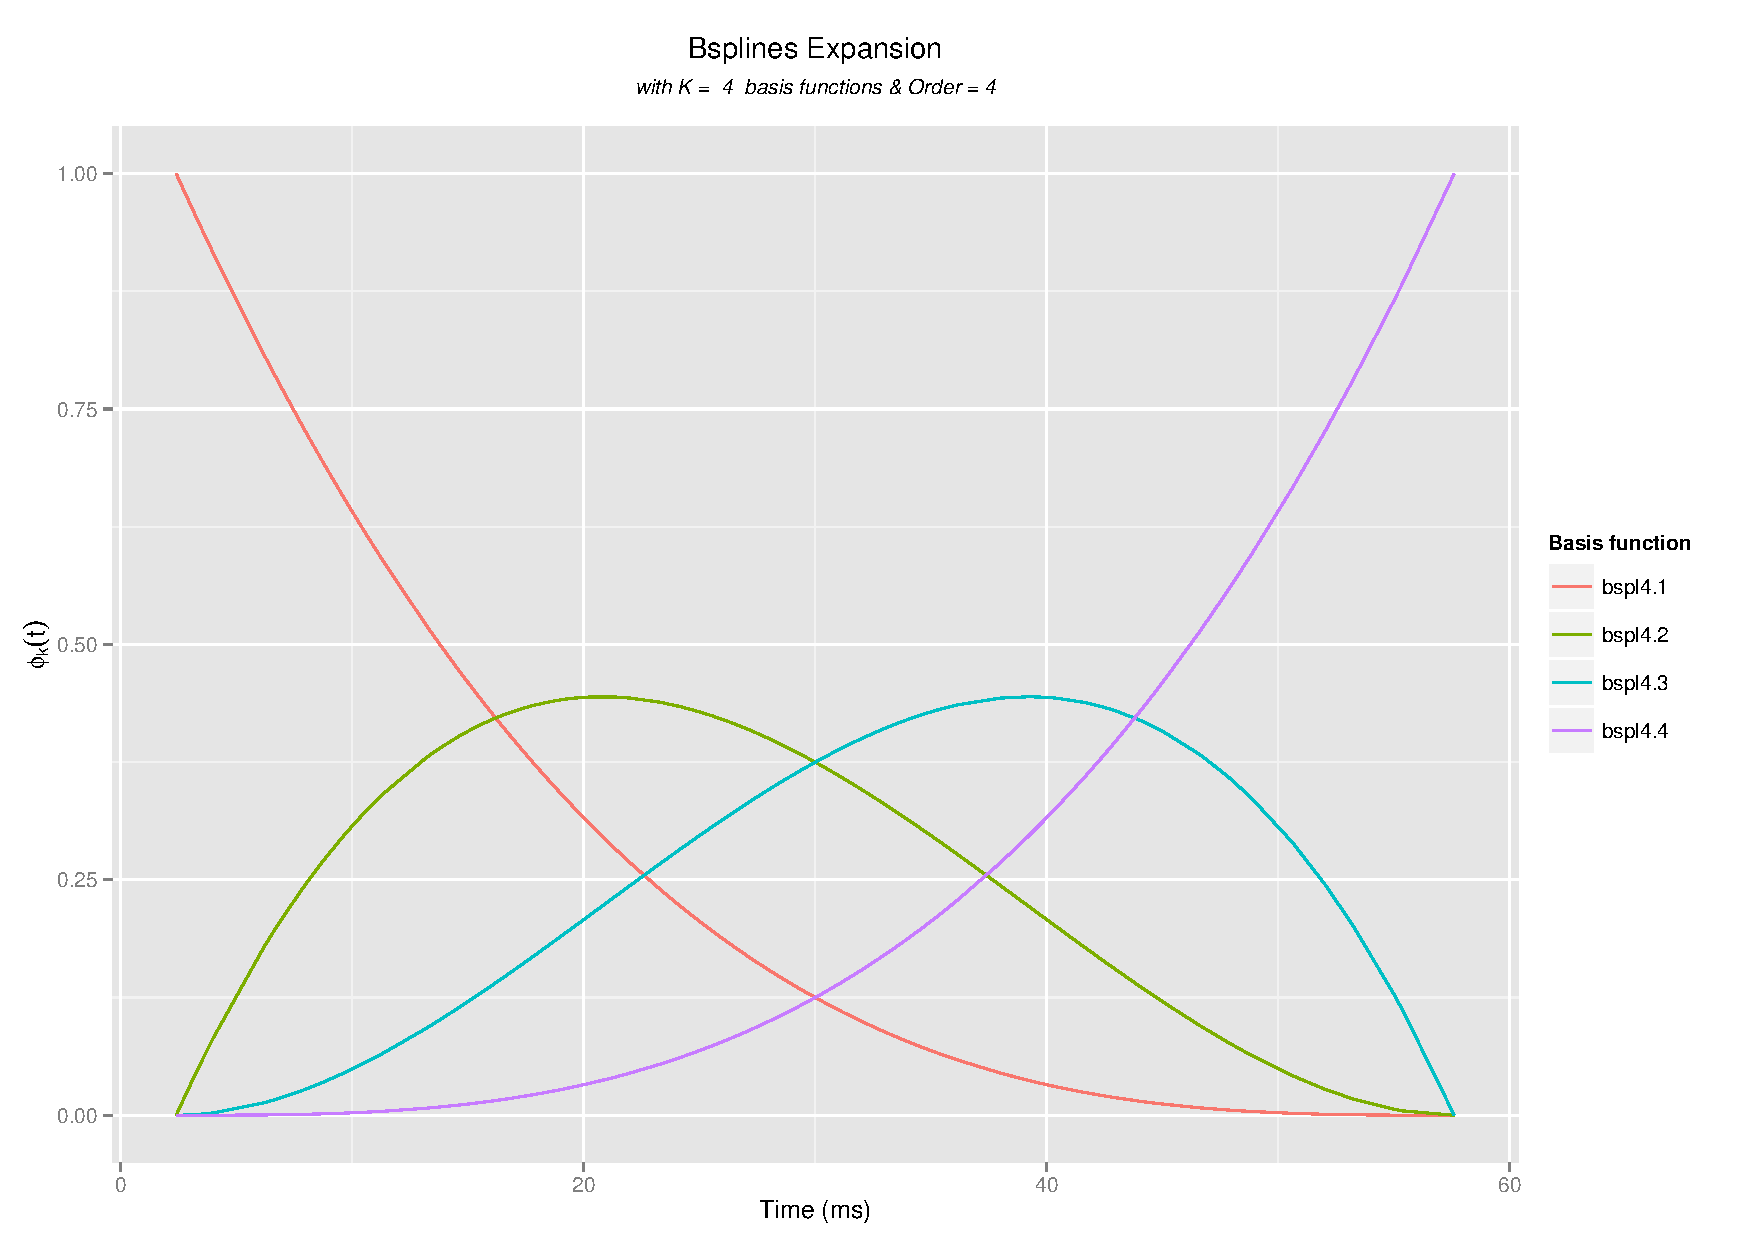
\includegraphics[height=9cm, width=1\textwidth]{Figures/BsplineK4o4.pdf}
%    \rule{35em}{0.5pt}
  \caption[\textit{B-Splines Basis} of order 4 with 4 basis functions]{\textit{B-Splines Basis} of order 4 with 4 basis functions}
  \label{fig:FDA41}
\end{figure}
\clearpage

Smoothed estimates of the observed data are derived when applying this smoothing technique onto a non-periodic dataset, but it depends on the parameter $K$. For illustration, consider the \texttt{Motorcycle Data} which has been widely used by \citet{Silverman1985} and \citet{Hardle94}. For more information on the dataset, refers to the \texttt{R}-package \texttt{adlift} created by \cite{Motordata}. Figure~\ref{fig:FDA42} depicts the \texttt{Motorcycle Data} smoothed with the \textit{B-Splines} function for $K = 20$ and $K = 40$. 

\begin{figure}[h]
  \centering
    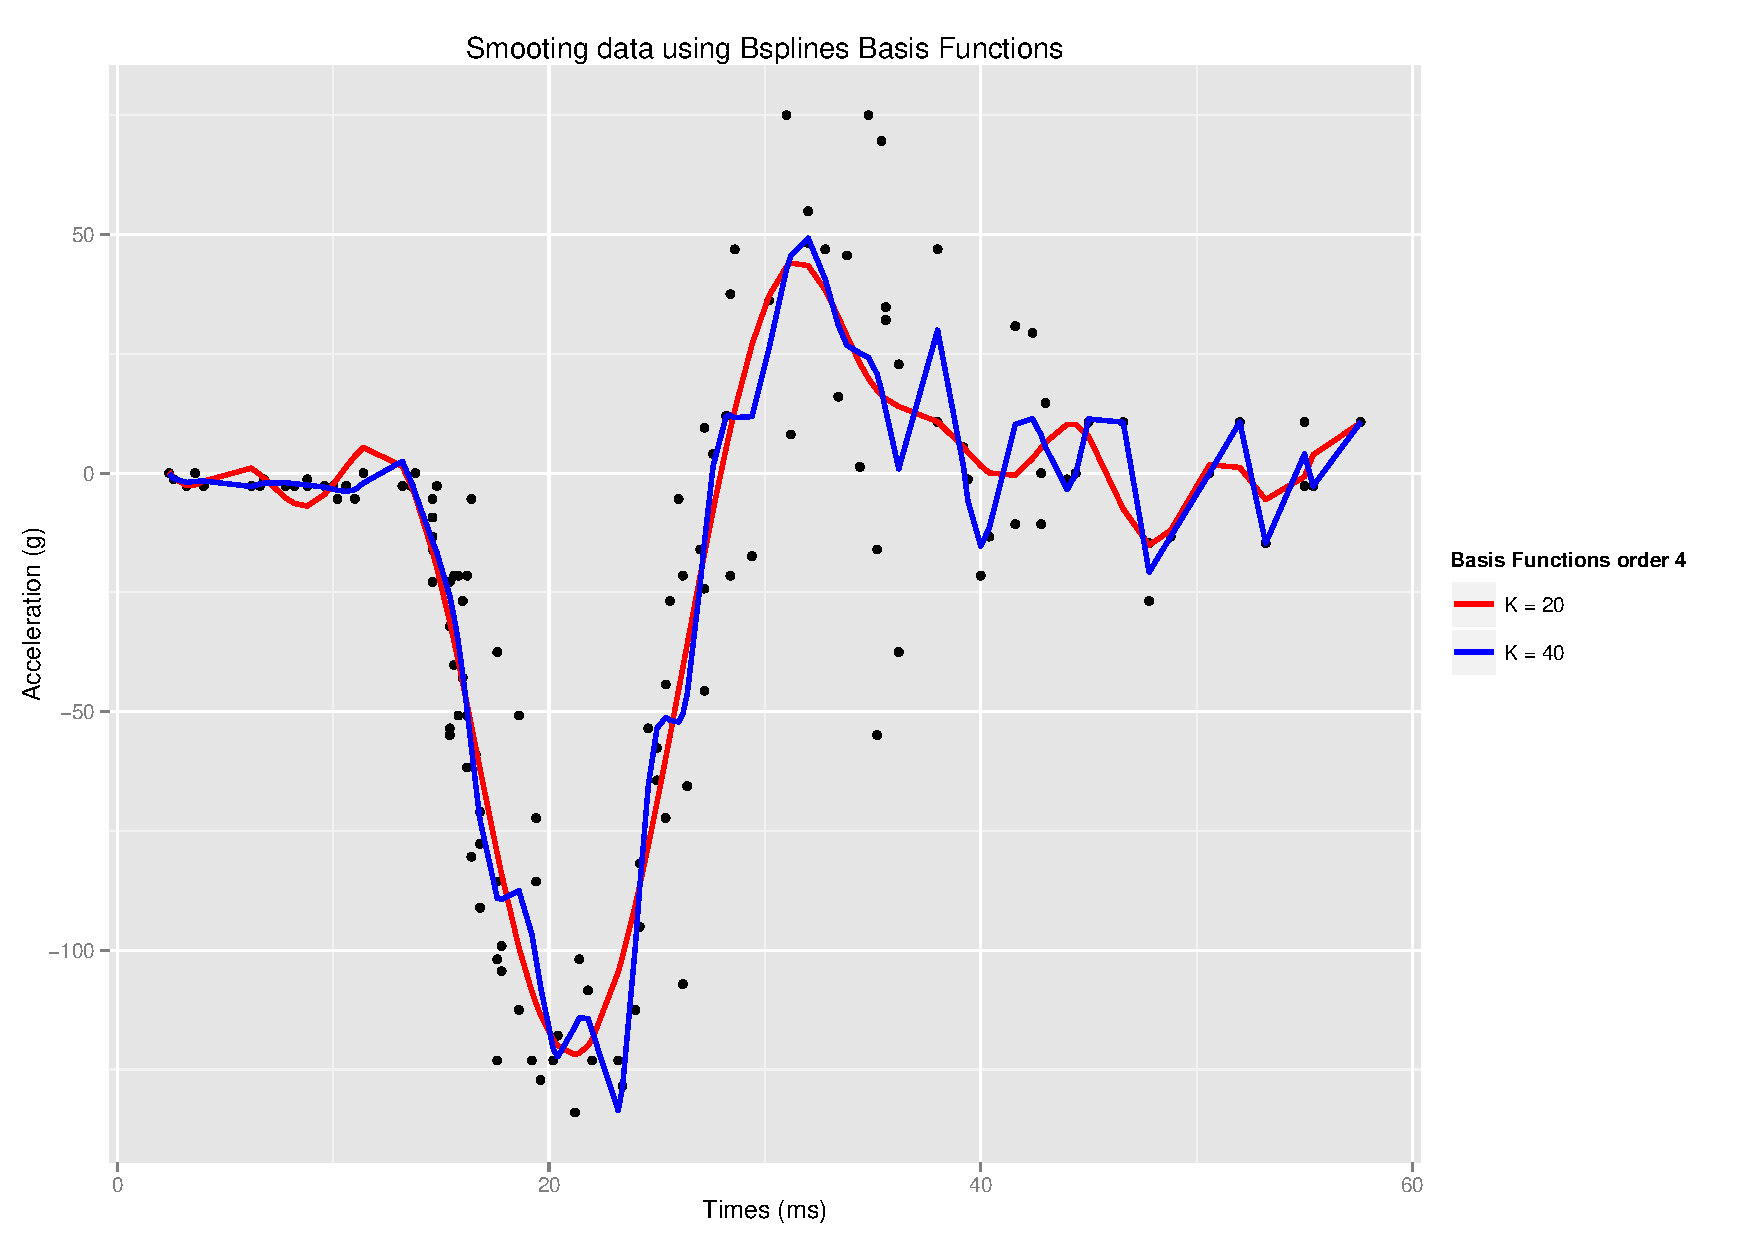
\includegraphics[height=9cm, width=1\textwidth]{Figures/Bsplines_Motorcycle1.pdf}
%    \rule{35em}{0.5pt}
  \caption[\textit{B-Splines Basis} Basis applied on the \texttt{Motorcycle Data}]{\textit{B-Splines Basis} Basis applied on the \texttt{Motorcycle Data}}
  \label{fig:FDA42}
\end{figure}

\subsection{Gaussian Radial Basis Functions}

Radial basis functions is a class of single hidden layer feedforward networks which can be expressed as a linear combination of radially symmetric nonlinear basis functions \citep{Ando2008}. Each basis function forms a localized receptive field in the input space. The most commonly used function is the \textit{Gaussian Basis} functions which is given by:

\begin{equation}
\phi_k(t;\mu_k ,\sigma^2_k) = \exp \left(-\dfrac{||t-\mu_k||^2}{2\sigma^2_k}\right),\textbf{ } k=1,\dots,K
\end{equation}
where $\mu_k $ is a parameter determining the center of the basis function, $\sigma^2_k $ is a parameter that determines the width and $||.||$ is the Euclidian norm. \textit{Gaussian Basis} functions have a number of useful analytical and practical properties (see \cite{Bishop1995}). The basis functions overlap with each other to capture the information about \textbf{t}. More importantly, the width parameter play an essential role to capture the structure in the data over the region of input data. The parameters featuring in each basis function are often determined heuristically based on the structure of the observed data.\\
\cite{Moody1989} used the \texttt{K-means} clustering algorithm to determine both the center and the width parameter of the basis function. This algorithm splits the observational space $\mathcal{T}$ into $K$ clusters $\{C_1,C_2,\dots,C_K\}$ that correspond to the number of basis functions. They are determined by:
\begin{equation}
\hat{\mu}_k = \frac{1}{N_k}\sum_{t_j \in C_k} t_j, \text{  } \hat{\sigma}^2_k = \dfrac{1}{N_k}\sum_{t_j \in C_k} ||t_j - \hat{\mu}_k||^2,
\end{equation}

where $N_i $ is the number of observations which belongs to the $k^{th}$ cluster. However, this method does not produce unique parameters for a unique set of observations, due to the stochastic nature of the starting value in the clustering algorithm. Because of that feature, the \textit{K-means} clustering underperforms when capturing all the information from the data. This is noticeable when the set of Functional Data are observed at equidistant points.\\ \cite{Ando2008} proposed to include the hyper-parameter $\nu$ ($> 0$) to control the amount of overlapping as a mean to overcome the lack of overlapping among basis functions. The transformed \textit{Gaussian Basis} are now given by:

\begin{equation}
\phi_k(t;\mu_k ,\sigma^2_k) = \exp \left(-\dfrac{||t-\mu_k||^2}{2\nu \sigma^2_k}\right),\textbf{ } k=1,\dots,K
\end{equation}

In order to stabilize the estimation of the Gaussian basis functions parameters, \cite{kawano2007} proposed basis functions where the centers and the width parameters are determined by preassigned knots similar to \textit{B-Splines} basis functions. Consider the observations $\{x_j;\text{ } j=1,\dots,n\}$ arranged by magnitude, the knots $t_k\text{ }(k = 1,\dots,K+4)$ are set up as follows:
\begin{equation}
t_1 < t_2 < t_3 < t_4 = x_1 < t_5 < \dots < t_K < t_{K+1} = x_K < t_{K+2} < t_{K+3} < t_{K+4}
\end{equation}
where the knots are equally spaced. By setting the knots in this way the \textit{n} observations are divided into $(K-3)$ intervals:

\begin{equation}
[t_4,t_5],[t_5,t_6],\dots,[t_K,t_{K+1}].
\end{equation}
The \textit{Gaussian Basis} functions are now defined with a center $t_k$ and a width $h = (t_k - t_{k-2})/3$ for $k = 3,\dots,K+2$ as follows:
\begin{align} 
\begin{split}
\phi_k(x;t_k ,h^2) &= \exp \left(-\dfrac{||x-t_k||^2}{2 h^2}\right)\\
h 	&= \dfrac{t_k - t_{k-2}}{3}, \text{  } k = 3,\dots,K+2\\
\end{split}					
\end{align}

Figure~\ref{fig:FDA45} shows two different \textit{Gaussian Basis} functions (with 8 functions) plotted on the same set of observations. Note that the areas under the curves for \textit{K-means} clustering are different, whereas the areas for \textit{Gaussian Basis} using \textit{B-Splines} approach are consistent.

\begin{figure}[h]
  \centering
    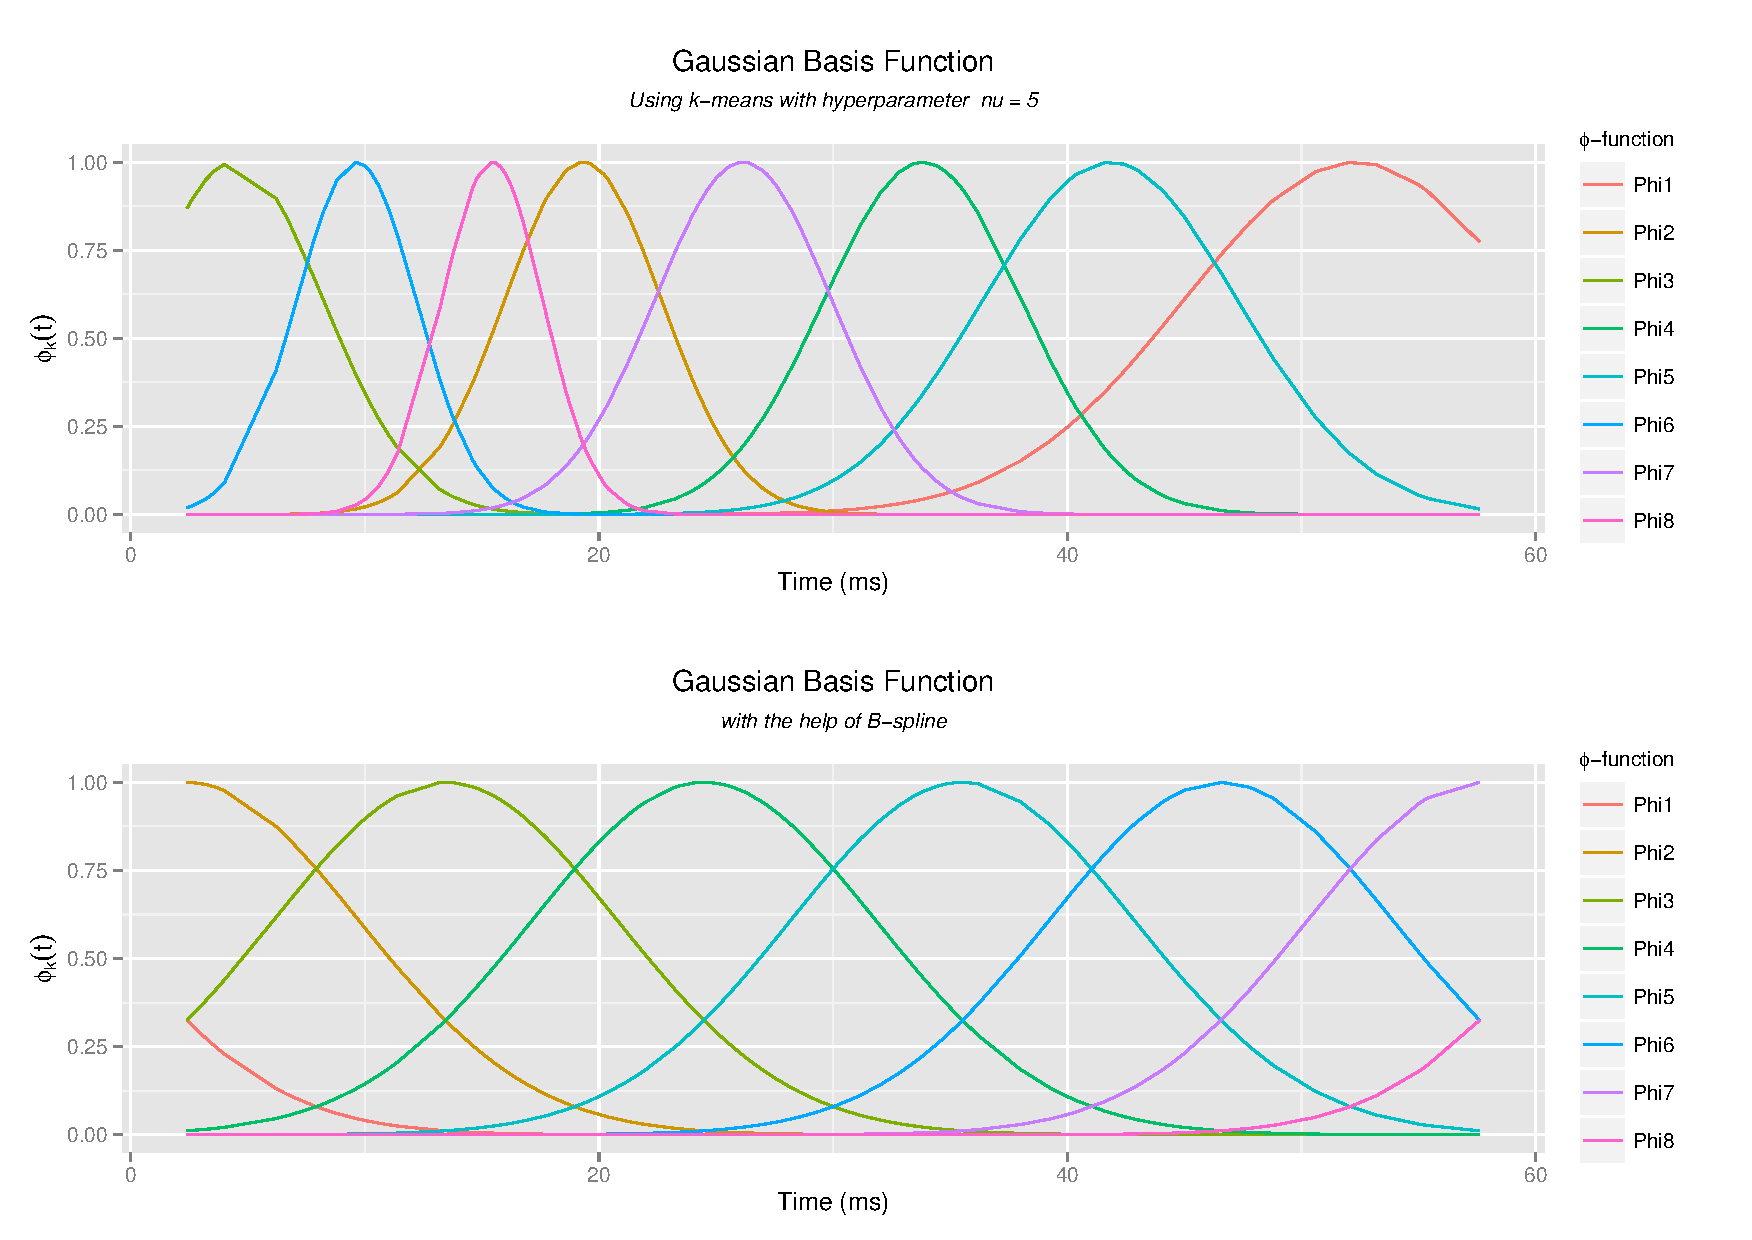
\includegraphics[height=14cm, width=1\textwidth]{Figures/gaussian_motor1.pdf}
%    \rule{35em}{0.5pt}
  \caption[Contrast between \textit{K-means} clustering method and \textit{B-Splines} method]{Contrast between \textit{K-means} clustering method and \textit{B-Splines} method}
  \label{fig:FDA45}
\end{figure}
\clearpage
Figure~\ref{fig:FDA4} shows smooth curves obtained when applying the abovementioned methods on the motorcycle impact data using the following basis functions: (1)\textit{Gaussian Basis} using \textit{B-Splines} (K = 20);  (2) \textit{Gaussian Basis} using \textit{K-means} (K = 20, $\nu = 2$).

\begin{figure}[h]
  \centering
    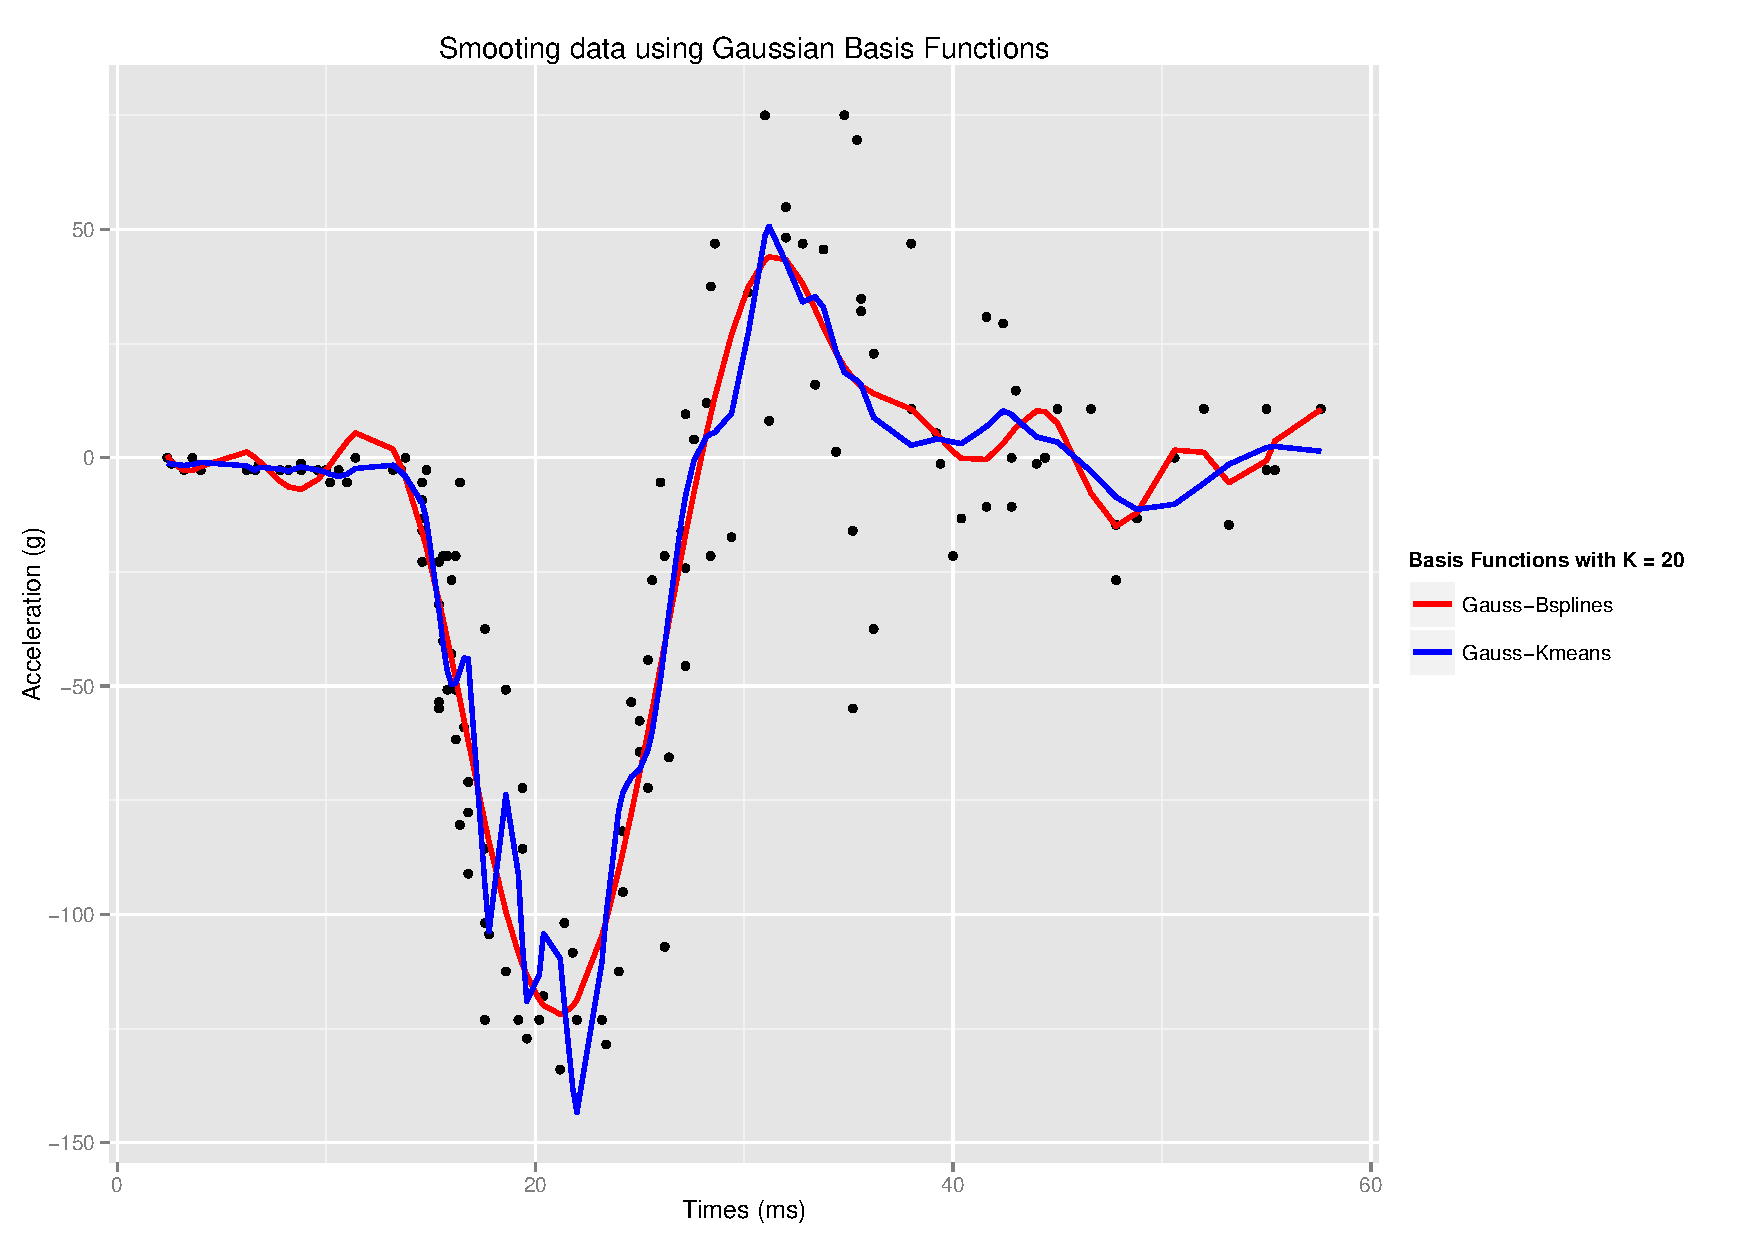
\includegraphics[height=9cm, width=1\textwidth]{Figures/gauss_motorcycle2.pdf}
%    \rule{35em}{0.5pt}
  \caption[Motorcyle impact data fitted with  \textit{Gaussian Basis} functions]{Motorcyle impact data fitted with \textit{Gaussian Basis} functions}
  \label{fig:FDA4}
\end{figure}


\subsection{Other Basis Functions}

Recent developments in the study of Functional Data have led to a number of other potentially important basis systems. For instance, the \textit{Haar Wavelets} which combine the frequency-specific approximating power of the \textit{Fourier Basis} with the time- or spatially-localized features of \textit{Splines}. Another example, \textit{Simple Bases} such as step functions and polynomial bases:
\subsubsection*{Haar Wavelets}
The \textit{Haar Wavelets} transform is useful to model a multiresolution stochastic process. It exploits the idea that a basis is constructed by choosing a suitable scaling function $\phi$ (the \textit{Father Wavelet}) and the function $\psi$ (the \textit{Mother Wavelet}) of the \textit{Haar Wavelets} defined on $[0,1)$. The functions $\phi(t)$ and $\psi(t)$ are given by:
\begin{center}
$\phi(t) =
    \begin{cases}
            1, &         \text{if } 0 \leq t < 1;\\
            0, &         \text{if otherwise};
    \end{cases}$
\end{center}

\begin{center}
$\psi(t) =
    \begin{cases}
            1, &         \text{if } 0 \leq t < 1/2;\\
            -1, &         \text{if } 1/2 \leq t < 1;\\
            0, &         \text{if otherwise}.
    \end{cases}$
\end{center}
The Haar wavelets are then generated in the form of translations and dilations of the above father and mother wavelet functions as
\begin{align}
\phi_{j,k}(t) &= \sqrt{2^j}\phi(2^j t - k), \nonumber \\
\psi_{j,k}(t) &= \sqrt{2^j}\psi(2^j t - k), \nonumber
\end{align}

where $j = 0,1,\dots$ and $k = 0,1,\dots,2^j -1$. The index $j$ refers to dilations and $k$ refers to translations and $\sqrt{2}$ is the normalizing factor. The mother wavelet is constructed to ensure that the basis is orthogonal. The \textit{Wavelet Basis} idea is easily adapted to deal with functions defined on a bounded interval, most simply if periodic boundary conditions are imposed \citep{olberd:ramsay}. The coefficients of $\psi_{jk}$ yield information about $f$ near position $2^{-j}k$ on scale $2^{-j}$. In contrast to \textit{Fourier Basis}, \textit{Wavelet Basis} expansions cope well with discontinuities and rapid changes in behavior, that allows them to accomodate a wide variety of functional forms. See \cite{walker2008} for more details on \textit{Wavelet Basis}.
\subsubsection*{Polynomial bases}
The basis functions could be expressed as $\phi_{k}(t)=\left(t-\omega\right)^{k},\text{ }\forall t \in \mathcal{T}, \text{ }k=0,\dots,n$, where $\omega$ is a shift parameter that is usually chosen to be in the center of the interval of approximation. Like the \textit{Fourier Basis} expansion, \textit{Polynomials Basis} cannot exhibit local features without using a large number of basis functions. They tend to fit well in the center of the data but exhibit rather unattractive behavior around the tails. Although derivatives of \textit{Polynomials Basis} expansion are simple to compute, they are usually a poor basis for extrapolation or forecasting.

\subsubsection*{Kernel Smoothing}
Smoothing problems, in a statistical framework, are appropriate under the consideration that the data set is merely a realization of a random sample from a certain population. For a smoothing method to make sense, the value of the function estimated at a point $\phi(t_{j})$ must be influenced mostly by the observations near that point. An intuitive estimator $\hat{\phi}_{i}(t)$ is the locally weighted average. Generally speaking a kernel smoother defines a set of weights $\{W_{i}^{h}(t)\}^{n}_{i=1}$ for each $t$.
Let $\mathcal{K}$ be a real-valued function assigning weights. The function $\mathcal{K}$, also called the \textit{Kernel} function, is usually a symmetric probability density. Let $h$ be a bandwidth which is a nonnegative number controlling the size of the local neighborhood. \cite{olberd:ramsay} described the \textit{Kernel Basis} as a function that has most of its mass concentrated close to 0, and either decay rapidly or disappear entirely for $|u| \geq 1$. The most popular \textit{kernel} functions are:
\begin{itemize}
\item \textbf{Gaussian:} $\mathcal{K}(u)=\dfrac{1}{\sqrt{2\pi}}\text{exp}\left[-u^{2}/2\right]$
\item \textbf{Epanechnikov:} $\mathcal{K}(u)= \dfrac{3}{4} \mathbbm{1}_{\left[-1,1\right]}(1-u^{2})$
\item \textbf{Triweigth:} $\mathcal{K}(u)= \dfrac{35}{32} \mathbbm{1}_{\left[-1,1\right]}(1-u^{2})^{3}$
\item \textbf{Uniform:} $\mathcal{K}(u)= \dfrac{1}{2} \mathbbm{1}_{\left[-1,1\right]}(u)$
\item \textbf{Cosine:} $\mathcal{K}(u)= \dfrac{\pi}{4} \mathbbm{1}_{\left[-1,1\right]}\cos(\pi \times u/2)$
\item \textbf{Quartic:} $\mathcal{K}(u)=\dfrac{15}{16} \mathbbm{1}_{\left[-1,1\right]}(1-u^{2})^{2}$ 
\end{itemize}
The estimate at a given point is a linear combination of local observations,
\begin{equation*}
\hat{\phi}_{i}(t) = \sum\limits_{j=1}^{p}\hat{W}_{i}^{h}(t_{j})Y_{j}
\end{equation*}
for some suitably defined weight functions $W^{h}(t_{j})$. \citet{Nada1964} and \citet{Wats1964} developed one of the most popular kernel estimator the \textit{Nadaraya-Watson} estimator given by:
\begin{equation}
\hat{W}^{h}(t_{j})=\frac{\sum\limits_{j=1}^{p}\mathcal{K}^{h}(t_{j}-t)Y_{j}}{\sum\limits_{j=1}^{p}\mathcal{K}^{h}(t_{j}-t)}
\end{equation}
where $\mathcal{K}^{h}(.)=\mathcal{K}(./h)/h$. \cite{Gasser1979,GassMull1984} constructed the weights as follows:
\begin{equation}
\hat{W}^{h}(t_{j})=\sum\limits_{j=1}^{p}\int\limits_{\bar{t}_{j}}^{\bar{t}_{j-1}}\mathcal{K}^{h}(u-x)du \times Y_{j}
\end{equation}
with $\bar{t}_{j}=(t_{j+1}+t_{j})/2$, $1 \leq j \leq n$, $\bar{t}_{0} = t_{1}$ and $\bar{t}_{p} = t_{p}$. This estimator was originally proposed for \textit{equispaced designs}, but can also be used for \textit{non-equispaced designs}. Figure~\ref{fig:FDA5} depicts a visualization of \textit{Kernel} smoothing regression.
\begin{figure}[h]
  \centering
    \includegraphics[height=8cm, width=1\textwidth]{Pictures/Untitled.png}
%    \rule{35em}{0.5pt}
  \caption[\textit{Kernel Smoothing} regression at Boundaries]{An illustration of \textit{Kernel Smoothing} regression technique (Image taken from \citealp{hastie_09_elements-of.statistical-learning})}
  \label{fig:FDA5}
\end{figure}

\subsubsection*{Local Polynomials Fitting}
Local polynomials fitting was originally proposed by \cite{Clev:1979} and further developed by \cite{Fan:Gijb:1995}. Consider the bivariate data $(t_{1},Y_{1}),\dots,(t_{p},Y_{p})$, an i.i.d. sample from a population. The interest is in estimating the regression function $\hat{\phi}(t_{0})$ and its derivatives $\hat{\phi}'(t_{0}),\hat{\phi}''(t_{0}),\dots,\hat{\phi}^{(m)}(t_{0})$. 
The unknown regression funtion $X(t)$ is approximated locally by a polynomial of order \textit{p} at the point $t_{0}$. A Taylor expansion in a neighborhood of $t_{0}$, gives:
\begin{equation}\label{eq:taylorex}
\phi(t) \approx \phi(t_{0}) + \phi'(t_{0})(t-t_{0}) + \frac{\phi''(t_{0})}{2!}(t-t_{0})^{2}+\dots+\frac{\phi^{(m)}(t_{0})}{m!}(t-t_{0})^{m}.
\end{equation}
This polynomial is fitted locally by a weighted least squares regression problem: minimize
\begin{equation}\label{eq:leastsq}
\text{min}\left(\sum\limits_{j=1}^{p}\{Y_{j}-\sum\limits_{k=1}^{m}\beta_{k}\left(t_{j}-t_{0}\right)^{k}\}^{2}\mathcal{K}^{h}(t_{j}-t_{0})\right)
\end{equation}
where \textit{h} is a bandwidth controlling the size of the local neighborhood and $\mathcal{K}^{h}(.) = \mathcal{K}(./h)/h$ is the function assigning weights to each datum point. Denote by $\hat{\beta}_{k}$, $k=0,\dots,m$, the solution to the least squares problem \eqref{eq:leastsq}. \\
It is clear from the Taylor expansion in \eqref{eq:taylorex} that $\hat{\phi}_{k}=k!\hat{\beta}_{k}$ is an estimator for $\phi^{(k)}(t_{0})$, $k=0,1,\dots,p$. To estimate the entire function $\phi^{(k)}(.)$ we solve the above weighted least squares equation for all points in the domain of interest. For local polynomial fitting $p-k$ should be taken to be odd as shown in \citep{Rupp:Wand:1994,Fan:Gijb:1995}. Unlike the Nadaraya-Watson and the Gasser-Muller estimators, local polynomial fitting adapts to various types of designs such as random and fixed designs, highly clustered and nearly uniform designs. With local polynomial fitting, there is an absence of boundary effects: the bias at the boundary stays automatically the same as in the interior, without specific boudary kernels.


%---------------------------------------------------------------------------------------
%	SECTION 3
%---------------------------------------------------------------------------------------

\section{Model Estimation}\label{model_est}
\cite{GreenSilverma1994} point out that a good fit to the data is not the one and only aim of curve fitting; another, often conflicting, aim is to obtain a curve estimate that does not display too much rapid fluctuation. The regularization approach assists modelling and quantifying these rapid fluctuations.\\
This section describes two different approaches for model estimation when using basis functions, namely the \textit{Least Squares} method (with and without penalty) and the \textit{Maximum Likehood} method (with and without penalty). Assessing these models consist of estimating several parameters involved in the modelling:
\begin{itemize}
\item the mulitplier of the penalty term (denoted as $\lambda$);
\item the number of basis functions (denoted as $K$);
\item some additional parameters based on the model assumptions;
\item the coefficients $c_{ik}$.
\end{itemize}
For small values of $\lambda$ the estimated curve becomes more variable since it is being penalized less for its roughness. In other words, as $\lambda \rightarrow 0$, the curve fits the discrete points exactly at almost all sampling points, leading to an interpolation problem. On the other hand, when $\lambda \rightarrow \infty$ the variability in the function $X(t)$ becomes so small that the fitted curve approaches standard linear regression.
\clearpage
\subsection{Least Squares Method}
In a Functional Data framework, the method of Least Square (LS) estimation is a standard approach that consists of minimizing the Residual Sum of Squares (RSS) with $\text{RSS}(\bm{Y}_i)=\sum_{j}^{J}\left[Y_{ij}-\sum\limits_{k}^{K}c_{ik}\phi_{k}(t_{j})\right]^{2}, \forall i \in \{1,\dots,N\}$. The $RSS$ in matrix notation is:

\begin{equation}\label{eq:leastsqpen1}
\text{RSS}(\mathbf{Y}_i)=\left(\mathbf{Y}_i-\mathbf{\Phi}\mathbf{c}_i\right)^T\left(\mathbf{Y}_i-\mathbf{\Phi}\mathbf{c}_i\right),
\end{equation}

where $\mathbf{Y}_i$ is a vector of observed functional values of length $J$ . The coefficients vector can be estimated by minimizing the $RSS$ namely $\bm{\hat{c}}_i=\left(\bm{\Phi}^T \bm{\Phi}\right)^{-1}\bm{\Phi}^T \bm{Y}_i$. Simple LS approximation is appropriate in situations where it is assumed that the residuals $\epsilon_{i}$ are independently and identically distributed with mean vector $\mu = 0$ and constant variance $\sigma_i$.\\
Unfortunately, fitting basis expansions by least squares implies clumsy discontinuous control over the degree of smoothing. The aim is to look for a model that provides a smooth approach as well as control the degree of smoothness. The basic idea of the regularization approach is similar to the \textit{Least Square} estimation except that we include a penalty term in formula~\eqref{eq:leastsqpen1}. The penalized residual sum of squares estimate is defined as:

\begin{equation}\label{eq:leastsqpen2}
\text{PRSS}_{\lambda_i}(Y_i) =\left(\mathbf{Y}_i-\mathbf{\Phi}\mathbf{c}_i\right)^T\left(\mathbf{Y}_i-\mathbf{\Phi}\mathbf{c}_i\right)+\lambda_i \times \text{PEN}_{m}(X), 
\end{equation}

where $PEN_{m}(X)$ is the integrated squared $m^{th}$ derivative of $X(t)$ namely\\
$\text{PEN}_{m}(X)=\int_{\mathcal{T}} \left[D^{m}X(s)\right]^{2}ds$ and the smoothing parameter $\lambda$ controls the roughness. \cite{Ramsay2009FDA} extended the definition of \textit{roughness} to situations where a function departs from some baseline "smooth" behavior. For periodic functions of known period that can vary in level, such as mean temperature curves, the baseline behavior can be considered to be shifted sinusoidal variation. The \textit{harmonic acceleration operator} also called \textit{differential operator} is the function defined by $L=\omega^2 D + D^3$. For more details on \textit{harmonic acceleration operator}, interested readers should refer to \cite{olberd:ramsay}.\\
The roughness penalty $PEN_{m}(X)$ is re-expressed in matrix terms as:
\begin{align}
    \text{PEN}_{m}(X)&=\int_{\mathcal{T}} \left[D^{m}X(s)\right]^{2} ds \nonumber \\
                    &=\int_{\mathcal{T}} \left[\mathbf{c}'D^{m}\bm{\phi}(s)D^{m}\bm{\phi}^T(s)\mathbf{c}\right]ds \nonumber \\
                    &=\mathbf{c}'\int_{\mathcal{T}} \left[D^{m}\bm{\phi}(s)D^{m}\bm{\phi}^T(s)ds\right]\mathbf{c} \nonumber\\
                    &=\mathbf{c}^T \mathbf{R}\mathbf{c}\label{Rmat1}
    \end{align}

where  
\begin{equation}\label{Rmat2}
\mathbf{R}=\int_{\mathcal{T}} D^{m}\bm{\phi}(s)D^{m}\bm{\phi}T^(s)ds
\end{equation}

Adjusting the results from equations \eqref{Rmat2} and \eqref{eq:leastsqpen1} gives the following:

\begin{equation}\label{penalized_LS}
\text{PRSS}_{\lambda_i}(Y_i) =\left(\mathbf{Y}_i-\mathbf{\Phi}\mathbf{c}_i\right)^T\left(\mathbf{Y}_i-\mathbf{\Phi}\mathbf{c}_i\right)+\lambda_i \times \mathbf{c}_i^T\mathbf{R}\mathbf{c}_i.
\end{equation}

From the above equation, the estimated coefficient vector is derived as:\\ $\bm{\hat{c}}_i=\left(\bm{\Phi^T \Phi} + \hat{\lambda}_i \bm{R}\right)^{-1}\bm{\Phi}^T \bm{Y}_i$. We define $\mathbf{S_{\lambda,\phi}^{LS}}$ to be the order $N$ matrix also called \textit{projection operator} onto the basis system $\mathbf{\Phi}$ written as
\begin{equation}\label{project_op1}
\mathbf{S_{\lambda,\phi}^{LS}} = \bm{\Phi}\left(\bm{\Phi^T \Phi} + \hat{\lambda}_i \mathbf{R}\right)^{-1}\bm{\Phi^T}.
\end{equation}

\subsection{Maximum Likelihood Method}\label{ML_method}
In nonlinear regression, models are usually characterized by a large number of parameters that ought to be estimated. In order to capture the fluctuations in any particular intervals that are much more rapid than those elsewhere, it is important to derive a model that takes into account these parameters. One of the most common approaches is the \textit{Maximum Likelihood} method, which simply maximizes the \textit{Likelihood} function to estimate model parameters.
Suppose $N$ independent observations $\{(\bm{Y}_{i},\mathbf{t}_{i}); i = 1,\dots,N\}$, where each $\bm{Y}_i$ is a vector of $J$ random points observed at $\{t_{i1},t_{i2},\dots,t_{iJ}\}$. Equation~\eqref{fda_22} allows to extract information from the data using the Gaussian nonlinear regression model, where $X_i(.)$ is the smooth function and the errors $\epsilon_i$ are independently, normally distributed where each element has a mean zero and a variance $\sigma^2_{i}$ with $j = 1,2,\dots,J$. Hence the regression model with Gaussian noise is expressed as

\begin{equation}\label{y_gauss}
f(Y_{ij}|t_{ij};\bm{\theta}) = \dfrac{1}{\sqrt{2\pi \sigma^2}} \exp \left[-\frac{\left\{Y_{ij}-\bm{c}^T_i \bm{\phi}(t_{ij})\right\}^2}{2\sigma_{i}^2}\right]
\end{equation}
where $\bm{\theta} = (\mathbf{c}_i^T,\sigma^2_i)^T$.
The unknown parameter vector $\bm{\theta}$ is estimated by maximizing the log-likelihood function:
\begin{align}\label{f_y}
    \text{\textit{l}}_i(\mathbf{c}_i^T,\sigma^2_i)&= \sum_{j=1}^{J}\text{log}f(Y_{ij}|t_{ij};\bm{\theta}) \nonumber \\
                    &=-\dfrac{J}{2}\text{log}(2\pi \sigma^2_i)-\dfrac{1}{2 \sigma_i^2}\left(\mathbf{Y}_i-\mathbf{\Phi}\mathbf{c}_i\right)^T\left(\mathbf{Y}_i-\mathbf{\Phi}\mathbf{c}_i\right).
    \end{align}
By differentiating $\text{\textit{l}}_i(\bm{\theta})$ with respect to $\bm{\theta} = (\mathbf{c}_i^T,\sigma^2_i)^T$ and setting the result to $0$, the \textit{Maximum Likelihood} estimators for $\bm{c}_i$ and $\sigma^2_i$ are given by:
\begin{equation}
\bm{\hat{c}}_i=(\bm{\Phi^T\Phi })^{-1}\bm{\Phi}^T\bm{Y}_i \text{  and  } \hat{\sigma}^2_i = \dfrac{1}{J}\{\mathbf{Y}_i-\mathbf{\Phi}\bm{\hat{c}}_i\}^T\{\mathbf{Y}_i-\mathbf{\Phi}\bm{\hat{c}}_i\}
\end{equation}
It can be noticed that the maximum likelihood estimator of $\bm{c}_i$ coincides with the least squares estimator (see equation \eqref{eq:leastsqpen1}).\\
In the estimation of nonlinear regression models for analyzing data with complex structure, the \textit{Maximum Likelihood} method often yields unstable parameter estimates and complicated regression curves or surfaces \citep{konishikit2008}. Originally introduced by \cite{GoodGaskins1971}, the \textit{Penalized Maximum Likelihood} method or \textit{Regularization} method was implemented to account for the \textit{trade-off} between the smoothness of the function and the goodness of fit to the data. The maximized penalized log-likelihood function (or regularized log-likelihood function) is given by:
\begin{equation} \label{penloglik}
\text{\textit{l}}_{\lambda_i}(\bm{\theta})= \sum_{j=1}^{J}\text{log}f(Y_{ij}|t_{ij};\bm{\theta})-\dfrac{J}{2}\lambda_i H(\bm{c}_i),
\end{equation}
where the regularized parameter $\lambda_i$ ($>$ 0) allows the function to control the trade-off between the bias and the variance of $X_i(t)$. Depending on the regression functions and data structure under consideration, candidate regularization terms $H(\bm{c})$ are: \texttt{[1]} the discrete apporximation of the integration of a second-order derivative that takes the curvature of the function into account; \texttt{[2]} the finite differences of the coefficient parameters; and \texttt{[3]} the sum of squares of the coefficients. \\ 
\\
The regularization terms are given by: 
\begin{enumerate}
\renewcommand*\labelenumi{[\theenumi]}
\item $H_1(\bm{c}) = \dfrac{1}{N}\sum_{i=1}^{N}\sum_{j=1}^{J}\left\{\dfrac{\partial^2 X(\bm{t}_i ; \bm{c})}{\partial t_j^2} \right\}^2$,
\item $H_2(\bm{c}) = \bm{c}^T \bm{\Delta}^T_m \bm{\Delta}_m \bm{c} = \bm{c}^T \bm{\Omega} \bm{c}$ ($m^{th}$ order),
\item $H_3(\bm{c}) = \bm{c}^T \mathbb{I}_K \bm{c}$.
\end{enumerate}
The penalty term $H_2(\bm{c})$ contains the difference operator represented by the $(K-m) \times K$ matrix $\bm{\Delta}_m$ as:

$\bm{\Delta}_m=\begin{bmatrix}
{}_{m}C_{0} & -{}_{m}C_{1} & \dots & (-1)^m {}_{m}C_{m} & 0 & \dots & 0\\
0 & {}_{m}C_{0} & -{}_{m}C_{1} & \dots & (-1)^m {}_{m}C_{m} & \ddots & \vdots\\
\vdots & \ddots & \ddots & \ddots & \ddots & 0 & 0\\
0 & \dots & 0 & {}_{m}C_{0} & -{}_{m}C_{0} & \dots & (-1)^m {}_{m}C_{m}
\end{bmatrix}$\\ 

with the binomial coefficient ${}_{a}C_{b} = {a \choose b}$. In practice, it is preferred to use the second-order difference term (i.e. $m = 2$). This is given by:

$\bm{\Delta}_2=\begin{bmatrix}
1 & -2 & 1 & 0 & \dots & 0\\
0 & 1 & -2 & 1 & \ddots & \vdots\\
\vdots & \ddots & \ddots & \ddots & \ddots & 0\\
0 & \dots & 0 & 1 & -2 & 1
\end{bmatrix}$.\\

When it comes to the penalized log-likelihood function, the expression is:
\begin{align}\label{penalized_likelihood}
\text{\textit{l}}_{\lambda_i}(\bm{\theta})&= \sum_{j=1}^{J}\text{log}f(Y_{ij}|t_{ij};\bm{\theta})-\frac{J}{2}\lambda_i \bm{c}^T_i \bm{\Omega} \bm{c}_i \nonumber \\
     &= -\frac{J}{2} \text{log}(2\pi \sigma^2_i) -\frac{1}{2\sigma^2_i}\sum_{j=1}^{J}\left\{Y_{ij}-\bm{c}_i^T\bm{\phi}(t_{ij})\right\}^2- \frac{J}{2}\lambda_i \bm{c}^T_i \bm{\Omega} \bm{c}_i \nonumber \\
     &= -\frac{J}{2} \text{log}(2\pi \sigma^2_i)-\frac{1}{2\sigma^2_i}\{\mathbf{Y}_i-\mathbf{\Phi}\bm{c}_i\}^T\{\mathbf{Y}_i-\mathbf{\Phi}\bm{c}_i\}- \frac{J}{2}\lambda_i \bm{c}_i^T \bm{\Omega} \bm{c}_i
\end{align}
where $\bm{\Omega}\text{ } (= \bm{\Delta}^T_m \bm{\Delta}_m)$ is a $K \times K$ matrix of rank $\left(K-m\right)$ \citep{Konishi2004}. By differentiating $\text{\textit{l}}_{\lambda_i}(\bm{\theta})$ with respect to $\bm{\theta} = (\bm{c}_i^T,\sigma^2)^T$ and setting the result to $0$, the derivation of \textit{Maximum Likelihood} estimators for $\bm{c}_i$ and $\sigma^2_i$ are given by:
\begin{equation}\label{solution_eqpen}
\bm{\hat{c}}_i=\left(\bm{\Phi}^T \bm{\Phi} + J \hat{\lambda}_i \hat{\sigma}^2_i \bm{\Omega}\right)^{-1}\bm{\Phi}^T \bm{Y}_i \text{    and    } \hat{\sigma}^2 = \dfrac{1}{J}\{\bm{Y}_i-\bm{\Phi}\bm{\hat{c}}_i\}^T\{\bm{Y}_i-\bm{\Phi}\bm{\hat{c}}_i\}
\end{equation}
\clearpage
$\bm{S_{\lambda,\phi}^{ML}}$ is defined as the \textit{projection operator} onto the basis system $\bm{\Phi}$ written as:

\begin{equation}\label{project_op2}
\mathbf{S_{\lambda,\phi}^{ML}} = \bm{\Phi}\left(\mathbf{\Phi}'\mathbf{\Phi}+J \hat{\lambda} \hat{\sigma}^2 \bm{\Omega}\right)^{-1}\mathbf{\Phi}'.
\end{equation}
It is important to note that the above result is derived for the $i^{th}$ functional datum.\\
Figure~\ref{fig:four_plots} depicts the effect of changing the smoothing parameter $\lambda$ on the shape of the smoothed function.  

\begin{figure}[h]
  \centering
    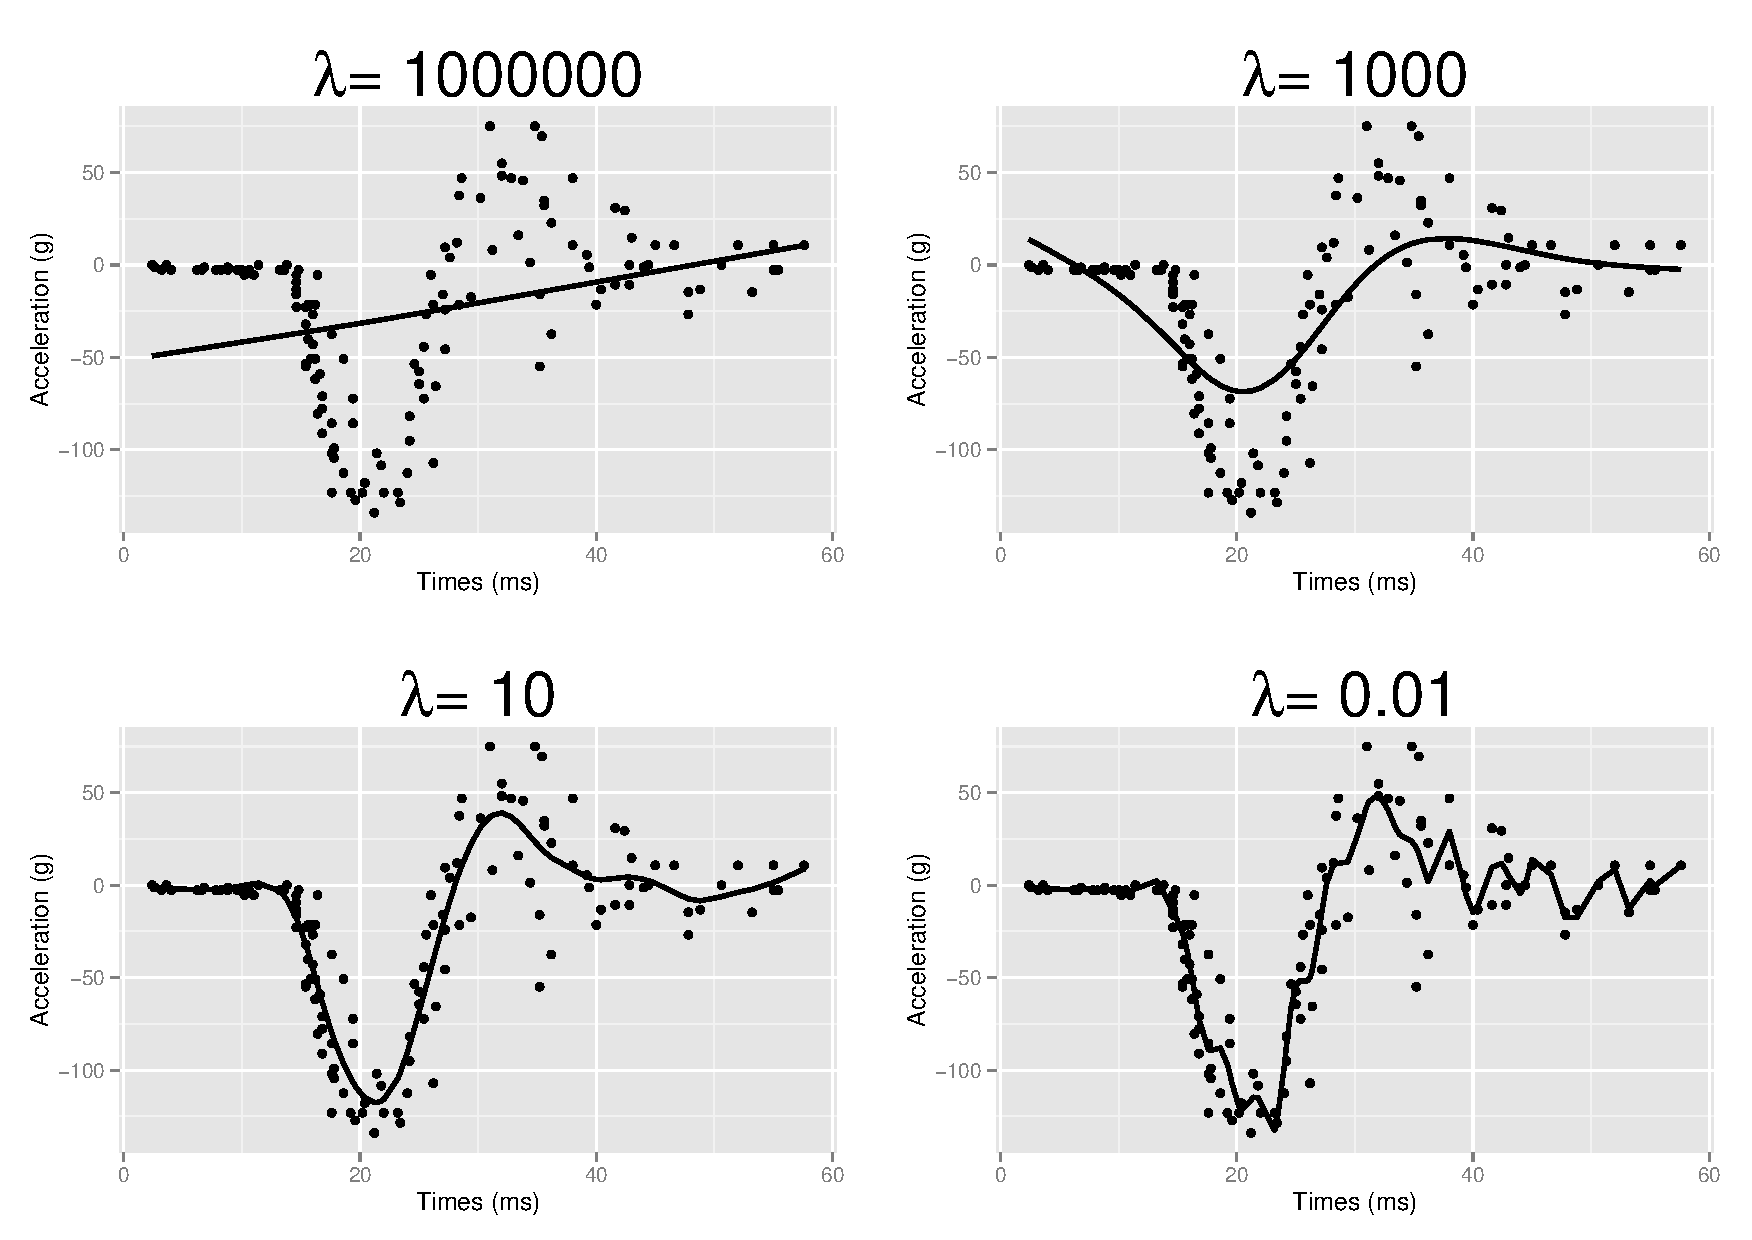
\includegraphics[height=10.5cm, width=1.05\textwidth]{Figures/LS_bspline.pdf}
%    \rule{35em}{0.5pt}
  \caption[\textit{Penalized Least Square} method using B-Splines]{\textit{Penalized Least Square} method using B-Splines on the \texttt{Motorcycle Data} with different values for the smoothing parameter}
  \label{fig:four_plots}
\end{figure}
\clearpage

%---------------------------------------------------------------------------------------
%	SECTION 4
%---------------------------------------------------------------------------------------
\FloatBarrier
\section{Model Selection}\label{section:model_selection}
The task of statistical model selection is to choose a family of distributions among a possible set of families, which is the best approximation of reality manifested in the observed data \citep{Rao2001}.

\subsection{Generalized Cross-Validation (GCV)}\label{GCV}

A measure that is popular in the spline smoothing literature is the \textit{Generalized Cross-Validation }(GCV) developed by \cite{Craven1979}. This data-driven method helps to estimate the smoothing parameter, $\lambda$, which controls the trade-off between the fit of the data and the variability in the function. It is defined to be:

\begin{align}\label{gcv}
GCV(\lambda)&=\dfrac{J^{-1}\text{RSS}}{\left[J^{-1}trace(\mathbb{I}_{J}-\bm{S_{\lambda,\phi}})\right]^{2}} \nonumber \\
            &=\left(\dfrac{J}{J-df(\lambda)}\right)\left(\dfrac{\text{RSS}}{J-df(\lambda)}\right),
\end{align}

where $df(\lambda)=trace(\mathbf{S_{\lambda,\phi}})$. \cite{olberd:ramsay} refer to the quantity in formula \eqref{gcv} as the \textit{"twice-discounted mean squared error measure''}. The minimization of GCV with respect to $\lambda$ involves trying a large set of values of $\lambda$. The GCV criterion can be expressed as:
\begin{equation}
GCV(\lambda)=\dfrac{J\times trace\left\{\bm{Y}^T_i\left[\mathbb{I}_{J}-\bm{S_{\lambda,\phi}}\right]^{-2}\bm{Y}_i\right\}}{\left\{trace\left[\mathbb{I}_{J}-\bm{S_{\lambda,\phi}}\right]\right\}^{2}},
\end{equation}

with $\mathbf{Y}_i$ be the $J \times 1$ vector of observed functional values, $\mathbf{\Phi}$ the $J \times K$ matrix of basis functions and the \textit{hat} matrix $\bm{S}_{\phi,\lambda}$ which is $J \times J$ matrix. With respect to the values of the smoothing parameter $\lambda_i$, the selected values of $\hat{\lambda}_i$ that minimize the \textit{Generalized Cross-Validation} value is the optimal value.\\
\clearpage
\subsubsection*{Numerical Example: Finding the optimal $\lambda$ using GCV}
Consider the \texttt{Motorcycle Data} smoothed using a \textit{Penalized Maximum Likelihood} method as explained in equation \eqref{penalized_likelihood}. Table~\ref{table:gcv_penls} shows the values of GCV that are derived from the $\text{log}_{10} (\lambda)$'s ranging from $-4.1$ to $-3.95$ 
\begin{table}[ht]
\caption[Minimizing the GCV yielding the optimal $\hat{\lambda}$ using \textit{Penalized Maximum Likelihood} method]{$\text{log}_{10} (\lambda)$ against GCV($\lambda$) smoothing the \texttt{Motorcycle Data}} 
\centering % used for centering table
\begin{tabular}{c c } % centered columns (4 columns)
\hline\hline %inserts double horizontal lines
&\\[-2ex]
$\text{log}_{10} (\lambda)$ & GCV($\lambda$) \\ [0.5ex] % inserts table
%heading
\hline\hline 
-4.1	&	567.6346763	\\
-4.09	&	567.6130784	\\
\textbf{-4.08}	&	\textbf{567.6067192}	\\
-4.07	&	567.616065	\\
-4.06	&	567.6415955	\\
-4.05	&	567.6838038	\\
-4.04	&	567.7431973	\\
-4.03	&	567.820297	\\
-4.02	&	567.9156388	\\
-4.01	&	568.0297766	\\
-4	&	568.1632693	\\
-3.99	&	568.3167001	\\
-3.98	&	568.4906646	\\
-3.97	&	568.6857742	\\
-3.96	&	568.902656	\\
-3.95	&	569.1419531	\\
 [0.25ex] % [1ex] adds vertical space
\hline %inserts single line
\end{tabular}
\label{table:gcv_penls} % is used to refer this table in the text
\end{table}
The optimal value for the smoothing parameteris at $\hat{\lambda} = 10^{-4.08}$. Figure~\ref{fig:gcv_plot} outputs: \textbf{(a)} the progression of the GCV-values as the $\text{log}_{10} (\lambda)$'s change with the red line showing the point where the GCV is at its lowest; \textbf{(b)} the smooth curve following the pattern of the \texttt{Motorcycle Data} using B-splines basis functions with $K = 40$ and $\hat{\lambda} = 8.317638 \times 10^{-5}$ as the smoothing parameter. Note that in this case $\hat{\sigma}^2 = 2116.593$.
\begin{figure}[th]
  %\centering
    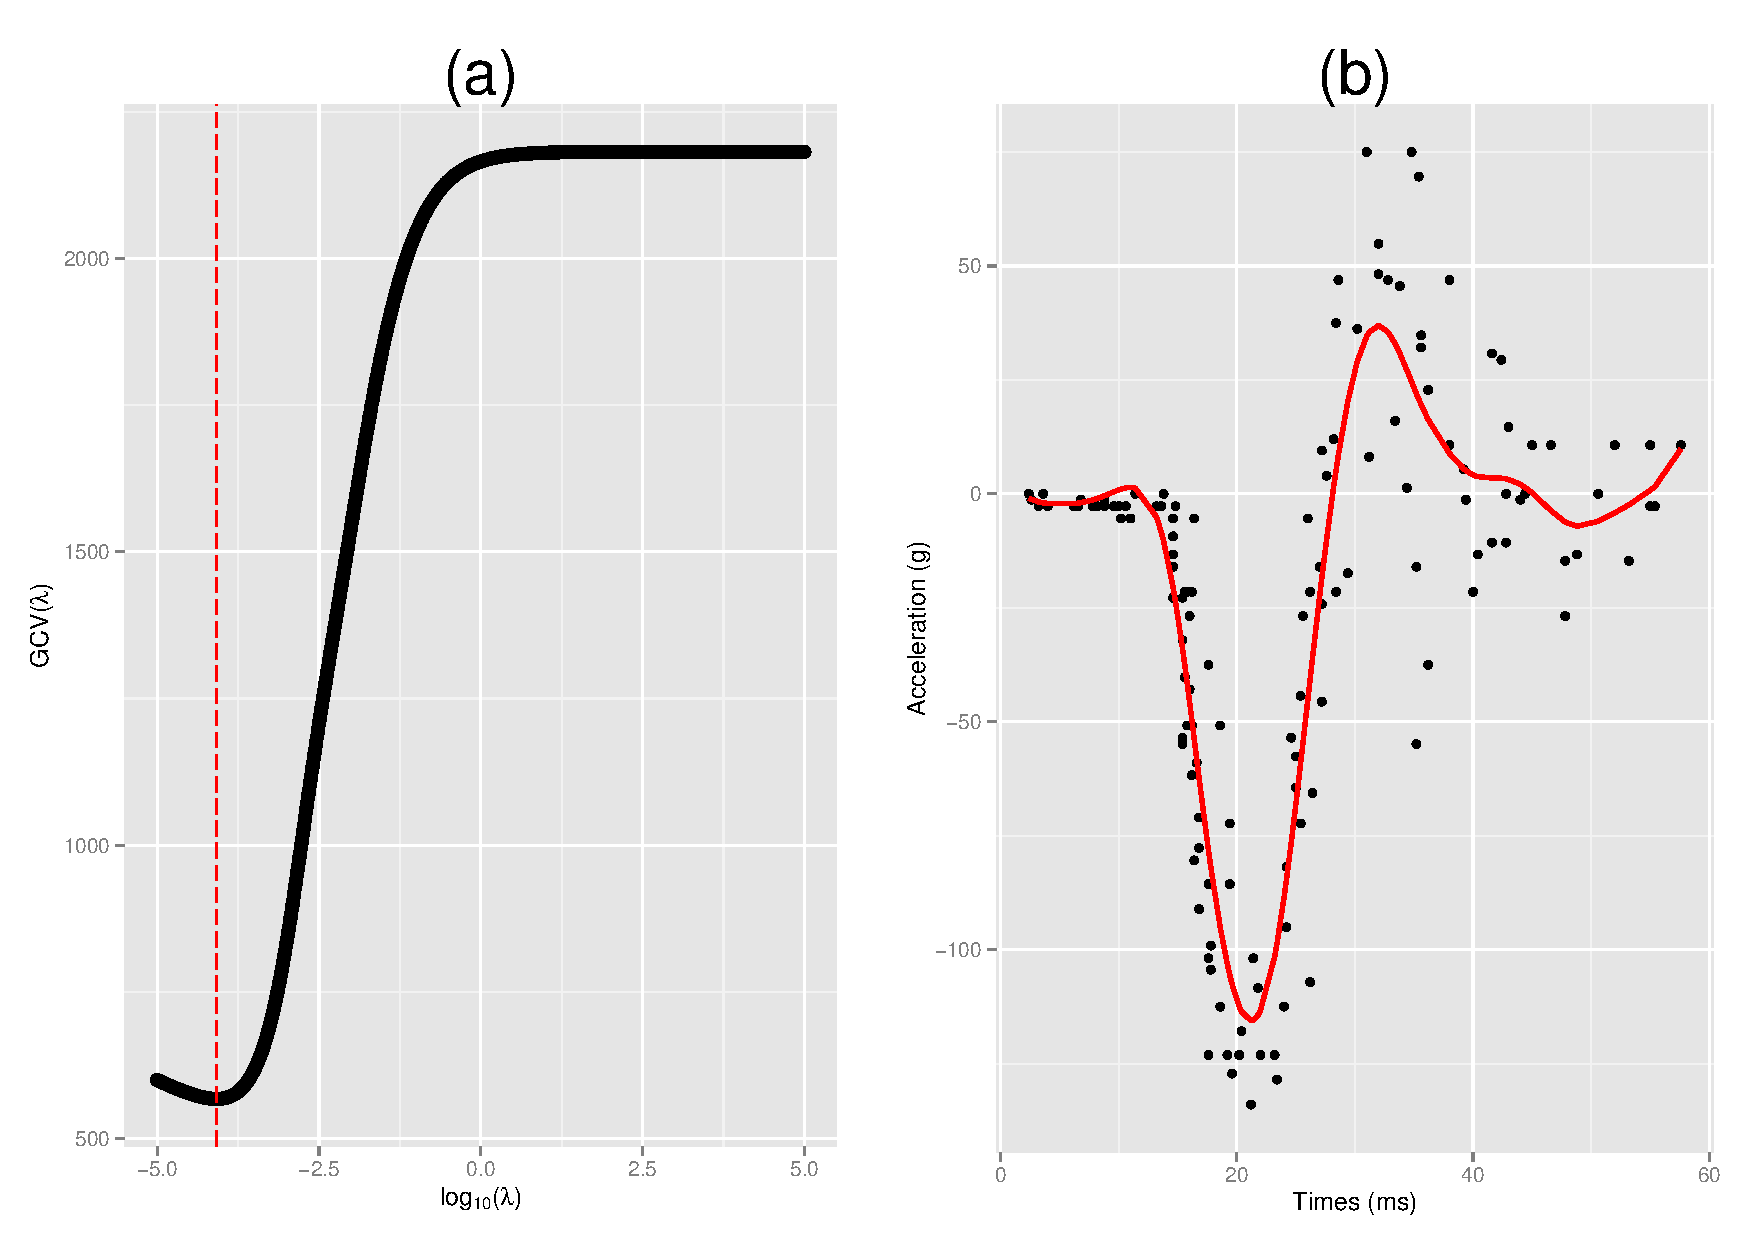
\includegraphics[height=10.5cm, width=1.1\textwidth]{Figures/Rplot_gcv.pdf}
  \caption[\textit{Penalized Maximum Likelihood} method using B-Splines]{\textbf{(a)} $\text{log}_{10} (\lambda)$ against GCV($\lambda$; \textbf{(b)} \texttt{Motorcycle Data} smoothed using \textit{B-Splines Basis} functions with $K = 40$ and GCV criterion yielding $\hat{\lambda} = 10^{-4.08}$ }
  \label{fig:gcv_plot}
\end{figure}
\clearpage

\subsection{Generalized Information Criteria (GIC)}\label{GIC}
First introduced by \cite{Konishi1996}, the GIC can be applied to evaluate statistical models constructed by various types of estimation procedures, more specifically the models estimated by maximum penalized log-likelihood procedures.

Let $G(Y)$ be the true distribution function with density $g(Y)$ that generated data, and let $\hat{G}(Y)$ be the empirical distribution function based on $J$ observations, $\bm{Y}_i = (Y_{i1},Y_{i2},\dots,Y_{iJ})^T$, drawn from $G(Y)$.  Let $\bm{\hat{\theta}}_{GIC}$ be the estimator that maximizes the penalized log-likelihood function \eqref{penalized_likelihood}. It is clear that the estimator $\bm{\hat{\theta}}_{GIC}$ is given as the solution to the following equation:

\begin{equation}
\sum_{j=1}^{J} \bm{\psi}_{GIC}(Y_{.j},\bm{\theta}) = 0,
\end{equation} 
where
\begin{equation}
\bm{\psi}_{GIC}(Y_{.j},\bm{\theta}) = \frac{\partial}{\partial \bm{\theta}} \left\{ \text{log}f(Y_{.j}|t_{.j};\bm{\theta})-\frac{\lambda_i}{2} \bm{c}^T \bm{\Omega} \bm{c} \right\}
\end{equation}
An information criterion for the model $f(Y|\bm{t};\bm{\hat{\theta}}_{GIC})$ with $\bm{\hat{\theta}}_{GIC}$ obtained by maximizing \eqref{penalized_likelihood} is given by:

\begin{equation}
\text{GIC}_{PML} = -2\sum_{j=1}^{J}\text{log}f(Y_{.j}|t_{.j};\bm{\hat{\theta}}_{GIC}) + 2\text{tr}\left\{\bm{R}(\bm{\psi}_{GIC},\hat{G})^{-1} \bm{Q}(\bm{\psi}_{GIC},\hat{G})\right\},
\end{equation}

where $\bm{R}(\bm{\psi}_{GIC},\hat{G})$ and $\bm{Q}(\bm{\psi}_{GIC},\hat{G})$ are $(K+1) \times (K+1)$ matrices given by:

\begin{align}\label{R_Q_eq}
\bm{R}(\bm{\psi}_{GIC},\hat{G})&=-\dfrac{1}{J}\sum_{j=1}^{J}\frac{\partial \bm{\psi}_{MP}(Y_{.j},\bm{\theta})^T}{\partial \bm{\theta}}\bigg|_{\bm{\hat{\theta}} = \bm{\hat{\theta}}_{GIC}}, \\
\bm{Q}(\bm{\psi}_{GIC},\hat{G})&=-\frac{1}{J}\sum_{j=1}^{J}\bm{\psi}(Y_{.j},\bm{\theta})\dfrac{\partial \text{log}f(Y_{.j}|t_{.j};\bm{\theta})}{\partial \bm{\theta}}\bigg|_{\bm{\hat{\theta}} = \bm{\hat{\theta}}_{GIC}}.
\end{align}

By setting $\text{\textit{l}}_j(\bm{\theta})=\text{log}f(Y_{ij}|t_{ij};\bm{\theta})$ (as in equation~\eqref{f_y}), its first and second partial derivatives with respect to $\bm{\theta} = \left(\bm{c}_i^T,\sigma_i^2\right)^T$ are given by:
\begin{align}
\dfrac{\partial l_j(\bm{\theta})}{\partial \sigma_i^2}&=-\dfrac{1}{2\sigma^2_i}+\dfrac{1}{2\sigma^4_i}\left\{Y_{ij}-\bm{c}_i^T\bm{\phi}(t_{ij})\right\}^2,\nonumber \\
\dfrac{\partial l_j(\bm{\theta})}{\partial \bm{c}_i}&=\dfrac{1}{\sigma_i^2}\left\{Y_{ij}-\bm{c}_i^T\bm{\phi}(t_{ij})\right\}\bm{\phi}(t_{ij}),
\end{align}

and
\begin{align}
\dfrac{\partial^2 l_j(\bm{\theta})}{\partial \sigma_i^2\partial \sigma_i^2}&=-\dfrac{1}{2\sigma^4_i}-\dfrac{1}{\sigma^6_i}\left\{Y_{ij}-\bm{c}_i^T\bm{\phi}(t_{ij})\right\}^2,\nonumber \\
\dfrac{\partial^2 l_j(\bm{\theta})}{\partial \bm{c}_i\partial \bm{c}^T_i}&=-\dfrac{1}{\sigma_i^2}\bm{\phi}(t_{ij})\bm{\phi}(t_{ij})^T, \nonumber \\
\dfrac{\partial^2 l_j(\bm{\theta})}{\partial \sigma_i^2\partial \bm{c}_i}&=-\dfrac{1}{\sigma_i^4}\left\{Y_{ij}-\bm{c}_i^T\bm{\phi}(t_{ij})\right\}\bm{\phi}(t_{ij}).
\end{align}

The matrices $\bm{R}(.)$ \& $\bm{Q}(.)$ can be derived as follows:

\begin{center}
$\dfrac{\partial \bm{\psi}_{MP}(Y_{.j},\bm{\theta})^T}{\partial \bm{\theta}}=\def\arraystretch{2}
\begin{bmatrix}
\dfrac{\partial^2 l_j(\bm{\theta})}{\partial \bm{c}_i \partial \bm{c}_i^T} - \lambda_i \bm{\Omega} & \dfrac{\partial^2 l_j(\bm{\theta})}{\partial \bm{c}_i \partial \sigma_i^2} \\
\dfrac{\partial^2 l_j(\bm{\theta})}{ \partial \sigma_i^2 \partial \bm{c}_i} & \dfrac{\partial^2 l_j(\bm{\theta})}{\partial \sigma_i^2 \partial \sigma_i^2}
\end{bmatrix}$,
\end{center}

$\bm{\psi}_{MP}(Y_{.j},\bm{\theta})\dfrac{\partial \text{log}f(Y_{.j}|t_{.j};\bm{\theta})}{\partial \bm{\theta}}$
\begin{center}
=\def\arraystretch{2}
\begin{bmatrix}
\dfrac{\partial l_j(\bm{\theta})}{\partial \bm{c}_i}\dfrac{\partial l_j(\bm{\theta})}{\partial \bm{c}_i^T} - \lambda_i \bm{\Omega}\bm{c}_i\dfrac{\partial l_j(\bm{\theta})}{\partial \bm{c}_i^T} & \dfrac{\partial l_j(\bm{\theta})}{\partial \bm{c}_i}\dfrac{\partial l_j(\bm{\theta})}{\partial \sigma_i^2} - \lambda_i \bm{\Omega}\bm{c}_i\dfrac{\partial l_j(\bm{\theta})}{\partial \sigma_i^2} \\
\dfrac{\partial l_j(\bm{\theta})}{\partial \sigma_i^2}\dfrac{\partial l_j(\bm{\theta})}{\partial \bm{c}_i^T} & \left\{\dfrac{\partial l_j(\bm{\theta})}{\partial \sigma_i^2}\right\}^2
\end{bmatrix},
\end{center}

therefore:

\begin{center}
$\bm{R}(\bm{\psi}_{GIC},\hat{G})=\dfrac{1}{J\sigma_i^2}\def\arraystretch{2}
\begin{bmatrix}
\bm{\Phi}^T\bm{\Phi}+J \lambda_i \hat{\sigma}^2_i \bm{\Omega} & \dfrac{1}{\hat{\sigma}^2_i}\bm{\Phi}^T \bm{\Lambda}_i \bm{\big{1}}_J \\
\dfrac{1}{\hat{\sigma}^2_i}\bm{\big{1}}_J^T \bm{\Lambda}_i \bm{\Phi} & \dfrac{J}{2\sigma_i^2}
\end{bmatrix}$,
\end{center}

\begin{center}
$\bm{Q}(\bm{\psi}_{GIC},\hat{G})=\dfrac{1}{J\sigma_i^2}\def\arraystretch{2}
\begin{bmatrix}
\dfrac{1}{2\sigma_i^2}\bm{\Phi}^T\bm{\Lambda}_i^2\bm{\Phi} - \lambda_i \bm{\Omega} \bm{c}_i \bm{\big{1}}_J^T \bm{\Lambda}_i \bm{\Phi} & \dfrac{1}{2\hat{\sigma}^4_i}\bm{\Phi}^T \bm{\Lambda}_i^3 \bm{\big{1}}_J - \dfrac{1}{2\hat{\sigma}^2_i}\bm{\Phi}^T \bm{\Lambda}_i \bm{\big{1}}_J \\
\dfrac{1}{2\hat{\sigma}^4_i}\bm{\big{1}}_J^T \bm{\Lambda}_i^3 \bm{\Phi}- \dfrac{1}{2\hat{\sigma}^4_i}\bm{\big{1}}_J^T \bm{\Lambda}_i \bm{\Phi} & \dfrac{1}{4\hat{\sigma}^6_i}\bm{\big{1}}_J^T \bm{\Lambda}_i^4 \bm{\big{1}}_J-\dfrac{J}{4\sigma_i^2}
\end{bmatrix}$,
\end{center}
where $\bm{\big{1}}_J = (1,1,\dots,1)^T$ is a $J$-dimensional vector of 1's, and $\bm{\Lambda}$ is a $J \times J$ diagonal matrix defined by

\begin{equation*}
\bm{\Lambda}_i = \text{diag} \left[Y_{i1} - \bm{\hat{c}}_i^T\bm{\phi}(t_{i1}),Y_{i2} - \bm{\hat{c}}_i^T\bm{\phi}(t_{i2}),\dots,Y_{iJ} - \bm{\hat{c}}^T_i\bm{\phi}(t_{iJ})\right]
\end{equation*}

\subsubsection*{Numerical Example: Finding the optimal $\lambda$ using GIC}
Consider the \texttt{Motorcycle Data} smoothed using the \textit{Penalized Maximum Likelihood} method as explained in equation \eqref{penalized_likelihood}. Table~\ref{table:gic_penml} shows the values of GIC that are derived from the $\text{log}_{10} (\lambda)$'s ranging from $-4.3$ to $-4.1$ 
\begin{table}[ht]
\caption[Minimizing the GIC yields to the optimal $\hat{\lambda}$ using \textit{Penalized Maximum Likelihood} method]{$\text{log}_{10} (\lambda)$ against GIC($\lambda$) smoothing the \texttt{Motorcycle Data}} 
\centering % used for centering table
\begin{tabular}{c c } % centered columns (4 columns)
\hline\hline %inserts double horizontal lines
&\\[-2ex]
$\text{log}_{10} (\lambda)$ & GIC($\lambda$) \\ [0.5ex] % inserts table
%heading
\hline\hline 
-4.3	&	1216.693	\\
-4.29	&	1216.679	\\
-4.28	&	1216.666	\\
-4.27	&	1216.655	\\
-4.26	&	1216.646	\\
-4.25	&	1216.639	\\
-4.24	&	1216.633	\\
-4.23	&	1216.630	\\
\textbf{-4.22}	&	\textbf{1216.629}	\\
-4.21	&	1216.630	\\
-4.2	&	1216.633	\\
-4.19	&	1216.638	\\
-4.18	&	1216.646	\\
-4.17	&	1216.656	\\
-4.16	&	1216.669	\\
-4.15	&	1216.684	\\
-4.14	&	1216.702	\\
-4.13	&	1216.723	\\
 [0.25ex] % [1ex] adds vertical space
\hline %inserts single line
\end{tabular}
\label{table:gic_penml} % is used to refer this table in the text
\end{table}
The optimal value for the smoothing parameter is at $\hat{\lambda} = 10^{-4.22}$. Figure~\ref{fig:gic_plot} outputs: \textbf{(a)} the progression of the GIC-values as the $\text{log}_{10} (\lambda)$'s change with the red line showing the point where the GIC is at its lowest; \textbf{(b)} the smooth curve following the pattern of the \texttt{Motorcycle Data} using \textit{B-Splines Basis} functions with $K = 40$ and $\hat{\lambda} = 6.025596 \times 10^{-5}$ as the smoothing parameter. It is important to note that $\hat{\sigma}^2 = 462.5911$.

\begin{figure}[th]
  %\centering
    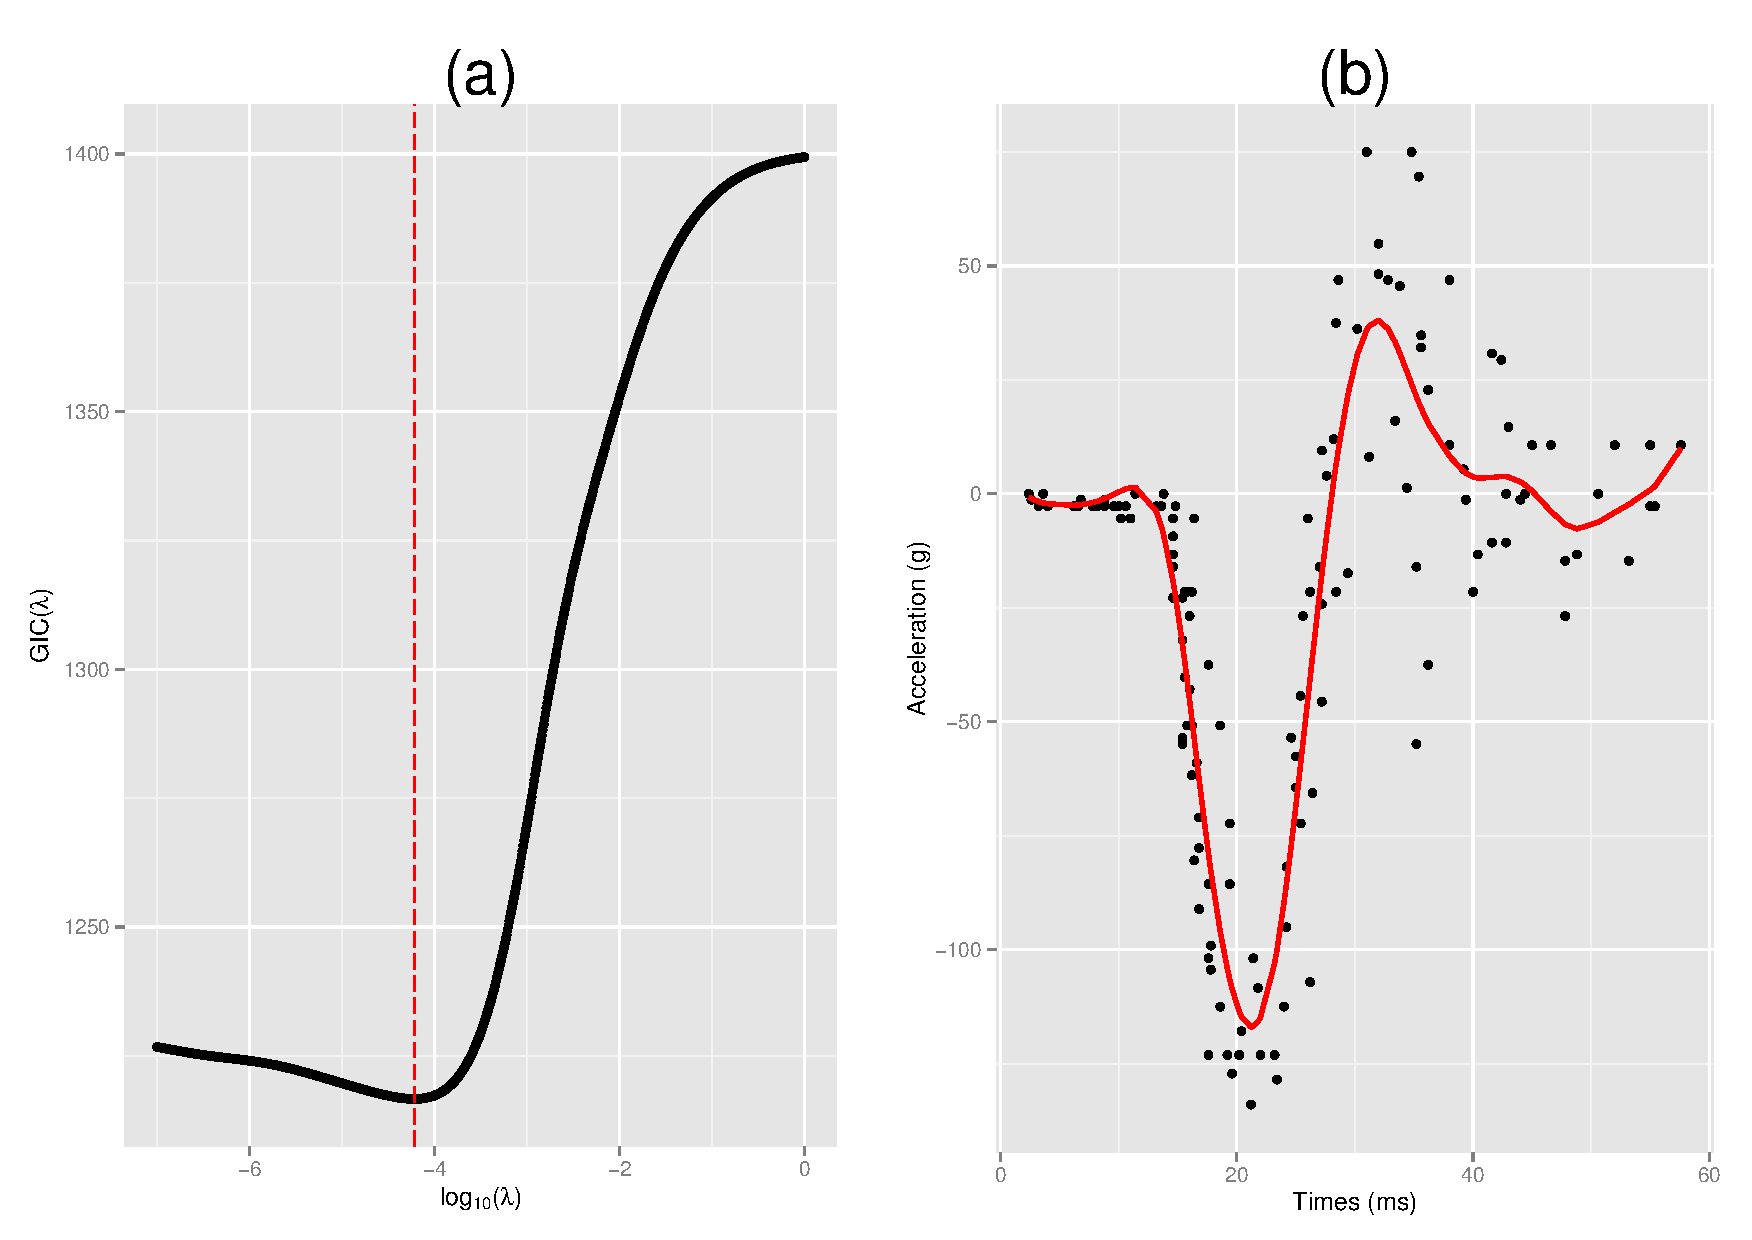
\includegraphics[height=10.5cm, width=1.1\textwidth]{Figures/Rplot_gic.pdf}
  \caption[\textit{Penalized Maximum Likelihood} method evaluated using GIC]{\textbf{(a)} $\text{log}_{10} (\lambda)$ against GIC($\lambda$); \textbf{(b)} \texttt{Motorcycle Data} smoothed using\textit{B-Splines Basis} functions with $K = 40$ and GIC criterion yielding $\hat{\lambda} = 10^{-4.22}\text{ }\&\text{ }\hat{\sigma}^2 = 462.5911$ }
  \label{fig:gic_plot}
\end{figure}
%The minimization of \textit{GIC} with respect to the model parameters will involve trying to inspect a large number of values where at least one of these values will be the optimal value.

\subsection{Modified Akaike Information Criteria (mAIC)}\label{mAIC}
The Akaike's information criteria (1973) was derived as an estimator of the \cite{kullback1951} information from the predictive point of view. It is given by:

\begin{equation}\label{aic}
-2 l(\bm{Y}_i|\bm{\hat{\theta}}_{ML}) + 2(\text{number of parameters})
\end{equation} 

where $l(\bm{\hat{\theta}}_{ML})$ is the log-likelihood of a model estimated by the \textit{Maximum Likelihood} and the ``number of parameters'' is a measure of complexity of the model. However, in nonlinear modelling, the ``number of parameters'' is not an appropriate measure of model complexity since it may depend on both the regularization term and the observed data. \cite{Fujikoshi1997} considered using the trace \textit{smoother operator} (see equations \eqref{project_op1} \& \eqref{project_op2}) as an approximation to the effective ``number of parameters''. By replacing the last term in \eqref{aic} by $\text{tr }(S_{\lambda_i})$, the \textit{mAIC} is given by:

\begin{equation}
\text{mAIC} = J \text{ log}(2 \pi \hat{\sigma}_i^2) + J + 2\text{ tr}(S_{\lambda_i})
\end{equation}

\subsubsection*{Numerical Example: Finding the optimal $\lambda$ using mAIC}
The \texttt{Motorcycle Data} is smoothed using the \textit{penalized maximum likelihood}. Table~\ref{table:maic_penml} is showing the values of mAIC that are derived from the $\text{log}_{10} (\lambda)$'s ranging from $-4.2$ to $-4.05$. 
\begin{table}[ht]
\caption[Minimizing the mAIC yields to the optimal $\hat{\lambda}$ using \textit{Penalized Maximum Likelihood} method]{$\text{log}_{10} (\lambda)$ against mAIC($\lambda$) smoothing the \texttt{Motorcycle Data}} 
\centering % used for centering table
\begin{tabular}{c c } % centered columns (4 columns)
\hline\hline %inserts double horizontal lines
&\\[-2ex]
$\text{log}_{10} (\lambda)$ & mAIC($\lambda$) \\ [0.5ex] % inserts table
%heading
\hline\hline 
-4.2	&	1216.633	\\
-4.19	&	1216.638	\\
-4.18	&	1216.646	\\
-4.17	&	1216.656	\\
-4.16	&	1216.669	\\
-4.15	&	1216.684	\\
-4.14	&	1216.702	\\
-4.13	&	1216.723	\\
\textbf{-4.12}	&	\textbf{1216.747}	\\
-4.11	&	1216.774	\\
-4.1	&	1216.803	\\
-4.09	&	1216.836	\\
-4.08	&	1216.873	\\
-4.07	&	1216.913	\\
-4.06	&	1216.956	\\
-4.05	&	1217.003	\\
 [0.25ex] % [1ex] adds vertical space
\hline %inserts single line
\end{tabular}
\label{table:maic_penml} % is used to refer this table in the text
\end{table}
The optimal value for the smoothing parameter is at $\hat{\lambda} = 10^{-4.12}$. Figure~\ref{fig:maic_plot} outputs: \textbf{(a)} the progression of the mAIC-values as the $\text{log}_{10} (\lambda)$'s change with the red line showing the point where the mAIC is at its lowest; \textbf{(b)} the smooth curve following the pattern of the \texttt{Motorcycle Data} using \textit{B-Splines Basis} functions with $K = 40$ and $\hat{\lambda} = 7.585776 \times 10^{-5}$ as the smoothing parameter. Note that$\hat{\sigma}^2 = 466.3463$

\begin{figure}[th]
  %\centering
    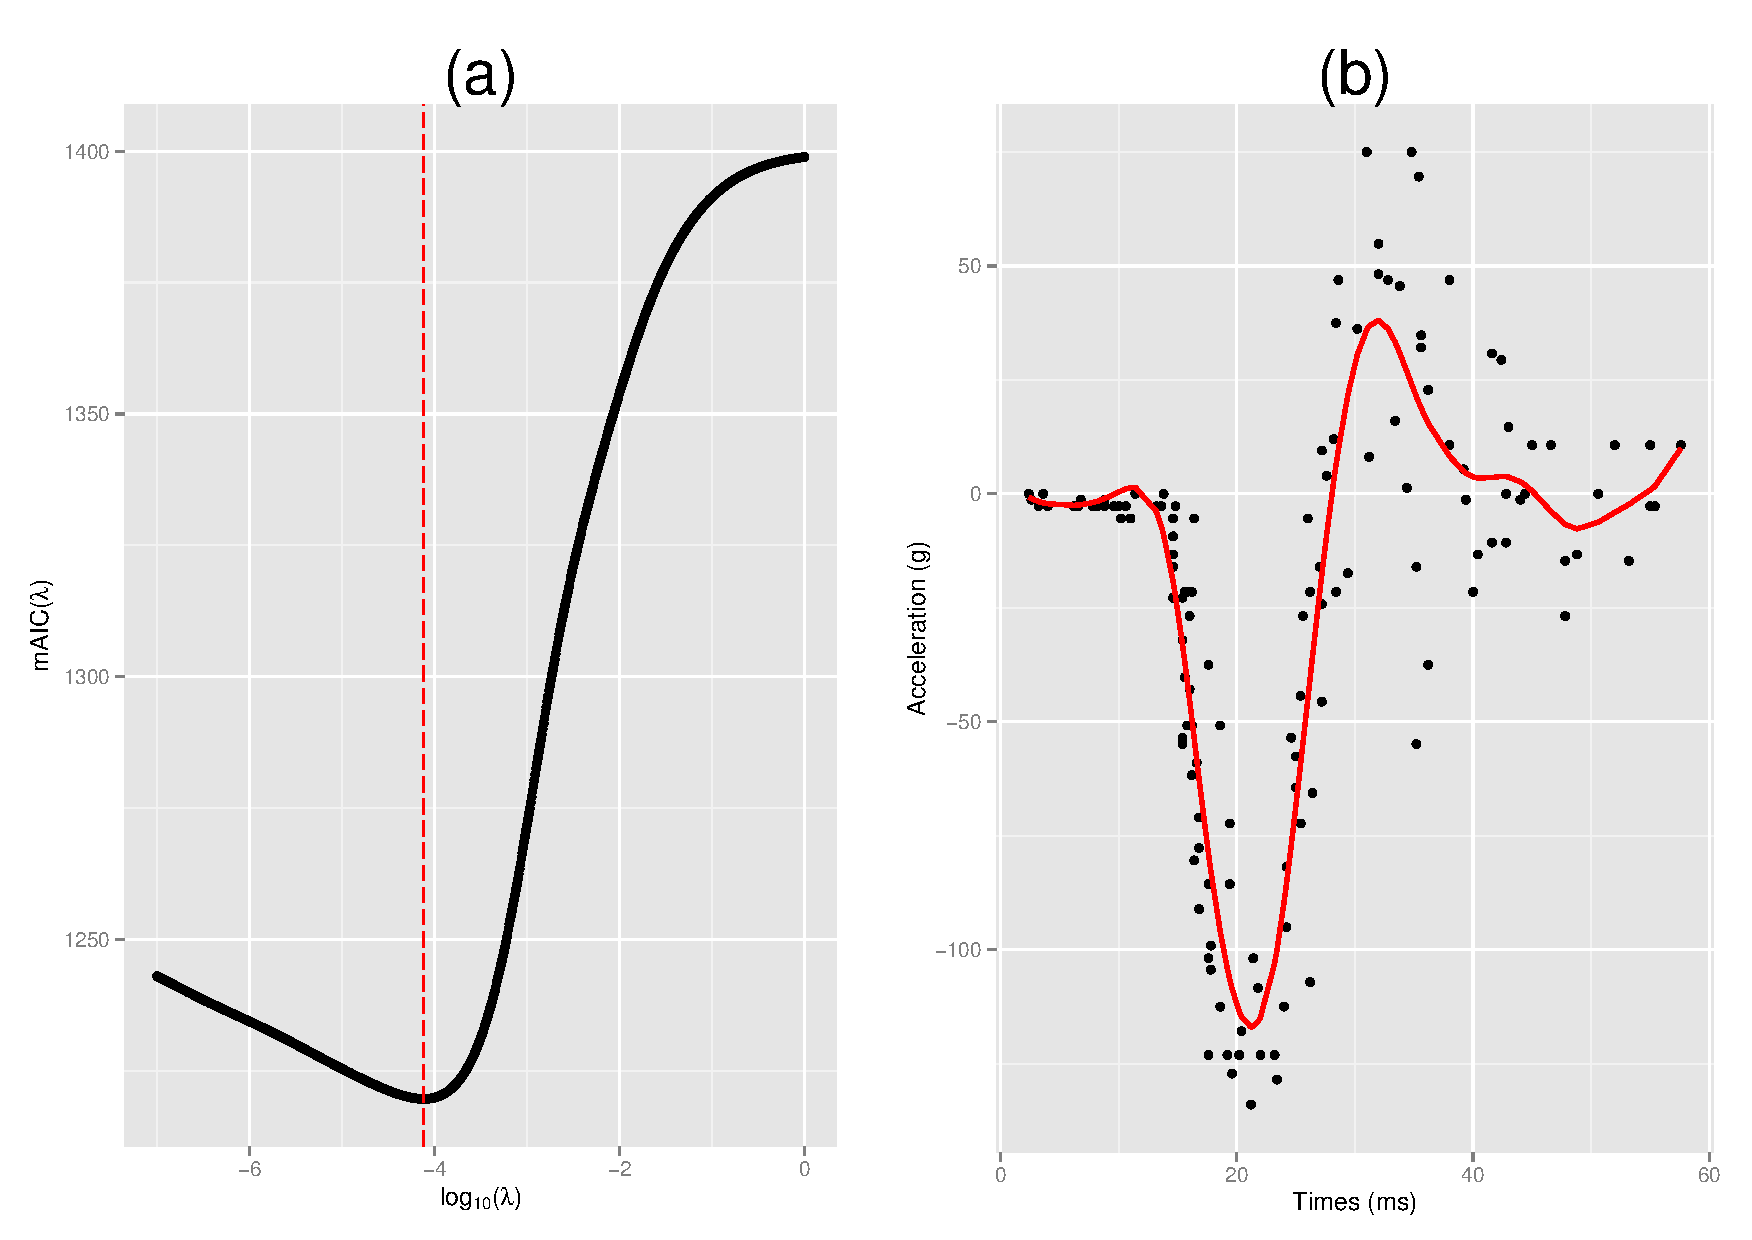
\includegraphics[height=10.5cm, width=1.1\textwidth]{Figures/Rplot_maic.pdf}
  \caption[\textit{Penalized Maximum Likelihood} method evaluated using mAIC]{\textbf{(a)} $\text{log}_{10} (\lambda)$ against mAIC($\lambda$); \textbf{(b)} \texttt{Motorcycle Data} smoothed using B-splines basis functions with $K = 40$ and mAIC criterion yielding $\hat{\lambda} = 10^{-4.12}\text{ }\&\text{ }\hat{\sigma}^2 = 466.3463$ }
  \label{fig:maic_plot}
\end{figure}
\clearpage

\subsection{Generalized Bayesian Information Criteria (GBIC)}\label{GBIC} 
Derived from the well known \textit{Bayesian Information Criteria} (BIC), it is a model selection criterion used to evaluate models fitted by the \textit{Penalized Maximum Likelihood} method or the method of \textit{Regularization}. \cite{Konishi2004} derived this criterion in order to estimate the smoothing parameters as well as other parameters such as the number of basis functions.\\
Suppose that the suitable model is constructed by maximizing equation~\eqref{penalized_likelihood} yielding the maximum likelihood estimators for $\bm{c}_i$ and $\sigma^2_i$ (see equation~\ref{solution_eqpen}). Considering $\beta_i = \lambda_i \sigma^2_i$ and subsituting back in equation~\eqref{solution_eqpen}, the \textit{Generalized Bayesian Information Criteria} is given by: 
\begin{eqnarray}
\text{GBIC }&=&(J+K-1)\text{ log}\hat{\sigma}^2_i + J \beta_i\hat{\bm{c}}^T_i \bm{\Omega} \hat{\bm{c}}_i /\hat{\sigma}^2_i + J +(J-3)\text{ log}(2\pi) + 3\text{ log}J \nonumber\\ 
&& + \text{ log} |\bm{Q}_{\beta_i}^{(G)} (\hat{\bm{c}}^T_i,\hat{\sigma}^2_i)| - \text{ log}|\bm{\Omega}|_{+} - (K-1)\text{ log} \beta_i
\end{eqnarray}
where $|\bm{\Omega}| _{+}$ denotes the product of nonzero eigenvalues of $\bm{\Omega}$ and
\begin{center}
$\bm{Q}_{\beta_i}^{(G)} (\hat{\bm{c}}^T_i,\hat{\sigma}^2_i)=\dfrac{1}{J\sigma_i^2}\def\arraystretch{2}
\begin{bmatrix}
\bm{\Phi}^T\bm{\Phi} + J \beta_i \bm{\Omega} & \bm{\Phi}^T \bm{e} / \hat{\sigma}^2_i \\
\bm{e}^T \bm{\Phi} / \hat{\sigma}^2_i & \dfrac{J}{2\sigma_i^2}
\end{bmatrix}$.
\end{center}
Note that $\bm{e}$ is a $J$-dimensional vector given by
\begin{equation*}
\bm{e} = \left[Y_{i1} - \bm{\hat{c}}_i^T\bm{\phi}(t_{i1}),Y_{i2} - \bm{\hat{c}}_i^T\bm{\phi}(t_{i2}),\dots,Y_{iJ} - \bm{\hat{c}}^T_i\bm{\phi}(t_{iJ})\right]^T.
\end{equation*}
For a more extensive derivation of the above result, consult the journal article written by \cite{Konishi1996}.

\subsubsection*{Numerical Example: Finding the optimal $\lambda$ using GBIC}
The \texttt{Motorcycle Data} is smoothed using the \textit{Penalized Maximum Likelihood}. Table~\ref{table:gbic_penml} is showing the values of GBIC that are derived from the $\text{log}_{10} (\lambda)$'s ranging from $-4.3$ to $-4.15$ 
\begin{table}[ht]
\caption[Minimizing the GBIC yields to the optimal $\hat{\lambda}$ using \textit{Penalized Maximum Likelihood} method]{$\text{log}_{10} (\lambda)$ against GBIC($\lambda$) smoothing the \texttt{Motorcycle Data}} 
\centering % used for centering table
\begin{tabular}{c c } % centered columns (4 columns)
\hline\hline %inserts double horizontal lines
&\\[-2ex]
$\text{log}_{10} (\lambda)$ & GBIC($\lambda$) \\ [0.5ex] % inserts table
%heading
\hline\hline 
-4.3	&	1258.324	\\
-4.29	&	1258.288	\\
-4.28	&	1258.257	\\
-4.27	&	1258.232	\\
-4.26	&	1258.213	\\
-4.25	&	1258.200	\\
-4.24	&	1258.193	\\
\textbf{-4.23}	&	\textbf{1258.192}	\\
-4.22	&	1258.196	\\
-4.21	&	1258.208	\\
-4.2	&	1258.225	\\
-4.19	&	1258.249	\\
-4.18	&	1258.279	\\
-4.17	&	1258.315	\\
-4.16	&	1258.358	\\
-4.15	&	1258.408	\\
 [0.25ex] % [1ex] adds vertical space
\hline %inserts single line
\end{tabular}
\label{table:gbic_penml} % is used to refer this table in the text
\end{table}
The optimal value for the smoothing parameter is at $\hat{\lambda} = 10^{-4.23}$. Figure~\ref{fig:gbic_plot} outputs: \textbf{(a)} the progression of the mAIC-values as the $\text{log}_{10} (\lambda)$'s change with the red line showing the point where the mAIC is at its lowest; \textbf{(b)} the smooth curve following the pattern of the \texttt{Motorcycle Data} using \textit{B-Splines Basis} functions with $K = 40$ and $\hat{\lambda} = 5.888437 \times 10^{-5}$ as the smoothing parameter. Note that $\hat{\sigma}^2 = 462.2833$

\begin{figure}[th]
  %\centering
    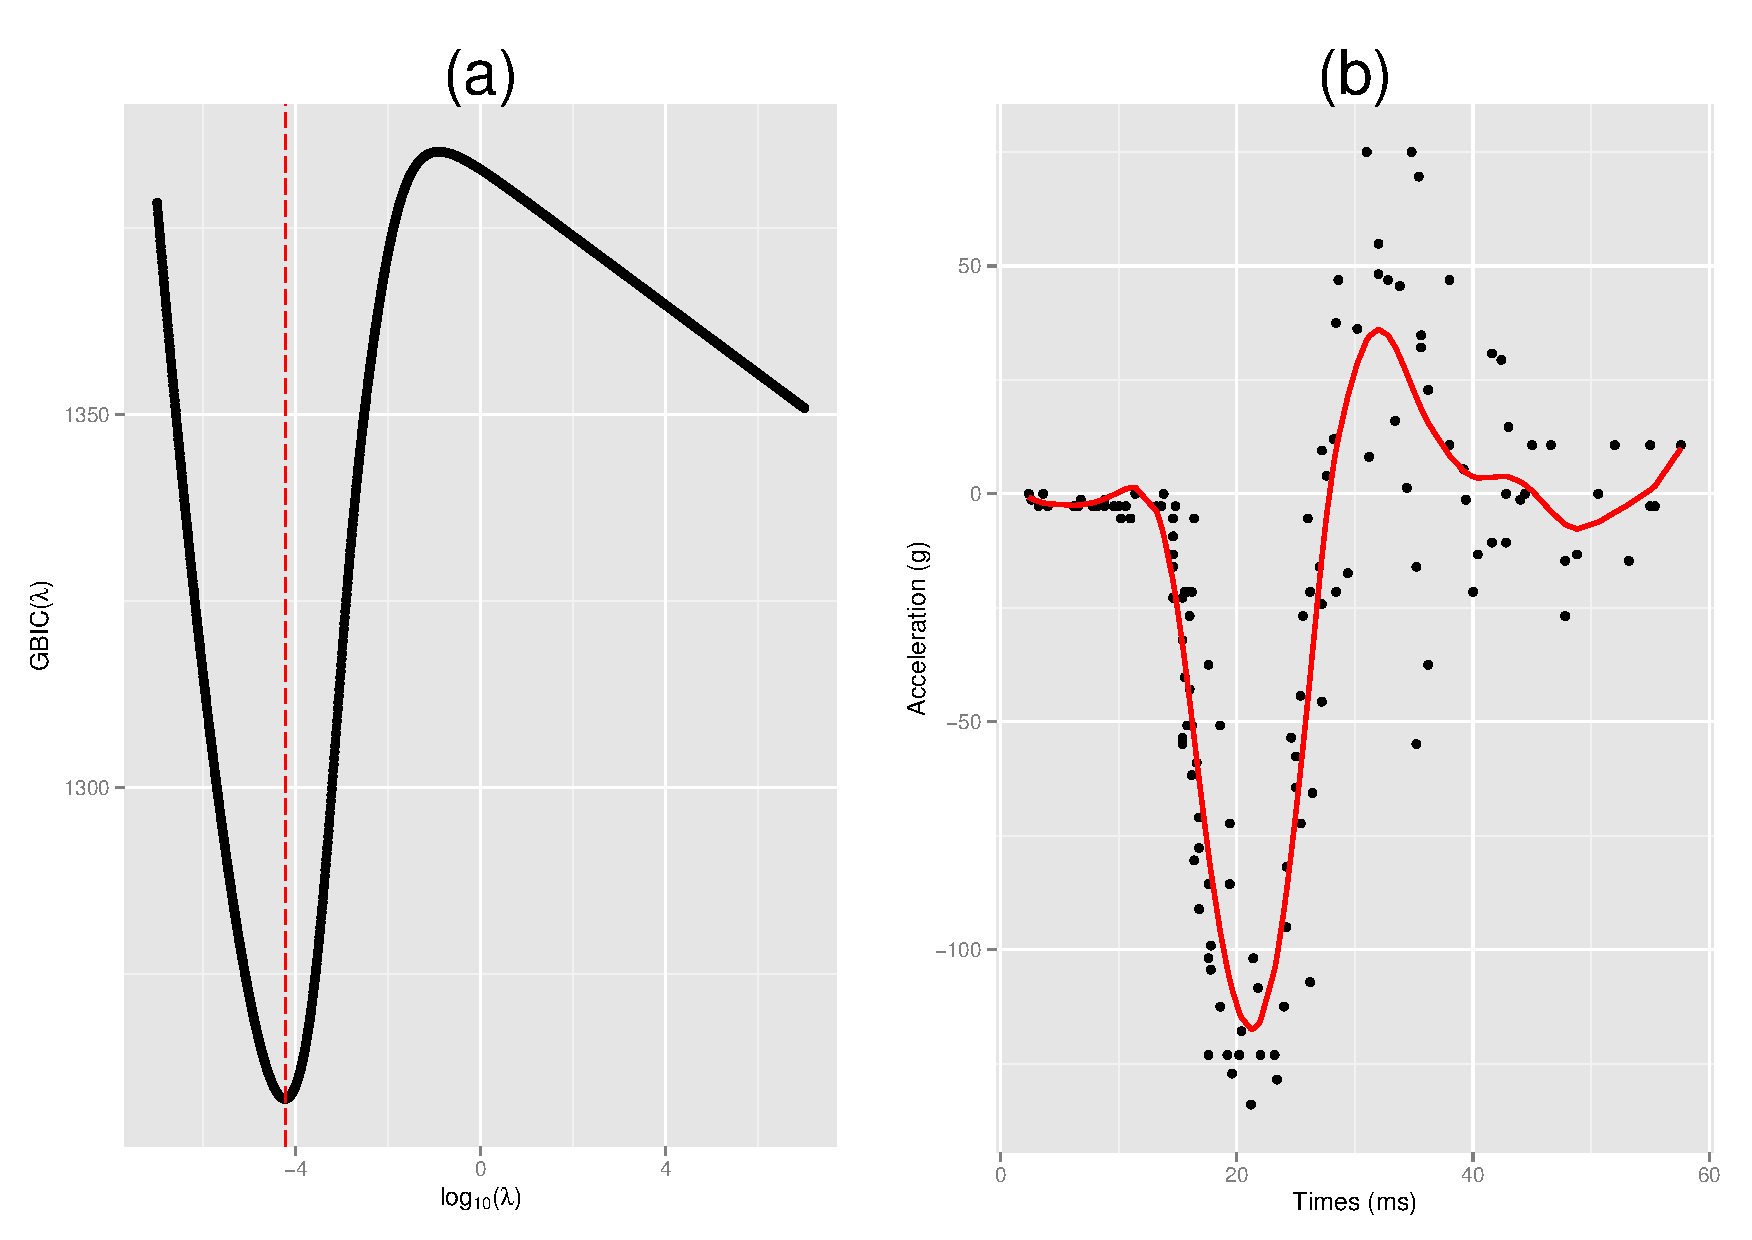
\includegraphics[height=10.5cm, width=1.1\textwidth]{Figures/Rplot_gbic.pdf}
  \caption[\textit{Penalized Maximum Likelihood} method evaluated using GBIC]{\textbf{(a)} $\text{log}_{10} (\lambda)$ against GBIC($\lambda$); \textbf{(b)} \texttt{Motorcycle Data} smoothed using \textit{B-splines} basis functions with $K = 40$ and GBIC criterion yielding $\hat{\lambda} = 10^{-4.23}\text{ }\&\text{ }\hat{\sigma}^2 = 462.2833$ }
  \label{fig:gbic_plot}
\end{figure}
\clearpage

Although the \textit{Generalized Cross-Validation} criterion is widely used for the regularization parameter selection, the computational time is very large and high variability and tendency to undersmooth are not negligible in the analysis of Functional Data \citep{Matsui2009}. Table~\ref{table:summary1} illustrates that argument with a high value for the GCV Mean Square Errors (MSE) as well as its estimated $\hat{\sigma}_{GCV}^2$; it is important to point out that the number of basis functions is the same for all model criteria. 

\begin{table}[ht]
\caption[Summary of the model selection applied on the \texttt{Motorcycle Data} with $K = 40$]{Summary of the model selection applied on the \texttt{Motorcycle Data} smoothed using B-splines basis functions with $K = 40$}
\centering % used for centering table
\begin{tabular}{c @{\hspace{0.2cm}\vrule width 2pt\hspace{0.2cm}} c c c } % centered columns (4 columns)
\hline %inserts double horizontal lines
\multicolumn{1}{c}{} & & &  \\[-2ex]
 \multicolumn{1}{c}{}& $\text{log}_{10} (\hat{\lambda})$ & $\hat{\sigma}^2$ & MSE \\ [0.5ex] % inserts table
%heading
\noalign{\hrule height 1pt} 
GCV &	-4.08 & \textbf{2116.593}	&	\textbf{468.1117}	\\
GIC &	-4.22 & 462.5911	&	462.5911	\\
mAIC &	-4.12 & 466.3463	&	466.3463	\\
GBIC &	-4.23 & 462.2833	&	462.2833	\\
 [0.25ex] % [1ex] adds vertical space
\hline  %inserts single line
\end{tabular}
\label{table:summary1} % is used to refer this table in the text
\end{table}

\subsection{The optimal number \textit{K} of Basis Functions}
Choosing the optimal number $K$ of basis functions is an important task when converting the discrete observations into Functional Data. The larger $K$ the better the fit to the data, but at the same time the risk of fitting noise or variation that should not be ignored. On the other hand, if $K$ is too small, some important aspects of the smooth function might be disregarded when trying to estimate the function \citep{olberd:ramsay}. One of the main reasons for smoothing is to reduce the influence of noise as well as to capture meaningful regularities on the estimates. The idea of the penalization is to rather overfit the data and then penalize to obtain a bias-variance trade-off. The methods for model selection (mentioned above) may offer some guidance in the choice of the optimal $K$, however for each value of the number of basis functions there is an optimal value for $\hat{\lambda}$ \& $\hat{\sigma}^2$. 
%---------------------------------------------------------------------------------------
%	SECTION 5
%---------------------------------------------------------------------------------------
\clearpage
\section{Functional Descriptive Statistics}
One of the most important parts in data analysis is the exploratory part: Estimating means and standard deviations. Because the functional nature of the data, the associated descriptive statistics are therefore functional.

\subsection{Mean \& Variance functions}
Estimating the \textit{Mean Function} based on discretely sampled noisy observations is one of the most basic problems in Functional Data Analysis. The \textit{Mean Function} is a simple analogue of the classical mean for univariate data. It can be calculated by averaging the functions point-wise across the replications, since Functional Data Analysis sees each curve as a distinct datum itself. The mean function is defined as $\mathbf{\nu}_{\mathcal{X}}(t)=\mathbb{E}(X(t)),\text{ }\forall t \in \mathcal{T}$. The sample mean curve is: 

\begin{equation} \label{eq:functmean}
\bar{X}(t)=\frac{1}{N}(X_{1}(t)+\dots+X_{N}(t)),\text{ }\forall t \in \mathcal{T} 
\end{equation}

where \textit{N} is the number of curves or replications and $X_{i}(t)$ is the \textit{i-th} function evaluated at time \textit{t}. Below is a plot illustrating the concept of \textit{Functional Mean} applied on the \texttt{Canadian Weather} dataset from \cite{olberd:ramsay}. The \textit{Functional Mean} is calculated for five weather stations namely \textit{St.Johns, Halifax, Sydney, Yarmouth \& Charlottville} represented using a \textit{Fourier Basis} expansion with $K = 65$:
\begin{figure}[h]
  \centering
    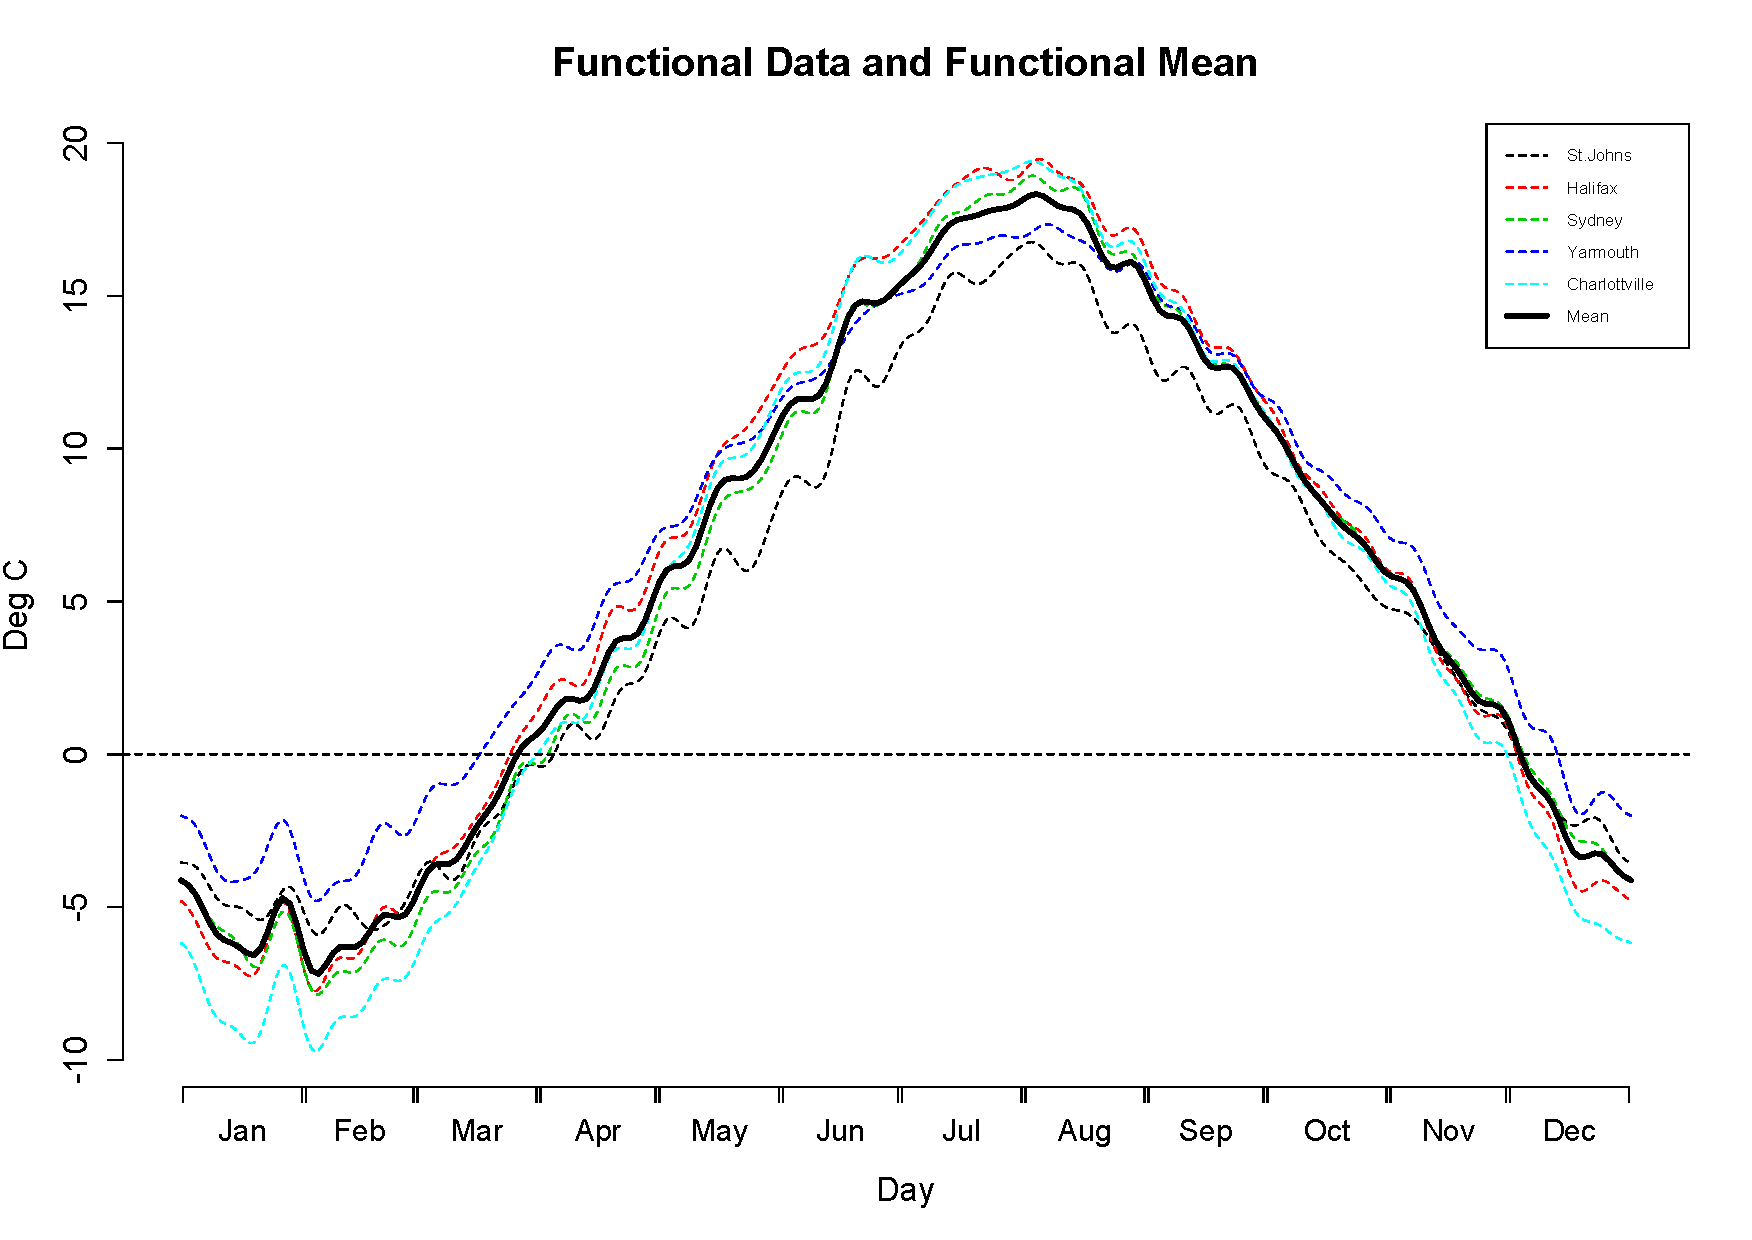
\includegraphics[height=7cm, width=1\textwidth]{Figures/functionalmean1.pdf}
%    \rule{35em}{0.5pt}
  \caption[\textit{Functional Mean} applied on Canadian Weather dataset]{Canadian Weather data: Mean Curve \footnote{I need to introduce a legend on the plot.}.}
  \label{fig:meancurve}
\end{figure}

Likewise, the estimation of the \textit{Functional Variance} is very similar to the classical variance for univariate data. It is defined as $\mathbf{\sigma}^{2}_{\mathcal{X}}(t)=\mathbb{E}\left[(X(t)-\nu_{\mathcal{X}}(t))^{2}\right],\text{ }\forall t \in \mathcal{T}$.  The sample variance curve is:
\begin{equation}
\textbf{var}_{\mathcal{X}}(t)=\dfrac{1}{N}\sum\limits_{i=1}^{N}\left[X_{i}(t)-\bar{X}(t)\right]^{2}
\end{equation}
and the standard deviation function is the square root of the variance function.

\subsection{Covariance and Correlation functions}
The \textit{covariance function} summarizes the dependence of records across different argument values. We define $\Gamma_{\mathcal{X}}$ to be the covariance function

\begin{equation*}
\Gamma_{\mathcal{X}}(t_{1},t_{2})=\mathbb{E}\left[(X(t_{1})-\nu_{\mathcal{X}}(t_{1}))(X(t_{2})-\nu_{\mathcal{X}}(t_{2}))\right], \text{ } \forall t_{1},t_{2} \in \mathcal{T},
\end{equation*}

and $\hat{\Gamma}$ to be the sample covariance function

\begin{equation}\label{covar}
\hat{\Gamma}(t_{1},t_{2})=\frac{1}{N}\sum\limits_{i=1}^{N}\{X_{i}(t_{1})-\bar{X}(t_{1})\}\{X_{i}(t_{2})-\bar{X}(t_{2})\},  \text{ } \forall t_{1},t_{2} \in \mathcal{T}.
\end{equation}

The associated \textit{correlation function} is

\begin{equation}
\textbf{corr}_{\mathcal{X}}(t_{1},t_{2})=\frac{\hat{\Gamma}_{\mathcal{X}}(t_{1},t_{2})}{\sqrt{\textbf{var}_{\mathcal{X}}(t_{1})\textbf{var}_{\mathcal{X}}(t_{2})}}
\end{equation}

%Figure \ref{fig:corrcurve} gives us a symmetrical three-dimensional correlation surface where the diagonal ridge running from the lower left to the upper right is exactly one and the parts on each side of the ridge representing the correlations of temperatures at every two time combinations of the year. In functional data framework, we can calculate the correlation of values at every two points along the curves.
%%\vskip
%\begin{figure}[ht]
%  \centering
%    \includegraphics[height=8.9cm, width=1\textwidth]{Pictures/ex-weather-bfig4.png}
%%    \rule{35em}{0.5pt}
%  \caption[Temperature Correlation Function]{Canadian Weather data: Temperature Correlation Function \footnote{I need to introduce a legend on the plot.}.}
%  \label{fig:corrcurve}
%\end{figure}
\clearpage


%---------------------------------------------------------------------------------------
%	SECTION 5
%---------------------------------------------------------------------------------------
\section{Parallel Computing using \tt{R}}
Dealing with large data sets has become common practice when working with Functional Data. Statisticians usually find the need to perform some operations repeatedly for model selection or simply to execute functions with multiple arguments.
Repeated executions can be done manually, but it becomes quite tedious to execute repeated operations even with the use of command line editing (Leach, 2014). Nowadays, all computers are equipped with multicore processors which allow splitting tasks across a number of cores for execution and therefore reducing computation time.

\subsection{Parallel Backends}
 Running codes in parallel is not a default feature of \texttt{R}, so executing parallelism requires to first make the desired number of cores available to \texttt{R} by registring a \textit{parallel backend} which effectively creates a cluster to which computations can be sent to. Several packages have been developped to handle this process:
 
 \begin{itemize}
 \item \textbf{doMC} \citep{doMC}
 \item \textbf{doSNOW} \citep{doSNOW}
 \item \textbf{doParallel} \citep{doParallel}
 \end{itemize}
Creating a cluster is done using the following lines of codes:
\vskip

\begin{lstlisting}
suppressPackageStartupMessages(library(doParallel))
detectCores() # how many cores are available
workers <- makeCluster(6) # create a cluster with 6 cores
registerDoParallel(workers) # register cluster
getDoParWorkers() # Number of cores that will be used
\end{lstlisting}


\subsection{Using \texttt{foreach}}\label{foreach}
The \texttt{foreach} package provides a new looping construct for processing \texttt{R} codes repeatedly \citep{foreach}. It supports \textit{parallel execution}, in other words it can process replicated operations on multiple cores on the computer or on multiple nodes of a cluster.\\
For illustrations purpose, consider the temperature data from the \texttt{Aemet} dataset in \texttt{R}. Given a set of values for $K$ ranging from 5 to 360, the \textit{Generalized Cross-Validation} is computed for each $K$ and the time taken to process the \texttt{R}-script with and without \texttt{foreach} is recorded.
\subsubsection*{Without \texttt{foreach}}

 \begin{lstlisting}
  #### Temperature
  data(aemet,package = "fda.usc")
  tt <- aemet$temp$argvals
  temp <- aemet$temp$data
  cent.temp <- apply(X = temp,MARGIN = 2,FUN = scale, scale=FALSE)
  m <- seq(5,360)
  temp_gcv <- rep(0,length(m))
  count <- 0
  ptime <- system.time(for (i in m){
 +   count <- count + 1
 +   temp_gcv[count] = GCV.Gauss_bs(data = t(cent.temp), tt = tt, m = i)
 +   cat("basis function ",i,"\n")
 + })[3]
  ptime # time in seconds
  elapsed 
    35.38 
 \end{lstlisting}
 Without using \texttt{doParallel} and \texttt{foreach}, the for-loop is executed in $35.38$ seconds.

 
 \subsubsection*{With \texttt{foreach}}
 \vskip
 \begin{lstlisting}
  detectCores()
  [1] 8
  workers <- makeCluster(8)
  registerDoParallel(workers)
  getDoParWorkers()
  
  #### Temperature
  data(aemet,package = "fda.usc")
  tt <- aemet$temp$argvals
  temp <- aemet$temp$data
  cent.temp <- apply(X = temp,MARGIN = 2,FUN = scale, scale=FALSE)
  m <- seq(5,360)
  temp_gcv <- rep(0,length(m))
  ptime <- system.time(foreach (i = icount(length(m)),.combine = 'c') %dopar% {
  +   GCV.Gauss_bs(data = t(cent.temp), tt = tt, m = m[i])
  + })[3]
  ptime # time in seconds
  elapsed 
     6.27
 \end{lstlisting}
 
Using \texttt{doParallel} and \texttt{foreach} reduced the running time to $6.27$ seconds. In other words, an appropriate utilization of parallel computing helps to save time. Note that the time taken with 8 cores did not reduce eight-fold as $6.27 \times 8 = 50.16$ seconds. Additional time is taken for splitting the iterations and combining the final result, however for the user to complete section of the code executed more than five times faster. In the above example, the function \texttt{GCV.Gauss\_bs} calculates the \textit{Generalized Cross-Validation} for the centered Temperature data evaluated for a set of $K$ basis functions.  

\section{High Performance Computing (HPC)}
In practice, executing an algorithm that runs over a large number of iterations delays the output. In other words, computational methods in science require lots of processing time. One way to overcome this obstacle is to aggregate computing power in a way that delivers much higher performance than a single desktop computer or workstation. These are very exotic computers by virtue of the elements inside them, and the scale at which they are built. The University of Cape Town via the \href{http://www.icts.uct.ac.za/}{Information and Communication Technology Services (ICTS)} offers such facilities with the aim of supporting the scientific community.

This section serves as a mini-manual to access the UCT ICTS HPC cluster II for scientists using Windows as operating system. For further information the interested readers should access the service via the following link:\\ \href{http://srvslnhpc001.uct.ac.za/eresearch/}{\texttt{http://srvslnhpc001.uct.ac.za/eresearch/}}. A list of available softwares that are on the clusters by default can be found at\\ \href{http://srvslnhpc001.uct.ac.za/eresearch/?page_id=73}{\texttt{http://srvslnhpc001.uct.ac.za/eresearch/?page\_id=73}}

\subsection{Connecting to the UCT ICTS HPC cluster}
The following softwares must be downloaded in order to facilitate the access to the UCT ICTS HPC cluster as well as file transfers, scripts editing, job submissions:
\begin{itemize}
\item \texttt{PuTTY} which is a free implementation of \texttt{SSH} for Windows platform. The download page for \texttt{PuTTY} is \\ \href{http://www.chiark.greenend.org.uk/~sgtatham/putty/download.html}{\texttt{http://www.chiark.greenend.org.uk/\textasciitilde sgtatham/putty/download.html}}.
\item \texttt{WinSCP} is an open source free \texttt{SFTP Client}, \texttt{FTP Client}, \texttt{WebDAV} client and \texttt{SCP} client for Windows. Its main function is file transfer between a local computer and a remote computer, the HPC cluster to be more precise. The download page for \texttt{WinSCP} is \href{http://sourceforge.net/projects/winscp/}{\texttt{http://sourceforge.net/projects/winscp/}}. 
\end{itemize}

\clearpage
\subsection*{Connecting with \texttt{WinSCP}}
\texttt{WinSCP} allows the user to navigate through the folders in the cluster as well as to copy files or folders from a local computer to the cluster and vice versa. Figure~\ref{fig:Login Window} shows the window where the following details would have to be typed in order to login:
\begin{itemize}
\item \textbf{Host name}: \href{http://hex.uct.ac.za/}{\texttt{hex.uct.ac.za}}
\item \textbf{User name}: campus ID number
\item \textbf{Password}: supplied by the HPC cluster administrator.
\end{itemize}
After the abovementioned details have been provided, \texttt{WinSCP} prompts the user to a new window as in figure~\ref{fig:WinSCP Interface}:
\begin{figure}[ht]
  \centering
    \begin{subfigure}{\textwidth}
                    \includegraphics[height=6cm, width=1\textwidth]{Pictures/winSCP_1.png}
                    \caption[Login Window]{Login Window}
                    \label{fig:Login Window}
     \end{subfigure}
     \begin{subfigure}{\textwidth}
         \includegraphics[height=6cm, width=1\textwidth]{Pictures/winSCP_2.png}
         \caption[WinSCP Interface]{WinSCP Interface}
          \label{fig:WinSCP Interface}
     \end{subfigure}
     %\caption{WinSCP Windows}\label{fig:WinSCP Windows}
\end{figure}
\clearpage
\subsection*{Connecting with \texttt{PuTTY}}
Through \texttt{PuTTY}, users access the cluster using an SSH protocol. SSH (which stands for 'secure shell') ensures a highly protected connection against eavesdropping, hijacking and other attacks. Connecting to the UCT HPC cluster using \texttt{PuTTY} only requires the user to enter the \textbf{Host name} \href{http://hex.uct.ac.za/}{\texttt{hex.uct.ac.za}} as it is shown on Figure~\ref{fig:Configuartion Window}. Once the personal profile details have been entered, \texttt{PuTTY} prompts the user to a new window as in Figure~\ref{fig:PuTTY Login} where the user should type their \textit{campus\_id\_number} and \textit{password}.
\begin{figure}[ht]
  \centering
    \begin{subfigure}{\textwidth}
                    \includegraphics[height=7.5cm, width=1\textwidth]{Pictures/putty_hex_1.png}
                    \caption[Configuartion Window]{Configuartion Window}
                    \label{fig:Configuartion Window}
     \end{subfigure}
     \begin{subfigure}{\textwidth}
         \includegraphics[height=7.5cm, width=1\textwidth]{Pictures/putty_hex_2.png}
         \caption[\texttt{PuTTY} Login]{\texttt{PuTTY} Login}
          \label{fig:PuTTY Login}
     \end{subfigure}
     %\caption{WinSCP Windows}\label{fig:WinSCP Windows}
\end{figure}
Then once the abovementioned steps are executed, \texttt{PuTTY} prompts the user to figure~\ref{fig:Inside the cluster}. 

\begin{figure}[ht]
  \centering
    \includegraphics[height=8cm, width=1\textwidth]{Pictures/putty_hex_3.png}
%    \rule{35em}{0.5pt}
  \caption[Inside the cluster]{Inside the cluster}
  \label{fig:Inside the cluster}
\end{figure}


\subsection{Interacting with the Cluster}
At this point, it is possible to perform various operations using command lines. A typical set of operations that can be done on the cluster is the following:

\begin{itemize}
\item \texttt{ls} list information about files in current directory
\item \texttt{cd} change directory
\item \texttt{cp} copy and paste
\item \texttt{cd $\sim$} home directory
\item \texttt{mkdir} create a new directory
\item \texttt{mv} move file
\item \texttt{rm} delete files
\item \texttt{vim} text editor
\item \texttt{qstat} request the status of jobs, queues
\item \texttt{qsub}  job submission to the cluster.
\end{itemize}
An exhaustive list of all the command lines by accessing the help file: \texttt{man ls}

\subsection*{Shell Scripts}
A shell script is a plain text file with \texttt{Bash} commands that is interpreted by a shell process. Below is an example of a shell script where the user can specify the number of nodes (computers) and the number of cores per node:
\vskip
\begin{lstlisting}
#PBS -N filename
#PBS -q UCTlong
#PBS -l nodes=1:ppn=1:series600
cd /home/essren001/dissertation/R-codes
mpirun -hostfile $PBS_NODEFILE /opt/exp_soft/R-3.0.2/bin/R --slave CMD BATCH filename.R  
\end{lstlisting}
Before submitting a job to the cluster, the user must ensure that both the shell script and the \texttt{R}-file are in the same folder. The \texttt{R}-script that is processed looks like this
\vskip
\begin{lstlisting}
.libPaths(c(.libPaths(), "/home/essren001/dissertation/R-packages"))

options(scipen = 999)
suppressPackageStartupMessages(library(fda))
suppressPackageStartupMessages(library(fda.usc))
suppressPackageStartupMessages(library(matrixcalc))

setwd("/home/essren001/dissertation/R-codes")

data(aemet,package = "fda.usc")
dtt <- aemet$temp$argvals
temp <- as.data.frame(aemet$temp$data,row.names=F)
cent.temp <- data.frame(apply(X = temp,MARGIN = 2,FUN = scale, scale=FALSE))
range.dtt <- aemet$temp$rangeval

###############################

source("Functions4Chapter5.R")

###############################

########## Split the dataset in training set (70%) and test set (30%)
df.temp <- splitdf(dataframe = cent.temp,seed = 808,split = 70)
train.temp <- df.temp$trainset

########## Basis function: Gaussian basis
#### Temperature
K1 = seq(5,363) # number of basis functions
nK1 = length(K1)
y <- as.matrix(train.temp[1,]) # station 1
loglam <- seq(-10,10,0.01) # lambda values
nlam <- length(loglam)
GIC_mat <- matrix(0,nK1,nlam)

for(i in 1:nK1){
  B = Gaussian_bsplines(tt = dtt,m = K1[i]) # basis functions
  n = K1[i]
  for(k in 1:nlam){
    ob <- Pen_Max_Likelihood(B = B,n = n,lambda = loglam[k],y = y)
    GIC_mat[i,k] <- gic_fun(y = y,ob = ob,n = n)
    cat("basis function:",K1[i],i,"lambda ",loglam[k],"\n")
  }
}
save.image("R_Output.RData")
\end{lstlisting}

\section{Closing Comments}
In this chapter, the tools for converting high frequency observed data points to continuous functions were discussed. If the observed points exhibit periodic features then the \textit{Fourier Basis} functions are suited for smoothing the data. For non-periodic data, the \textit{B-Splines Basis} functions are recommended to smooth the data. Other basis functions such as \textit{Gaussian Basis} and \textit{Haar Wavelets} have the ability to fit both periodic and non-periodic data as long as an appropriate number of basis functions and the optimal smoothing parameter are determined. Three model selections were studied: \textit{Least Square} method, \textit{Maximum Likelihood} method and \textit{Penalized Maximum Likelihood} method. Once a model is selected, it needs to be evaluated. Four kinds of model criteria were discussed in that regard: \textit{Generalized Cross-Validation}, \textit{Generalized Information Criteria}, \textit{modified Akaike Information Criteria} and \textit{Generalized Bayesian Information Criteria}. The resulting functions mimicking the random trajectory of the observed data are the Functional Data. Functional descriptive statistics such as the \textit{Functional Mean}, \textit{Functional Variance} can be derived from the Functional Data. The last sections of this chapter touched on important aspects related to computating Functional Data. The use of parallel computing seems to be viable solution to the computationally intensive algorithms. \\
In the next chapter, a theoritical discussion of Functional Data Analysis is presented by delving into the Mathematics of Functional Data Analysis. 
% Chapter 3

\chapter{Mathematics of Functional Data Analysis} % Main chapter title

\label{Chapter3} % Change X to a consecutive number; for referencing this chapter elsewhere, use \ref{ChapterX}

\lhead{Chapter 3. \emph{Mathematics of Functional Data Analysis}} % Change X to a consecutive number; this is for the header on each page - perhaps a shortened title

%--------------------------------------------------------------------------------------
%	SECTION 1
%--------------------------------------------------------------------------------------

Chapter~\ref{Chapter2} introduced the some relevant tools used when one has to perform analysis in the Functional Data framework. In this Chapter, the focus will be on providing mathematical foundations to understand the connection between Functional Analysis and Functional Data Analysis. One of the most important results of this Chapter will be the \textit{Karhunen-Lo\'{e}ve} Theorem which provides solid explanations to the existence of equation~\eqref{fda_21}. This chapter is organised as follows: \textbf{section 3.1} provides some important definitions and theorems of Hilbert Space; \textbf{section 3.2} cements the concept of operators in Hilbert Space; \textbf{section 3.3} introduces important definitions and theorems of the $L^2$ Space; \textbf{section 3.4} recalls key results related to stochastic processes, \textbf{section 3.5} delves into the \textit{Karhunen-Lo\'{e}ve} Theorem and \textbf{section 3.6} summarises the key concepts of this Chapter.\\
Throughout this Chapter, it is assumed that the all vector spaces considered are over the field $\mathbb{K} = \mathbb{R}$ or $\mathbb{C}$ where appropriate.
\clearpage
\section{Hilbert Spaces}
This section serves a quick recall of some important results and definitions from Topology focusing on Hilbert spaces that will be used later in the chapter. 
\begin{definition}
Let $H$ be a vector space. An \textit{inner product} on $H$ is a function $\langle.,. \rangle$ : $H \times H \rightarrow \mathbb{K}$ such that for every $u, v, w \in H$ and $\alpha, \beta \in \mathbb{K}$,
\begin{enumerate}
\item $\langle u,u \rangle \geq 0$ and $\langle u,u \rangle = 0$ if and only if $u = 0_{H}$
\item $\langle u,v \rangle = \overline{\langle v,u \rangle}$ (where $\overline{u}$ is defined as the conjugate of a vector u)
\item $\langle \alpha u + \beta w,v \rangle = \alpha \langle u,v \rangle + \beta \langle w,v \rangle$.
\end{enumerate}
The pair $\left(H, \langle.,. \rangle\right)$ is called an \textit{inner product} or \textit{pre-Hilbert space}.
\end{definition} 

\begin{theorem}
If $\left(H, \langle\cdot,\cdot \rangle\right)$ is an inner product space, then for every $u,v \in H$
\begin{equation}
|\left(u,v\right)|^2 \leq \langle u,u \rangle \langle v,v \rangle.
\end{equation}
\end{theorem}
The above inequality is known as the \textit{Cauchy-Schwartz inequality} and is used to show the following:

\begin{theorem}
If $\left(H, \langle.,. \rangle\right)$ is an inner product space, then the function $||\cdot||: H \rightarrow \mathbb{R}$ defined by
\begin{equation}
||v|| := \sqrt{\langle v,v \rangle} \quad \forall v \in H
\end{equation} 
is a norm on $H$. This makes $\left(H, \langle.,. \rangle\right)$ a normed space and a metric space.\\
A sequence $\left\{v_n\right\}$ in a normed space $H$ is said to converge to $v \in H$ if for every $\epsilon > 0$ there exists $N \in \mathbb{N}^{+}$ such that for every $n \geq N$, $||v_n - v|| \leq \epsilon$.
\end{theorem}

\begin{definition}
A sequence $\left\{v_n\right\}$ in a normed space $H$ is a \textit{Cauchy sequence} if for every $\epsilon > 0$ there exists $N \in \mathbb{N}^{+}$, where if $n,m \geq N$, then $||v_n - v_m|| < \epsilon$.\\
It can be proven that every convergent sequence is \textit{Cauchy}, but the converse does not hold in general.
\end{definition}

\begin{definition}
An inner product space $H$ is \textit{complete} if for every Cauchy sequence $\left\{v_n\right\}$ in $H$, there exists $v \in H$ such that $v_n \rightarrow v$; i.e. $H$ is complete if every Cauchy sequence in $H$ converges to an element of $H$. A subset $V$ of $H$ is complete if every Cauchy sequence in $V$ converges to an element of $V$.
\end{definition}\\

A complete inner product space is called a \textit{Hilbert space}. An analogous result is also true for normed spaces in general; complete normed spaces are called \textit{Banach spaces}.
\clearpage
\section{Operators in a Hilbert Space}\label{Op_Hilb_Space_1}
\begin{definition}
A Hilbert space with an inner product $\langle.,. \rangle$ is separable if and only if there exists a countable set $U = \left\{u_n : n \in \mathbb{N} \right\}$ such that $\bar{U} = H$, in other words if and only if it has a countable dense subset. $\bar{U}$ is the closed set of $U$. 
\end{definition}

Consider a separable Hilbert space \textit{H} with inner product $\langle.,. \rangle$ which generates the norm $||\cdot||$, and denote by $\mathcal{L}$ the space of bounded (continuous) linear operators on $H$ with the norm defined as
\begin{equation}
||\Psi||_{\mathcal{L}} = \text{sup}\{||\Psi(x)||_{\mathcal{L}} : ||x|| \leq 1\} < \infty.
\end{equation}

An operator $\Psi: H \rightarrow H$ is \textit{compact} if the image of every bounded subset of $H$ is relatively compact. It is well known from the spectral theory of compact operators that if $H$ is a separable Hilbert space then there exist two orthonormal sequences $\{e_n\}$ and $\{f_n\}$ and a real sequence $\{\lambda_j\}$ converging to zero such that
\begin{align}\label{eq3_2}
\Psi(x) &= \sum_{i=1}^{\infty} \lambda_j \langle x,e_i \rangle f_i, \text{ } x \in H \nonumber \\
&= \lim\limits_{m \rightarrow \infty} \sum_{i=1}^{m} \lambda_i \langle x,e_i \rangle f_i, \text{ } x \in H.
\end{align}
The $\lambda_i$ may be assumed to be positive because one can replace $f_i$ by $-f_i$ if needed. The existence of representation \eqref{eq3_2} is equivalent to the condition $\Psi$ maps every bounded set into a compact set. Equation~\eqref{eq3_2} is called the \textit{singular value decomposition} of $\Psi$. A compact operator satisfying equation \eqref{eq3_2} with the property that\\ $\sum_{i=i}^{\infty} \lambda_i^2 < \infty$ is said to be a \textit{Hilbert-Schmidt operator}. Consider $\mathcal{S}$ the space of Hilbert-Schmidt operators. $\mathcal{S}$ is said to be a separable Hilbert space with the scalar product if
\begin{equation}\label{eq_33}
\langle \Psi_1 , \Psi_2\rangle_{\mathcal{S}} = \sum_{i=1}^{\infty} \langle \Psi_1(e_i) , \Psi_2 (e_i)\rangle
\end{equation}

where $\{e_i\}$ is an arbitrary orthonormal basis. The value of \eqref{eq_33} does not depend on the chosen orthonormal basis. An operator $\Psi \in \mathcal{L}$ is said to be :
\begin{itemize}
\item symmetric if $\langle \Psi(x),y \rangle \text{ }=\text{ }\langle x,\Psi(y)\rangle, \text{ } x,y \in H$,
\item positive semi-definite if $\langle \Psi(x),x\rangle \text{ }\geq\text{ }0, \text{ } x \in H$
\end{itemize}
A symmetric positive semi-definite Hilbert-Schmidt operator $\Psi$ admits the decomposition
\begin{equation}
\Psi(x) = \sum_{i=1}^{\infty} \lambda_i \langle x,e_i\rangle e_i, \quad x \in H
\end{equation}
with the othonormal set $\{e_i\}$ which are the eigenfunctions of $\Psi$, i.e. $\forall e_i,\text{ } \exists \lambda_i \in \mathbb{K}$ such that $\Psi(e_i) = \lambda_i e_i$. Using the Zorn's Lemma, it can be shown that the set $\{e_i\}$ can be extended to a basis by adding a complete orthonormal system in the orthogonal complement of the subspace spanned by the original $\{e_i\}$.
\begin{definition}
Let $H$ be a Hilbert space with inner product $\langle.,.\rangle: H \times H \rightarrow \mathbb{K}$. A linear operator $\Psi: H \rightarrow H$ is called \textit{self-adjoint} if
\begin{equation}
\langle \Psi(x), y \rangle = \langle x, \Psi(y) \rangle, \quad \forall x,y \in H.
\end{equation}
\end{definition}
Compact self-adjoint operators on infinite dimensional Hilbert spaces resemble many properties of the symmetric matrices. The spectral decomposition of a compact self-adjoint operator is given by the following:
\begin{theorem}
Let $H$ be a Hilbert space and let $\Psi: H \rightarrow H$ be a compact self-adjoint operator. Then, $H$ has an orthonormal basis $\left\{e_i\right\}$ of eigenvectors of $\Psi$ corresponding to eigenvalues $\lambda_i$. In addition, the following points hold:
\begin{enumerate}
\item The eigenvalues $\lambda_i$ are real having zero as the only point of accumulation.
\item The eigenspaces corresponding to distinct eigenvalues are mutually orthogonal.
\item The eigenspaces corresponding to non-zero eigenvalues are finite dimensional.
\end{enumerate}
In the case of a positive compact self-adjoint operator, it is known that the eigenvalues are non-negative. Therefore, the eigenvalues may be ordered as follows
\begin{equation*}
\lambda_1 \geq \lambda_2 \geq \dots \geq 0
\end{equation*}

\end{theorem}
\clearpage

\section{The Space $L^2$}
The space $L^2 = L^2 \left(\mathcal{T} \right)$ is the set of measurable real-valued functions $x$ defined on $\mathcal{T} = \left[a,b\right]$ satisfying $\int_{\mathcal{T}} x^2(t) \mathrm{dt} < \infty$. The space $L^2$ is a separable Hilbert space with inner product
\begin{equation}
\langle x,y \rangle = \int_{\mathcal{T}} x(t) y(t) \mathrm{dt}.
\end{equation}
An important class of operators in $L^2$ are the integral operators defined by
\begin{equation}\label{KL-1}
\Psi(x)(t) = \int_{\mathcal{T}} \Psi(t,s)x(s)\mathrm{ds}, \text{ }x \in L^2
\end{equation}  
where $\Psi: \mathcal{T} \times \mathcal{T} \rightarrow \mathbb{K}$ is the real kernel. Such operators are Hilbert-Schmidt if and only if
\begin{equation}
\iint_{\mathcal{T}} \Psi^2(t,s)\mathrm{dtds} < \infty,
\end{equation} 
in which case
\begin{equation}
||\Psi||^2_{\mathcal{S}} = \iint_{\mathcal{T}} \Psi^2(t,s)\mathrm{dtds}.
\end{equation}
The operator is symmetric if $\Psi(s,t) = \Psi(t,s)$ and positive semi-definite if \\ $ \iint_{\mathcal{T}} \Psi(t,s)x(t)x(s)\mathrm{dtds} \geq 0, \quad \forall x \in L^2$. In this case there is an \textit{orthonormal basis} $\left\{e_i\right\}$ of $L^2\left(\mathcal{T} \right)$ consisting of eigenfunctions of $\Psi$ such that the corresponding sequence of eigenvalues $\left\{\lambda_i\right\}$ is nonnegative. It also follows that $\Psi$ has the representation
\begin{equation}\label{cov_fpca}
\Psi(t,s) = \sum_{i=1}^{\infty} \lambda_i e_i(t) e_i(s) \text{ in } L^2 \left(\mathcal{T} \times \mathcal{T} \right)
\end{equation}
If $\Psi$ is continuous, the above expansion holds for all $s,t \in \mathcal{T}\right$ and the series converges absolutely and uniformly on $\mathcal{T} \times \mathcal{T}$. This result is known as \textit{Mercer's Theorem}.

\section{Stochastic Processes}
It is assumed that $\left(\Omega,\mathcal{F},\mathbb{P}\right)$ is a probability space, where $\Omega$ is a sample space, $\mathcal{F}$ is an appropriate $\sigma$-algebra on $\Omega$ and $\mathbb{P}$ is probability measure. A random variable $X$ on $\left(\Omega,\mathcal{F},\mathbb{P}\right)$ is an $\mathcal{F}/\mathcal{B}(\mathbb{R})$-measurable mapping $ \left(\Omega,\mathcal{F},\mathbb{P}\right)$ on $\left(\mathbb{R},\mathcal{B}(\mathbb{R})\right)$, where $\mathcal{B}(\mathbb{R})$ is the \textit{Borel} set on $\mathbb{R}$. The expectation and variance of a random variable $X$ is denoted by,
\begin{equation*}
\mathbb{E}\left[X\right] := \int_{\Omega} X(\omega)d\mathbb{P}(\omega),\quad \text{Var}\left[X\right] :=  \mathbb{E}\left[\left(X - \mathbb{E}\left[X\right]\right)^2\right].
\end{equation*}
$L^2\left(\Omega,\mathcal{F},\mathbb{P}\right)$ denotes the Hilbert space of real valued square integrable random variables on $\Omega$:
\begin{equation*}
L^2\left(\Omega,\mathcal{F},\mathbb{P}\right) = \left\{X: \Omega \rightarrow \mathbb{R}: \int_{\Omega} |X(\omega)|^2 d\mathbb{P}(\omega) < \infty \right\},
\end{equation*}
with inner product $\langle X,Y \rangle = \mathbb{E}\left[XY\right] = \int_{\Omega} X Y d\mathbb{P}$ and norm $||X|| = \langle X,X \rangle^{1/2}$.\\
Let $\mathcal{T} = \left[a,b\right] \subseteq \mathbb{R}$, a stochastic process is a mapping $X: \mathcal{T} \times \Omega \rightarrow \mathbb{R}$, such that $X(t,.)$ is measurable for every $t \in \mathcal{T}$; alternatively a stochastic process is a family of random variables, $X_t : \Omega \rightarrow \mathbb{R}$ with $t \in \mathcal{T}$.\\
A stochastic process is called centered if $\mathbb{E}\left[X_t\right] = 0$ for all $t \in \mathcal{T}$. Let $\left\{Y_t\right\}_{t \in \mathcal{T}}$ be an arbitrary stochastic process such that
\begin{equation*}
Y_t = \mathbb{E}\left[X_t\right] + X_t
\end{equation*}  
where $X_t = Y_t - \mathbb{E}\left[X_t\right]$. Without loss of generality, the attention is on centered stochastic processes.
\begin{definition}
The autocorrelation function of a stochastic process $\left\{X_t\right\}_{t \in \mathcal{T}}$ is given by $R_X: \mathcal{T} \times \mathcal{T} \rightarrow \mathbb{R}$ such that
\begin{equation*}
R_X(s,t) = \mathbb{E}\left[X_s X_t\right], \quad s,t \in \mathcal{T}.
\end{equation*} 
\end{definition}

\begin{lemma}
A stochastic process $\left\{X_t\right\}_{t \in \mathcal{T}}$ is \textit{mean-square continuous} if and only if its autocorrelation function $R_X$ is continuous on $\mathcal{T} \times \mathcal{T}$.
\end{lemma}

\section{Karhunen-Lo\'{e}ve Expansion}
It is assumed that $X: \mathcal{T} \times \Omega \rightarrow \mathbb{R}$ is a centered mean-square continuous stochastic process such that $X \in L^2\left(\mathcal{T} \times \Omega\right)$. 
It has been mentioned in section~\ref{Op_Hilb_Space_1} that a compact positive self-adjoint operator $\Psi: L^2(\mathcal{T}) \rightarrow  L^2(\mathcal{T})$ has a complete set of $\left\{e_i\right\}$ in $ L^2(\mathcal{T})$ and real eigenvalues $\left\{\lambda_i\right\}$ such that:
\begin{equation}
\Psi e_i = \lambda_i e_i.
\end{equation}
Moreover, since $\Psi$ is positive, the eigenvalues $\lambda_i$ are non-negative. The stochastic process $X$ is assumed to be square integrable on $\mathcal{T} \times \Omega$ and the basis $\left\{e_i\right\}$ of $L^2(\mathcal{T})$ can be used to expand $X_t$ as follows:
\begin{equation}
X_t = \sum_{i}^{\infty} x_i e_i(t), \quad x_i = \int_{\mathcal{T}} X_t e_i(t)\mathrm{dt}
\end{equation}
The above equation is to be understood in mean square sense. It can be noted that a realization $\hat{X}$ of the stochastic process $X$ admit the expansion
\begin{equation*}
\hat{X} = \sum_{i}^{\infty} x_i e_i
\end{equation*}
where the convergence is in $L^2\left(\mathcal{T} \times \Omega \right)$. The above results lead to the \textit{Karhunen-Lo\'{e}ve} Theorem.
\begin{theorem}[Karhunen-Lo\'{e}ve]\label{kl_expansion}
Let $X: \mathcal{T} \times \Omega \rightarrow \mathbb{R}$ be a centered mean-square continuous stochastic process with $X \in L^2\left(\mathcal{T} \times \Omega\right)$. There exist a basis $\left\{e_i\right\}$ of $L^2\left(\mathcal{T} \right)$ such that for all $t \in \mathcal{T}$,
\begin{equation}
X_t = \sum_{i=1}^{\infty} x_i e_i(t), \text{ } \forall t \in \mathcal{T}
\end{equation}
where the coefficients $x_i$ are given by $x_i(\omega) = \int_{\mathcal{T}} X_t(\omega) e_i(t) \mathrm{dt}$ and satistfy the following points:
\begin{enumerate}
\item $\mathbb{E}\left[x_i\right] = 0,\text{ }\forall i \in \mathbb{N}$;
\item $\mathbb{E}\left[x_i x_j\right] = \delta_{ij} \lambda_j, \text{ }\forall i,j \in \mathbb{N}$;
\item $\text{Var}\left[x_j\right] = \lambda_i,\text{ }\forall i \in \mathbb{N}$,
\end{enumerate}
with $\delta_{ij} =
     \begin{cases}
             1, &         \text{if } i=j,\\
             0, &         \text{if } i\neq j.
     \end{cases}$
\end{theorem}

An important point is that since the random coefficient $x_j$ of the \textit{Karhunen-Lo\'{e}ve} Expansion are uncorrelated, the variance of $X_t$ is simply the sum of the variances of the individual eigenvalues (under the assumptions of the Beppo-Levi monotone convergence theorem):
\begin{align}
\text{Var}\left[X_t\right] &= \text{Var}\left[\sum_{i=1}^{\infty} x_i e_i(t)\right] \nonumber \\
&= \sum_{i=1}^{\infty} e^2_i(t) \text{Var}\left[x_i\right] \nonumber \\
&= \sum_{i=1}^{\infty} \lambda_i e^2_i(t) \nonumber.
\end{align}
Integrating the above result over $\mathcal{T}$ and using the orthonormality of $\left\{e_i\right\}$, the total variance of the process is:
\begin{equation}
\int_{D} \text{Var}\left[X_t\right] \mathrm{dt} = \sum_{i=1}^{\infty} \lambda_i.
\end{equation}
In particular, the total variance of the $N$-truncated approximation which is $\sum_{i=1}^{K} \lambda_i$ explains $\dfrac{\sum_{i=1}^{K} \lambda_i}{\sum_{i=1}^{\infty} \lambda_i}$ of the total variance of the stochastic process $X_t$. The optimal number of eigenfunctions is the smallest value $K \in \mathbb{N}$ such that $\dfrac{\sum_{i=1}^{K} \lambda_i}{\sum_{i=1}^{\infty} \lambda_i} \geq \alpha$, where $0 \leq \alpha \leq 1$.

%\section{Functional Principal Component Analysis (FPCA)}

%\subsection{Principal Component Analysis}
%Introduced by and independently by, principal component analysis (PCA) is an optimal representation of data according to some algebraic criteria. The main aim of PCA to find the sequence of orthogonal components that most efficiently explains the variance of the observations, while preserving the maximum amount of information from the original variables. Many authors have realized the computation of PCA leads to an impass when analyzing functional data simply because of data sparsity in high-dimensional space.\\[1em]
%Before reviewing \textit{functional principal component analysis}, it is important to revisit the Mathematics of \textit{principal components analysis} which is mainly used as a tool for dimension reduction.\\
%Consider $p$-dimensional vectors that are projected onto a $q$-dimensional subspace. The summary will be the projections of the original vectors onto the $q$-dimensional subspace spanned by the $q$ vectors or the \textit{principal components}. The principal components are derived by finding the projections which maximize the variance. The first principal component is the vector along which projections have the largest variance. The second principal component is the vector which maximizes variance among all vectors othogonal to the first. Subsequently, the $k^{th}$ component is the variance-maximizing vector orthogonal to the previous $k-1$ components. There are $p$ principal components in all.
%\\[1em]
%Let $\mathbf{Y}_{n \times p}$ be an arbitrary data matrix that has been centered, so that every variable has mean $\mathbf{0}$. Hence, $\mathbf{X}^{T}\mathbf{X}=n\bm{\Sigma}$ where $\bm{\Sigma}$ is the covariance matrix of the data. A unit $p$-vector can be specified, $\mathbf{w}$, which is defined as the weight (or \textit{loading}). The projection of the data $\mathbf{x}_{i}$ (row vector) onto the line with directional vector $\mathbf{w}$ is given by the scalar $\mathbf{x}_{i}.\mathbf{w}$. The actual coordinate in the $p$-dimensional space $(\mathbf{x}_{i}.\mathbf{w})\mathbf{w}$. Note that the mean of the projections will be zero since $\mathbf{X}$ is centered. By trying compute the difference between the projected vectors and the original vectors, the result is:
%\begin{align*}\label{proj}
%\lVert \mathbf{x}_{i}-(\mathbf{x}_{i}.\mathbf{w})\mathbf{w}\rVert^{2}&=\lVert\mathbf{x}_{i}\rVert^{2}-2(\mathbf{x}_{i}.\mathbf{w})^{2}+(\mathbf{x}_{i}.\mathbf{w})^{2}\mathbf{w}.\mathbf{w} \nonumber \\
%            &=\lVert\mathbf{x}_{i}\rVert^{2}-(\mathbf{x}_{i}.\mathbf{w})^{2} \nonumber \\
%\end{align*}
%since $\mathbf{w}$ is a unit vector. Summing those residuals across all the vectors:
%
%\begin{equation*}
%MSE(\mathbf{w})=\frac{1}{n}\left(\sum\limits_{i=1}^{n}\lVert\mathbf{x}_{i}\rVert-\sum\limits_{i=1}^{n}(\mathbf{x}_{i}.\mathbf{w})^{2}\right)
%\end{equation*}
%
%Minimizing the MSE means that we must maximize the second summation which we can see is the sample mean of $(\mathbf{x}_{i}.\mathbf{w})^{2}$. Using the definition of the variance, the result is:
% \begin{align*}
% \sigma_{\mathbf{w}}^{2}&=\frac{1}{n}\sum\limits_{i=1}^{n}(\mathbf{x}_{i}.\mathbf{w})^{2}-\left(\underbrace{\frac{1}{n}\sum\limits_{i=1}^{n}\mathbf{x}_{i}.\mathbf{w}}_{0}\right)^{2} \\
%                     &=\frac{1}{n}\sum\limits_{i=1}^{n}(\mathbf{x}_{i}.\mathbf{w})^{2} \nonumber \\
% \end{align*}
% 
% The objective is to choose a unit vector $\mathbf{w}$ to maximize $\sigma_{\mathbf{w}}^{2}$. In matrix form, the variance can be written as:
% 
% \begin{align*}
%  \sigma_{\mathbf{w}}^{2}&=\frac{1}{n}\sum\limits_{i=1}^{n}(\mathbf{x}_{i}.\mathbf{w})^{2} \\
%                      &=\frac{1}{n}(\mathbf{Xw})^{T}(\mathbf{Xw}) \nonumber \\
%                      &=\frac{1}{n}\mathbf{w}^{T}\mathbf{X}^{T}\mathbf{X}\mathbf{w} \\
%                      &=\mathbf{w}^{T}\frac{\mathbf{X}^{T}\mathbf{X}}{n}\mathbf{w} \\
%                      &=\mathbf{w}^{T}\bm{\Sigma}\mathbf{w} \\
%  \end{align*}
%To maximize $\sigma_{\mathbf{w}}^{2}$ it is important to ensure that only the unit vector are used, in other words putting a constraint on the maximization (i.e. $\mathbf{w}^{T}\mathbf{w}=1$). Using the \textit{Lagrange multiplier}, for some $\lambda$, the result is:
%  
%   \begin{align}
%    \mathcal{L}(\mathbf{w},\lambda)&=\sigma_{\mathbf{w}}^{2}-\lambda(\mathbf{w^{T}w}-1)\nonumber \\
%                   \dfrac{\partial \mathcal{L}}{\partial \lambda} &=\mathbf{w^{T}w}-1 \label{lagrange1} \\
%                   \dfrac{\partial \mathcal{L}}{\partial \mathbf{w}} &=2\bm{\Sigma w}-2\lambda\mathbf{w}\label{lagrange2}
%    \end{align}
%    
%Setting \eqref{lagrange1} \& \eqref{lagrange2} to zero at the maximum, we obtain:
%
%\begin{align}
%                    \mathbf{w^{T}w} &= 1 \label{lagrange3}\\
%                  \bm{\Sigma}\mathbf{w} &= \lambda\mathbf{w} \label{lagrange4}
%\end{align}
%    
%Equations \eqref{lagrange3} \& \eqref{lagrange4} show that $\mathbf{w}$ is an \textit{eigenvector} of the covariance matrix $\bm{\Sigma}$ and the maximizing vector will be the one associated with the largest \textit{eigenvalue} $\lambda$. $\bm{\Sigma}$ is a $p\times p$ matrix, so it will have \textit{p} different eigenvectors. Also, $\bm{\Sigma}$ being symmetric and positive-definite implies that, the eigenvectors must be orthogonal to one another and the eigenvalues must all be nonnegative. The eigenvectors of $\bm{\Sigma}$ are the \textit{principal components} of the data and their components are called the \textit{loadings} or \textit{weights}.

%\subsection{PCA for functional data}
%The main idea of FPCA is merely to replace vectors by functions, matrices by compact linear operators, covariance matrices by covariance operators, and scalar products in vector space by scalar products in square-integrable function space .
%
%Suppose that there is a set of $N$ curves $X_{i}(s), \text{ } \forall s \in \mathcal{T}$. As defined in \eqref{covar}, the sample covariance function of the observed data is $\hat{\Gamma}(s,t)$. In FDA framework, \eqref{lagrange4} becomes:
%
%\begin{equation}\label{fda-eigen}
%\int_{\mathcal{T}}\hat{\Gamma}(s,t)\xi(t)dt = \lambda\xi(s),
%\end{equation}
%
%the latter equation is commonly referred to as the \textit{Fredholm functional eigenequation}. The left side of equation \eqref{fda-eigen} is an \textit{integral transform} $V$ of the weight function $\xi$ defined by
%
%\begin{equation*}
%V\xi=\int_{\mathcal{T}}\hat{\Gamma}(.,t)\xi(t)dt
%\end{equation*}
%
%which is called the \textit{covariance operator V}. Therefore we may also express the eigenfunction directly as
%
%\begin{equation}
%V\xi = \lambda\xi,
%\end{equation}
%where $\xi$ is the eigenfunction and $\lambda$ is the corresponding eigenvalue. Obviously, the functional principal component curves that we get are typically not smooth. In order to improve the smoothness of the eigenfunctions, we impose the roughness penalty on the functional principal component weight functions. The balance between the goodness-of-fit and the roughness of the function is controlled by a smoothing parameter $\mu$. The smoothed eigenfunctions can be obtained by solving:
%\begin{equation}\label{sfpca}
%\int_{\mathcal{T}}\hat{\Gamma}(s,t)\xi(t)dt = \lambda\left[\xi(s)+\mu\times \text{PEN}_{m}(\xi)\right],
%\end{equation}
%where $PEN_{m}(\xi)$ is the integrated squared $m^{th}$ derivative of $\xi(t)$ as defined in section~\ref{model_est}.
%
%\section{Empirical Orthonormal Basis Functions (EOF)}
%
%In practice, we compute the eigenfunctions by converting the continuous functional eigenanalysis problem to an approximately equivalent matrix eigenanalysis task. The strategies consist of either \textbf{discretizing the functions} or \textbf{using basis function expansion}.
%
%\subsection{Discretizing the functions}
%First used by and , the idea with this method is to discretize the observed functions $X_{i}(s)$ to a fine grid of $n$ equally spaced values $\upsilon_{j}$ that span the interval $\mathcal{T}$. This results in to an equation similar to \eqref{lagrange4}. This method will not be explored further in this dissertation.
%
%\subsection{Basis function expansion of the functions}
%This method consists in expressing the functional principal components, as well as the functional data, as linear combinations of known basis functions. The number of basis functions used depends on many considerations such as: the number of discrete sampling points from the original data; the level of smoothing imposed; and so forth.
%\\[1em]
%Let suppose that each $X_{i}(s),\text{ }i=1,\dots,N \text{ }(\forall s \in \mathcal{T})$, is written as a linear combination of $K$ basis functions $\phi_{k}(s),\text{ }k=1,\dots,K\text{ }(\forall s \in \mathcal{T})$. We may then express the simultaneous expansion of all $N$ curves as:
%
%\begin{equation*}
%   \mathbf{X}(s) = \mathbf{C}\bm{\phi}(s), \text{ } \forall s \in \mathcal{T}
%\end{equation*}
%
%where the coefficient matrix $\mathbf{C}$ is a $N \times K$ matrix and $\bm{\phi}(s)$ is a $K \times 1$ vector of basis functions.
%\\[1em]
%The covariance function can then be rewritten as:
%\begin{equation}
%\hat{\Gamma}(s,t)=N^{-1}\bm{\phi}'(s)\mathbf{C}' \mathbf{C}\bm{\phi}(t),\text{ } \forall t,s \in \mathcal{T}.
%\end{equation}
%Let suppose that an eigenfunction $\xi$ has an expansion:
%\begin{equation}
%\xi(s)=\sum\limits_{k=1}^{K}b_{k}\phi_{k}(s)
%\end{equation}
%or, in matrix notation $\xi(s)=\bm{\phi}(s)'\mathbf{b}$. Then the left side of equation \eqref{fda-eigen} yields
%\begin{align*}
%\int_{\mathcal{T}}\hat{\Gamma}(s,t)\xi(t)\mathrm{dt} &= \int_{\mathcal{T}} N^{-1}\bm{\phi}(s)'\mathbf{C}'\mathbf{C}\bm{\phi}(t)\bm{\phi}(t)'\mathbf{b}\mathrm{dt} \\
%          &=N^{-1}\bm{\phi}(s)'\mathbf{C}'\mathbf{C}\left[\int_{\mathcal{T}}\bm{\phi}(t)\bm{\phi}(t)'\mathrm{dt}\right]\mathbf{b} \\
%          &=N^{-1}\bm{\phi}(s)'\mathbf{C}'\mathbf{C}\mathbf{P}\mathbf{b},
%\end{align*}
%where $\mathbf{P}=\int \bm{\phi}(t)\bm{\phi}'(t) \mathrm{dt}$ is defined to be a $K \times K$ symmetric matrix. Therefore the eigenequation \eqref{fda-eigen} can be expressed as
%
%\begin{equation*}
%N^{-1}\bm{\phi}(s)'\mathbf{C}'\mathbf{C}\mathbf{P}\mathbf{b}=\rho \bm{\phi}(s)'\mathbf{b}.
%\end{equation*}
%
%Since this equation must hold for all $s$, then
%
%\begin{equation}\label{eigenanalysis}
%N^{-1}\mathbf{C}'\mathbf{C}\mathbf{P}\mathbf{b}=\lambda \mathbf{b}.
%\end{equation}
%
%Note that $\int \xi^{2}(s)ds=\mathbf{b}'\mathbf{Pb}=1$. Similarly, two functions $\xi_{1}(s)$ and $\xi_{2}(s)$ are orthogonal which implies $\mathbf{b}_{1}'\mathbf{P}\mathbf{b}_{2}=0$. 
%\\[1em]
%Let's define $\mathbf{u}=\mathbf{P}^{1/2}\mathbf{b}$ plug it into equation \eqref{eigenanalysis}, we then get:
%
%\begin{equation}\label{f-eigenanalysis}
%N^{-1}\mathbf{P}^{1/2}\mathbf{C}'\mathbf{C}\mathbf{P}^{1/2}\mathbf{u}=\lambda\mathbf{u}.
%\end{equation}
%
%At this stage, computing the functional principal components implies:
%\vspace{-0.2cm}
%\begin{itemize}
%\item computing the $m$ eigenvectors ($u_{1},\dots,u_{K}$) and the $K$ eigenvalues ($\lambda_{1},\dots,\lambda_{K}$) of $\mathbf{Q}=N^{-1}\mathbf{P}^{1/2}\mathbf{C}'\mathbf{C}\mathbf{P}^{1/2}$.
%\item computing the $K$ functional principal components (FPC) $\xi_{i}(s)=\bm{\phi}'(s)\mathbf{b}$
%\item computing the contribution of each FPC to the variation of the data
%\item assessing the location of each $X_{i}(s)$ in the FPC basis by computing $\mathbf{F}=X\xi=\mathbf{CPB}$. Using the fact that $\mathbf{U}=\mathbf{P}^{1/2}\mathbf{B}$, we get $\mathbf{F}=\mathbf{C}\mathbf{P}^{1/2}\mathbf{U}$ where $\mathbf{U}=\left[u_{1},\dots,u_{K}\right]$ and $\mathbf{B}=\left[b_{1},\dots,b_{K}\right]$.
%\item computing the scores of $x_{i}(s)$ in the FPC system as the $i$-th row of $\mathbf{F}$. The scalar $f_{ij}$ is the score of $x_{i}(s)$ relative to the $j$-th row  of $\mathbf{F}$.
%\end{itemize}
%
%\subsubsection*{Numerical Example: Computations of smooth FPC on Canadian Weather}
%
%Let's consider the \texttt{Aemet} dataset mentioned in section \ref{intro}. The objective is to compute the weight functions after the mean across all 73 weather stations has been removed from each station's monthly temperature record. One expects temperature to be, almost surely, periodic data. Therefore, a suitable basis function for the dataset will be Fourier basis where $X(s)=\left[X_{1}(s),\dots,X_{35}(s)\right]^{T}$ is as a linear combination of $\bm{\phi}(s)_{11\times 1}=\left[\frac{1}{\sqrt{12}},\frac{\sin(\pi s/6)}{\sqrt{6}},\frac{\cos(\pi s/6)}{\sqrt{6}},\dots,\frac{\sin(2\pi s)}{\sqrt{6}},\frac{\cos(2\pi s)}{\sqrt{6}}\right]^{T}$ functions with $s \in \{1,\dots,12\}$, see equation \eqref{fouriereq}. Centering the functional data can be done as follows:
%
%\begin{equation*}
%X^{*}_{i}(s)=X_{i}(s)-\dfrac{1}{73}\sum\limits_{i}X_{i}(s), \forall s \in \{1,\dots,12\}.
%\end{equation*}
%
%The coefficient matrix is found by using a least square approach, namely $\hat{\mathbf{C}}=\left(\mathbf{\Phi'\Phi}\right)^{-1}\mathbf{\Phi'Y}$ with $\hat{\mathbf{C}}=(C_{ij})_{73\times 11}$. We can express the variance-covariance function as
%\begin{equation*}
%\hat{\Gamma}(s,t)=\dfrac{1}{73}\bm{\phi}(s)^{T}\mathbf{C'C}\bm{\phi}(t)
%\end{equation*}
%Note that, by using a least square approach for the $\mathbf{C}$-matrix the functional temperatures are not smooth leading to variability in the estimated functional principal component curves. Using equation \eqref{sfpca}, the following equation is obtained:
%\begin{equation*}
%\hat{\Gamma}(s,t)\xi(t) = \rho\left[\xi(s)+\mu\times \text{PEN}_{2}(\xi)\right],
%\end{equation*}
%with the eigenfunction $\xi(t)=\bm{\phi}(t)^{T}\mathbf{b}$.
%A very interesting detail that can be exploited here is the fact that our basis is orthonormal and the functions are $\cos$ and $\sin$. .Hence:
%\begin{align*}
%\text{PEN}_{2}(\xi)&=\int\limits_{\mathcal{T}}D^{2}\bm{\phi}(t)D^{2}\bm{\phi}'(t)\mathrm{dt}\\
%				   &=\int\limits_{\mathcal{T}}\left(-\omega^{2}\bm{\phi}(t)\right)\left(-\omega^{2}\bm{\phi}'(t)\right)\mathrm{dt}\\
%				   &=\omega^{4}\int\limits_{\mathcal{T}}\left(\bm{\phi}(t)\right)\left(\bm{\phi}'(t)\right)\mathrm{dt}\\
%				   &=S_{0}\mathbf{I}\text{ }(\text{because}\text{ }\bm{\phi}(t)\text{ is an orthonormal basis})\\
%\end{align*}
%where $S_{0}=\text{diag}(w_{1}^{4},\dots,w_{11}^{4})$ and $\{w_{k}\}$ the $k$-th constant term derived from the $4^{th}$ derivative of the function $\phi_{k}(t)$. Let's consider a matrix $S_{11\times 11}$ defined as $S=\text{diag}((1+\mu w_{1}^{4})^{-1/2},\dots,(1+\mu w_{11}^{4})^{-1/2})$, we have
%\begin{equation*}
%\xi(t)+\mu D^{4}\xi(t)=\bm{\phi}(t)^{T}S^{-2}\mathbf{b}.
%\end{equation*}
%The eigenequation \eqref{sfpca} may be written as follows:
%\begin{equation*}
%\frac{1}{35}\mathbf{C}^{T}\mathbf{C}\mathbf{b}=\rho S^{-2}\mathbf{b}
%\end{equation*}
%Taking the simplification one step further gives us:
%\begin{equation*}
%S\left(\frac{1}{35}\mathbf{C}^{T}\mathbf{C}\right)S\mathbf{u}=\rho \mathbf{u}
%\end{equation*}
%where $\mathbf{b}=S\mathbf{u}$ and $\xi(t)=\Phi(t)^{T}\mathbf{b}$

\section{Closing Comments}
This Chapter introduced some key results from Functional Analysis and more specifically results related to Hilbert Space and $L^2$ Space, and established the \textit{Karhunen-Lo\'{e}ve} Theorem. The \textit{Karhunen-Lo\'{e}ve} Theorem, also known as the \textit{Kosambi-Karhunen-Lo\'{e}ve} Theorem explained the reason why any stochastic process can be represented as an infinite linear combination of eigenfunctions which are elements of the $L^2$ Space on a bounded interval. Interested readers can consult \cite{Gohberg1990} for further indications on the topic. Furthermore, the infinite linear combination of eigenfunctions can be written as a finite sum of basis functions. In most cases, Statisticians replace the eigenfunctions and eigenvalues by basis functions $\phi_k(t)$ and coefficients $c_k$ $\forall k = 1,2,\dots,K$ (respectively) as seen in equation~\eqref{fda_21}.\\
Now that the foundations and tools of Functional Data Analysis have been established, the next Chapter will introduce Functional Linear Regression Modeling which is an extension of Multivariate Regression Modeling.
% Chapter 4

\chapter{Functional Linear Regression Modeling (FLRM)} % Main chapter title

\label{Chapter4} % Change X to a consecutive number; for referencing this chapter elsewhere, use \ref{ChapterX}

\lhead{Chapter 4. \emph{Functional Linear Regression Modeling}} % Change X to a consecutive number; this is for the header on each page - perhaps a shortened title

%--------------------------------------------------------------------------------------
%	SECTION 1
%--------------------------------------------------------------------------------------

This chapter will review some key concepts related to the \textit{Functional Linear Regression} model. Like in \textit{Multivariate Analysis}, \textit{Functional Linear Regression} model has appeared to be extremely useful in a broad range of applications including Bioscience and Time Series. A typical \textit{Functional Linear Regression} model intends to explore the variability of a scalar continuous (functional) response while considering how much of its variation is explainable by other variables.\\
Linear regression models can be functional in one or both of two ways:
\begin{itemize}
\item The dependent or response variable is functional;
\item One or more of the independent variables or covariates are functional.
\end{itemize}
Clearly, the functional-response case is an extension of the multivariate-response case with vectors converted into functions. The main change is that the regression coefficients now become regression functions with values $\beta_j(t)$ or $\beta_j(t,s)$ depending on the nature of the problem. Although the main focus of this chapter is on functional response predicted by one or more functional covariates, a preliminary look is done for all cases where the response variables are \textit{scalar} and \textit{multivariate}.\\ It should be noted that all inferential tools for \textit{Functional Linear Regression} models have been developed under the assumption that the covariate/response pairs are independent. 
\clearpage

\section{Preliminary Cases}

The aim of this section is to predict a scalar/multivariate response from one or more functional covariates. Since \textit{Functional Linear Regression Modeling} has its roots from \textit{multivariate multiple regression modelling}, the final result of all derivations have the form:
\begin{equation}
\bm{Y} = \bm{Z \beta} + \bm{\epsilon}
\end{equation}

\subsection{Scalar response and Functional Independent Variables}\label{sec:scalar_resp}
Let $\{Y_i,\text{ }i = 1,\dots,N \}$ be an $N$-vector of scalar responses and $\{X_{i m}(t),\text{ }m = 1,\dots,M\}$ are $M$ functional predictors. Using the definitions from Chapter~\ref{Chapter2}, the functions $X_{i m}(t)$ can be obtained using the smoothing techniques. The regression model that evaluates the relationship between the vector of scalar responses and the functional covariates is given by
\begin{equation}\label{eq:flrm_scalar}
Y_{i} = \beta_{0} + \sum_{m=1}^{M} \int_{\mathcal{T}_m} X_{i m}(t) \beta_{m}(t)\mathrm{dt} + \epsilon_{i}, \text{ } \forall i, m
\end{equation}
where $\beta_{0}$ is the usual intercept term that adjusts for the origin, $\beta_{m}(t)$ are the coefficient functions and $\epsilon_{i}$ are the error terms which are independently and normally distributed with mean $0$ and variance $\sigma^2_i$. Using the expansion in \eqref{fda_22} to reduce the degrees of freedom in the model further using basis functions, the functional predictors $X_{i m}(t)$ are expressed as
\begin{equation}\label{eq:covariates_scalar}
X_{i m}(t) = \sum_{k=1}^{K_m^{x}} c_{i m k} \phi_{m k} (t) = \bm{c}_{i m}^T \bm{\phi}_{m}(t),\text{ } \forall t \in \mathcal{T}_m
\end{equation}
In certain cases, $\bm{\phi}_{m}(t)$ may differ depending on how different the functional predictors are among $m=1,\dots,M$. Furthermore, the coefficient functions are represented by linear combinations of $K_m^{\beta}$ basis functions $\left\{\psi_{m 1}(t),\dots,\psi_{m K_m^{\beta}}(t) \right\}$, with the following form
\begin{equation}\label{eq:coefficients_scalar}
\beta_{m}(t) = \sum_{l=1}^{K_m^{\beta}} b_{m l}\psi_{m l}(t) = \bm{b}_{m}^T \bm{\psi}_m(t),\text{ } \forall t \in \mathcal{T}_m
\end{equation}
Replacing equations~\eqref{eq:covariates_scalar} and \eqref{eq:coefficients_scalar} in equation~\eqref{eq:flrm_scalar} yields
\begin{align}\label{eq:flrm2_scalar}
Y_{i} &= \beta_{0} + \sum_{m=1}^{M} \int_{\mathcal{T}_m} \bm{c}_{i m}^T \bm{\phi}_{m}(t)\bm{\psi}'_m(t)\bm{b}_{m}\mathrm{dt} + \epsilon_{i} \nonumber \\
&= \beta_{0} + \sum_{m=1}^{M} \bm{c}_{i m}^T \bm{J}_{\phi \psi}^{(m)}\bm{b}_{m} + \epsilon_{i},
\end{align}
where $\bm{J}_{\phi \psi}^{(m)} = \int_{\mathcal{T}_m} \bm{\phi}_{m}(t)\bm{\psi}^T_m(t)\mathrm{dt}$ is the $K_m^{x} \times K_m^{\beta}$ cross-product matrix. Taking equation~\eqref{eq:flrm2_scalar} one step further, it can be rewritten as
\begin{equation}
\bm{Y} = \bm{Z}\bm{B} + \bm{\epsilon} 
\end{equation}

where
\begin{center}
$ \bm{Z}=\def\arraystretch{1} \begin{pmatrix}
\bm{z}^T_1 \\
\vdots\\
\bm{z}^T_N
\end{pmatrix} = \def\arraystretch{1}
\begin{pmatrix}
1 & \bm{c}_{1 1}^T \bm{J}_{\phi \psi}^{(1)} & \dots & \bm{c}_{1 M}^T \bm{J}_{\phi \psi}^{(M)} \\
\vdots & \vdots & \ddots & \vdots \\
1 & \bm{c}_{N 1}^T \bm{J}_{\phi \psi}^{(1)} & \dots & \bm{c}_{N M}^T \bm{J}_{\phi \psi}^{(M)}  
\end{pmatrix}$,
\end{center}

\begin{center}
$ \bm{B} =\def\arraystretch{1} \begin{pmatrix}
\beta_{0} \\
\bm{b}_1\\
\vdots\\
\bm{b}_{M}
\end{pmatrix}$,
\end{center}
$\bm{Y}$ is the $N$-vector of scalar responses, $\bm{Z}$ is the $N \times \left(\sum_{m=1}^{M} K_m^{x} +1 \right)$ matrix of functional covariatees, $\bm{B}$ is the $\left(\sum_{m=1}^{M} K_m^{\beta} +1 \right) \times 1$ vector of functional coefficients, and $\bm{\epsilon}$ is the $N$-vector error terms.

\subsection{Multivariate Scalar Response and Functional Independent Variables}
Expanding from section~\ref{sec:scalar_resp}, consider the $N \times L$ matrix $\bm{Y}$ to be a matrix multivariate scalar responses. The regression model that evaluates the relationship between the matrix of scalar responses and the functional covariates is given by
\begin{equation}\label{eq:flrm}
Y_{ij} = \beta_{0 j} + \sum_{m=1}^{M} \int_{\mathcal{T}_m} X_{i m}(t) \beta_{m j}(t)\mathrm{dt} + \epsilon_{ij}, \text{ } \forall i, j
\end{equation}
where $\beta_{0 j}$ are the intercepts, $\beta_{m j}(t)$ are the coefficient functions and $\bm{\epsilon}_{ij} = \left(\epsilon_{i1},\dots,\epsilon_{iL} \right)'$ are independently and normally distributed with mean vector $\bm{0}$ and variance-covariance matrix $\Sigma$. As always, the idea is to reduce the degrees of freedom in the model using basis functions. Therefore, functional predictors $X_{i m}(t)$ are expressed as
\begin{equation}\label{eq:covariates}
X_{i m}(t) = \sum_{k=1}^{K_m^{x}} c_{i m k} \phi_{m k} (t) = \bm{c}_{i m}^T \bm{\phi}_{m}(t),\text{ } \forall t \in \mathcal{T}_m
\end{equation}
The coefficient functions are represented by linear combinations of $K_m^{\beta}$ basis functions $\left\{\psi_{m 1}(t),\dots,\psi_{m K_m^{\beta}}(t) \right\}$, with the following form
\begin{equation}\label{eq:coefficients}
\beta_{m j}(t) = \sum_{l=1}^{K_m^{\beta}} b_{m l j}\psi_{m l}(t) = \bm{b}_{m j}^T \bm{\psi}_m(t),\text{ } \forall t \in \mathcal{T}_m
\end{equation}
Replacing equations~\eqref{eq:covariates} and \eqref{eq:coefficients} in equation~\eqref{eq:flrm} yields
\begin{align}\label{eq:flrm2}
Y_{i j} &= \beta_{0 j} + \sum_{m=1}^{M} \int_{\mathcal{T}_m} \bm{c}_{i m}^T \bm{\phi}_{m}(t)\bm{\psi}'_m(t)\bm{b}_{m j}\mathrm{dt} + \epsilon_{ij} \nonumber \\
&= \beta_{0 j} + \sum_{m=1}^{M} \bm{c}_{i m}^T \bm{J}_{\phi \psi}^{(m)}\bm{b}_{m j} + \epsilon_{i j},
\end{align}
where $\bm{J}_{\phi \psi}^{(m)} = \int_{\mathcal{T}_m} \bm{\phi}_{m}(t)\bm{\psi}'_m(t)\mathrm{dt}$ are the $K_m^{x} \times K_m^{\beta}$ cross-product matrices. Taking equation~\eqref{eq:flrm2} one step further, it can be rewritten as:
\begin{equation}\label{multivar_flrm}
\bm{\mathcal{Y}} = \bm{Z}\bm{\mathcal{B}} + \bm{E} 
\end{equation}

where
\begin{center}
$ \bm{Z}=\def\arraystretch{1} \begin{pmatrix}
\bm{z}'_1 \\
\vdots\\
\bm{z}'_N
\end{pmatrix} = \def\arraystretch{1}
\begin{pmatrix}
1 & \bm{c}_{1 m}^T \bm{J}_{\phi \psi}^{(1)} & \dots & \bm{c}_{1 M}^T \bm{J}_{\phi \psi}^{(M)} \\
\vdots & \vdots & \ddots & \vdots \\
1 & \bm{c}_{N m}^T \bm{J}_{\phi \psi}^{(1)} & \dots & \bm{c}_{N M}^T \bm{J}_{\phi \psi}^{(M)}  
\end{pmatrix}$,
\end{center}

\begin{center}
$ \bm{\mathcal{B}}=\def\arraystretch{1} \begin{pmatrix}
\bm{b}'_{(0)} \\
\vdots\\
\bm{b}'_{(L)}
\end{pmatrix}' = \def\arraystretch{1}
\begin{pmatrix}
\beta_{01} & \dots & \beta_{0 L} \\
\beta_{11} & \dots & \beta_{1 L} \\
\vdots & \ddots & \vdots \\
\beta_{M1} & \dots & \beta_{M L}
\end{pmatrix}$.
\end{center} 
$\bm{\mathcal{Y}}$ is the $N \times L$ matrix of scalar responses, $\bm{Z}$ the $N \times \left(\sum_{m=1}^{M} K_m^{\beta} +1 \right)$ matrix of functional covariates, $\bm{\mathcal{B}}$ the $\left(\sum_{m=1}^{M} K_m^{\beta} + 1 \right) \times L$ matrix of functional covariates, and $\bm{E}$ is the $N \times L$ matrix error terms.

%--------------------------------------------------------------------------------------
%	SECTION 2
%--------------------------------------------------------------------------------------

\section{Functional Response and Functional Independent \\ Variables}\label{Funct_2}
In the previous section, the scenario involved scalar responses and functional covariates. In this section, the linear model is a fully \textit{Functional Linear Regression} model in which both the response and covariates are functions. This is given below:
\begin{equation}\label{flrm3}
Y_i(t) = \beta_{0} (t) + \sum_{m=1}^{M} \int_{\mathcal{T}_m} X_{im}(s) \beta_{m}(s,t)\mathrm{ds} + \epsilon_i(t), \text{ } \forall s \in \mathcal{T}_m \text{ \& } \forall t \in \mathcal{T} 
\end{equation}
The function $\beta_0(t)$ is a parameter function acting as the constant term in the standard regression setup, and allows for different functional origins for the functional response. The function $\beta_{m}(s,t)$ are bivariate coefficient functions which impose varying weights on $X_{im}(s)$ at arbitrary time $t \in \mathcal{T}_m$, and $\epsilon_i(t)$ are the error functions. Using the expansion in \eqref{fda_22}, the functional predictors $X_{i m}(t)$ are expressed as
\begin{equation}\label{eq:covariates_fun}
X_{i m}(s) = \sum_{j=1}^{K_m^{x}} \tilde{c}_{i m j} \phi_{m j} (s) = \tilde{\bm{c}}_{i m}^T \bm{\phi}_{m}(s),\text{ } \forall s \in \mathcal{T}_m,
\end{equation}
the functional responses $Y_i(t)$ ae given by
\begin{equation}\label{eq:response_fun}
Y_i(t) = \sum_{k=1}^{K_{y}} \tilde{d}_{ik} \psi_{k} (t) = \tilde{\bm{d}}_{i}^T \bm{\psi}(t),\text{ } \forall t \in \mathcal{T}_m.
\end{equation}
The expression of $\beta$ as a double expansion seems to be appropriate due to its double effect on both the predictors and response variables. The coefficient functions $\beta_m(s,t)$ are expressed as follows
\begin{equation}\label{beta_fun}
\beta_m(s,t) = \sum_{j,k} b_{mjk} \phi_{m j}(s) \psi_{k}(t) = \bm{\phi}^T_{m}(s) \bm{B}_m \bm{\psi}(t),
\end{equation}
where $\bm{B}_m$ is a $K_m^{x} \times K_{y}$ coefficient matrices. By centering the \textit{Functional Linear Regression} model~\eqref{flrm3} in the following way
\begin{align}
X^{*}_{im}(s) &= X_{im}(s) - \bar{X}_{im}(s) \nonumber \\
			  &= \tilde{\bm{c}}^T_{im} \bm{\phi}(s) - \bar{\bm{c}}^T_{im} \bm{\phi}(s) \nonumber \\
			  &= \bm{c}^T_{im} \bm{\phi}(s),\label{eq_cent1} \\
Y^{*}_i(t) &= Y_i(t) - \bar{Y}_i(t) \nonumber \\
		   &= \tilde{\bm{d}}_{i}^T \bm{\psi}(t) - \bar{\bm{d}}_{i}^T \bm{\psi}(t) \nonumber \\
		   &= \bm{d}_{i}^T \bm{\psi}(t) \label{eq_cent2},
\end{align}
equation~\eqref{flrm3} now become
\begin{equation}\label{flrm4}
Y^{*}_i(t) = \sum_{m=1}^{M} \int_{\mathcal{T}_m} X^{*}_{im}(s) \beta_{m}(s,t)\mathrm{ds} + \epsilon^{*}_i(t). 
\end{equation}
From equations \eqref{beta_fun}, \eqref{eq_cent1} and \eqref{eq_cent2}, equation~\eqref{flrm4} have the following form:
\begin{align}
\bm{d}_{i}^T \bm{\psi}(t) &= \sum_{m=1}^{M} \int_{\mathcal{T}_m} \bm{c}^T_{im} \bm{\phi}(s) \bm{\phi}^T_{m}(s) \bm{B}_m \bm{\psi}(t)ds + \epsilon^{*}_i(t) \nonumber \\
						  &= \sum_{m=1}^{M} \bm{c}^T_{im} \bm{J}_{\phi_m} \bm{B}_m \bm{\psi}(t) + \epsilon^{*}_i(t) \nonumber \\
						  &= \bm{z}_i^T \bm{\mathcal{B}} \bm{\psi}(t)+ \epsilon^{*}_i(t) \label{eq:flrm5} 
\end{align}

where $\bm{z}_i = \left(\bm{c}^T_{i1} \bm{J}_{\phi_1},\dots,\bm{c}^T_{iM} \bm{J}_{\phi_M}\right)^T$ is a vector of length $\left[\sum_{m=1}^{M} K_m^{x}\right]$,\\  $\bm{J}_{\phi_m} = \int_{\mathcal{T}_m} \bm{\phi}(s) \bm{\phi}^T(s)ds$ which is $K_m^{x} \times K_m^{x}$ matrix, and $\bm{\mathcal{B}} = \left(\bm{B}_1,\dots,\bm{B}_M\right)^T$ is a $\left(\sum_{m=1}^{M} K_m^{x} \times K_{y}\right)$ matrix. Combining all the information above, the \textit{Functional Linear Regression} model for all the observations is
\begin{equation}\label{B_est}
\bm{D} \bm{\psi}(t) = \bm{Z} \bm{\mathcal{B}} \bm{\psi}(t) + \bm{\mathcal{E}}(t) 
\end{equation}
where $\bm{D}$ is a $N \times K_y$ matrix and $\bm{Z}$ is a matrix with dimensions $N \times \left(\sum_{m=1}^{M} K_m^{x}\right)$
\clearpage
\section{Model Estimation}
The main focus is now to estimate the parameter matrix $\bm{\mathcal{B}}$ in the \textit{Functional Linear Regression} model \eqref{B_est}. The methods considered are the followings
\begin{itemize}
\item \texit{Least Square} method (in the FLRM context);
\item \textit{Maximum Likelihood} method;
\item \textit{Penalized Maximum Likelihood} method.
\end{itemize}

\subsection{Least Square method}
\cite{olberd:ramsay} estimated $\bm{\mathcal{B}}$ in the model \eqref{B_est} by minimizing the integrated residual sum of squares, the result is now
\begin{align}
& \sum_{i=1}^{N} \int_{\mathcal{T}} \left[Y^{*}_i(t) - \sum_{m=1}^{M} \int_{\mathcal{T}_m} X^{*}_{im}(s) \beta_{m}(s,t)ds\right]^2 dt \nonumber \\
&= \int_{\mathcal{T}} \text{tr} \left\{\left(\bm{D} \bm{\psi}(t) - \bm{Z} \bm{\mathcal{B}} \bm{\psi}(t)\right)\left(\bm{D} \bm{\psi}(t) - \bm{Z} \bm{\mathcal{B}} \bm{\psi}(t)\right)^T \right\} dt \nonumber \\
&= \int_{\mathcal{T}} \text{tr} \left\{\left(\bm{D} - \bm{Z} \bm{\mathcal{B}} \right) \bm{\psi}(t)  \bm{\psi}^T(t) \left(\bm{D} - \bm{Z} \bm{\mathcal{B}} \right)^T \right\} dt \nonumber \\
&= \text{tr} \left\{\left(\bm{D} - \bm{Z} \bm{\mathcal{B}} \right) \bm{J}_{\psi} \left(\bm{D} - \bm{Z} \bm{\mathcal{B}} \right)^T \right\} \nonumber \\
&= \text{tr} \left\{\bm{D}\bm{J}_{\psi}\bm{D}^T - \bm{D}\bm{J}_{\psi}\bm{\mathcal{B}}^T\bm{Z}^T - \bm{Z}\bm{\mathcal{B}}\bm{J}_{\psi}\bm{D}^T + \bm{Z}\bm{\mathcal{B}} \bm{J}_{\psi} \bm{\mathcal{B}}^T \bm{Z}^T  \right\} \nonumber \\
&= \text{tr} \left(\bm{D}\bm{J}_{\psi}\bm{D}^T\right) - 2 \text{tr} \left(\bm{\mathcal{B}}\bm{J}_{\psi}\bm{D}^T\bm{Z}\right) + \text{tr} \left(\bm{Z}^T \bm{Z}\bm{\mathcal{B}}\bm{J}_{\psi}\bm{\mathcal{B}}^T \right) \label{ls_flrm}
\end{align}
where $\bm{J}_{\psi} = \int_{\mathcal{T}} \bm{\psi}(t) \bm{\psi}^T(t)dt$ is a $K_y \times K_y$ matrix of basis functions. Computing the derivative of \eqref{ls_flrm} with respect to $\bm{\mathcal{B}}$ and set the result to zero gives
\begin{align}
& -2 \left(\bm{Z}^T \bm{D} \bm{J}_{\psi} \right) + 2\left(\bm{Z}^T\bm{Z} \bm{\mathcal{B}}\bm{J}_{\psi} \right) = \bm{0} \nonumber \\
&\implies \bm{Z}^T \bm{D} \bm{J}_{\psi} = \bm{Z}^T\bm{Z} \bm{\mathcal{B}} \bm{J}_{\psi} \nonumber \\
&\implies \text{vec}\left(\bm{Z}^T\bm{Z} \bm{\mathcal{B}} \bm{J}_{\psi}\right) = \text{vec} \left(\bm{Z}^T \bm{D} \bm{J}_{\psi}\right) \nonumber \\
&\implies \left(\bm{J}_{\psi} \otimes \bm{Z}^T\bm{Z} \right) \text{vec}\left(\bm{\mathcal{B}}\right) = \text{vec} \left(\bm{Z}^T \bm{D} \bm{J}_{\psi}\right) \nonumber \\
&\implies \text{vec}\left(\hat{\bm{\mathcal{B}}}\right) = \left(\bm{J}_{\psi} \otimes \bm{Z}^T\bm{Z} \right)^{-1} \text{vec} \left(\bm{Z}^T \bm{D} \bm{J}_{\psi}\right)\label{ls_flrm2} 
\end{align}
where $\text{vec}\left(\bm{\mathcal{B}}\right)$ is a column vector of length $\left(\sum_{m=1}^{M} K_m^{x}\right) \times K_y$ of $\bm{\mathcal{B}}$.

\subsection{Maximum Likelihood method}
Suppose the error function from equation~\eqref{flrm4} $\epsilon^{*}_i(t)$ are represented by linear combinations of basis functions $\psi_k(t)$, the same as the functional response $Y_i^{*}(t)$, that is,
\begin{equation}
\epsilon^{*}_i (t) = \sum_{k=1}^{K_y} e_{ik}\psi_k(t) = \bm{e}^T_i \bm{\psi}(t).
\end{equation}
Therefore, the above result in equation~\eqref{eq:flrm5} gives the following
\begin{equation}\label{flrm6}
\bm{d}_{i}^T \bm{\psi}(t) = \bm{z}_i^T \bm{\mathcal{B}} \bm{\psi}(t)+ \bm{e}^T_i \bm{\psi}(t)
\end{equation}
where $\bm{e}_i = \left(e_{i1},\dots,e_{i K_y}\right)^T$ is a $K_y$-dimensional vector.\\ It is assumed that $\bm{e}_i \stackrel{i.i.d}{\sim} \mathcal{N}(\bm{0}, \bm{\Sigma})$ with $\bm{\Sigma}$ be the $K_y \times K_y$ variance-covariance matrix. By multiplying both sides of equation~\eqref{flrm6} from the right by $\bm{\psi}^T(t)$ and integrating the whole equation over the space $\mathcal{T}$ leads to
\begin{align}
& \bm{d}_{i}^T \bm{\psi}(t)\bm{\psi}^T(t) = \bm{z}_i^T \bm{\mathcal{B}} \bm{\psi}(t)\bm{\psi}^T(t)+ \bm{e}^T_i \bm{\psi}(t)\bm{\psi}^T(t) \nonumber \\
\implies & \int_{\mathcal{T}} \bm{d}_{i}^T \bm{\psi}(t)\bm{\psi}^T(t) dt = \int_{\mathcal{T}} \bm{z}_i^T \bm{\mathcal{B}} \bm{\psi}(t)\bm{\psi}^T(t) dt +  \int_{\mathcal{T}} \bm{e}^T_i \bm{\psi}(t)\bm{\psi}^T(t) dt \nonumber \\
\implies & \bm{d}_{i}^T \bm{J}_{\psi} = \bm{z}_i^T \bm{\mathcal{B}} \bm{J}_{\psi}+ \bm{e}^T_i \bm{J}_{\psi}.
\end{align}
The matrix $\bm{J}_{\psi}$ is nonsingular, therefore the simplified result from the above equation is:
\begin{equation}\label{eq:flrm7}
\bm{d}_{i}^T = \bm{z}_i^T \bm{\mathcal{B}}  + \bm{e}^T_i,\text{ }i = 1,2,\dots,N.
\end{equation}
The above equation can be rewritten as
\begin{equation}\label{flrm7}
\bm{D} = \bm{Z} \bm{\mathcal{B}}  + \bm{E},
\end{equation}
which has the same form as a multivariate regression model defined in equation~\eqref{multivar_flrm}.
It can be noted that equation~\eqref{eq:flrm7} can be rewritten by transposing the whole equation as follows
\begin{equation}
\bm{d}_{i} = \bm{\mathcal{B}}^T\bm{z}_i  + \bm{e}_i,\text{ }i = 1,2,\dots,N.
\end{equation}
The probability density for a functional response $Y_i$ given a functional predictor is
\begin{equation}\label{flrm8}
f(\bm{Y}_i|\bm{\theta}) = \dfrac{1}{(2 \pi)^{K_y/2} |\bm{\Sigma}|^{1/2}} \times \exp \left\{-\dfrac{1}{2}\left(\bm{d}_{i} - \bm{\mathcal{B}}^T\bm{z}_i\right)^T \bm{\Sigma}^{-1} \left(\bm{d}_{i} - \bm{\mathcal{B}}^T\bm{z}_i\right) \right\},
\end{equation}
where $\bm{\theta} = \left\{\bm{\mathcal{B}},\bm{\Sigma} \right\}$. The log-likelihood function is
\begin{align}
l(\bm{Y}|\bm{\theta}) &= -\dfrac{N}{2} \text{log}|\bm{\Sigma}| - \dfrac{1}{2} \sum_{i=1}^{N} \left\{\left(\bm{d}_{i} - \bm{\mathcal{B}}^T\bm{z}_i\right)^T \bm{\Sigma}^{-1} \left(\bm{d}_{i} - \bm{\mathcal{B}}^T\bm{z}_i\right) \right\} -\dfrac{N K_y}{2} \text{log}(2 \pi) \nonumber \\
& \propto -\dfrac{N}{2} \text{log}|\bm{\Sigma}| - \dfrac{1}{2} \sum_{i=1}^{N} \text{tr} \left\{\bm{\Sigma}^{-1}\left(\bm{d}_{i} - \bm{\mathcal{B}}^T\bm{z}_i\right) \left(\bm{d}_{i} - \bm{\mathcal{B}}^T\bm{z}_i\right)^T \right\} \nonumber \\
&= -\dfrac{N}{2} \text{log}|\bm{\Sigma}| - \dfrac{1}{2} \text{tr}  \left\{\bm{\Sigma}^{-1} \sum_{i=1}^{N} \left(\bm{d}_{i} - \bm{\mathcal{B}}^T\bm{z}_i\right) \left(\bm{d}_{i} - \bm{\mathcal{B}}^T\bm{z}_i\right)^T \right\} \nonumber \\
&= -\dfrac{N}{2} \text{log}|\bm{\Sigma}| - \dfrac{1}{2} \text{tr}  \left\{\bm{\Sigma}^{-1} \left(\bm{D} - \bm{Z} \bm{\mathcal{B}}\right)^T \left(\bm{D} - \bm{Z} \bm{\mathcal{B}}\right) \right\} \label{flrm9}
\end{align}
with $l(\bm{Y}|\bm{\theta}) = \sum_{i=1}^{N} \text{log} f(\bm{Y}_i|\bm{\theta})$. Taking the derivatives of the above equation with respect to $\bm{\Sigma}^{-1}$ and $\bm{\mathcal{B}}$ gives:
\begin{align}\label{optimflrm}
& \dfrac{\partial l(\bm{Y}|\bm{\theta})}{\partial \bm{\mathcal{B}}} = \bm{Z}^T\bm{D}\bm{\Sigma}^{-1} - \bm{Z}^T\bm{Z}\bm{\mathcal{B}}\bm{\Sigma}^{-1} \nonumber \\
& \dfrac{\partial l(\bm{Y}|\bm{\theta})}{\partial \bm{\Sigma}^{-1}} = \dfrac{N}{2}\bm{\Sigma}-\dfrac{1}{2}\left(\bm{D} - \bm{Z} \bm{\mathcal{B}}\right)^T \left(\bm{D} - \bm{Z} \bm{\mathcal{B}}\right) \nonumber
\end{align}
Therefore, Equating the above results to $\bm{0}$
\begin{equation}
\hat{\bm{\mathcal{B}}} = \left(\bm{Z}^T \bm{Z}\right)^{-1} \bm{Z}^T \bm{D},\text{   and   },\hat{\bm{\Sigma}} = \dfrac{1}{N} \left(\bm{D} - \bm{Z} \hat{\bm{\mathcal{B}}}\right)^T \left(\bm{D} - \bm{Z} \hat{\bm{\mathcal{B}}}\right)
\end{equation}

\subsection{Penalized Maximum Likelihood method}\label{PML method}
Dealing with \textit{Functional Linear Regression} implies an infinite number of independent variables to predict a $\left(N \times \infty\right)$-matrix of response variables. The solution is to model the weighting information to be sufficiently smooth, this implies that the penalty term involves the coefficient functions.\\
Using a similar approach as in equation~\eqref{penalized_likelihood}, the penalized log-likelihood function is given by
\begin{equation}\label{pen_flrm2}
l_{\bm{\Lambda}}(\bm{\theta}) = l(\bm{Y}|\bm{\theta}) - \dfrac{N}{2} \text{tr} \left\{\bm{\mathcal{B}}^T \left(\bm{\Lambda}_M \odot \bm{\Omega} \right) \bm{\mathcal{B}} \right\}
\end{equation}

where $\bm{\Lambda}_M$ is a $\left(\sum_{m=1}^{M} K_m^{x}\right) \times \left(\sum_{m=1}^{M} K_m^{x}\right)$ matrix of regularization parameters $\lambda_1,\dots,\lambda_M$, that is $\bm{\Lambda}_M = \bm{\lambda}_M \bm{\lambda}^T_M$ with $\bm{\lambda}_M = \left(\sqrt{\lambda_1} \bm{\big{1}}^T_{K_1^{x}},\dots,\sqrt{\lambda_M} \bm{\big{1}}^T_{K_M^{x}} \right)^T$.
\clearpage
$\bm{\Omega}$ is a $\left(\sum_{m=1}^{M} K_m^{x}\right) \times \left(\sum_{m=1}^{M} K_m^{x}\right)$ positive semi-definite matrix that has the form:

\begin{center}
$\bm{\Omega} = \def\arraystretch{1.5}\begin{pmatrix}
\bm{\Omega}_1 & \dots & \bm{0}\\
\vdots & \ddots & \vdots\\
\bm{0} & \dots & \bm{\Omega}_M
\end{pmatrix}$,
\end{center}

with $\bm{\Omega}_m \text{ }(m = 1,\dots,M)$ being $K_m^{x} \times K_m^{x}$ positive semi-definite matrices.
\\
Typically, $\bm{\Omega}_m = \bm{\Delta}^T_s \bm{\Delta}_s$ where $\bm{\Delta}_s$ is an $\left(K_m^{x} -s\right) \times K_m^{x}$ matrix that represents the $s^{th}$ difference operator (see section~\ref{ML_method}). The function~\eqref{pen_flrm2} can be rewritten as follows:
\begin{equation}\label{pen_flrm3}
l_{\bm{\Lambda}}(\bm{\theta}) \propto -\dfrac{N}{2} \text{log}|\bm{\Sigma}| - \dfrac{1}{2} \text{tr}  \left\{\bm{\Sigma}^{-1} \left(\bm{D} - \bm{Z} \bm{\mathcal{B}}\right)^T \left(\bm{D} - \bm{Z} \bm{\mathcal{B}}\right) \right\}-\dfrac{N}{2} \text{tr} \left\{\bm{\mathcal{B}}^T \left(\bm{\Lambda}_M \odot \bm{\Omega} \right) \bm{\mathcal{B}}\right\}
\end{equation}

Maximizing equation~\eqref{pen_flrm3} with respect to $\bm{\mathcal{B}}$ and $\bm{\Sigma}^{-1}$ is done as follows:

\subsubsection*{Maximizing with respect to $\bm{\mathcal{B}}$}
\begin{align}
l_{\bm{\Lambda}}(\bm{\theta}) &\propto - \dfrac{1}{2} \text{tr}  \left\{\bm{\Sigma}^{-1} \left(\bm{D} - \bm{Z} \bm{\mathcal{B}}\right)^T \left(\bm{D} - \bm{Z} \bm{\mathcal{B}}\right) \right\}-\dfrac{N}{2} \text{tr} \left\{\bm{\mathcal{B}}^T \left(\bm{\Lambda}_M \odot \bm{\Omega} \right) \bm{\mathcal{B}}\right\} -\dfrac{N}{2} \text{log}|\bm{\Sigma}| \nonumber \\
&= -\dfrac{1}{2} \text{tr} \left\{\bm{\Sigma}^{-1} \left(\bm{D}^T\bm{D} - \bm{D}^T \bm{Z}\bm{\mathcal{B}} - \bm{\mathcal{B}}^T\bm{Z}^T\bm{D} \right + \bm{\mathcal{B}}^T\bm{Z}^T \bm{Z}\bm{\mathcal{B}})  \right\} - \dfrac{N}{2}\text{tr} \left\{\bm{\mathcal{B}}^T \left(\bm{\Lambda}_M \odot \bm{\Omega} \right) \bm{\mathcal{B}}\right\} \nonumber \\
& \quad \quad -\dfrac{N}{2} \text{log}|\bm{\Sigma}| \nonumber \\
&= -\dfrac{1}{2} \text{tr} \left(\bm{D}\bm{\Sigma}^{-1}\bm{D}^T\right) + \text{tr} \left(\bm{\mathcal{B}}\bm{\Sigma}^{-1}\bm{D}^T\bm{Z}\right) - \dfrac{1}{2}\text{tr} \left(\bm{Z}^T \bm{Z}\bm{\mathcal{B}}\bm{\Sigma}^{-1}\bm{\mathcal{B}}^T \right)- \dfrac{N}{2} \text{tr}\left\{\bm{\mathcal{B}}^T \left(\bm{\Lambda}_M \odot \bm{\Omega} \right) \bm{\mathcal{B}}\right\} \nonumber \\
& \quad \quad  -\dfrac{N}{2} \text{log}|\bm{\Sigma}| \label{eq21}
\end{align}
The first derivative of equation~\eqref{eq21} with respect to $\bm{\mathcal{B}}$ is given by
\begin{equation*}
\dfrac{\partial l_{\bm{\Lambda}}(\bm{\theta})}{\partial \bm{\mathcal{B}}} = \left(\bm{Z}^T \bm{D} \bm{\Sigma}^{-1} \right) - \left(\bm{Z}^T\bm{Z} \bm{\mathcal{B}}\bm{\Sigma}^{-1} \right) - N \left(\bm{\Lambda}_M \odot \bm{\Omega} \right) \bm{\mathcal{B}}
\end{equation*}
Equating the above equation to $\bm{0}$ implies the followings:
\begin{align}
& \text{      } \left(\bm{Z}^T \bm{D} \bm{\Sigma}^{-1} \right) - \left(\bm{Z}^T\bm{Z} \bm{\mathcal{B}}\bm{\Sigma}^{-1} \right) - N \left(\bm{\Lambda}_M \odot \bm{\Omega} \right) \bm{\mathcal{B}} = \bm{0} \nonumber \\
& \implies \bm{Z}^T \bm{D} \bm{\Sigma}^{-1} = \bm{Z}^T\bm{Z} \bm{\mathcal{B}}\bm{\Sigma}^{-1} + N \left(\bm{\Lambda}_M \odot \bm{\Omega} \right) \bm{\mathcal{B}} \nonumber \\
& \implies \text{vec}\left(\bm{Z}^T \bm{D} \bm{\Sigma}^{-1}\right) = \text{vec} \left[\bm{Z}^T\bm{Z} \bm{\mathcal{B}}\bm{\Sigma}^{-1} + N \left(\bm{\Lambda}_M \odot \bm{\Omega} \right) \bm{\mathcal{B}} \bm{I}_{K_y}\right] \nonumber \\
& \implies \left(\bm{\Sigma}^{-1} \otimes \bm{Z}^T \right) \text{vec}\left(\bm{D}\right) = \left[\bm{\Sigma}^{-1} \otimes \bm{Z}^T\bm{Z} + N \bm{I}_{K_y} \otimes \left(\bm{\Lambda}_M \odot \bm{\Omega} \right)\right]\text{vec}\left(\bm{\mathcal{B}}\right) \nonumber \\
& \implies \text{vec}\left(\hat{\bm{\mathcal{B}}}\right) = \left[\hat{\bm{\Sigma}}^{-1} \otimes \bm{Z}^T\bm{Z} + N \bm{I}_{K_y} \otimes \left(\bm{\Lambda}_M \odot \bm{\Omega} \right)\right]^{-1}\left(\hat{\bm{\Sigma}}^{-1} \otimes \bm{Z}^T \right) \text{vec}\left(\bm{D}\right)_{\text{  }\blacksquare} \label{betahat2}
\end{align}

\subsubsection*{Maximizing with respect to $\bm{\Sigma}^{-1}$}
The first derivative of equation~\eqref{pen_flrm3} with respect to $\bm{\Sigma}^{-1}$ is given by
\begin{equation*}
\dfrac{\partial l_{\bm{\Lambda}}(\bm{\theta})}{\partial \bm{\Sigma}^{-1}} = \dfrac{N}{2}\bm{\Sigma}-\dfrac{1}{2}\left(\bm{D} - \bm{Z} \bm{\mathcal{B}}\right)^T \left(\bm{D} - \bm{Z} \bm{\mathcal{B}}\right)
\end{equation*}
Equating the above equation to $\bm{0}$ gives the following:
\begin{align}
& \dfrac{N}{2}\bm{\Sigma}-\dfrac{1}{2}\left(\bm{D} - \bm{Z} \bm{\mathcal{B}}\right)^T \left(\bm{D} - \bm{Z} \bm{\mathcal{B}}\right) = \bm{0} \nonumber \\
& \implies \hat{\bm{\Sigma}} = \dfrac{1}{N} \left(\bm{D} - \bm{Z} \hat{\bm{\mathcal{B}}}\right)^T \left(\bm{D} - \bm{Z} \hat{\bm{\mathcal{B}}}\right)\label{sigma_hat}
\end{align}
The maximum penalized likelihood estimator of $\bm{D}$ is therefore given by:
\begin{align}
\text{vec} (\hat{\bm{D}}) &= \text{vec} \left(\bm{Z} \hat{\bm{\mathcal{B}}}\right) \nonumber \\
&= \text{vec} \left(\bm{Z} \hat{\bm{\mathcal{B}}} \bm{I}_{K_y}\right) \nonumber \\
&= \left(\bm{I}_{K_y} \otimes \bm{Z} \right)\text{vec} (\hat{\bm{\mathcal{B}}}) \nonumber \\
&= \left(\bm{I}_{K_y} \otimes \bm{Z} \right)\left[\hat{\bm{\Sigma}}^{-1} \otimes \bm{Z}^T\bm{Z} + N \bm{I}_{K_y} \otimes \left(\bm{\Lambda}_M \odot \bm{\Omega} \right)\right]^{-1}\left(\hat{\bm{\Sigma}}^{-1} \otimes \bm{Z}^T \right) \text{vec}\left(\bm{D}\right) \nonumber \\
&= \bm{S}_{\bm{\Lambda}} \text{vec}\left(\bm{D}\right) \label{hat_flrm}
\end{align}

where $\bm{S}_{\bm{\Lambda}} = \left(\bm{I}_{K_y} \otimes \bm{Z} \right)\left[\hat{\bm{\Sigma}}^{-1} \otimes \bm{Z}^T\bm{Z} + N \bm{I}_{K_y} \otimes \left(\bm{\Lambda}_M \odot \bm{\Omega} \right)\right]^{-1}\left(\hat{\bm{\Sigma}}^{-1} \otimes \bm{Z}^T \right)$ is a hat matrix for $\text{vec}\left(\bm{D}\right)$. Substituting the maximum likelihood estimator $\hat{\bm{\theta}} = \{\hat{\bm{\Sigma}},\hat{\bm{\mathcal{B}}}\}$ into \eqref{flrm8}, the result is
\begin{equation}\label{flrm_final}
f(\bm{Y}_i|\bm{\theta}) = \dfrac{1}{(2 \pi)^{K_y/2} |\hat{\bm{\Sigma}}|^{1/2}} \times \exp \left\{-\dfrac{1}{2}\left(\bm{d}_{i} - \hat{\bm{\mathcal{B}}}^T\bm{z}_i\right)^T \hat{\bm{\Sigma}}^{-1} \left(\bm{d}_{i} - \hat{\bm{\mathcal{B}}}^T\bm{z}_i\right) \right\}.
\end{equation}
Now that the penalized maximum likelihood estimator of $\hat{\bm{D}}$ is derived, the predicting values for the functional response $\hat{\bm{Y}}(t)$  are therefore:
\begin{equation}
\hat{\bm{Y}}(t) = \hat{\bm{D}} \bm{\psi} (t), \quad \forall t \in \mathcal{T}
\end{equation}
 

\section{Model Selection Criteria}\label{model_crit4}
When applying the regularization method to select the statistical model (i.e. equation~\ref{flrm_final}), it makes sense to look for the selected set of model parameters that leads to the model that minimizes the value of these criteria. The following model criteria are derived from the ones discussed in Chapter~\ref{Chapter2} with the particularity of being improved to evaluate \textit{Functional Linear Regression} models.

\subsection{Generalized Cross-Validation}
Using similar ideas as in equation~\eqref{gcv}, the \textit{Generalized Cross-Validation} for \textit{Functional Linear Regression} model \ref{flrm_final} is defined as:
\begin{equation}\label{flrm_gcv}
\text{GCV} = \frac{\text{tr}\left\{\left(\bm{D} - \bm{Z} \hat{\bm{\mathcal{B}}}\right)^T \left(\bm{D} - \bm{Z} \hat{\bm{\mathcal{B}}}\right)\right\}}{NK_y \left(1-\text{tr}\left(\bm{S}_{\bm{\Lambda}}\right)/(NK_y)\right)^2},
\end{equation}
where $\bm{S}_{\bm{\Lambda}}$ is the \textit{hat} matrix given in equation \eqref{hat_flrm}.
 
\subsection{Modified AIC}
Using the result given in section~\ref{mAIC}, the mAIC for evaluating \eqref{flrm_final} is
\begin{equation}\label{flrm_maic}
\text{mAIC} = -2 \sum_{i=1}^{N} \text{log} f(\bm{Y}_i|\hat{\bm{\theta}}) + 2\text{tr}(\bm{S}_{\bm{\Lambda}})
\end{equation}

\subsection{Generalized Information Criteria}\label{gic_d}
Using the result that was derived in section~\ref{GIC}, the GIC for model selection in the context of \textit{Functional Linear Regression} modelling is given by
\begin{equation}\label{flrm_gic}
\text{GIC} = -2 \sum_{i=1}^{N} \text{log } f(\bm{Y}_i|\hat{\bm{\theta}}) + 2 \text{tr} \left\{\bm{R}_{\bm{\Lambda}}(\hat{\bm{\theta}})^{-1} \bm{Q}_{\bm{\Lambda}}(\hat{\bm{\theta}})\right\},
\end{equation}

where $\bm{R}_{\bm{\Lambda}}(\hat{\bm{\theta}})$ and $\bm{Q}_{\bm{\Lambda}}(\hat{\bm{\theta}})$ are given by
\begin{align}
& \bm{R}_{\bm{\Lambda}}(\hat{\bm{\theta}}) = -\dfrac{1}{N} \sum_{i=1}^{N} \dfrac{\partial^2}{\partial \bm{\theta} \partial \bm{\theta}^T} \left\{\text{log }f(\bm{Y}_i|\hat{\bm{\theta}}) - \dfrac{1}{2}\text{tr} \left\{\bm{\mathcal{B}}^T \left(\bm{\Lambda}_M \odot \bm{\Omega} \right) \bm{\mathcal{B}}\right\} \right\} \nonumber \\
& \text{and} \nonumber \\
& \bm{Q}_{\bm{\Lambda}}(\hat{\bm{\theta}}) = \dfrac{1}{N} \sum_{i=1}^{N} \dfrac{\partial}{\partial \bm{\theta}} \left\{\text{log }f(\bm{Y}_i|\hat{\bm{\theta}}) - \dfrac{1}{2}\text{tr} \left\{\bm{\mathcal{B}}^T \left(\bm{\Lambda}_M \odot \bm{\Omega} \right) \bm{\mathcal{B}} \right\} \right\}\dfrac{\partial}{\partial \bm{\theta}^T}\text{log }f(\bm{Y}_i|\hat{\bm{\theta}}). \nonumber
\end{align}
Note the elements in the four quadrants of $\bm{R}_{\bm{\Lambda}}(\hat{\bm{\theta}})$ are:
\begin{align}
& R^{11}_{\bm{\Lambda}}(\hat{\bm{\theta}}) = \bm{Z}^T \hat{\bm{\Sigma}}^{-1} \bm{Z} - N \left(\bm{\Lambda}_M \odot \bm{\Omega} \right); \nonumber \\
& R^{12}_{\bm{\Lambda}}(\hat{\bm{\theta}}) = N \bm{D}^T\bm{Z} + N \hat{\bm{\mathcal{B}}}^T \bm{Z}^T\bm{Z}; \nonumber \\
& R^{21}_{\bm{\Lambda}}(\hat{\bm{\theta}}) = \bm{Z}^T\bm{D} + \bm{Z}^T\bm{Z}\hat{\bm{\mathcal{B}}}; \nonumber \\
& R^{22}_{\bm{\Lambda}}(\hat{\bm{\theta}}) = \dfrac{N}{2} \mathbb{I}_{K_y}. \nonumber
\end{align}
Similarly, the elements in the four quadrants of $\bm{Q}_{\bm{\Lambda}}(\hat{\bm{\theta}})$ are:
\begin{align}
& Q^{11}_{\bm{\Lambda}}(\hat{\bm{\theta}}) = \left[\bm{Z}^T\bm{D}\hat{\bm{\Sigma}}^{-1} - \bm{Z}^T\bm{Z}\hat{\bm{\mathcal{B}}}\hat{\bm{\Sigma}}^{-1}-N \left(\bm{\Lambda}_M \odot \bm{\Omega} \right)\hat{\bm{\mathcal{B}}}\right]\left[\bm{Z}^T\bm{D}\hat{\bm{\Sigma}}^{-1} - \bm{Z}^T\bm{Z}\hat{\bm{\mathcal{B}}}\hat{\bm{\Sigma}}^{-1}\right]^T; \nonumber \\
& Q^{12}_{\bm{\Lambda}}(\hat{\bm{\theta}}) = \left[\bm{Z}^T\bm{D}\hat{\bm{\Sigma}}^{-1} - \bm{Z}^T\bm{Z}\hat{\bm{\mathcal{B}}}\hat{\bm{\Sigma}}^{-1}-N \left(\bm{\Lambda}_M \odot \bm{\Omega} \right)\hat{\bm{\mathcal{B}}}\right]\left[\dfrac{N}{2}\hat{\bm{\Sigma}}-\dfrac{1}{2}\left(\bm{D} - \bm{Z} \hat{\bm{\mathcal{B}}}\right)^T \left(\bm{D} - \bm{Z} \hat{\bm{\mathcal{B}}}\right) \right]^T; \nonumber \\
& Q^{21}_{\bm{\Lambda}}(\hat{\bm{\theta}}) = \left[\dfrac{N}{2}\hat{\bm{\Sigma}}-\dfrac{1}{2}\left(\bm{D} - \bm{Z} \hat{\bm{\mathcal{B}}}\right)^T \left(\bm{D} - \bm{Z} \hat{\bm{\mathcal{B}}}\right) \right]\left[\bm{Z}^T\bm{D}\hat{\bm{\Sigma}}^{-1} - \bm{Z}^T\bm{Z}\hat{\bm{\mathcal{B}}}\hat{\bm{\Sigma}}^{-1}\right]^T; \nonumber \\
& Q^{22}_{\bm{\Lambda}}(\hat{\bm{\theta}}) = \left[\dfrac{N}{2}\hat{\bm{\Sigma}}-\dfrac{1}{2}\left(\bm{D} - \bm{Z} \hat{\bm{\mathcal{B}}}\right)^T \left(\bm{D} - \bm{Z} \hat{\bm{\mathcal{B}}}\right) \right]\left[\dfrac{N}{2}\hat{\bm{\Sigma}}-\dfrac{1}{2}\left(\bm{D} - \bm{Z} \hat{\bm{\mathcal{B}}}\right)^T \left(\bm{D} - \bm{Z} \hat{\bm{\mathcal{B}}}\right) \right]^T\nonumber
\end{align}
A more thorough derivation of the above results can be found in the Appendix~\ref{AppendixB}.

\subsection{Generalized Bayesian Information Criterion}
Based on the result from section~\ref{GBIC}, the GBIC for evaluating the model \ref{flrm_final} fitted by the penalized maximum likelihood method is given by
\begin{align}
\text{GBIC} =& -2 \sum_{i=1}^{N} \text{log} f(\bm{Y}_i|\hat{\bm{\theta}}) + N \text{tr} \left\{\hat{\bm{\mathcal{B}}}^T \left(\bm{\Lambda}_M \odot \bm{\Omega} \right) \hat{\bm{\mathcal{B}}} \right\} \nonumber \\ 
& + (r + K_y q)\text{log}N - (r+K_y q)\text{log}(2\pi) \nonumber \\
& - K_y \text{log}|\bm{\Lambda}_M \odot \bm{\Omega}|_{+} + \text{log}|\bm{R}_{\bm{\Lambda}}(\hat{\bm{\theta}})|
\end{align}
where $q = p - \text{rank}(\bm{\Omega})$, $p = \sum_{m} K^{x}_{m}$, $r = \dfrac{K_y(K_y+1)}{2}$ and $\bm{R}_{\bm{\Lambda}}(\hat{\bm{\theta}})$ is as defined in section~\ref{gic_d}. For a detailed derivation of the above equation consult \cite{Matsui2009}.

\section{Closing Comments}
This chapter reviewed some of the key concepts linked to Functional Linear Regression Model. Three different forms of Functional Linear models were discussed; on one hand \textit{Functional Linear Regression} models when the response is multivariate and on the other hand \textit{Functional Linear Regression} models when the response is functional. A particular emphasis was placed on the latter. The Functional Linear Regression models were estimated using \textit{Least Square} method (in the FLRM context); \textit{Maximum Likelihood} method and \textit{Penalized Maximum Likelihood} method. A crucial problem in constructing Functional Linear Regression models using \textit{Penalized Maximum Likelihood} method was the selection of the smoothing parameters. For that purpose, improved model criteria had to be derived from the ones mentioned in Chapter~\ref{Chapter2}: \textit{Generalized Cross-Validation} with $\bm{S}_{\bm{\Lambda}}$ as the \textit{hat} matrix; \textit{Generalized Information}; \textit{modified Akaike Information Criteria} and \textit{Generalized Bayesian Information Criteria}.\\
\textindent In the next chapter, an application of the \textit{Penalized Maximum Likelihood} will be performed on the \texttt{Aemet} dataset from \cite{fda.usc}. 
% Chapter Template

\chapter{Applications: Functional Linear Regression Modeling} % Main chapter title

\label{Chapter5} % Change X to a consecutive number; for referencing this chapter elsewhere, use \ref{ChapterX}

\lhead{Chapter 5. \emph{Applications: Functional Linear Regression Modeling}} % Change X to a consecutive number; this is for the header on each page - perhaps a shortened title

%----------------------------------------------------------------------------------------
%	SECTION 1
%----------------------------------------------------------------------------------------

\section{Introduction}

Chapter \ref{Chapter4} discussed the different types of functional linear regression models as well as the different criteria that should be applied in order to estimate these models. In this chapter, the interest will be on \textit{Functional Linear Regression} models where both the response variable and the independent variables are functional as defined in section~\ref{Funct_2}. The dataset that will be used to illustrate the modelling of functional variables is the \texttt{Aemet} data used by \cite{fda.usc} in their \texttt{R}-package \texttt{fda.usc}. This dataset has the following features:
\begin{itemize}
\item 73 weather stations selected over the time period 1980-2009;
\item 365 points of averaged \textit{temperature} from 1980 to 2009 evaluated at each station;
\item 365 points of averaged \textit{wind speed} from 1980 to 2009 evaluated at each station;
\item 365 points of averaged \textit{log-precipitation} from 1980 to 2009 evaluated at each station.
\end{itemize} 
The exercise of this chapter will be to predict the functional behaviour of the Log-Precipitation knowing the functional behaviours of Temperature, and Wind Speed for each weather station. In this case the functional linear regression equation can be written as follows:
\begin{equation}\label{chap5_eq1}
Y^{*}_i(t) = \int_{\mathcal{T}} X^{*}_{i1}(s) \beta_{1}(s,t)\mathrm{d}s + \int_{\mathcal{T}} X^{*}_{i2}(s) \beta_{2}(s,t)\mathrm{d}s + \epsilon_i(t), \text{ } \forall s, t \in \mathcal{T} 
\end{equation}
where $Y^{*}_i(t)$ is the centered functional variable for Log-Precipitation for the $i^{th}$ station, $X^{*}_{i1}(s)$ and $X^{*}_{i2}(s)$ are the centered functional variables for Temperature and Wind Speed respectively for $i^{th}$ station, and $\mathcal{T} = \left\{0.5,1.5,\dots,364.5\right\}$.  Since \textit{Least Squares} and \textit{Maximum Likelihood} methods often result in unstable estimators, the \textit{regularization} method is used to estimate the functional linear model \citep{Matsui2009}.

%-----------------------------------
%	SECTION 2
%-----------------------------------
\section{Methodology}\label{methodoly}
The computation of functional variables require a clear outline of the steps involved in modeling the functional behaviour of the Temperature and Wind Speed, and consequently the values of the Log-Precipitation at any given time point. Computing the \textit{Functional Linear Regression} model~\eqref{chap5_eq1} are done as follows:
\begin{itemize}
\item[Step 1] Center the data by substracting the mean across all stations;
\item[Step 2] Compute the GCV, GIC, GBIC and mAIC matrices for each station to find optimal values for $K$ and $\lambda$;
\item[Step 3] Add all the values obtained from \textbf{Step 2} for each criterion to compute $\hat{K}$ and $\hat{\lambda}$ that work for all stations;
\item[Step 4] Compute the $\bm{C}$ matrix of coefficients for each independent variable and the $\bm{D}$ matrix for the response variable using equation~\eqref{solution_eqpen};
\item[Step 5] Compute the matrices $\bm{J}_{\phi}$ leading to compute $\bm{Z}$ as explained at the end of section~\ref{Funct_2};
\item[Step 6] Compute the GCV, GIC, GBIC and mAIC matrices for each station (response variable) to find optimal value for $\lambda$ for a fixed value of $K$ computed in \textbf{Step 2} as explained in section~\ref{model_crit4};
\item[Step 7] Add all the values obtained from \textbf{Step 6} for each criterion to compute the matrices $\hat{\bm{\Sigma}}$ and $\hat{\bm{\mathcal{B}}}$ using equations \eqref{betahat2} and \eqref{sigma_hat};
\item[Step 8] Compute $\hat{\bm{D}}$ using equation~\eqref{hat_flrm}.
\end{itemize}
\clearpage
The above steps are executed for each of the three basis functions, namely: \textit{Gaussian}, \textit{Fourier} and \textit{B-splines}. Note that when the basis functions are orthonormal (e.g. \textit{Fourier}, \textit{B-Splines}), $\bm{J}_{\phi} = \mathbb{I}_{K^x_m}$. Another relevant point to note is that since the functions are observed at equally spaced timestamps, the \textit{Gaussian} basis functions with \textit{B-Splines} method is used to capture the functional behaviour of variables under \textit{Gaussian basis functions}.\\ 
Choosing the set of values over which the optimal number of basis functions $K$ is found is critical to the analysis. For large values of $K$ (i.e. 365 daily observations over the year), the bias in estimating the smooth functions is small. But of course, the estimated functions are not smooth and therefore increase their variability. Reducing the variance implies looking for smaller values of $K$, but at the same time not too small to make the bias unacceptable.  \cite{olberd:ramsay} used $\hat{K} = 65$ to smooth the \texttt{Canadian Weather} data in order to economize on computer time when dealing with daily observations.  In other words, the ideal smooth curve modelling the weather data is made of 65 basis functions which combines on average one basis function for 5 consecutive days of the year. For the case of the \texttt{Aemet} data, finding the optimal $K$-value depends on the model criterion chosen. A search of the optimal number of basis functions is computed for values of $K$ ranging from 5 to 65. In any case, the influence of smoothing parameter helps in adjusting the smoothness of the curve computed.
\\
\\
Extensive \texttt{R}-codes had to be written to compute all the basis functions and all model criteria to fit all 73 weather stations. Because of the amount of information that had to be computed a large number of times, the use of parallel computing was necessary. Appendix~\ref{AppendixA} presents the functions that were written in order to make the long \texttt{R} scripts readable. Some of these \texttt{R} functions were written with the help of \textrm{Dr. Shuichi KAWANO}, they are listed below:
\begin{itemize}
\item \texttt{Gaussian\_bsplines};
\item \texttt{Gaussian\_kmeans};
\item \texttt{Pen\_Max\_Likelihood};
\item \texttt{gic\_fun};
\item \texttt{mAIC\_fun}.
\end{itemize}
The \texttt{R} scripts can be found in the supplementary materials for this dissertation.
\clearpage
Table~\ref{table:table_all_stations} shows the values the optimal values for $\hat{K}$ and $\hat{\lambda}$ that were found by computing each model criterion on the all 73 stations. From the Table, it is clear that the \textit{Generalized Information Criterion} yields the lowest number of basis functions overall, and the \textit{modified Akaike Information Criterion} yields the lowest value of the smoothing parameter $10^{-5}$. Also, \textit{Fourier Basis} tends to result in small values of $K$, especially for Wind Speed and Log-Precipitation.

\begin{table}[ht]
\caption[Overall $\hat{K}$-values and log${}_{10}(\hat{\lambda})$ values computed for all stations]{$\hat{K}$ values and log${}_{10}(\hat{\lambda})$ values computed for all weather stations} 
\centering % used for centering table
\begin{tabular}{||l|l|l|r|r||} % centered columns (4 columns)
\hline\hline %inserts double horizontal lines
& & & & \\[-2ex]
 Functional Variables  & Types of Basis Functions   & Model Criteria & $\hat{K}$ & log${}_{10}\hat{\lambda}$ \\ [0.5ex]
%heading
\hline\hline 
\multirow{\textbf{Temperature}} & \multirow{Gaussian}  & GCV            & 		     63                          & -3.1                          \\
                              &                            & GIC            & 5                            & -1.72                          \\
                              &                            & mAIC           & 63                          & -3.1                          \\
                              &                            & GBIC           & 63                          & -1.03                           \\
                              \cline{2-5}
                              & \multirow{Fourier}   & GCV            & 63                          & -5.17                          \\
                              &                            & GIC            & 5                            & -1.72                          \\
                              &                            & mAIC           & 65                          & -5.17                          \\
                              &                            & GBIC           & 5                          & -5.86                          \\
                              \cline{2-5}
                              & \multirow{B-Splines} & GCV            & 63                          & -1.03                          \\
                              &                            & GIC            & 5                            & -1.72                          \\
                              &                            & mAIC           & 63                          & -3.1                          \\
                              &                            & GBIC           & 63                          & -1.03                          \\
                              \hline
\multirow{\textbf{Wind Speed}}  & \multirow{Gaussian}  & GCV            & 63                          & -2.41                          \\
                              &                            & GIC            & 5                            & -1.72                          \\
                              &                            & mAIC           & 63                          & -1.72                          \\
                              &                            & GBIC           & 63                          & 1.03                            \\
                              \cline{2-5}
                              & \multirow{Fourier}   & GCV            & 34                          & -4.48                          \\
                                                            &                            & GIC            & 5                            & -1.03                          \\
                                                            &                            & mAIC           & 34                          & -4.48                          \\
                                                            &                            & GBIC           & 5                          & -5.17                          \\
                              \cline{2-5}
                              & \multirow{B-Splines} & GCV            & 63                          & -2.41                         \\
                              &                            & GIC            & 5                            & -1.72                          \\
                              &                            & mAIC           & 63                          & -2.41                          \\
                              &                            & GBIC           & 63                          & 0.345                            \\
                              \hline
\multirow{\textbf{Log-Precipitation}}  & \multirow{Gaussian}  & GCV            & 51                          & -0.345                          \\
                              &                            & GIC            & 5                            & -2.41                          \\
                              &                            & mAIC           & 48                          & -0.345                          \\
                              &                            & GBIC           & 63                          & 0.345                            \\
                              \cline{2-5}
                              & \multirow{Fourier}   & GCV            & 7                           & -5.17                          \\
                              &                            & GIC            & 7                          & -5.17                          \\
                              &                            & mAIC           & 7                          & -5.17                          \\
                              &                            & GBIC           & 5                          & -5.17                            \\
                              \cline{2-5}
                              & \multirow{B-Splines} & GCV            & 63                          & -0.345                         \\
                              &                            & GIC            & 5                            & -3.1                          \\
                              &                            & mAIC           & 65                          & -0.345                          \\
                              &                            & GBIC           & 63                          & 0.345                            \\ [0.25ex] % [1ex] adds vertical space
\hline %inserts single line
\end{tabular}
\label{table:table_all_stations} % is used to refer this table in the text
\end{table}
\clearpage

%-----------------------------------
%	SECTION 2
%-----------------------------------

\section{Gaussian Basis Functions}

The focus of this section is to model functional variables (independent variables and response variable) specified in equation~\eqref{chap5_eq1} using \textit{Gaussian Basis} functions with \textit{Penalized Maximum Likelihood} estimate to compute the optimal model parameters $\hat{\bm{\Sigma}}$ amd $\hat{\bm{\mathcal{B}}}$.

\subsection{Temperature}
Figure~\ref{fig:Temp_Gauss} depicts the fitted curves implemented on the observed Temperatures at \texttt{A CORUÑA} using the information from Table~\ref{table:table_all_stations}. For this specific scenario, the \textit{Generalized Information Criterion} results in $\hat{K} = 5$ and $\hat{\lambda} = 10^{-1.72}$. The top right corner of Figure~\ref{fig:Temp_Gauss} shows a very smooth curve (blue line) on top the raw data, which is a different story for the other model criteria.

\begin{figure}[th]
  %\centering
    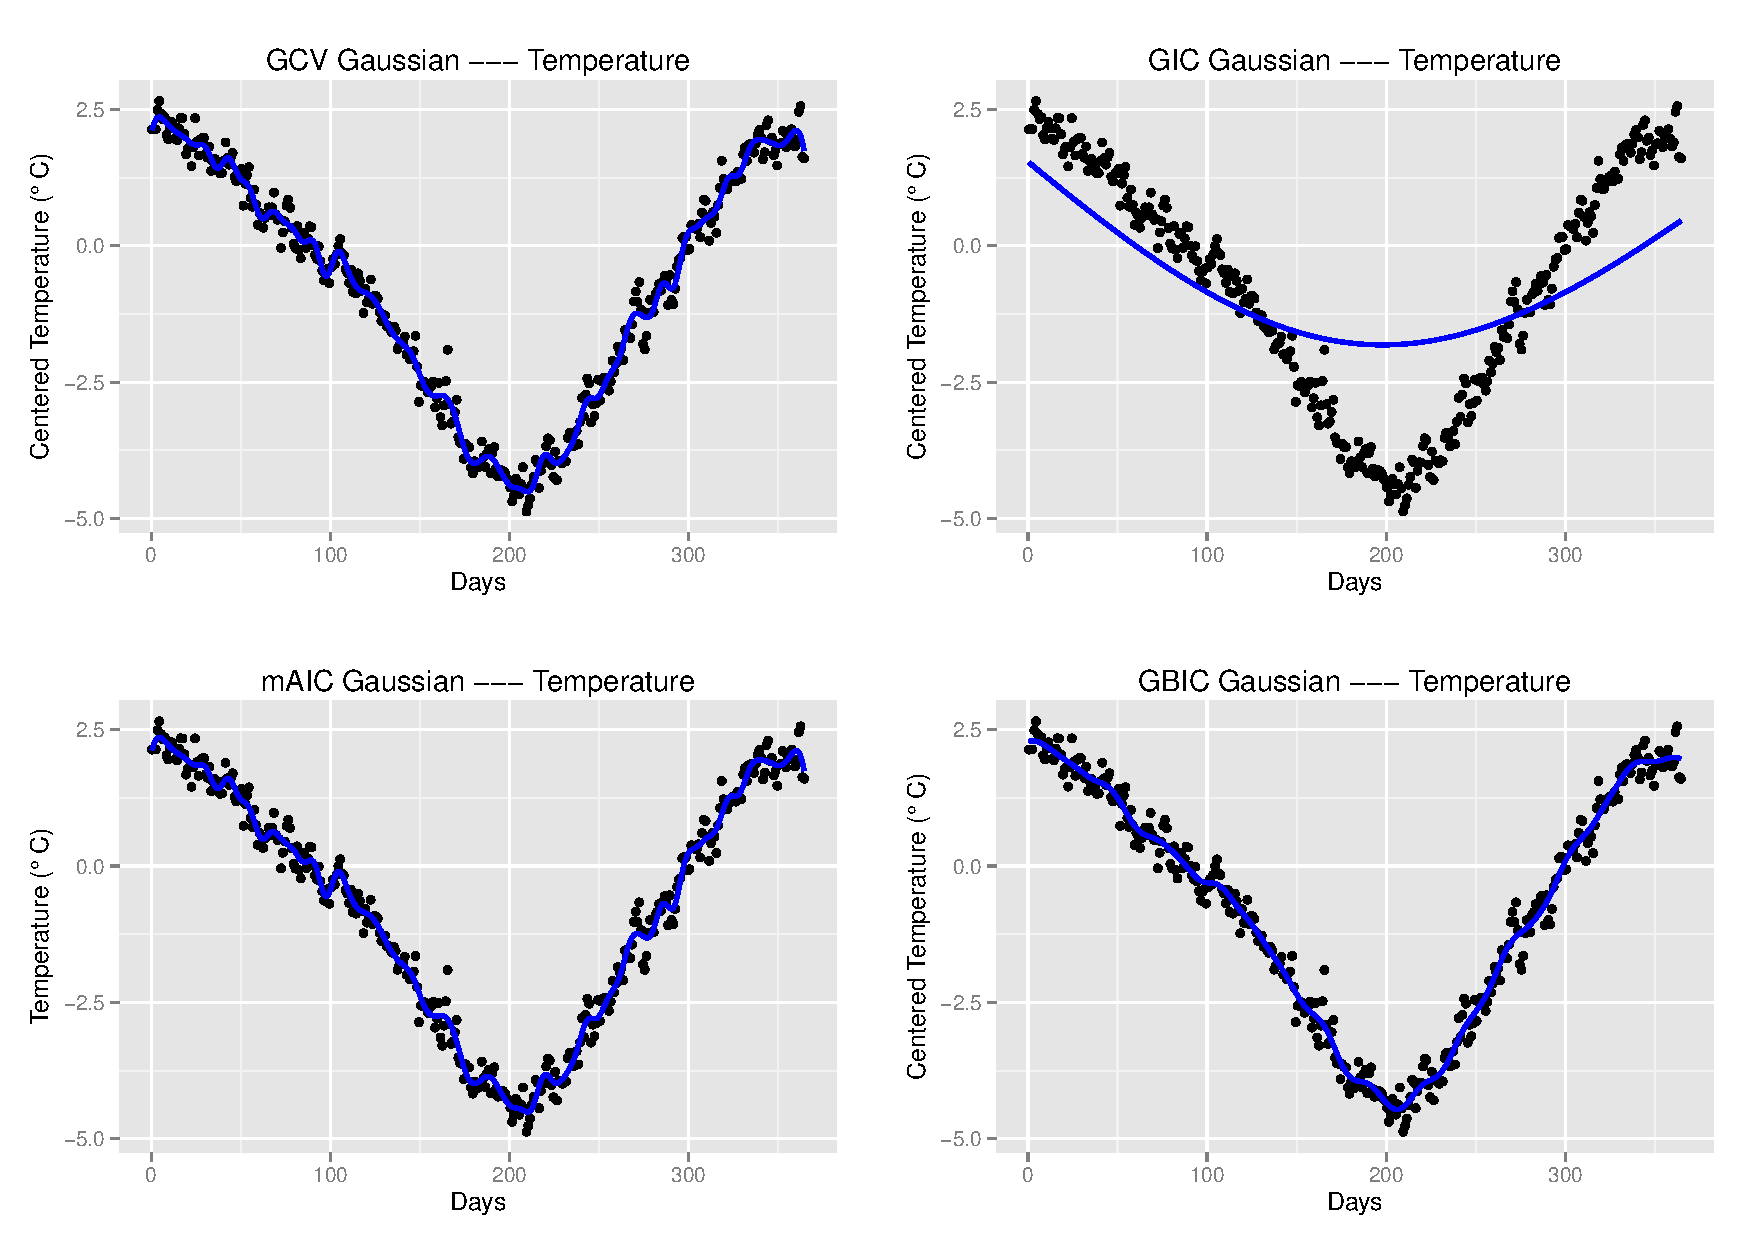
\includegraphics[height=12cm, width=1\textwidth]{Figures/Temp_Gauss_final.pdf}
  \caption[Fitting Temperature with \textit{Gaussian basis function} on \texttt{A CORUÑA} station]{\textbf{(a)} fitted curve using GCV; \textbf{(b)} fitted curve using GIC; \textbf{(c)} fitted curve using mAIC; \textbf{(d)} fitted curve using GBIC \\ on Temperatures in \texttt{A CORUÑA} }
  \label{fig:Temp_Gauss}
\end{figure}
\clearpage
\subsection{Wind Speed}
Figure~\ref{fig:wind_Gauss_2} depicts the fitted curves produced on the observed Wind Speed at \texttt{A CORUÑA} using the information from Table~\ref{table:table_all_stations}. For this specific scenario, the \textit{Generalized Information Criterion} results in $\hat{K} = 5$ and $\hat{\lambda} = 10^{-1.72}$, same as Temperature. The top right corner of Figure~\ref{fig:wind_Gauss_2} shows a very smooth curve (blue line) on top the raw data, which is a different story for the other model criteria.

\begin{figure}[th]
  %\centering
    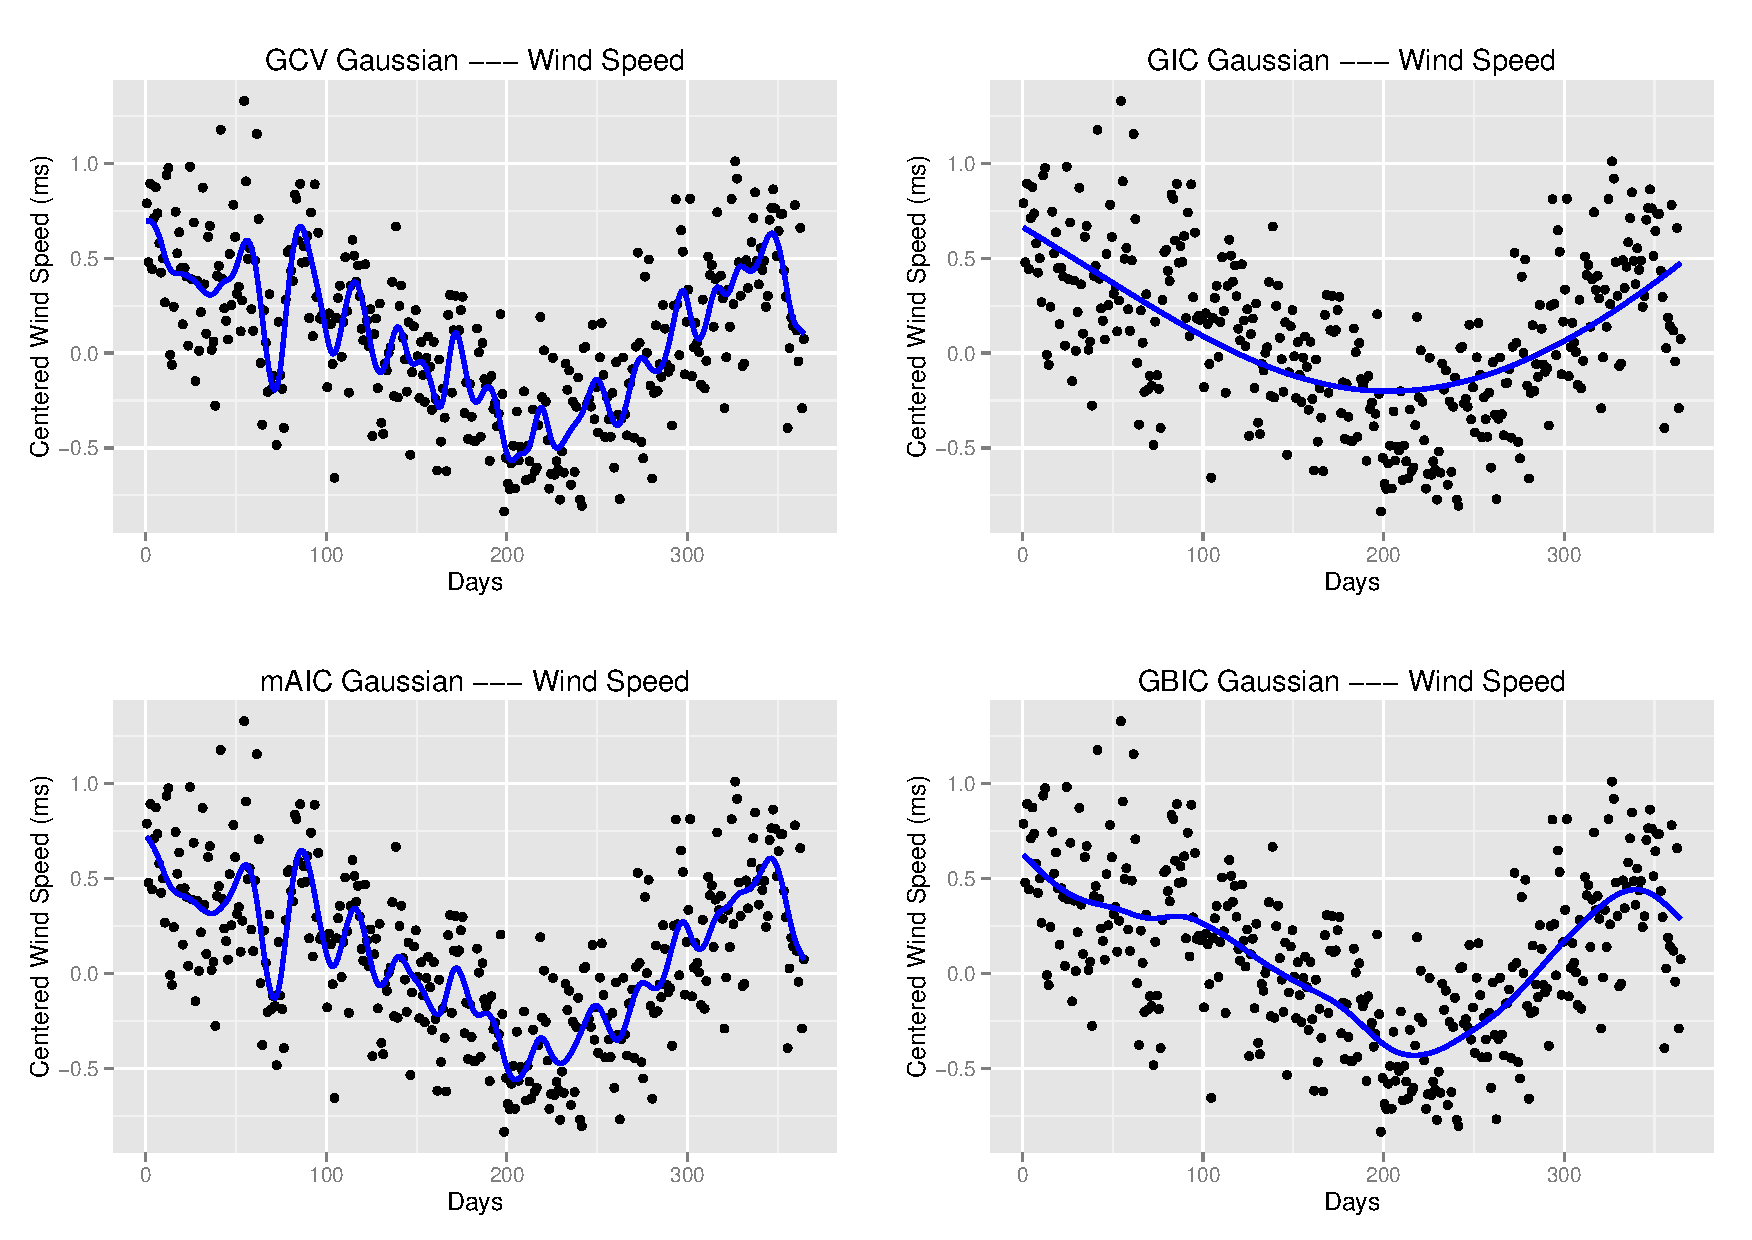
\includegraphics[height=12cm, width=1\textwidth]{Figures/Wind_Gauss_final.pdf}
  \caption[Fitting Wind Speed with \textit{Gaussian basis function} on \texttt{A CORUÑA} station]{\textbf{(a)} fitted curve using GCV; \textbf{(b)} fitted curve using GIC; \textbf{(c)} fitted curve using mAIC; \textbf{(d)} fitted curve using GBIC \\ on Wind Speed in \texttt{A CORUÑA}}
  \label{fig:wind_Gauss_2}
\end{figure}
\clearpage
\subsection{Log-Precipitation}
Computing the Log-Precipitation is done in two stages:\textbf{(1)} compute $\bm{D}$ then \textbf{(2)} compute $\bm{\hat{D}}$. Recall from Chapter~\ref{Chapter4} that $\bm{D}$ is a $N \times K_y$ matrix of coefficients with $N = 73$ and $K_y$ is the optimal number of basis functions computed following \textbf{Steps 1-4} from section~\ref{methodoly}. Their corresponding smoothing parameters $\hat{\lambda}$ are computed as well. The results are listed in Table~\ref{table:table_all_stations} of the Log-Precipitation using \textit{Gaussian Basis} functions. With all that information, it is possible to compute the matrices $\hat{\bm{\Sigma}}$ and $\hat{\bm{\mathcal{B}}}$ which yields to $\bm{\hat{D}}$. Because of hardware limitations, it is assumed that $\bm{\hat{D}}$ and $\bm{D}$ are of the same size and the optimization is only done on the smoothing parameters in order to get the optimal $\bm
{\Lambda}$. The use of equation~\eqref{hat_flrm} helps in calculating $\bm{\hat{D}}$.\\
Table~\ref{table:summary2} shows the optimal values $\text{log}_{10} (\hat{\lambda}_1)$ and $\text{log}_{10} (\hat{\lambda}_2)$ evaluated for all stations using each model criterion for a fixed the number of basis functions.
\begin{table}[ht]
\caption[Summary of the model selection on the Log-Precipitation using \textit{Gaussian basis functions}]{Summary of the model selection on the Log-Precipitation using \textit{Gaussian basis functions}}
\centering % used for centering table
\begin{tabular}{c @{\hspace{0.2cm}\vrule width 2pt\hspace{0.2cm}} c c c c } % centered columns (4 columns)
\hline %inserts double horizontal lines
\multicolumn{1}{c}{} & & & & \\[-2ex]
 \multicolumn{1}{c}{}& GCV & GIC & mAIC & GBIC \\ [0.5ex] % inserts table
%heading
\noalign{\hrule height 1pt} 
$\text{log}_{10} (\hat{\lambda}_1)$ & -3.41 & -1.42	& -3.72 & -2.33	\\
$\text{log}_{10} (\hat{\lambda}_2)$ & -2.1 & -1.92	& -2.1	& 0.33 \\
$\hat{K}$ & 51 & 5 & 48 & 63 \\
[0.25ex] % [1ex] adds vertical space
\hline  %inserts single line
\end{tabular}
\label{table:summary2} % is used to refer this table in the text
\end{table}

Figure~\ref{fig:logprec_Gauss} depicts the fitted curves produced on the observed Log-Precipitation at \texttt{A CORUÑA} using the information from Table~\ref{table:summary2}. The blue line represents the smooth curve computed using $\bm{D}$ and the red line represents the smooth curve derived from $\bm{\hat{D}}$. It can noted that the red lines has similar shape as the blue lines for each model criterion. Although the predicted curve for $\bm{\hat{D}}_{GIC}$ exhibits similar trend as the ones for $\bm{D}_{GIC}$, the fit is too smooth to be considered for further analysis. The top right corner plot confirms that statement. 

\newpage
\begin{landscape}
\thispagestyle{empty}
\begin{figure}[p]
  \centering
    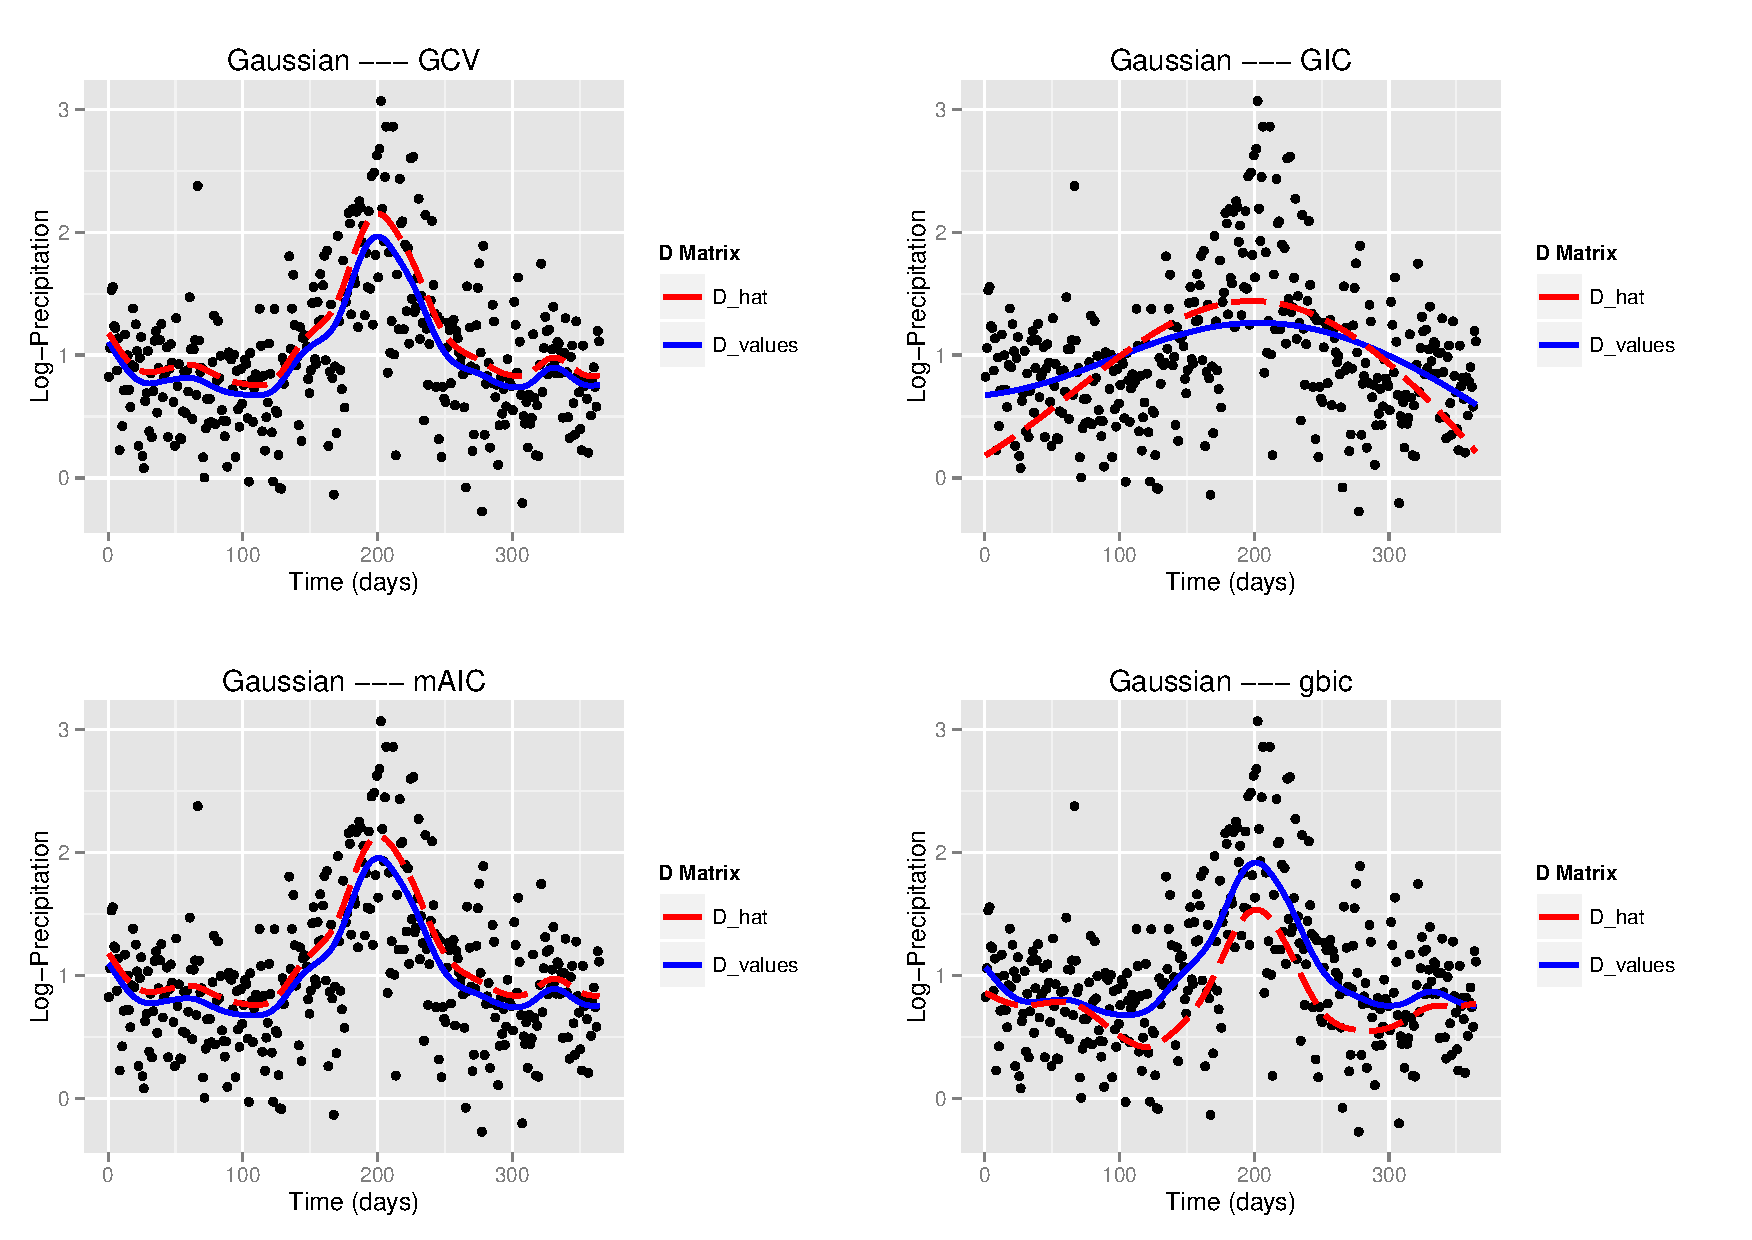
\includegraphics[height=15cm, width=1.7\textwidth]{Figures/D_hat_Gauss.pdf}
  \caption[Fitting Wind Speed with \textit{Gaussian basis function} on \texttt{A CORUÑA} station]{\textbf{(a)} fitted curve using GCV; \textbf{(b)} fitted curve using GIC; \textbf{(c)} fitted curve using mAIC; \textbf{(d)} fitted curve using GBIC \\ on Log-Precipitation in \texttt{A CORUÑA}}
  \label{fig:logprec_Gauss}
\end{figure}
\end{landscape}   
\newpage
%----------------------------------------------------------------------------------------
%	SECTION 2
%----------------------------------------------------------------------------------------

\section{Fourier Basis Functions}

The focus of this section is to model functional variables (independent variables and response variable) specified in equation~\eqref{chap5_eq1} using \textit{Fourier Basis} functions with \textit{Penalized Maximum Likelihood} estimate to compute the optimal model parameters $\hat{\bm{\Sigma}}$ amd $\hat{\bm{\mathcal{B}}}$.

\subsection{Temperature}
Figure~\ref{fig:Temp_fourier} depicts the fitted curves produced on the observed Temperature at \texttt{A CORUÑA} using the information from Table~\ref{table:table_all_stations}. For this case, once again the \textit{Generalized Information Criterion} has elected small values for $K$ and $\lambda$, smaller than the other model criteria. Clearly the small number of basis functions, has an important impact on the shape of the curve.

\begin{figure}[th]
  %\centering
    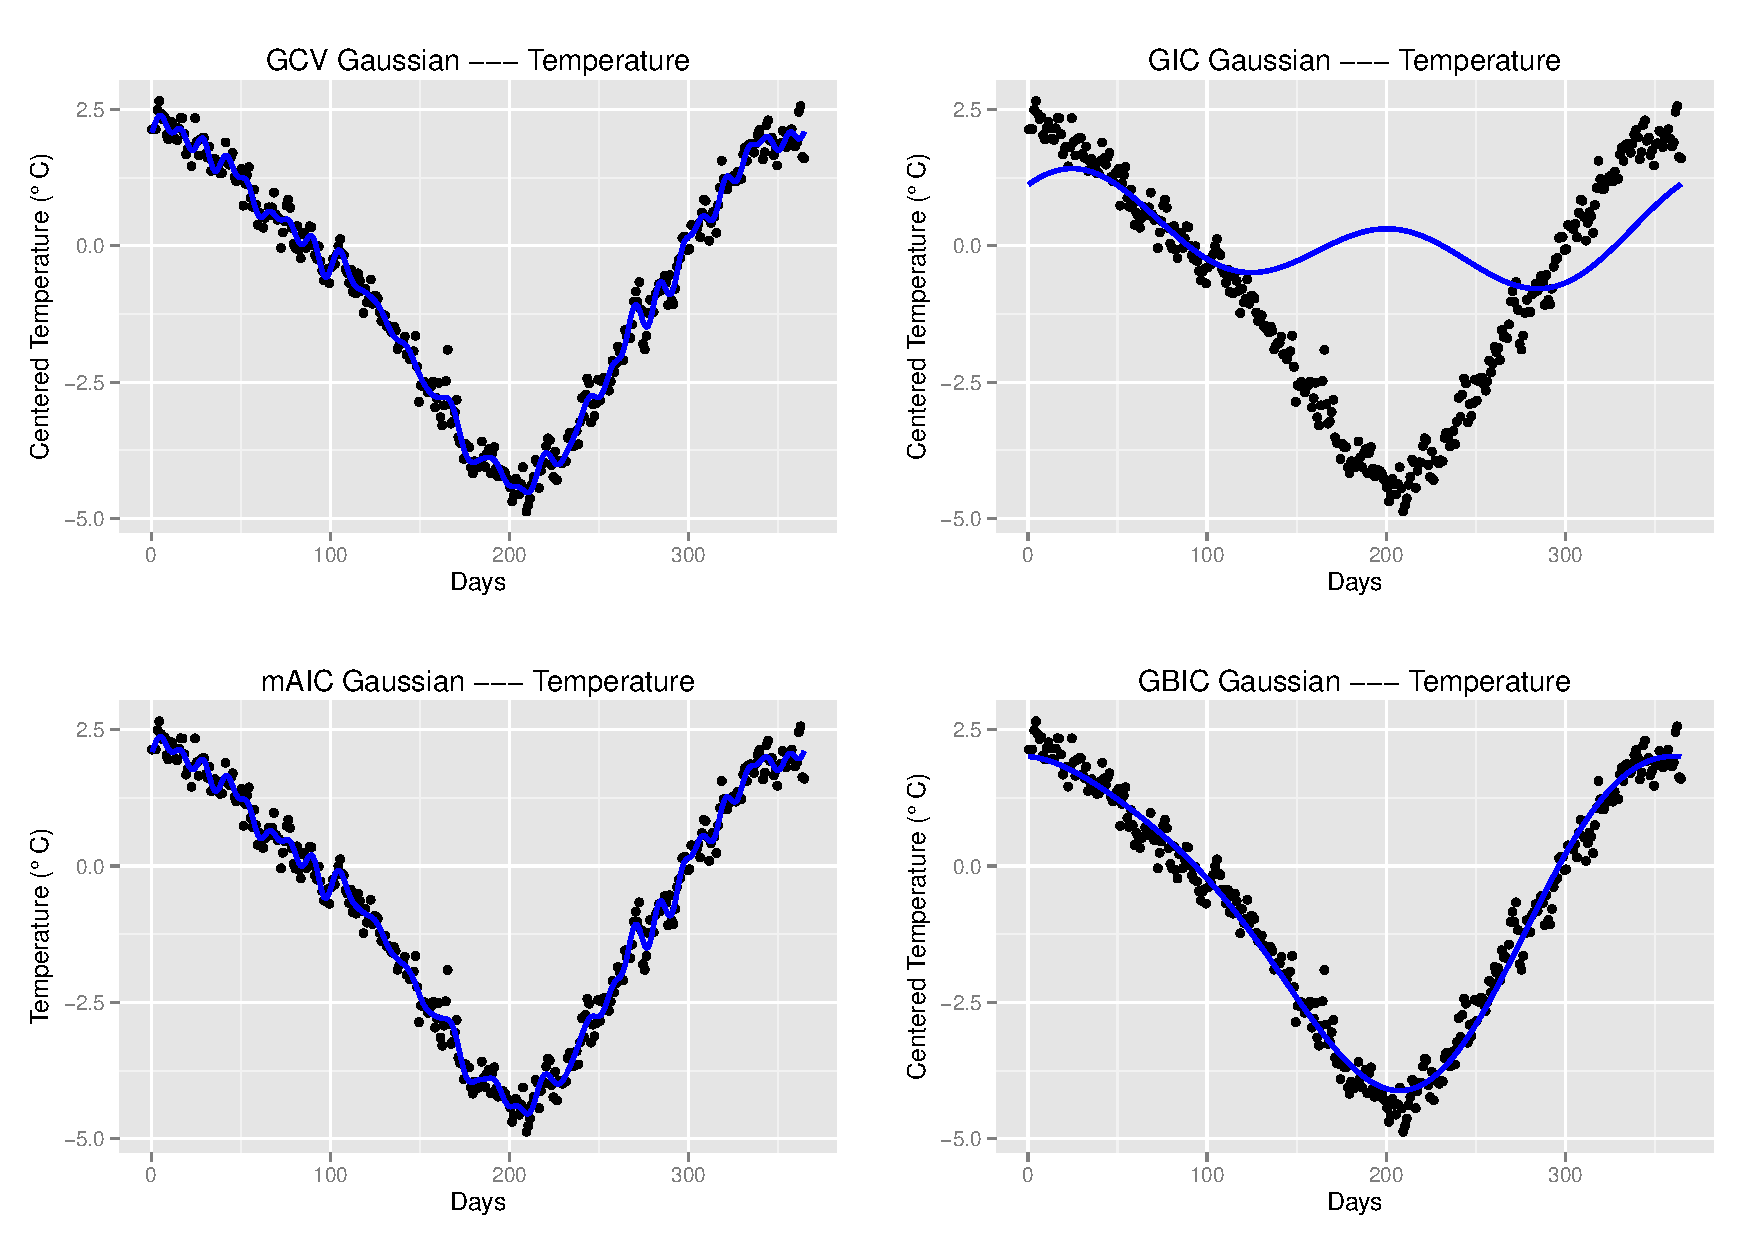
\includegraphics[height=12cm, width=1\textwidth]{Figures/Temp_fourier_plot.pdf}
  \caption[Fitting Temperature with \textit{Fourier basis function} on \texttt{A CORUÑA} station]{\textbf{(a)} fitted curve using GCV; \textbf{(b)} fitted curve using GIC; \textbf{(c)} fitted curve using mAIC; \textbf{(d)} fitted curve using GBIC \\ on Temperatures in \texttt{A CORUÑA} }
  \label{fig:Temp_fourier}
\end{figure}
\clearpage
\subsection{Wind Speed}
Figure~\ref{fig:Wind_fourier_plot} depicts the fitted curves produced on the observed Wind Speed at \texttt{A CORUÑA} using the information from Table~\ref{table:table_all_stations}. For this case, the \textit{Generalized Information Criterion} and the \textit{Generalized Bayesian Information Criterion} result in small $\hat{K}$ and small $\hat{\lambda}$. The top and bottow right hand side of Figure~\ref{fig:Wind_fourier_plot} show very smooth curves (blue line).
\begin{figure}[th]
  %\centering
    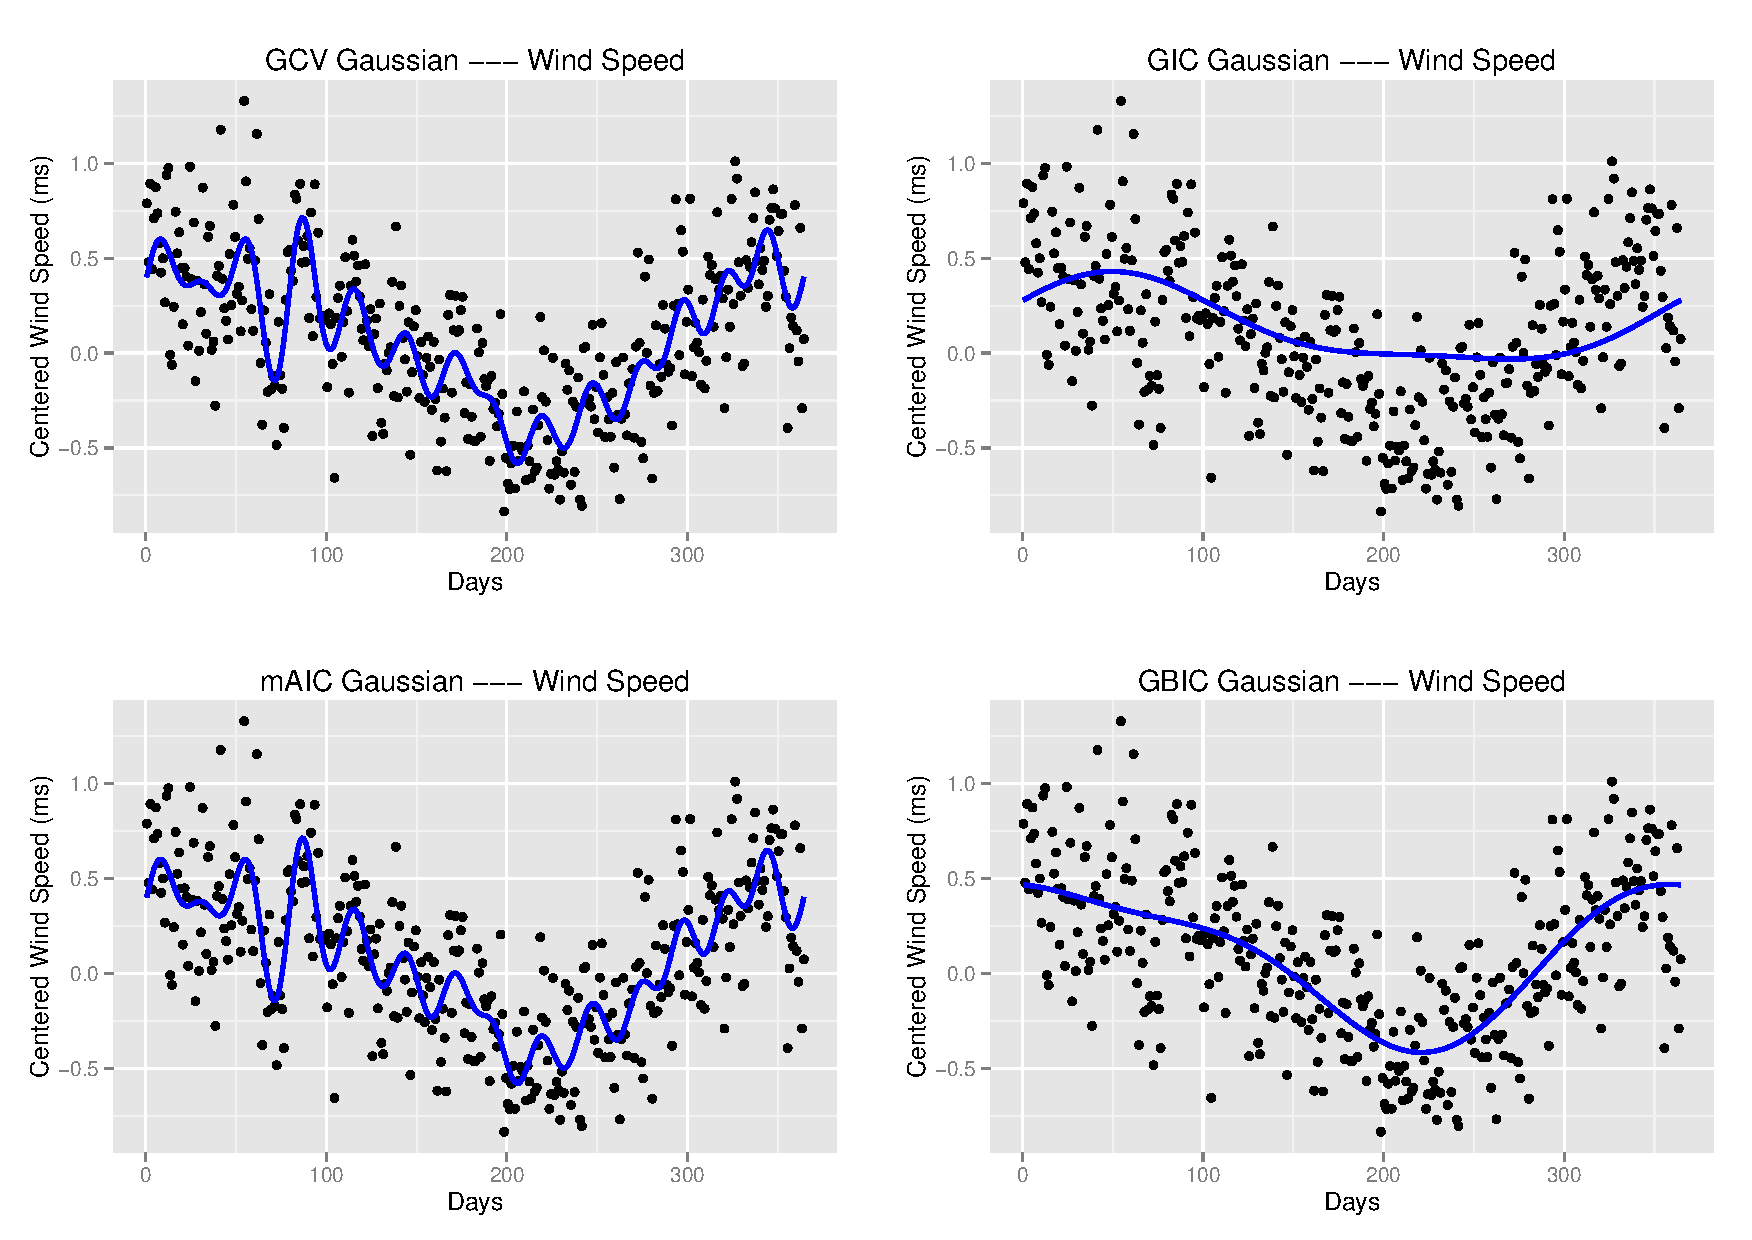
\includegraphics[height=12cm, width=1\textwidth]{Figures/Wind_fourier_plot.pdf}
  \caption[Fitting Wind Speed with \textit{Fourier basis function} on \texttt{A CORUÑA} station]{\textbf{(a)} fitted curve using GCV; \textbf{(b)} fitted curve using GIC; \textbf{(c)} fitted curve using mAIC; \textbf{(d)} fitted curve using GBIC \\ on Wind Speed in \texttt{A CORUÑA}}
  \label{fig:Wind_fourier_plot}
\end{figure}
\clearpage
\subsection{Log-Precipitation}
Table~\ref{table:summary4} shows the optimal values $\text{log}_{10} (\hat{\lambda}_1)$ and $\text{log}_{10} (\hat{\lambda}_2)$ evaluated for all stations using each model criterion for a fixed the number of basis functions. Note that the optimal number of basis functions is quite small for all basis functions and $\text{log}_{10} (\hat{\lambda})$ values are all negatives.
\begin{table}[ht]
\caption[Summary of the model selection on the Log-Precipitation using \textit{Fourier basis functions}]{Summary of the model selection on the Log-Precipitation using \textit{Fourier basis functions}}
\centering % used for centering table
\begin{tabular}{c @{\hspace{0.2cm}\vrule width 2pt\hspace{0.2cm}} c c c c } % centered columns (4 columns)
\hline %inserts double horizontal lines
\multicolumn{1}{c}{} & & & & \\[-2ex]
 \multicolumn{1}{c}{}& GCV & GIC & mAIC & GBIC \\ [0.5ex] % inserts table
%heading
\noalign{\hrule height 1pt} 
$\text{log}_{10} (\hat{\lambda}_1)$ & -4.83 & -1.52	& -5.25 & -5.17	\\
$\text{log}_{10} (\hat{\lambda}_2)$ & -3.92 & -1.25	& -4.21	& -5.17 \\
$\hat{K}$ & 7 & 7 & 7 & 5 \\
[0.25ex] % [1ex] adds vertical space
\hline  %inserts single line
\end{tabular}
\label{table:summary3} % is used to refer this table in the text
\end{table}

Figure~\ref{fig:logprec_fourier} depicts the fitted curves produced on the observed Log-Precipitation at \texttt{A CORUÑA} using the information from Table~\ref{table:summary3}. The blue line represents the smooth curve computed using $\bm{D}$ and the red line represents the smooth curve derived from $\bm{\hat{D}}$.

\newpage
\begin{landscape}
\thispagestyle{empty}
\begin{figure}[p]
  \centering
    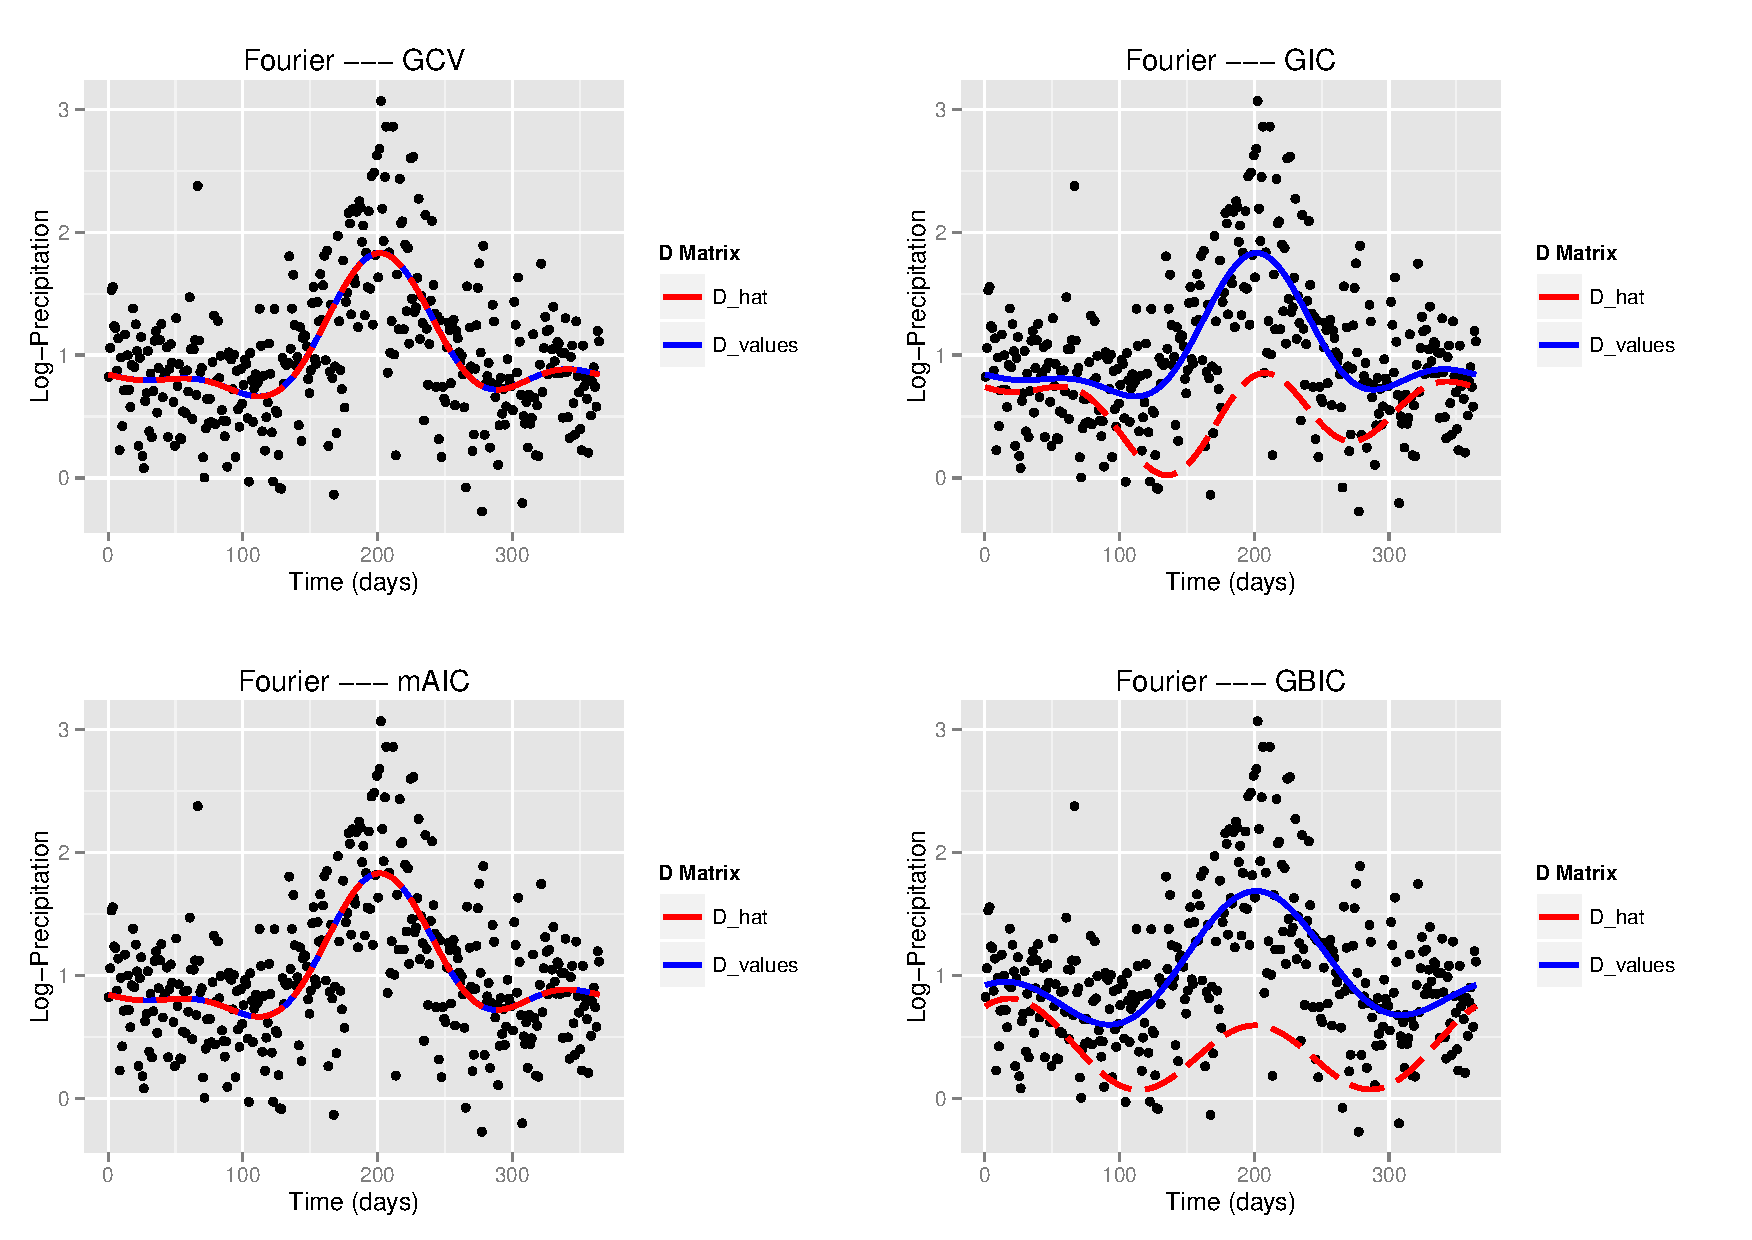
\includegraphics[height=15cm, width=1.7\textwidth]{Figures/D_hat_Fourier.pdf}
  \caption[Fitting Wind Speed with \textit{B-Splines basis function} on \texttt{A CORUÑA} station]{\textbf{(a)} fitted curve using GCV; \textbf{(b)} fitted curve using GIC; \textbf{(c)} fitted curve using mAIC; \textbf{(d)} fitted curve using GBIC \\ on Log-Precipitation in \texttt{A CORUÑA}}
  \label{fig:logprec_fourier}
\end{figure}
\end{landscape}   
\newpage

\section{B-Splines Basis Functions}
In this section the modeling is done using \textit{B-Splines basis functions} with \textit{Penalized Maximum Likelihood} estimate to calculate the functional the linear regression model (see equation~\eqref{chap5_eq1}). 

\subsection{Temperature}
Figure~\ref{fig:Temp_bsplines} shows the fitted curves produced on the observed Temperature at \texttt{A CORUÑA} using the information from Table~\ref{table:table_all_stations}. For this case, once again the \textit{Generalized Information Criterion} has elected small values for $K$ and $\lambda$, smaller than the other model criteria. Clearly the small number of basis functions, has an important impact on the shape of the curve.


\begin{figure}[th]
  %\centering
    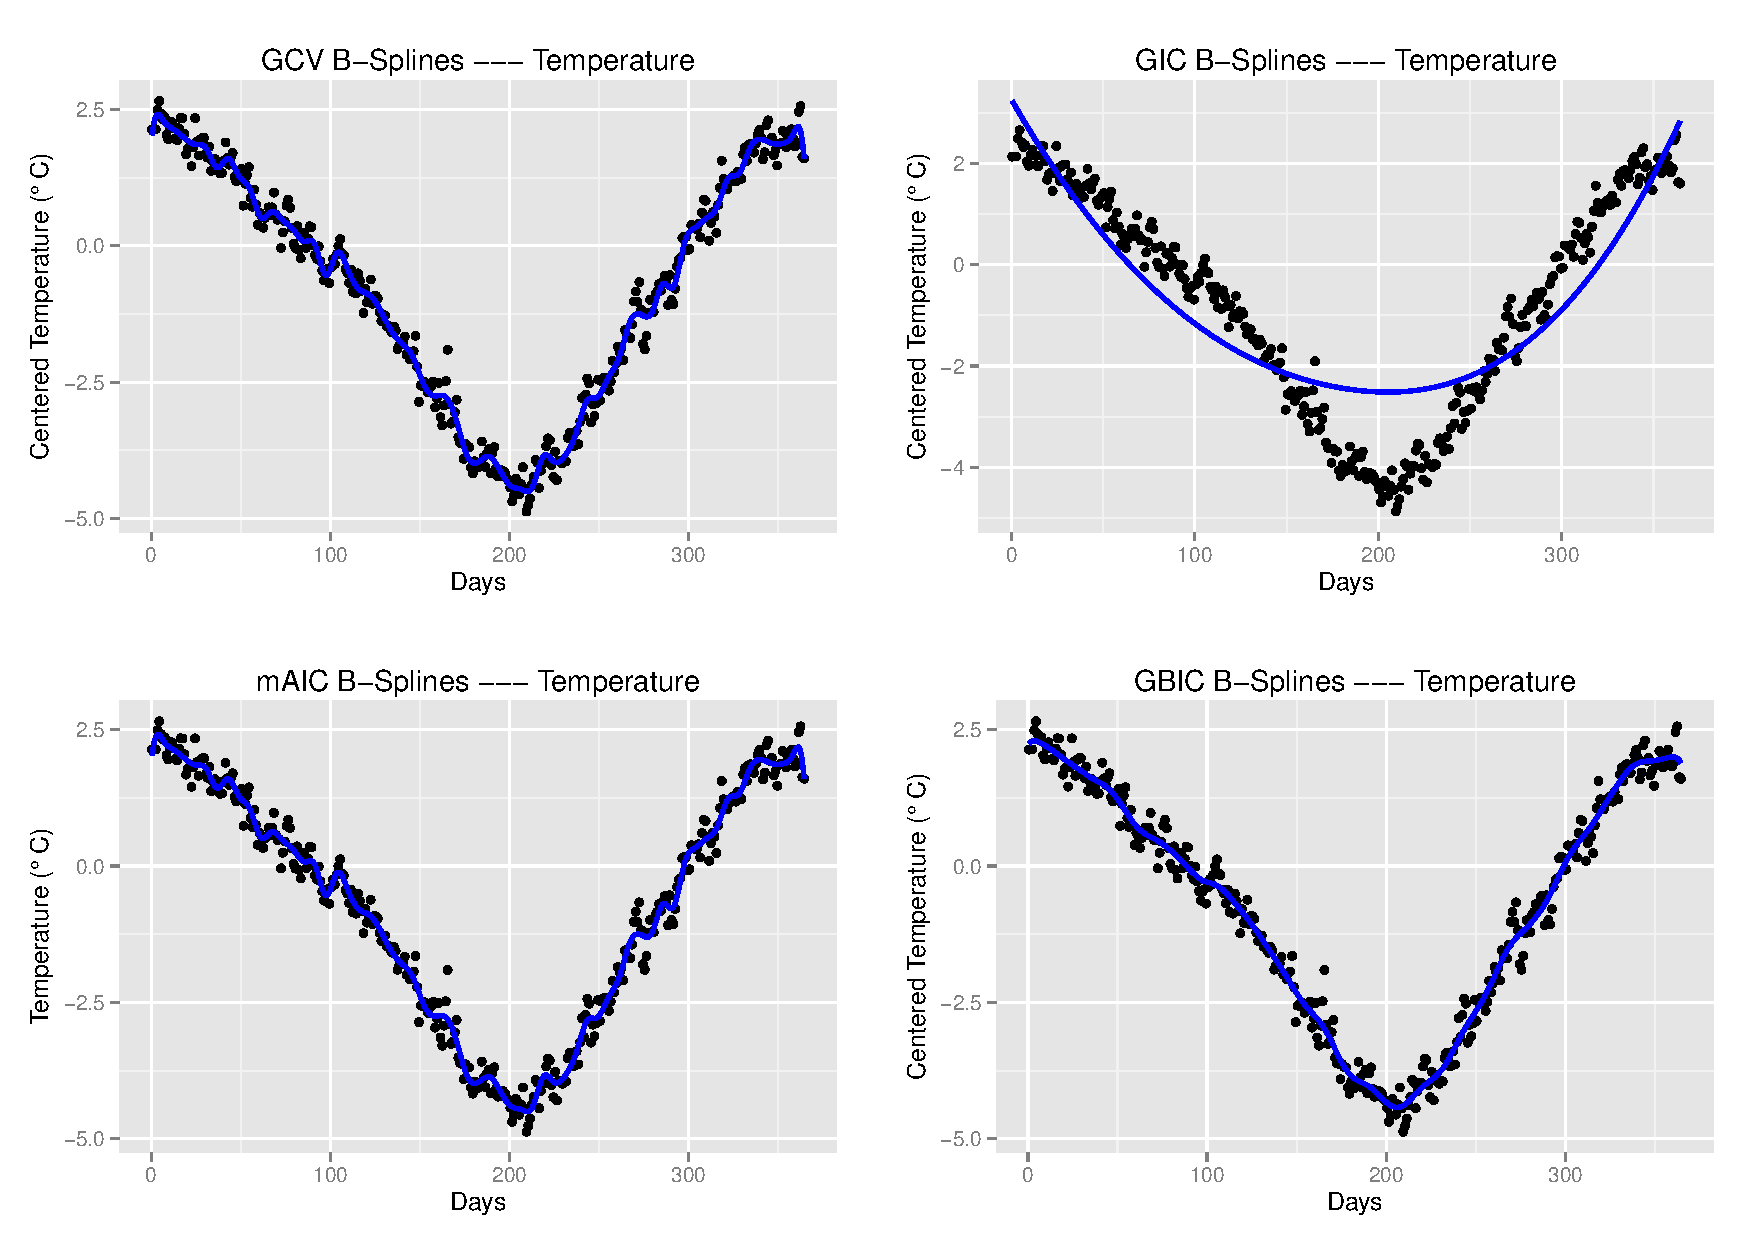
\includegraphics[height=12cm, width=1\textwidth]{Figures/Temp_bsplines_plot.pdf}
  \caption[Fitting Temperature with \textit{Gaussian basis function} on \texttt{A CORUÑA} station]{\textbf{(a)} fitted curve using GCV; \textbf{(b)} fitted curve using GIC; \textbf{(c)} fitted curve using mAIC; \textbf{(d)} fitted curve using GBIC \\ on Temperatures in \texttt{A CORUÑA} }
  \label{fig:Temp_bsplines}
\end{figure}
\clearpage
\subsection{Wind Speed}
Figure~\ref{fig:Wind_bsplines_plot} depicts the fitted curves produced on the observed Wind Speed at \texttt{A CORUÑA} using the information from Table~\ref{table:table_all_stations}. For this case, the \textit{Generalized Information Criterion} and the \textit{Generalized Bayesian Information Criterion} result in small $\hat{K}$ and small $\hat{\lambda}$. The top and bottow right hand side of Figure~\ref{fig:Wind_fourier_plot} show very smooth curves (blue line).

\begin{figure}[th]
  %\centering
    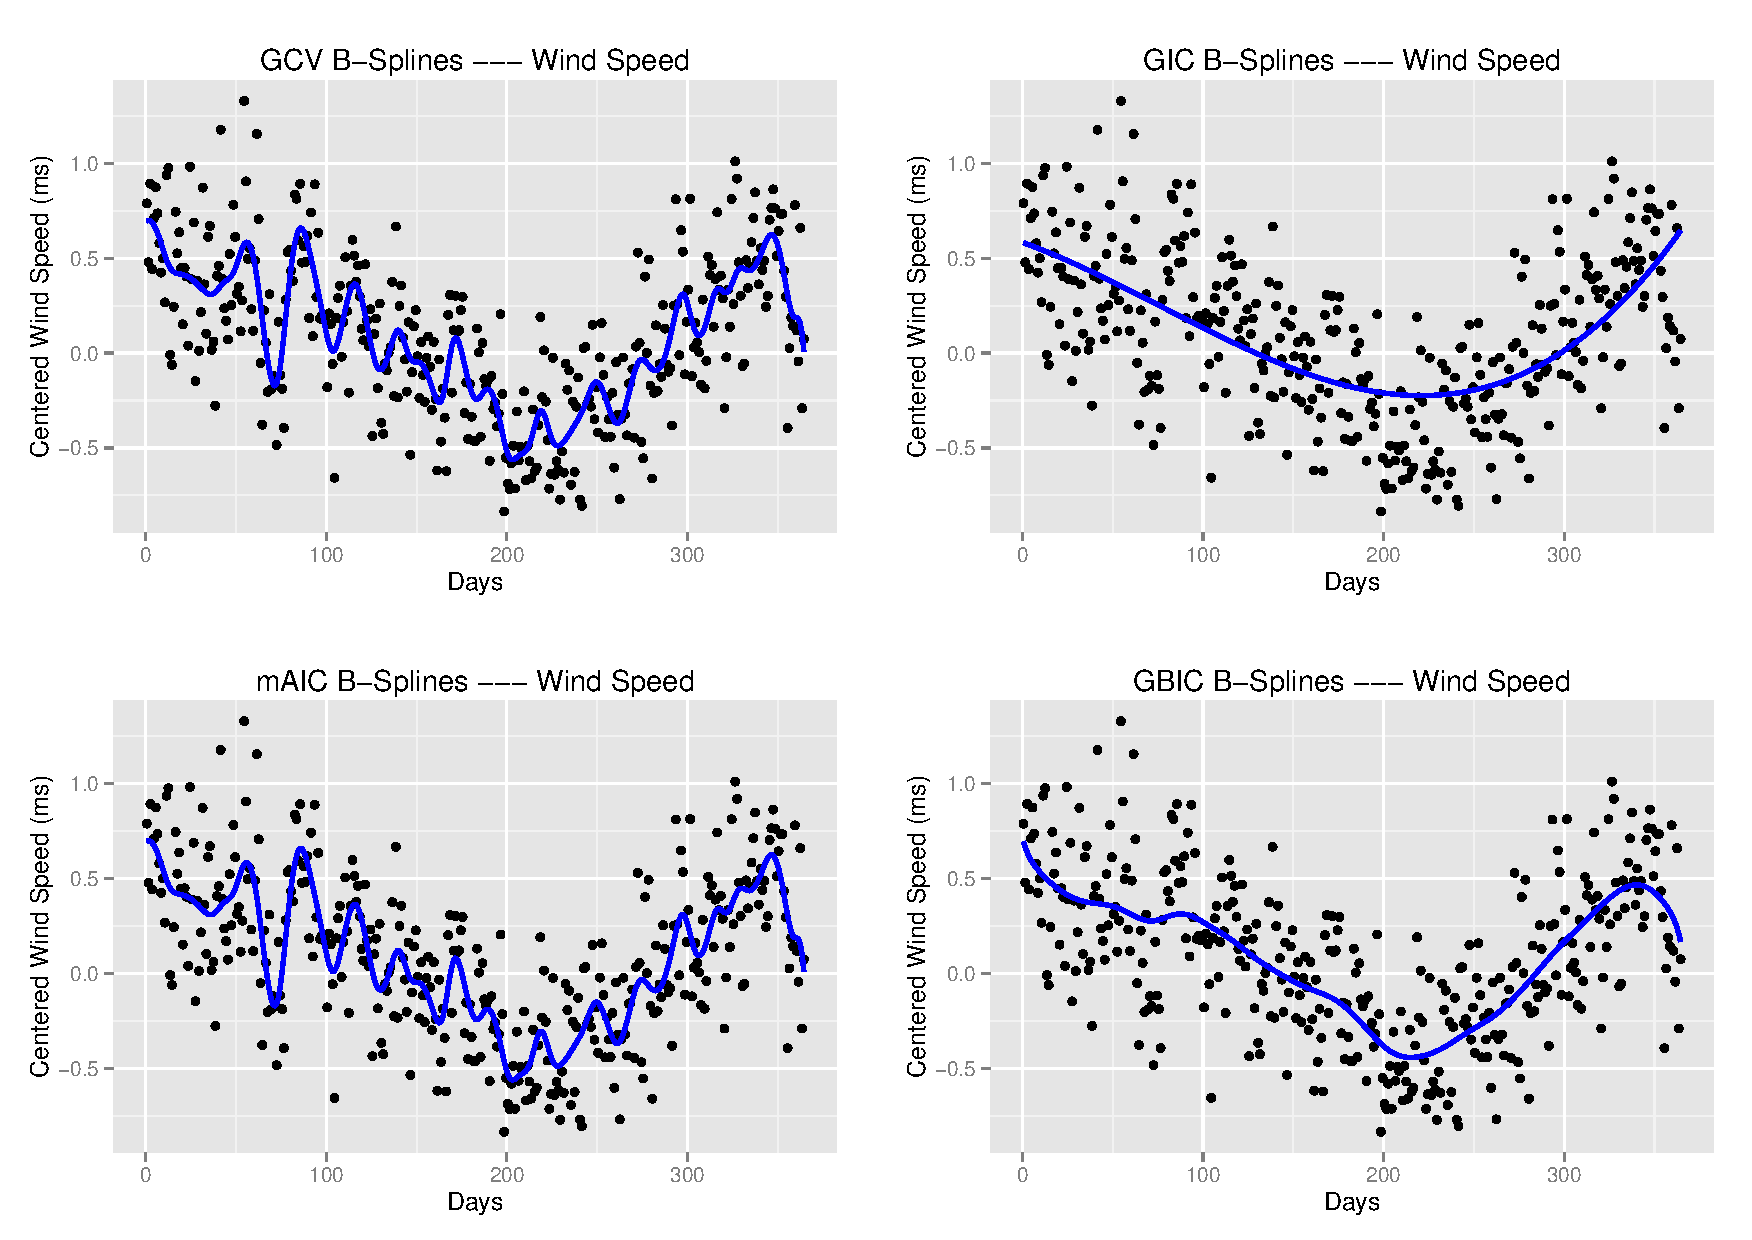
\includegraphics[height=12cm, width=1\textwidth]{Figures/Wind_bsplines_plot.pdf}
  \caption[Fitting Wind Speed with \textit{B-Splines basis function} on \texttt{A CORUÑA} station]{\textbf{(a)} fitted curve using GCV; \textbf{(b)} fitted curve using GIC; \textbf{(c)} fitted curve using mAIC; \textbf{(d)} fitted curve using GBIC \\ on Wind Speed in \texttt{A CORUÑA}}
  \label{fig:Wind_bsplines_plot}
\end{figure}
\subsection{Log-Precipitation}
The computation $\mathbf{\hat{D}}$ and consequently the predicted functional \textit{Log-Precipitation} implies optimizing the matrix of smoothing parameters $\bm{\Lambda}$ for fixed values of $K$ given in Table~\ref{table:table_all_stations}.
\\
Table~\ref{table:summary4} shows the optimal values $\text{log}_{10} (\hat{\lambda}_1)$ and $\text{log}_{10} (\hat{\lambda}_2)$ evaluated for all stations using each model criterion for a fixed the number of basis functions.
\begin{table}[ht]
\caption[Summary of the model selection on the Log-Precipitation using \textit{B-Splines basis functions}]{Summary of the model selection on the Log-Precipitation using \textit{B-Splines basis functions}}
\centering % used for centering table
\begin{tabular}{c @{\hspace{0.2cm}\vrule width 2pt\hspace{0.2cm}} c c c c } % centered columns (4 columns)
\hline %inserts double horizontal lines
\multicolumn{1}{c}{} & & & & \\[-2ex]
 \multicolumn{1}{c}{}& GCV & GIC & mAIC & GBIC \\ [0.5ex] % inserts table
%heading
\noalign{\hrule height 1pt} 
$\text{log}_{10} (\hat{\lambda}_1)$ & -3.51 & -2.15	& -3.72 & -1.33	\\
$\text{log}_{10} (\hat{\lambda}_2)$ & -1.98 & -1.42	& -2.1	& 1.23 \\
$\hat{K}$ & 65 & 5 & 65 & 63 \\
[0.25ex] % [1ex] adds vertical space
\hline  %inserts single line
\end{tabular}
\label{table:summary4} % is used to refer this table in the text
\end{table}

Figure~\ref{fig:logprec_bsplines} depicts the fitted curves produced on the observed Log-Precipitation at \texttt{A CORUÑA} using the information from Table~\ref{table:summary4}. The blue line represents the smooth curve computed using $\bm{D}$ and the red line represents the smooth curve derived from $\bm{\hat{D}}$.

\newpage
\begin{landscape}
\thispagestyle{empty}
\begin{figure}[p]
  \centering
    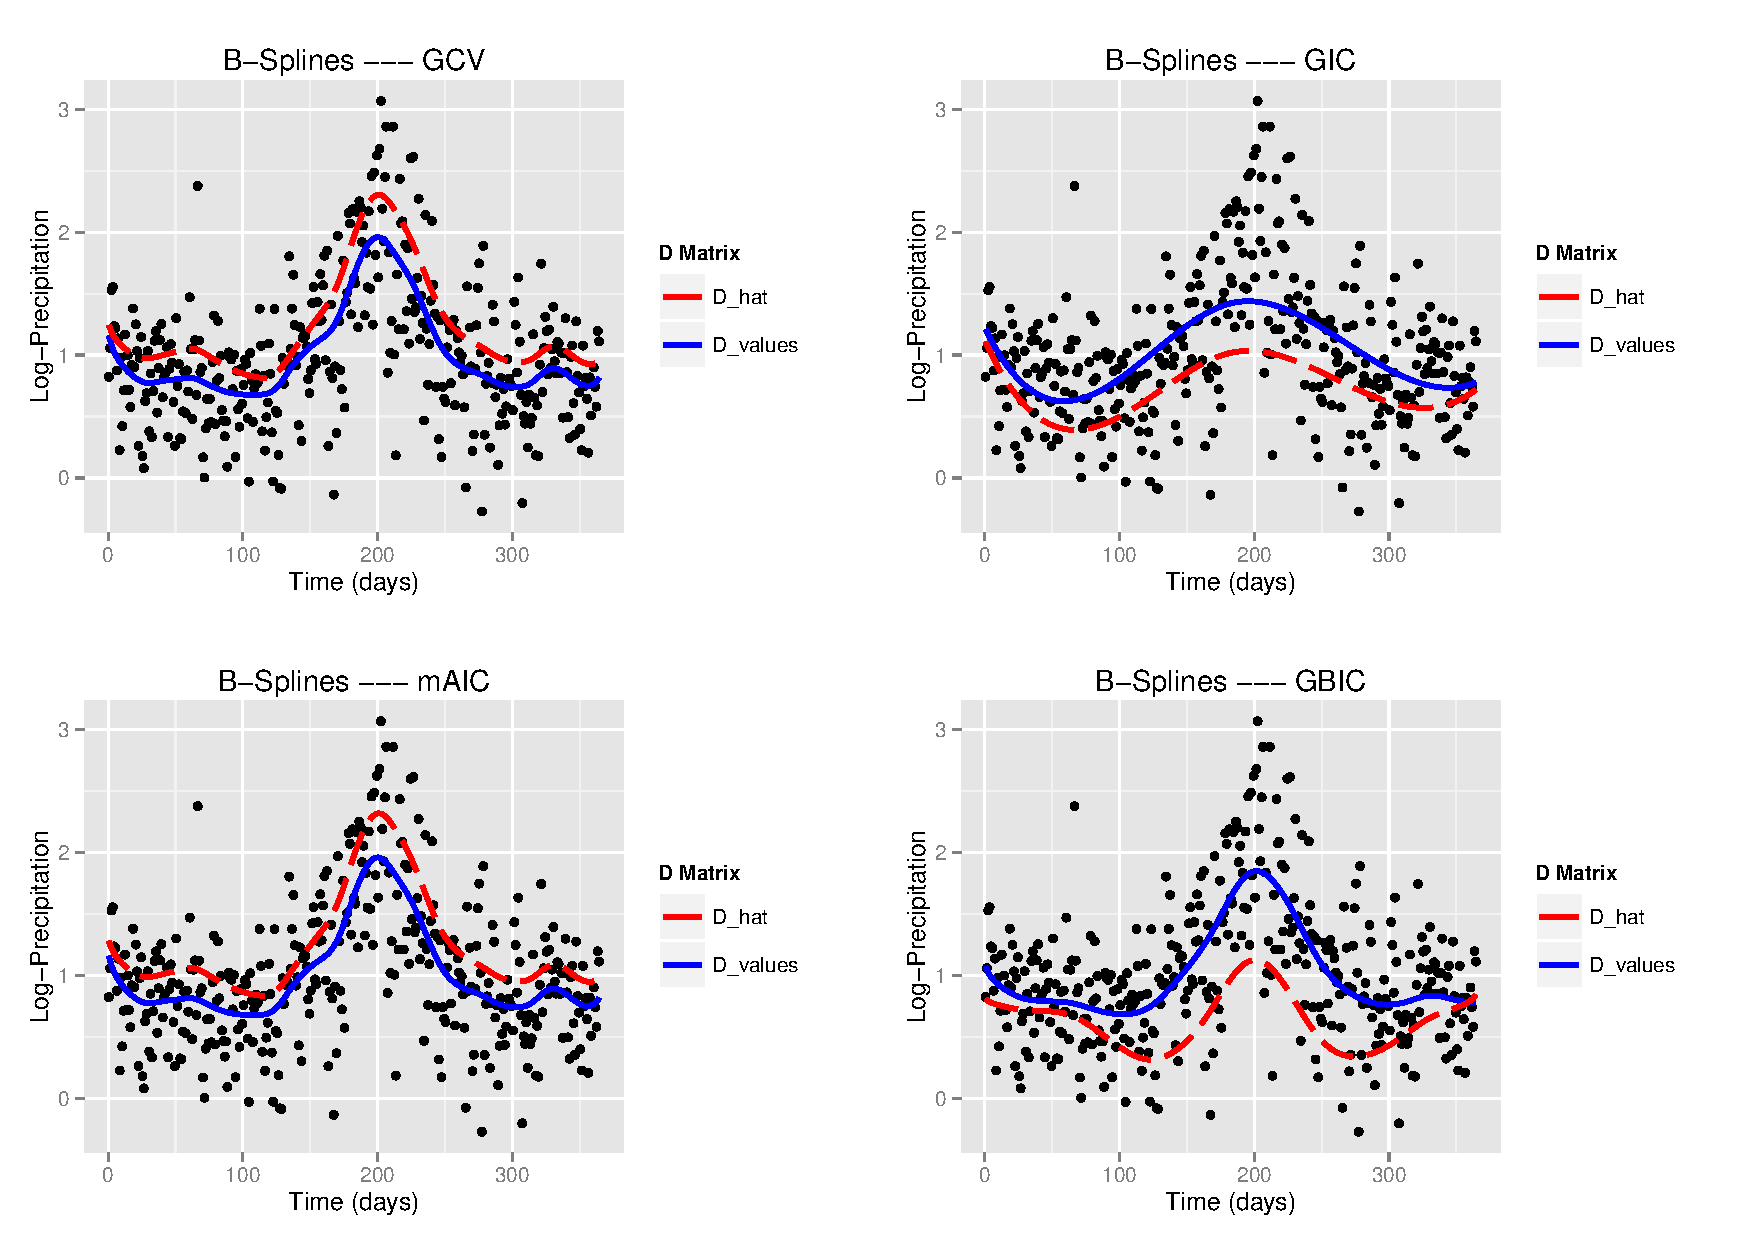
\includegraphics[height=15cm, width=1.7\textwidth]{Figures/D_hat_Bsplines.pdf}
  \caption[Fitting Wind Speed with \textit{Gaussian basis function} on \texttt{A CORUÑA} station]{\textbf{(a)} fitted curve using GCV; \textbf{(b)} fitted curve using GIC; \textbf{(c)} fitted curve using mAIC; \textbf{(d)} fitted curve using GBIC \\ on Log-Precipitation in \texttt{A CORUÑA}}
  \label{fig:logprec_bsplines}
\end{figure}
\end{landscape}   
\newpage

\section{Discussion of the Results}
The objective of this chapter was to illustrate the implementation of a Functional Linear Regression model~\eqref{chap5_eq1} when both covariates and the response variable are functional. The dataset used for illustration was the Spanish weather data. The aim was to model the functional behaviour of the Log-Precipitation when the functional behaviour of the Temperature and Wind Speed were known. The Functional Linear regression Model was computed using the \textit{Penalized Maximum Likelihood} estimate and four model criteria were used to evaluate the model namely: the \textit{Generalized Cross-Validation}; the \textit{Generalized Information Criteria}; the \textit{modified Akaike Information Criteria} and the \textit{Generalized Bayesian Information Criteria}. Three kinds of basis functions were used in the analysis: \textit{Gaussian Basis} function; \textit{Fourier Basis} function and \textit{B-Splines Basis} function. For each kind of basis function and each model criterion, the optimal number of basis functions $\hat{K}$ was estimated as well as the optimal smoothing parameter $\hat{\lambda}$. It was found that, each variable modeled using each kind of basis functions evaluated using each kind model criterion resulted in more or less different values for $\hat{K}$ and the smoothing parameter.
\\
Table~\ref{table:amse} shows the \textit{Mean Square Error} averaged across all stations, for each model criterion and for each type of basis function. In this context, the \textit{Mean Square Error} is defined as the difference between the actual observed data and the predicted: $\bm{\hat{D}} \bm{\Phi}(t)$. Comparing these values across each model criteria is not a very objective way to reach a meaningful conclusion. In fact, it is sensible to compare the results across all types of basis functions.
As given on Table~\ref{table:amse}, the lowest \textit{Average Mean Square Error} (AMSE), considering all models criteria, is found to be at \textit{Gaussian Basis} function. The next type of basis functions is \textit{B-Splines Basis} followed by \textit{Fourier Basis} which appeared to perform the worst out of all three.

\begin{table}[ht]
\caption[\textit{Average Mean Square Error} for the predicted versus observed values of the the functional  \textit{Log-Precipitation}]{\textit{Average Mean Square Error} for the predicted versus observed values of the functional Log-Precipitation} % title of Table
\centering % used for centering table
\begin{tabular}{c c c c} % centered columns (4 columns)
\hline\hline %inserts double horizontal lines
Model Criterion & \textit{Gaussian Basis} & \textit{B-Splines Basis} & \textit{Fourier Basis} \\ [0.5ex] % inserts table
%heading
\hline % inserts single horizontal line
GCV & 0.759 & 0.808 & 0.772 \\ % inserting body of the table
GIC & 1.680 & 1.750 & 2.6 \\
mAIC & 0.759 & 0.791 & 0.772 \\
GBIC & 1.24 & 1.403 & 1.674 \\ [1ex] % [1ex] adds vertical space
\hline %inserts single line
\end{tabular}
\label{table:amse} % is used to refer this table in the text
\end{table}
 
% Chapter Template

\chapter{Conclusion} % Main chapter title

\label{Chapter6} % Change X to a consecutive number; for referencing this chapter elsewhere, use \ref{Chapter6}

\lhead{Chapter 6. \emph{Conclusion}} % Change X to a consecutive number; this is for the header on each page - perhaps a shortened title

%----------------------------------------------------------------------------------------
%	SECTION 1
%----------------------------------------------------------------------------------------


This Chapter will summarize the results of the research and its applications  subject to the dissertation. The Chapter will begin with a discussion of the objectives mentioned in Chapter~\ref{Chapter1} in a concluding manner. An overview and a brief summary of the illustrations implemented in Chapter~\ref{Chapter5} are done. Some comments will be made on the hardware specifications used to run the scripts as well as their limitations in performing the analysis. Finally, some recommendations will be made to those interested in future research regarding Functional Linear Regression Modeling.


%-----------------------------------
%	SUBSECTION 1
%-----------------------------------
\section{Concluding Remarks about Objectives}
Below each of the objectives stated in Chapter~\ref{Chapter1} is discussed.
\begin{itemize}
\item The first objective stated in Chapter~\ref{Chapter1} was to define Functional Data Analysis and introduce important basis functions that were used throughout the dissertation. Chapter~\ref{Chapter2} offered an in-depth explanation of the different basis expansions used in FDA and provided a visualization aspect to them. The emphasis was on the revelant techniques and methods in this dissertation, namely: \textit{Gaussian}, \textit{Fourier} and \textit{B-Splines}.
\item Chapter~\ref{Chapter2} provided an in-depth understanding of four different model criteria (i.e. \textit{Generalized Cross-Validation}, \textit{Generalized Information Criterion}, \textit{modified Akaike Information Criterion} and \textit{Generalized Bayesian Information Criterion}) as well their computations in \texttt{R} through examples, in the FDA context. Chapter~\ref{Chapter4} and Chapter~\ref{Chapter5} provided the insight of the aforementioned model criteria in the FLRM context. Appendix~\ref{AppendixA} was fully dedicated in the implementation of the most recurrent steps done when converting discrete observed data to a functional process. 
\item Chapter~\ref{Chapter3} main objective was to provide the mathematical foundations to have a better understanding of the link between Functional Analysis and Functional Data Analysis. Key definitions and theorems were given in order to equip the readers with the relevant background to understand the meaning of the \textit{Kahrunen-Loeve} Theorem.
\item In Chapter~\ref{Chapter4}, the Functional Linear Regression was introduced. All the different model estimation methods with a deeper attention on the \textit{Penalized Maximum Likelihood} estimate. The derivations of the maximum likelihood estimators, in every case, were computed. The model criteria in the FLRM context were defined and derived accordingly, see Appendix~\ref{AppendixB} for the proofs.
\item Chapter~\ref{Chapter5} provided an application of FLRM using the \texttt{Aemet} data. The \textit{Gaussian Basis}, \textit{Fourier Basis} and \textit{B-Splines Basis} were used to smooth the discretized observed data of Temperature, Wind Speed and Log-Precipitation for all 73 stations. For each basis, the four model criteria were used to compute the optimal model parameters. Once the functional data of Log-Precipitation were obtained, the Functional Linear Regression was implemented to predict the functional data of Log-Precipitation (see Figures \ref{fig:logprec_Gauss}, \ref{fig:logprec_fourier} and \ref{fig:logprec_bsplines}). The AMSE was computed to compare the different basis functions. Based on the results, it appeared that the \textit{Gaussian Basis} outperformed all the other basis functions.
\end{itemize}

%-----------------------------------
%	SUBSECTION 2
%-----------------------------------

\section{Limitations}
One of the major issues with performing an analysis in Functional Linear Regression Modeling is the time taken to compute the functional variables. It is clear that when the number of data points $J$ is very large, computing an expansion in $\mathcal{O}(J)$ operations is critical. Additionally, when the operations are performed over a number of sets of observed data (e.g. weather stations) then the computation takes even more time to be completed. Another computationally intensive process is the implementation of model criteria. \textit{Generalized Cross-Validation}, for instance, is known to be computationally intensive and therefore requires a lot of space in memory. This is a particular issue when running codes using the Programming Language \texttt{R}. A typical error message displayed when trying to compute matrix operations would be: \texttt{Error: cannot allocate vector of size 78.1 Gb}.\\
For this dissertation, the only focus was on Regression in Functional Data Analysis. The functional behaviour of the Log-Precipitation was predicted assuming the functional behaviours of Temperature and Wind Speed were known. This particularity of the \texttt{Aemet} data and of weather data in general is difficult to find. In other words, the availability of datasets that have similar features as the weather data is not given. Even when the dataset is available, the discretized observed points are sparse which makes the analysis in functional context strenuous.


%----------------------------------------------------------------------------------------
%	SECTION 2
%----------------------------------------------------------------------------------------

\section{Recommendations}
As already mentioned, the analysis of Functional Linear Regression was done using the \texttt{Aemet} weather data only. More datasets with similar intrisic features as the weather data from other fields of research should be investigated to involve more scientists in Functional Data Analysis. The \texttt{R}-package \texttt{fda} by \cite{Ramsay2009FDA} has been around for a long time and is the most popular package for FDA. Unfortunately, the package is a bit restricted with other kinds of analysis involving: other types of basis functions (e.g. \textit{Gaussian Basis}); other types of model evaluations methods (e.g. \textit{Penalized Maxmum Likelihood} method) and other types model criteria (e.g. GIC, mAIC, GBIC). More packages must be released in that regard.\\
When it comes to Functional Linear Regression models, one of the main assumption is that the chosen basis function is the one that smooth the predictor and covariates. Which is not always a correct assumption because different variables exhibit different stochastic paths. One of the challenges with violating that assumption is the computation of the matrices $\bm{J}_{\phi \psi}$ where $\bm{\phi}(t)$ could be a \textit{Fourier Basis} function and $\bm{\psi}(t)$\textit{Gaussian Basis} function.\\
Thus there is still vast unexplored area of research in the field of Functional Data Analysis in general and specifically for Functional Regression Modeling. This dissertation provides a first step in that direction. 
%\input{Chapters/Chapter7} 

%----------------------------------------------------------------------------------------
%	THESIS CONTENT - APPENDICES
%----------------------------------------------------------------------------------------

\addtocontents{toc}{\vspace{2em}} % Add a gap in the Contents, for aesthetics

\appendix % Cue to tell LaTeX that the following 'chapters' are Appendices

% Include the appendices of the thesis as separate files from the Appendices folder
% Uncomment the lines as you write the Appendices

% Appendix A

\chapter{\texttt{R}-Functions} % Main appendix title

\label{AppendixA} % For referencing this appendix elsewhere, use \ref{AppendixA}

\lhead{Appendix A. \emph{\texttt{R}-Functions}} % This is for the header on each page - perhaps a shortened title

In order to make some of the \texttt{R}-codes readable, most of the repeated operations have been wrapped up into functions that are used throughout the dissertation.
\section{Matrices of Basis Functions and Model Selection}
  \\
  \\[1ex]
  \mbox{
    \begin{tabular}{ c c c c}
    \hline \\[-0.75ex]
    \hspace{1cm} \texttt{Gaussian\_bsplines} &  \hspace{.5cm} \textit{Gaussian Basis} functions with \textit{B-Splines} & & \\
    \\[-0.75ex] 
    \hline\\[-5ex]
    \end{tabular}%
  }
\subsection*{Description}
This function is used to compute a matrix of \textit{Gaussian Basis} functions with \textit{B-Splines}. Its arguments are:
\begin{itemize}
\item \texttt{tt} being the vector of values $\left\lbrace t_{1},\dots,t_{J} \right\rbrace \in \mathcal{T}$;
\item \texttt{m} represents the number of basis functions applied to the function.
\end{itemize}

\subsection*{\texttt{R}-Code}
\begin{lstlisting}
  Gaussian_bsplines = function(tt,m){
    
    range <- diff(range(tt))
    kn <- seq(min(tt) - (range/(m-3))*3, max(tt) + (range/(m-3))*3, by = range/(m-3))
    myu <- kn[3:(m+2)]
    h <- diff(kn,lag = 2)/3
    
    B <- matrix(0,length(tt),(m))
    for (j in 1:m){
      B[,j] <- exp(-0.5*(tt-myu[j])^2/(h[1]^2))
    }
    return(B)
  }
 \end{lstlisting}
\vspace{0.5cm}
  \mbox{
    \begin{tabular}{ c c c c}
    \hline \\[-0.75ex]
    \hspace{.5cm} \texttt{Gaussian\_kmeans} &  \hspace{1cm} \textit{Gaussian Basis} functions with \texttt{K-Means} & & \\
    \\[-0.75ex] 
    \hline\\[-1ex]
    \end{tabular}%
  }
  \subsection*{Description}
  This function is used to compute a matrix of \textit{Gaussian Basis} functions using \textit{K-means}. Its arugments are:
 \begin{itemize}
 \item \texttt{tt} is used to specify the vector of values $\left\lbrace t_{1},\dots,t_{J} \right\rbrace \in \mathcal{T}$;
 \item \texttt{m} is used to specify the number of basis functions applied to the function;
 \item \texttt{nyu} is used to specify the hyperparameter.
 \end{itemize} The clustering method used is the one developed by \cite{Hartigan1979}. 
 \subsection*{\texttt{R}-Code}
 \begin{lstlisting}
  Gaussian_kmeans = function(tt,m,nyu){
     
    k <- kmeans(tt, centers = m,algorithm = "Hartigan-Wong")
    myu <- as.vector(k$centers)
    h <- k$withinss/k$size    
     
    B <- matrix(0,length(tt),(m))
    for (j in 1:m){
      B[,j] <- exp(-0.5*(tt-myu[j])^2/(h[j]*nyu))
    }
    return(B)
  }
  \end{lstlisting}
\clearpage
\\
 \\
 \\[3ex]
 \mbox{
   \begin{tabular}{ c c c c}
   \hline \\[-0.75ex]
   \hspace{1cm} \texttt{Bsplines\_FDA} &  \hspace{1cm} \textit{B-Splines Basis} functions & \hspace{1cm} & \hspace{1.5cm} \\
   \\[-0.75ex] 
   \hline\\[-4ex]
   \end{tabular}%
 }
\subsection*{Description}
This function is used to generate a matrix of \textit{B-Splines Basis} functions. It uses the \texttt{R}-package \texttt{fda}. Its arguments are:
\begin{itemize}
\item \texttt{tt} is used to specify the vector of values $\left\lbrace t_{1},\dots,t_{J} \right\rbrace \in \mathcal{T}$;
\item \texttt{m} is used to specify the number of basis functions applied to the function.
\item \texttt{norder} is used to specify the order of the \textit{B-Splines}
\end{itemize}
\subsection*{\texttt{R}-Code}
\begin{lstlisting}
Bsplines_FDA <- function(tt,m,norder=4){
  require(fda)
  basis = create.bspline.basis(rangeval = range(tt),nbasis = m,norder)
  B <- eval.basis(evalarg = tt,basisobj = basis)
  return(B)
} 
\end{lstlisting} 
\vspace{0.5cm}
 \mbox{
   \begin{tabular}{ c c c c}
   \hline \\[-0.75ex]
   \hspace{1cm} \texttt{Fourier\_FDA} &  \hspace{1cm} \textit{Fourier Basis} functions & \hspace{2cm} & \hspace{1.5cm} \\
   \\[-0.75ex] 
   \hline\\[-2ex]
   \end{tabular}%
 }
\subsection*{Description}
This function is used to generate a matrix of \textit{Fourier Basis} functions. It uses the \texttt{R}-package \texttt{fda}. Its arguments are:
\begin{itemize}
\item \texttt{tt} is used to specify the vector of values $\left\lbrace t_{1},\dots,t_{J} \right\rbrace \in \mathcal{T}$;
\item \texttt{m} is used to specify the number of basis functions applied to the function.
\end{itemize}
\clearpage
\subsection*{\texttt{R}-Code}
\begin{lstlisting}
Fourier_FDA <- function(tt,m){
  require(fda)
  if((m %% 2)==0) {m <- m + 1} else {m <- m}
  basis = create.fourier.basis(rangeval = range(tt),nbasis = m)
  B <- eval.basis(evalarg = tt,basisobj = basis)
  return(B)
}
\end{lstlisting}
\vspace{0.5cm}
\mbox{
   \begin{tabular}{ c c c c}
   \hline \\[-0.75ex]
   \hspace{.5cm} \texttt{\texttt{Pen\_Max\_Likelihood}} &  \hspace{1cm} \textit{Penalized Maximum Likelihood} estimate &\hspace{-0.5cm} & \\
   \\[-0.75ex] 
   \hline\\[-2ex]
   \end{tabular}%
}
\subsection*{Description}
This function is used to compute the \textit{Penalized Maximum Likelihood} estimate. Its arguments are:
\begin{itemize}
\item \texttt{B} is used to specify the matrix of basis functions;
\item \texttt{n} is used to specify the number of basis functions;
\item \texttt{lambda} is used to specify log${}_{10}(\lambda)$;
\item \texttt{y} is used for the vector of observed values.
\end{itemize}
\subsection*{\texttt{R}-Code}
\begin{lstlisting}
Pen_Max_Likelihood <- function(B, n, lambda, y){
  D <- matrix(0,(n-2),n)
  D[1, ] <- c(1,-2,1,rep(0,(n-3)))
  for (i in 1:(n-4)) {
    D[(i+1), ] <- c(rep(0,i),1,-2,1,rep(0,(n-3)-i))
  }
  D[(n-2), ] <- c(rep(0,(n-3)),1,-2,1)
  K <- t(D)%*%D
  
  lamda <- 10^(lambda)
  sigma <- 2
  sigma1 <- 1
  
  while((sigma-sigma1)^2 > 1e-7){
    Binv <- solve(t(B)%*%B+ncol(train.temp)*(lamda)*(sigma)*K,diag(ncol(K)))
    w <- (Binv)%*%t(B)%*%y[1,]
    sigma1 <- sigma
    sigma1 <- as.vector(sigma1)
    sigma <- (1/ncol(train.temp))*t(y[1,]-B%*%w)%*%(y[1,]-B%*%w)
    sigma <- as.vector(sigma)       
  }
  list(lamda=lamda,sigma=sigma,K=K,w=w)
}
\end{lstlisting}

\section{Model Criterion}
\vspace{0.5cm}
 \mbox{
   \begin{tabular}{ c c c c}
   \hline \\[-0.75ex]
   \hspace{1cm} \texttt{gcv\_fun} &  \hspace{1cm} \textit{Generalized Cross-Validation} criterion& \hspace{2cm} & \hspace{1cm}\\
   \\[-0.75ex] 
   \hline\\[-1ex]
   \end{tabular}%
 }
\subsection*{Description}
This function is used to compute the \textit{Generalized Cross-Validation} criterion for model evaluation. Its arguments are:
\begin{itemize}
\item \texttt{ob} is used to specify the object created from the \texttt{Pen\_Max\_Likelihood} function;
\item \texttt{y} is used for the vector of observed values;
\item \texttt{tt} is used to specify the vector of values $\left\lbrace t_{1},\dots,t_{J} \right\rbrace \in \mathcal{T}$.
\end{itemize}

\subsection*{\texttt{R}-Code}
\begin{lstlisting}
gcv_fun <- function(tt, y, ob){
  Binv <- solve(t(B)%*%B+length(y)*(ob$lamda)*(ob$sigma)*ob$K,diag(n))
  H <- B%*%(Binv)%*%t(B)
  yhat <- H%*%y[1,]
  den = 1 - sum(diag(H))/length(tt) # load(matrixcalc)
  y.diff = yhat - y[1,]
  return(mean((y.diff/den)^2))
}
\end{lstlisting}
\vspace{0.5cm}
 \mbox{
   \begin{tabular}{ c c c c}
   \hline \\[-0.75ex]
   \hspace{1cm} \texttt{gic\_fun} &  \hspace{1cm} \textit{Generalized Information Criterion} & \hspace{2.5cm} & \\
   \\[-0.75ex] 
   \hline\\[-1ex]
   \end{tabular}%
 }
\subsection*{Description} 
This function is used to compute the \textit{Generalized Information Criterion} for model evaluation. Its arguments are:
\begin{itemize}
\item \texttt{ob} is used to specify the object created from the \texttt{Pen\_Max\_Likelihood} function;
\item \texttt{y} is used for the vector of observed values;
\item \texttt{tt} is used to specify the vector of values $\left\lbrace t_{1},\dots,t_{J} \right\rbrace \in \mathcal{T}$.
\end{itemize}
\subsection*{\texttt{R}-Code}
\begin{lstlisting}
gic_fun <- function(y,ob,n){
  gamma <- diag(as.vector(y[1,]-B%*%ob$w))
  one <- rep(1,length(y))
  
  R1 <- rbind(t(B)%*%B+length(y)*(ob$lamda)*(ob$sigma)*ob$K,t(one)%*%gamma%*%B/(ob$sigma))
  R2 <- rbind(t(B)%*%gamma%*%one/(ob$sigma),length(y)/(2*(ob$sigma)))
  R <- cbind(R1,R2)
  R <- R/(length(y)*(ob$sigma))
  if(det(R) < 10^(103)) {Rinv <- solve(R,diag(n+1))} else {Rinv <- NA}
  
  Q1 <- rbind(t(B)%*%(gamma)^2%*%B/(ob$sigma)-(ob$lamda)*ob$K%*%ob$w%*%t(one)%*%gamma%*%B,t(one)%*%(gamma)^3%*%B/(2*(ob$sigma)^2)-t(one)%*%gamma%*%B/(2*(ob$sigma)))
  Q2 <- rbind(t(B)%*%(gamma)^3%*%one/(2*(ob$sigma)^2)-t(B)%*%gamma%*%one/(2*(ob$sigma)),t(one)%*%(gamma)^4%*%one/(4*(ob$sigma)^3)-length(y)/(4*(ob$sigma)))
  Q <- cbind(Q1,Q2)
  Q <- Q/(length(y)*(ob$sigma))
  
  V <- ifelse(det(R) < 10^(103) & all(!is.na(Rinv)), length(y)*(log(2*pi)+1)+length(y)*log(ob$sigma)+2*sum(diag(Rinv%*%Q)), NA)
  return(V)
}
\end{lstlisting}
\vspace{0.5cm}
 \mbox{
   \begin{tabular}{ c c c c}
   \hline \\[-0.75ex]
   \hspace{1cm} \texttt{mAIC\_fun} &  \hspace{1cm} \textit{modified Akaike Information Criterion} & \hspace{1.5cm} & \\
   \\[-0.75ex] 
   \hline\\[-1ex]
   \end{tabular}%
 }
\subsection*{Description} 
This function is used to compute the \textit{modified AIC} method for model evaluation. Its arguments are:
\begin{itemize}
\item \texttt{ob} is used to specify the object created from the \texttt{Pen\_Max\_Likelihood} function;
\item \texttt{y} is used for the vector of observed values;
\item \texttt{tt} is used to specify the vector of values $\left\lbrace t_{1},\dots,t_{J} \right\rbrace \in \mathcal{T}$.
\end{itemize}
\subsection*{\texttt{R}-Code}
\begin{lstlisting}
mAIC_fun <- function(ob,y,n){
  Binv <- solve(t(B)%*%B+length(y)*(ob$lamda)*(ob$sigma)*ob$K,diag(n))
  H <- B%*%(Binv)%*%t(B)
  return(length(y)*(log(2*pi)+1)+length(y)*log(ob$sigma)+2*sum(diag(H)))
}
\end{lstlisting}
\vspace{0.5cm}
 \mbox{
   \begin{tabular}{ c c c c}
   \hline \\[-0.75ex]
   \hspace{.5cm} \texttt{gbic\_fun} &  \hspace{1cm} \textit{Generalized Bayesian Information Criterion} &\hspace{1cm} & \\
   \\[-0.75ex] 
   \hline\\[-1ex]
   \end{tabular}%
 }
\subsection*{Description}
This function is used to compute the \textit{Generalized Bayesian Information Criterion} for model evaluation. Its arguments are:
\begin{itemize}
\item \texttt{ob} is used to specify the object created from the \texttt{Pen\_Max\_Likelihood} function;
\item \texttt{y} is used for the vector of observed values;
\item \texttt{tt} is used to specify the vector of values $\left\lbrace t_{1},\dots,t_{J} \right\rbrace \in \mathcal{T}$.
\end{itemize}
The \texttt{R}-code is as follows:
\begin{lstlisting}
gbic <- function(y,ob,n){
  gamma <- as.vector(y[1,]-B%*%ob$w)
  
  Q1 <- rbind(t(B)%*%B+length(y)*(ob$lamda)*(ob$sigma)*ob$K,t(gamma)%*%B/(ob$sigma))
  Q2 <- rbind(t(B)%*%gamma/(ob$sigma),length(y)/(2*(ob$sigma)))
  Q <- cbind(Q1,Q2)
  Q <- Q/(length(y)*(ob$sigma))
  Q.det <- det(Q)
  vec <- eigen(ob$K)$values
  vec <- vec[vec >= 0]
  
  return((length(y)+n-1)*log(ob$sigma) + length(y)*(ob$lamda)*(ob$sigma)*t(ob$w)%*%ob$K%*%ob$w/(ob$sigma) + length(y) + (length(y)-3)*log(2*pi)+
    3*log(length(y)) + log(Q.det) - log(prod(vec)) - (n-1)*log((ob$lamda)*(ob$sigma)))
}
\end{lstlisting}
\clearpage
 \mbox{
   \begin{tabular}{ c c c c}
   \hline \\[-0.75ex]
   \hspace{1cm} \texttt{GCV.Gauss\_bs} &  \hspace{1cm} \textit{Generalized Cross-Validation}$^2$ &\hspace{2cm} & \\
   \\[-0.75ex] 
   \hline\\[-4ex]
   \end{tabular}%
 }
\subsection*{Description}
  This function computes the \textit{Generalized Cross-Validation} criterion using the \textit{Least Squares} method without a smoothing parameter based Gaussian basis function with \textit{B-Splines}. Its arguments are:
  \begin{itemize}
  \item \texttt{dat} is used to specify the $N \times J$ matrix of observations;
  \item \texttt{tt} is used to specify the vector of values $\left\lbrace t_{1},\dots,t_{J} \right\rbrace \in \mathcal{T}$;
  \item \texttt{m} is used to specify the number of basis functions applied to the function.
  \end{itemize} 
  This function is used run for illustrative purpose (see section~\ref{foreach})
  \subsection*{\texttt{R}-Code}
  \begin{lstlisting}
   S = NULL
   GCV.Gauss_bs = function(dat,tt,m){
     
     range <- diff(range(tt))
     kn <- seq(min(tt) - (range/(m-3))*3, max(tt) + (range/(m-3))*3, by = range/(m-3))
     myu <- kn[3:(m+2)]
     h <- diff(kn,lag = 2)/3
      
     B <- matrix(0,length(tt),(m))
     for (j in 1:m){
       B[,j] <- exp(-0.5*(tt-myu[j])^2/(h[1]^2))
     }
     Binv <- solve(t(B)%*%B,diag(m))
     S <- B%*%Binv%*%t(B)
     xhat <- S%*%dat
     den <- 1 - sum(diag(S))/length(tt)
     x.diff <- xhat - dat
     return(mean((x.diff/den)^2)) # GCV value
  }
    \end{lstlisting}

% Appendix Template

\chapter{Derivations and Proofs} % Main appendix title

\label{AppendixB} % Change X to a consecutive letter; for referencing this appendix elsewhere, use \ref{AppendixX}

\lhead{Appendix B. \emph{Derivations and Proofs}} % Change X to a consecutive letter; this is for the header on each page - perhaps a shortened title

\section{Karhunen-Loeve proofs}

The coefficients in theorem~\ref{kl_expansion} satisfy the following:
\begin{enumerate}
\item $\mathbb{E}\left[x_i\right] = 0,\text{ }\forall i \in \mathbb{N}$;
\item $\mathbb{E}\left[x_i x_j\right] = \delta_{ij} \lambda_j, \text{ }\forall i,j \in \mathbb{N}$;
\item $\text{Var}\left[x_j\right] = \lambda_i$,
\end{enumerate}

\subsubsection*{Proof}

1. $\mathbb{E}\left[x_i\right] = 0,\text{ }\forall i \in \mathbb{N}$
\begin{align}
\mathbb{E}\left[x_i\right] &= \mathbb{E}\left[\int_{D} X_t e_i(t)\mathrm{dt}\right] \nonumber \\
&= \int_{\Omega}\int_{D} X_t(\omega) e_i(t)\mathrm{dt} \mathrm{d}\mathbb{P}(\omega) \nonumber \\
&= \int_{D} \int_{\Omega} X_t(\omega) e_i(t) \mathrm{d}\mathbb{P}(\omega)\mathrm{dt} \text{ (Fubini)} \nonumber \\
&= \int_{D} \mathbb{E}\left[X_t\right] e_i(t) \mathrm{dt} = 0 \text{ ($X_t$ is a centered process)} \quad \text{  }_{\blacksquare} \nonumber
\end{align}

2. $\mathbb{E}\left[x_i x_j\right] = \delta_{ij} \lambda_j, \text{ }\forall i,j \in \mathbb{N}$
\begin{align}
\mathbb{E}\left[x_i x_j\right] &= \mathbb{E}\left[\left(\int_{D} X_s e_i(s)\mathrm{ds}\right) \left(\int_{D} X_t e_j(t)\mathrm{dt}\right)\right] \nonumber \\
&= \mathbb{E}\left[\int_{D} \int_{D} X_s e_i(s) X_t e_j(t)\mathrm{ds}\mathrm{dt}\right] \nonumber \\
&= \int_{D} \int_{D}\mathbb{E}\left[X_s X_t\right] e_i(s) e_j(t)\mathrm{ds}\mathrm{dt} \nonumber \\
&= \int_{D} \left(\int_{D} \Psi(s,t) e_j(t) \mathrm{dt}\right) e_i(s) \mathrm{ds} \nonumber \\
&= \int_{D} \left[\Psi e_j\right](s) e_i(s) \mathrm{ds} \text{ from (\ref{KL-1})} \nonumber \\
&= \langle \Psi e_j, e_i \rangle \nonumber \\
&= \langle \lambda_j e_j, e_i \rangle \nonumber \\
&= \lambda_j \delta_{ij}  \quad \text{  }_{\blacksquare} \nonumber
\end{align}

3. $\text{Var}\left[x_j\right] = \lambda_i, \text{ }\forall i \in \mathbb{N}$
\begin{align}
\text{Var}\left[x_i\right] &= \mathbb{E}\left[\left(x_i - \mathbb{E}\left[x_i\right]\right)^2\right] \nonumber \\
&= \mathbb{E}\left[x_i^2\right] \text{ } \left(\text{because }\mathbb{E}\left[x_i\right] = 0\right) \nonumber \\
&= \lambda_i \quad \text{  }_{\blacksquare} \nonumber
\end{align}

\subsection*{Proof of theorem~\ref{kl_expansion}}
Let $\Psi$ be the Hilbert-Schmidt operator defined as in section~\ref{KL-1}. $\Psi$ has a complete set of eigenvectors $\{e_i\}$ in $L^2(D)$ and non-negative eigenvalues $\{\lambda_i\}$.
Consider the following equation:
\begin{equation*}
\epsilon_n(t) := \mathbb{E}\left[\left(X_t - \sum_{i=1}^{n} x_i e_i(t)\right)^2\right].
\end{equation*}
The rest of the proof results in showing that $\lim\limits_{n \rightarrow \infty} \epsilon_n(t) = 0$ uniformly in $D$
\begin{align}
\epsilon_n(t) &= \mathbb{E}\left[\left(X_t - \sum_{i=1}^{n} x_i e_i(t)\right)^2\right] \nonumber \\
&= \mathbb{E}\left[X_t^2\right] -2\mathbb{E}\left[X_t \sum_{i=1}^{n} x_i e_i(t)\right] + \mathbb{E}\left[\sum_{i,j = 1}^{n} x_i x_j e_i(t) e_j(t)\right] \nonumber
\end{align}
$\mathbb{E}\left[X_t^2\right] = \Psi(t,t)$, and
\begin{align}
\mathbb{E}\left[X_t \sum_{i=1}^{n} x_i e_i(t)\right] &= \mathbb{E}\left[X_t \sum_{i=1}^{n} \left(\int_D X_s e_i(s)\mathrm{ds}\right)e_i(t)\right] \nonumber \\
&= \sum_{i=1}^{n}\left(\int_D \mathbb{E}\left[X_t X_s\right] e_i(s) \mathrm{ds}\right)e_i(t) \nonumber \\
&= \sum_{i=1}^{n}\left(\int_D \Psi(t,s) e_i(s) \mathrm{ds}\right)e_i(t) \nonumber \\
&= \sum_{i=1}^{n} \left[\Psi e_i\right](t) e_i(t) \nonumber \\
&= \sum_{i=1}^{n} \lambda_i e_i(t)^2 \nonumber
\end{align}

In a similar fashion, $\mathbb{E}\left[\sum_{i,j = 1}^{n} x_i x_j e_i(t) e_j(t)\right] = \sum_{i=1}^{n} \lambda_i e_i(t)^2$. Therefore,
\begin{equation*}
\epsilon_n(t) =\Psi(t,t) - \sum_{i=1}^{n} \lambda_i e_i(t)e_i(t)
\end{equation*}
By invoking the \underline{Mercer's Theorem},
\begin{equation*}
\lim\limits_{n \rightarrow \infty} \epsilon_n(t) = 0 \quad \text{  }_{\blacksquare}
\end{equation*}

\section{Derivation of \textbf{\textit{J}}-matrix}
$\bm{J}_{\phi_1 \phi_2}$ is a square matrix involving the cross-product of vectors of basis functions $\bm{\phi_1}(t)$ and $\bm{\phi_2}(t)$ with length $m$. It is defined as $\bm{J}_{\phi_1 \phi_2} = \int_{\mathcal{T}} \bm{\phi_1}(t)\bm{\phi_2}'(t)\mathrm{dt}$. If the basis functions are othogonal (e.g. Fourier basis, B-Splines basis, etc...) then $\bm{J}_{\phi_1 \phi_2} = \mathbb{I}_{m}$ with $m$ being the length of vectors of basis functions. If the basis functions are not orthogonal (e.g. Gaussian basis), then $\bm{J}_{\phi_1 \phi_2}$ is evaluated analytically or numerically. \\
Let $\phi_1(t;\mu_1 ,\sigma^2_1) = \exp \left(-\dfrac{\left(t-\mu_1\right)^2}{2\sigma^2_1}\right)$ and $\phi_2(t;\mu_2 ,\sigma^2_2) = \exp \left(-\dfrac{\left(t-\mu_2\right)^2}{2\sigma^2_2}\right)$ be two Gaussian basis functions. Then the $ij^{th}$ element of the matrix $\bm{J}_{\phi_1 \phi_2}$ is expressed as follows:

\begin{align}
\int_{\mathcal{T}} \phi_1(t) \phi_2(t)\mathrm{dt} &= \int_{\mathcal{T}} \exp \left(-\dfrac{\left(t-\mu_1\right)^2}{2\sigma^2_1}\right) \exp \left(-\dfrac{\left(t-\mu_1\right)^2}{2\sigma^2_2}\right)\mathrm{dt} \nonumber \\
&= \int_{\mathcal{T}} \exp \left(- \left[\dfrac{\left(t-\mu_1\right)^2}{2\sigma^2_1} + \dfrac{\left(t-\mu_1\right)^2}{2\sigma^2_2}\right]\right)\mathrm{dt} \nonumber \\
&= \int_{\mathcal{T}} \exp \left(- \left[\dfrac{\left(\sigma^2_1+\sigma^2_2\right) t^2 -2\left(\mu_1\sigma^2_2+\mu_2\sigma^2_1\right)t+\mu^2_2\sigma^2_1+\mu^2_1\sigma^2_2}{2\sigma^2_1\sigma^2_2}\right]\right)\mathrm{dt} \nonumber \\
&= \int_{\mathcal{T}} \exp \left(- \left[\dfrac{t^2 -2\dfrac{\mu_1\sigma^2_2+\mu_2\sigma^2_1}{\sigma^2_1+\sigma^2_2}t+\dfrac{\mu^2_2\sigma^2_1+\mu^2_1\sigma^2_2}{\sigma^2_1+\sigma^2_2}}{2\dfrac{\sigma^2_1\sigma^2_2}{\sigma^2_1+\sigma^2_2}}\right]\right)\mathrm{dt} \nonumber
\end{align}
Let $\sigma_{12} = \sqrt{\dfrac{\sigma^2_1\sigma^2_2}{\sigma^2_1+\sigma^2_2}}$, $\mu_{12} = \dfrac{\mu_1\sigma^2_2+\mu_2\sigma^2_1}{\sigma^2_1+\sigma^2_2}$  and $\zeta = \dfrac{t^2 -2\dfrac{\mu_1\sigma^2_2+\mu_2\sigma^2_1}{\sigma^2_1+\sigma^2_2}t+\dfrac{\mu^2_2\sigma^2_1+\mu^2_1\sigma^2_2}{\sigma^2_1+\sigma^2_2}}{2\dfrac{\sigma^2_1\sigma^2_2}{\sigma^2_1+\sigma^2_2}}$.\\
\\
Suppose that $\kappa$ is the term required to complete the square in $\zeta$ i.e.
\begin{equation*}
\kappa = \dfrac{\left(\dfrac{\mu^2_2\sigma^2_1+\mu^2_1\sigma^2_2}{\sigma^2_1+\sigma^2_2}\right)^2 - \left(\dfrac{\mu^2_2\sigma^2_1+\mu^2_1\sigma^2_2}{\sigma^2_1+\sigma^2_2}\right)^2}{\dfrac{2\sigma^2_1\sigma^2_2}{\sigma^2_1+\sigma^2_2}} = 0
\end{equation*}
Adding this term to $\zeta$ gives
\begin{align}
\zeta &= \dfrac{t^2 -2\dfrac{\mu_1\sigma^2_2+\mu_2\sigma^2_1}{\sigma^2_1+\sigma^2_2}t+\left(\dfrac{\mu^2_2\sigma^2_1+\mu^2_1\sigma^2_2}{\sigma^2_1+\sigma^2_2}\right)^2}{2\dfrac{\sigma^2_1\sigma^2_2}{\sigma^2_1+\sigma^2_2}}+\dfrac{\dfrac{\mu_1\sigma^2_2+\mu_2\sigma^2_1}{\sigma^2_1+\sigma^2_2}-\left(\dfrac{\mu^2_2\sigma^2_1+\mu^2_1\sigma^2_2}{\sigma^2_1+\sigma^2_2}\right)^2}{2\dfrac{\sigma^2_1\sigma^2_2}{\sigma^2_1+\sigma^2_2}} \nonumber \\
&= \dfrac{\left(t-\dfrac{\mu_1\sigma^2_2+\mu_2\sigma^2_1}{\sigma^2_1+\sigma^2_2}\right)^2}{2\dfrac{\sigma^2_1\sigma^2_2}{\sigma^2_1+\sigma^2_2}} + \dfrac{\left(\mu_1-\mu_2\right)^2}{2\left(\sigma_1^2+\sigma^2_2\right)} \nonumber \\
&= \dfrac{\left(t-\mu_{12}\right)^2}{2\sigma^2_{12}}+\dfrac{\left(\mu_1-\mu_2\right)^2}{2\left(\sigma_1^2+\sigma^2_2\right)}
\end{align}
Therefore,
\begin{align}
\int_{\mathcal{T}} \phi_1(t) \phi_2(t)\mathrm{dt} &= \int_{\mathcal{T}} \exp \left[\dfrac{\left(t-\mu_{12}\right)^2}{2\sigma^2_{12}}\right] \exp \left[\dfrac{\left(\mu_1-\mu_2\right)^2}{2\left(\sigma_1^2+\sigma^2_2\right)}\right] \mathrm{dt} \nonumber \\
&= \exp \left[\dfrac{\left(\mu_1-\mu_2\right)^2}{2\left(\sigma_1^2+\sigma^2_2\right)}\right] \int_{\mathcal{T}} \exp \left[\dfrac{\left(t-\mu_{12}\right)^2}{2\sigma^2_{12}}\right] \mathrm{dt} \nonumber \\
&= \exp \left[\dfrac{\left(\mu_1-\mu_2\right)^2}{2\left(\sigma_1^2+\sigma^2_2\right)}\right] \sqrt{2\pi \sigma^2_{12}} \int_{\mathcal{T}} \dfrac{1}{\sqrt{2\pi \sigma^2_{12}}} \exp \left[\dfrac{\left(t-\mu_{12}\right)^2}{2\sigma^2_{12}}\right] \mathrm{dt} \nonumber \\
&= \exp \left[\dfrac{\left(\mu_1-\mu_2\right)^2}{2\left(\sigma_1^2+\sigma^2_2\right)}\right] \sqrt{2\pi \sigma^2_{12}} \nonumber \\
&= \sqrt{2\pi} \exp \left[\dfrac{\left(\mu_1-\mu_2\right)^2}{2\left(\sigma_1^2+\sigma^2_2\right)}\right] \sqrt{\dfrac{\sigma^2_1\sigma^2_2}{\sigma^2_1+\sigma^2_2}} \quad \text{  }_{\blacksquare}
\end{align}

\section{Derivation of \textbf{R}${}_{\Lambda}(\theta)$ matrix}

In this section an assiduous derivation of $\bm{R}_{\bm{\Lambda}}(\bm{\theta})$ is done. The first derivatives of the log-likelihood function defined in section~\ref{PML method} are:
\begin{align}
& \dfrac{\partial l_{\bm{\Lambda}}(\bm{\theta})}{\partial \bm{\mathcal{B}}} = \left(\bm{Z}^T \bm{D} \bm{\Sigma}^{-1} \right) - \left(\bm{Z}^T\bm{Z} \bm{\mathcal{B}}\bm{\Sigma}^{-1} \right) - N \left(\bm{\Lambda}_M \odot \bm{\Omega} \right) \bm{\mathcal{B}} \nonumber \\
& \text{and} \nonumber \\
& \dfrac{\partial l_{\bm{\Lambda}}(\bm{\theta})}{\partial \bm{\Sigma}^{-1}} = \dfrac{N}{2}\bm{\Sigma}-\dfrac{1}{2}\left(\bm{D} - \bm{Z} \bm{\mathcal{B}}\right)^T \left(\bm{D} - \bm{Z} \bm{\mathcal{B}}\right). \nonumber
\end{align}
Hence, the second derivatives are with respect to $\left\{\bm{\mathcal{B}},\bm{\Sigma}^{-1}\right\}$ are given by:
\begin{align}
& \dfrac{\partial^2 l_{\bm{\Lambda}}(\bm{\theta})}{\partial \bm{\mathcal{B}} \partial \bm{\mathcal{B}}^T} = \bm{Z}^T \hat{\bm{\Sigma}}^{-1} \bm{Z} - N \left(\bm{\Lambda}_M \odot \bm{\Omega} \right) : \bm{R}_{\bm{\Lambda}}^{11}_{\bm{\Lambda}}(\bm{\theta}) \nonumber \\
& \dfrac{\partial^2 l_{\bm{\Lambda}}(\bm{\theta})}{(\partial \bm{\mathcal{B}}) (\partial \bm{\Sigma}^{-1})^{T}} = \bm{Z}^T\bm{D} + \bm{Z}^T\bm{Z}\hat{\bm{\mathcal{B}}} : \bm{R}_{\bm{\Lambda}}^{21}_{\bm{\Lambda}}(\bm{\theta}) \nonumber \\
& \dfrac{\partial^2 l_{\bm{\Lambda}}(\bm{\theta})}{(\partial \bm{\Sigma}^{-1})(\partial \bm{\mathcal{B}})^{T}} = N \bm{D}^T\bm{Z} + N \hat{\bm{\mathcal{B}}}^T \bm{Z}^T\bm{Z} : \bm{R}_{\bm{\Lambda}}^{12}_{\bm{\Lambda}}(\bm{\theta}) \nonumber \\
& \dfrac{\partial^2 l_{\bm{\Lambda}}(\bm{\theta})}{(\partial \bm{\Sigma}^{-1})(\partial \bm{\Sigma}^{-1})^{T}} = \dfrac{N}{2} \mathbb{I}_{K_y} : \bm{R}_{\bm{\Lambda}}^{22}_{\bm{\Lambda}}(\bm{\theta}) \nonumber
\end{align}

\section{Derivation of \textbf{Q}${}_{\Lambda}(\theta)$ matrix}

This section helps to undersand the derivation of $\bm{Q}_{\bm{\Lambda}}(\bm{\theta})$. The first derivatives of the log-likelihood function $l_{\bm{\Lambda}}(\bm{\theta})$ are:
\begin{align}
& \dfrac{\partial l_{\bm{\Lambda}}(\bm{\theta})}{\partial \bm{\mathcal{B}}} = \left(\bm{Z}^T \bm{D} \bm{\Sigma}^{-1} \right) - \left(\bm{Z}^T\bm{Z} \bm{\mathcal{B}}\bm{\Sigma}^{-1} \right) - N \left(\bm{\Lambda}_M \odot \bm{\Omega} \right) \bm{\mathcal{B}} \nonumber \\
& \dfrac{\partial l_{\bm{\Lambda}}(\bm{\theta})}{\partial \bm{\Sigma}^{-1}} = \dfrac{N}{2}\bm{\Sigma}-\dfrac{1}{2}\left(\bm{D} - \bm{Z} \bm{\mathcal{B}}\right)^T \left(\bm{D} - \bm{Z} \bm{\mathcal{B}}\right). \nonumber
\end{align}
The first derivatives of the log-likelihood $l(\bm{Y}|\bm{\theta})$ are:
\begin{align}
& \dfrac{\partial l(\bm{Y}|\bm{\theta})}{\partial \bm{\mathcal{B}}} = \bm{Z}^T\bm{D}\bm{\Sigma}^{-1} - \bm{Z}^T\bm{Z}\bm{\mathcal{B}}\bm{\Sigma}^{-1} \nonumber \\
& \dfrac{\partial l(\bm{Y}|\bm{\theta})}{\partial \bm{\Sigma}^{-1}} = \dfrac{N}{2}\bm{\Sigma}-\dfrac{1}{2}\left(\bm{D} - \bm{Z} \bm{\mathcal{B}}\right)^T \left(\bm{D} - \bm{Z} \bm{\mathcal{B}}\right) \nonumber
\end{align}

Hence, $\bm{Q}_{\bm{\Lambda}}(\bm{\theta})$ is given by:
\begin{align}
& \bm{Q}^{11}_{\bm{\Lambda}}(\bm{\theta}) = \left[\dfrac{\partial l_{\bm{\Lambda}}(\bm{\theta})}{\partial \bm{\mathcal{B}}}\right]\left[\dfrac{\partial l(\bm{Y}|\bm{\theta})}{\partial \bm{\mathcal{B}}}\right]^T \nonumber \\
& \bm{Q}^{21}_{\bm{\Lambda}}(\bm{\theta}) = \left[\dfrac{\partial l_{\bm{\Lambda}}(\bm{\theta})}{\partial \bm{\mathcal{B}}}\right]\left[\dfrac{\partial l(\bm{Y}|\bm{\theta})}{\partial \bm{\Sigma}^{-1}}\right]^T \nonumber \\
& \bm{Q}^{12}_{\bm{\Lambda}}(\bm{\theta}) = \left[\dfrac{\partial l_{\bm{\Lambda}}(\bm{\theta})}{\partial \bm{\Sigma}^{-1}}\right]\left[\dfrac{\partial l(\bm{Y}|\bm{\theta})}{\partial \bm{\mathcal{B}}}\right]^T \nonumber \\
& \bm{Q}^{22}_{\bm{\Lambda}}(\bm{\theta}) = \left[\dfrac{\partial l_{\bm{\Lambda}}(\bm{\theta})}{\partial \bm{\Sigma}^{-1}}\right]\left[\dfrac{\partial l(\bm{Y}|\bm{\theta})}{\partial \bm{\Sigma}^{-1}}\right]^T \nonumber
\end{align}
%\input{Appendices/AppendixC}

\addtocontents{toc}{\vspace{2em}} % Add a gap in the Contents, for aesthetics

\backmatter

%----------------------------------------------------------------------------------------
%	BIBLIOGRAPHY
%----------------------------------------------------------------------------------------

\label{Bibliography}

\lhead{\emph{Bibliography}} % Change the page header to say "Bibliography"

\bibliographystyle{dcu} % Use the "unsrtnat" BibTeX style for formatting the Bibliography

\bibliography{Bibliography} % The references (bibliography) information are stored in the file named "Bibliography.bib"

\end{document}  